\documentclass[11pt]{article}

\usepackage[letterpaper, bottom=2cm, right=2cm]{geometry}
\geometry{margin=2cm}

\usepackage{amssymb,amsmath,amsthm} % Símbolos matemáticos
\usepackage[english]{babel}
\usepackage[utf8]{inputenc} % Acentos y otros símbolos 
\usepackage{enumerate}

\usepackage{graphicx}
\DeclareGraphicsExtensions{.pdf}
\pdfcompresslevel=9  % Maximum compression
\pdfobjcompresslevel=3

\usepackage{placeins}
\usepackage{booktabs}
\usepackage{etoolbox}
\usepackage{bbm}
\usepackage{tocloft}
\usepackage{etoc}
\usepackage{setspace}
\usepackage{caption}
\usepackage{subcaption}
\usepackage{ifdraft}
\usepackage{comment}
\usepackage{lscape}
\usepackage{pdfcomment}

\usepackage[looser]{newpxtext} % LOOSER = BETTER WORD SPACE

%\AtBeginEnvironment{table}{\scriptsize}
\AtEndEnvironment{table}{\vspace{0.2in}}

\AtEndEnvironment{figure}{\vspace{0.2in}}

% Para eliminar guiones y justificar texto
\tolerance=1
\emergencystretch=\maxdimen
\hyphenpenalty=10000
\hbadness=10000

\linespread{1.5} 

\let\oldfootnote\footnote % Deja espacio entre el número del pie de página y el inicio del texto
\renewcommand\footnote[1]{%
\oldfootnote{\hspace{0.05mm}#1}}

\renewcommand{\thefootnote} {\textcolor{black}{\arabic{footnote}}} % Súperindice a color negro

\setlength{\footnotesep}{0.75\baselineskip} % Espaciado entre notas al pie

\usepackage{fnpos} % Footnotes al final de pág.

\usepackage[justification=centering, font=bf, labelsep=period, skip=5pt]{caption} % Centrar captions de tablas y ponerlas en negritas
\usepackage{subcaption}

\usepackage{tabularx} % Big tables
\usepackage{multirow}
\usepackage{adjustbox}
\usepackage{longtable}
\usepackage{lscape}

\usepackage{float} % Float tables

\usepackage{color, soul}
\usepackage[dvipsnames]{xcolor} % Color
% Define Maroon color
\definecolor{Maroon}{RGB}{128,0,0}

\usepackage{natbib}
\bibliographystyle{aer}
\setcitestyle{authoryear,aysep={},yysep={,}}
%\setcitestyle{authoryear,open={(},close={)}} %Citation-related commands
\renewcommand{\bibsection}{\section*{References}}

\usepackage{pgfplots} % Gráficas
\pgfplotsset{compat=newest}
\pgfplotsset{width=7.5cm}
\pgfkeys{/pgf/number format/1000 sep={}}

\usepackage{tgpagella}
\usepackage[T1]{fontenc}

\addto\captionsspanish{
    \renewcommand*{\contentsname}{Contents}
    }

\newcommand{\expectation}{\mathbb{E}}
\newcommand{\indicator}{\mathbbm{1}}
\newcommand{\bluetext}[1]{\textcolor{blue}{#1}}

%Added by Roberto for to do notes
\usepackage{marginnote}
\renewcommand*{\marginfont}{\color{red}\sffamily}
\usepackage[colorinlistoftodos]{todonotes}
%\setuptodonotes{fancyline, color=yellow}

\newcommand{\smalltodo}[2][]
{\todo[caption={#2}, #1]
{\begin{spacing}{0.5}#2\end{spacing}}}
%\setlength{\marginparwidth}{2cm}

% https://mirror.hmc.edu/ctan/macros/latex/contrib/todonotes/todonotes.pdf
\newcounter{todoListItems}
\newcommand{\todoLink}[2][ ]{
% Increment counter
\addtocounter{todoListItems}{1}
\todo[%
caption={\protect\hypertarget{todo\thetodoListItems}{}Translation},
#1]
{
#2 \hfill
\hyperlink{todo\thetodoListItems}{$\uparrow$}
}
}

\newcommand{\td}{\todoLink}
\newcommand{\forMW}[1]{\td[color=green!20,inline,caption={\thetodoListItems:
    For @Maria}]{\textbf{@Maria} -- #1}}
\newcommand{\forRG}[1]{\td[color=blue!20,inline,caption={\thetodoListItems:
    For @Roberto}]{\textbf{@Roberto} -- #1}}
\newcommand{\forES}[1]{\td[color=red!20,inline,caption={\thetodoListItems:
    For @Enrique}]{\textbf{@Enrique} -- #1}}
\newcommand{\forAll}[1]{\td[color=orange!20,inline,caption={\thetodoListItems:
    For All}]{\textbf{@All} -- #1}}

\newcommand{\notes}[1]{\footnotesize{#1}}

\definecolor{ultramarine}{RGB}{4,55,242}

\definecolor{LinkBlue}{RGB}{0,35,200}

% For capitalizing first letter referencing sections
\addto\extrasenglish{
    \def\sectionautorefname{Section}
}
 
\usepackage{hyperref} % Hipervínculos en el índice

% Set up configurations for hyperreferences
\hypersetup{colorlinks=true, breaklinks=true, citecolor=Maroon, linkcolor=LinkBlue, menucolor=Maroon, urlcolor=Maroon}

% -----------------------------------------------------------------------
% Focused version of the paper.  Same arguments and framing as
% violent-effects-of-apex-corruption-main.tex, but the body evidence is a
% curated set: Table 1; the pooled (Pres+Other Apex) vs Non-Apex
% test; four subsample event studies; the football/depreciation benchmark
% table (with shares); and the 2008-democracy split.  Self-contained (no
% appendix); shares the same preamble, figures, tables and refs.bib.
% -----------------------------------------------------------------------

% (1) Where to look for figures / tables produced by the Stata pipeline.
%     Local paper/{figures,tables}/ come FIRST (that is where the current
%     do-files write); Protest_Work/results/ is only a fallback.
\graphicspath{{./figures/}{../../Protest_Work/results/figures/}}
\makeatletter
\providecommand*{\input@path}{}
\edef\input@path{{./tables/}{../../Protest_Work/results/tables/}\input@path}
\makeatother

% (2) Allow PDF figures up to v1.7 (Stata exports v1.6).
\pdfminorversion=7

% (3) Allow .png event-study figures alongside .pdf.
\DeclareGraphicsExtensions{.pdf,.png}

% (4) Wrap \beta with \ensuremath so esttab's exp(\beta) resolves.
\let\mathbetasym\beta
\renewcommand{\beta}{\ensuremath{\mathbetasym}}

\newcommand{\papertitle}{Apex Corruption causes Violent Protests}

% -----------------------------------------------------------------------

\title{\bfseries\Large \papertitle\thanks{We thank seminar audiences and colleagues for helpful comments. All errors are our own.}}

\author{%
Roberto Gonz\'alez-T\'ellez\thanks{Research Fellow, Stanford Graduate School of Business. \texttt{rob98@stanford.edu}}  \and Saumitra Jha\thanks{Stanford Graduate School of Business. \texttt{saumitra@stanford.edu}.}
\and
Eduardo Rivera\thanks{MIT, Department of Economics. \texttt{erivera@mit.edu}.} \and
Enrique Seira\thanks{University of Notre Dame, Department of Economics and Kellogg Institute. \texttt{eseirabe@nd.edu}.}
%
}

\date{This draft: \today}

\begin{document}

\maketitle

% =====================================================================
% ABSTRACT
% =====================================================================
\begin{abstract}
    \noindent We document that \textit{apex} corruption scandals---corrupt acts implicating top-level politicians---cause immediate and persistent increases in violent protests. Using a panel of 176 corruption scandals across 23 countries in Latin America from 2008 to 2019, merged with daily protest counts, we show that the daily count of violent protests rises sharply after scandals implicating Apex officials---by about 0.052 protests per country-day in the month following disclosure, roughly 2.6 times the pre-scandal baseline---while scandals implicating non-Apex officials produce no such immediate response, and we reject the equality of the two effects. The response appears within 15 days of disclosure and persists even in a 45-day window, and it is specific to apex corruption: neither football match losses nor currency depreciations, two other high-salience national shocks, move violent protests. Our findings identify a high-frequency, high-magnitude channel through which corruption shapes the political environment in democracies.
\end{abstract}

% \noindent \textbf{Keywords:} \\
% \textbf{JEL Code:}

\bigskip

% =====================================================================
% INTRODUCTION
% =====================================================================
\clearpage
\section{Introduction}

Political violence is among the most consequential outcomes a democracy can experience. Civil unrest disrupts economic activity, displaces investment, and---when met with state violence in return---erodes the social contract that legitimizes the regime. An influential economic literature has linked political violence to economic shocks~\citep{miguel2004economic,mcguirk2020economic}, to commodity rents and network structure~\citep{koenig2017networks,dube2013commodity}, to the foundations of state capacity~\citep{besley2011logic}, and in recent work to abrupt withdrawals of foreign assistance~\citep{rohner2026aidingpeace}. Related work shows that protests themselves can produce durable political effects~\citep{madestam2013protests,bursztyn2021persistent}. The contribution of political shocks to events that change citizens' beliefs about who governs them, however, has received considerably less attention. In this paper we argue that disclosures of apex corruption are one such shock, and that the behavioral consequences for political violence are large, immediate, and persistent.

Corruption has been long studied, with known costs for growth and public goods provision~\citep{mauro1995corruption,treisman2007what,olken2007monitoring,olken2012corruption,glaeser2006corruption}. In the past two decades, citizens' perceptions of corruption prevalence have risen~\citep{cantoni2024protests}, and corruption scandals associated to \textit{apex} politicians have drawn more attention from news outlets in recent years~\citep{ApexCorruption}; perhaps unsurprisingly due to the expansion of social media, which reduces the cost of diffusing information and enables news outlets to reach broader audiences \citep{enikolopov2018SocialMedia, tufekci2024twitter,dellavigna2007fox}. Even though exposing corruption scandals on news outlets can have positive desired effects, such as political accountability or crackdowns of corruption networks \citep{ferraz2011electoral, horacio2019infonetwork, horacio2022metaketa}, it can also have negative undesired effects on democratic values \citep{ajzenman2021powerexample, ApexCorruption} and away from the polling booths. Public exposure of malfeasance by sitting officials changes what citizens believe about who governs them and about the rules under which the government operates. The most consequential corruption-related political moments of the last decade were not electoral ones, but rather mobilization ones, such as Brazil's Lava Jato\footnote{See \href{https://www.youtube.com/watch?v=boK0Mh2T5nk}{this video} for more information on the scandal.}.

We document that apex corruption---corrupt acts implicating top-level politicians---triggers immediate and persistent increases in violent protests. Using a hand-curated panel of 176 corruption scandals across 23 Latin American countries from 2008 to 2019, merged with daily protest counts from the Mass Mobilization (MM) project~\citep{clark2016mass}, we establish four facts. First, the daily count of violent protests rises sharply following scandals implicating an Apex official, while the count of peaceful protests is largely unaffected; scandals implicating non-Apex officials leave protest patterns broadly unchanged, and we can reject that the two effects are equal. Second, the effect appears within 15 days of disclosure and the point estimate remains positive even 60 days later, with no evidence of pre-trends. Third, the response is specific to apex corruption: neither national-team football losses~\citep[see e.g.,][]{DuranteFutbol} nor currency depreciations---two other high-salience, plausibly as-good-as-randomly-timed national shocks---move violent protests. Fourth, exploring heterogeneity by the 2008 level of democracy, we find that the response is present across the distribution and, if anything, somewhat larger and more persistent in higher-democracy countries, though the difference across 2008 democratic levels is not statistically significant.

% =====================================================================
% Method
% =====================================================================
\section{Method}\label{sec:methods}
\subsection{Study Design and Measures}

Our empirical analyses exploit the randomness of corruption scandal disclosures dates in Latin American news outlets between 2008 and 2019\footnote{In \autoref{sup:random} (\autoref{tab:scandal_random}) we show that, \emph{within} a country-year, the exact date of a scandal's disclosure cannot be predicted from the day of the week, the month, the day of the month, or proximity to a national election: the out-of-sample within-country-year AUC is $0.54$---essentially a coin flip.}. In particular, we use an interrupted time-series design in which we compare protest occurrences in countries with scandals before and after the scandal occurs. Our analysis dataset is created by: (i) Scraping the Twitter accounts from news outlets in Latin America to identify the calendar date in which a scandal in a given country is first reported\footnote{We keep the date of the first news report to (a) be able to estimate the effect of a scoop, and (b) avoid double-counting a scandal due to follow-up news reports on it.}, (ii) create an event-window of $T \in \{30, 60, 90\}$ days before and after the scandal, (iii) merge the country-day count of protests from the MM data to create a `scandal-protest' dataset for a given country in a given calendar-date window, and lastly, (iv) append all such scandal-protest datasets to build the analysis dataset.

The MM dataset is available for the period 1990--2020, and it includes information on the date, size, and location of any episode in which 50 or more protesters publicly demonstrate against the State. If a protest lasts $X$ days, we code the occurrence of a protest at dates $t, t+1, \dots, t+X-1$. If the same protest is associated with more than one date (e.g., because the news source for the protest cannot accurately identify whether it is a continued or a new protest), then we keep the date of the earliest protest. For a protest to be classified as ``violent'', ``[t]he violence could include anything from riotous behavior that destroys property to shooting at the police or military''~\citep{clark2016mass}. Our main outcome is the number of violent or peaceful protests occurring in a given country-date. We focus on the years 2008--2019, given that our corruption scandals data is available for those years.

Importantly, our recolection of scandals allows us to identify the position of the implicated politician\footnote{See \autoref{sup:classification} for more information on our sample of scandals and their classification.}. This further allows us to manually classify scandals in two categories: (i) ``Apex'' includes 63 scandals in which the implicated official is a President (current or former), a Governor, or a Supreme Court Justice, and (ii) ``Non-Apex'' includes 113 scandals in which the implicated official is a Congressman, lower judiciary, or other lower-rank officials.

We use Ordinary Least Squares (OLS) to estimate the following equation:
\begin{equation}
\label{eq:main}
    Y_{c(s)t} \;=\; \beta_{\text{Apex}}\, \mathrm{Post}_{st}\, \mathbf{1}\{\text{Apex}_s\}
    \;+\; \beta_{\text{NA}}\, \mathrm{Post}_{st}\, \mathbf{1}\{\text{Non-Apex}_s\}
    \;+\; \alpha_d + \lambda_m + \theta_{cy} + \varepsilon_{c(s)t},
\end{equation}
where $\alpha_d$ denote day-of-the-week fixed effects, $\lambda_m$ denote month-of-the-year fixed effects, $\theta_{cy}$ denote country-year fixed effects, $\text{Post}_{st}$ is an indicator for whether date $t$ is after the disclosure date of scandal $s$, $\mathbf{1}\{\text{(Non-)Apex}_s\}$ is an indicator for whether scandal $s$ implicates an (non-)apex official, $Y_{ct}$ denotes the outcome of interest in country $c$ at date $t$, and $\varepsilon_{c(s)t}$ is an idiosyncratic error term.

The identification assumption we rely on for our estimates to be interpreted as causal is that conditional on country-year, month-of-year, and day-of-week fixed effects, the within-year date of disclosure of a scandal is as-good-as-randomly assigned in relation to the protest baseline of the country. The country-year fixed effects absorb every source of country-year-level confounding such as pre-existing political instability, electoral calendars, or institutional reforms. The day-of-week and month-of-year fixed effects absorb weekly and seasonal cycles in protest activity.

% =====================================================================
% Results
% =====================================================================
\section{Results}

\subsection{Apex corruption increases violent protests}

\autoref{tab:main} reports OLS estimates of the post-scandal effect on violent and peaceful protests, depending on the political rank of the implicated official. We show the estimates on each outcome for 30-, 60-, and 90-day windows\footnote{In \autoref{fig:sup_window} we show our estimates are robust to window widths of 15- to 150-day windows, even though, as expected, effects decay on wider windows.}. The contrast is stark. Scandals implicating Apex officials increase the daily count of violent protests by 0.052 (P$<0.01$), 0.040 (P$<0.01$), or 0.027 (P$=0.014$) in the $\pm30-, 60-, \text{ and } 90-$day windows respectively. The estimates are large, as they represent 2.6, 1.9, or 1.1 times the pre-scandal means in each of the three window-widths. Scandals implicating Non-Apex officials, on the other hand, do not cause changes in violent protests, with corresponding estimates of a 0.004 decrease in the 30-day window, and 0.004 increases in the 60- and 90-day window, all of them statistically insignificant. Importantly, our estimates show little to no response of peaceful protests to scandals implicating either type of official, with the largest estimate being a 0.019 increase (P$=0.144$) in the daily count of protests in a 30-day window. 

\begin{table}[htb!]
    \caption{Apex scandals cause violent mobilization while Non-Apex scandals do not}
    \label{tab:main}
    \begin{center}
        \scriptsize{{
\def\sym#1{\ifmmode^{#1}\else\(^{#1}\)\fi}
\begin{tabular}{l*{6}{c}}
\toprule
            &\multicolumn{2}{c}{$\pm 30$-Day Window}    &\multicolumn{2}{c}{$\pm 60$-Day Window}    &\multicolumn{2}{c}{$\pm 90$-Day Window}    \\\cmidrule(lr){2-3}\cmidrule(lr){4-5}\cmidrule(lr){6-7}
            &\multicolumn{1}{c}{(1)}&\multicolumn{1}{c}{(2)}&\multicolumn{1}{c}{(3)}&\multicolumn{1}{c}{(4)}&\multicolumn{1}{c}{(5)}&\multicolumn{1}{c}{(6)}\\
            &\multicolumn{1}{c}{\shortstack{Violent\\Protests}}&\multicolumn{1}{c}{\shortstack{Peaceful\\Protests}}&\multicolumn{1}{c}{\shortstack{Violent\\Protests}}&\multicolumn{1}{c}{\shortstack{Peaceful\\Protests}}&\multicolumn{1}{c}{\shortstack{Violent\\Protests}}&\multicolumn{1}{c}{\shortstack{Peaceful\\Protests}}\\
\midrule
Post $\times$ Apex&       0.051\sym{***}&      -0.007         &       0.040\sym{***}&      -0.008         &       0.026\sym{**} &      -0.005         \\
            &     (0.019)         &     (0.013)         &     (0.014)         &     (0.009)         &     (0.011)         &     (0.009)         \\
Post $\times$ Non-Apex&      -0.006         &       0.019         &       0.003         &       0.006         &       0.002         &      -0.002         \\
            &     (0.008)         &     (0.013)         &     (0.007)         &     (0.013)         &     (0.006)         &     (0.010)         \\
\midrule
p-value: Apex $=$ Non-Apex&       0.021         &       0.236         &       0.040         &       0.402         &       0.062         &       0.824         \\
p-value: Apex $>$ Non-Apex (one-sided)&       0.011         &       0.882         &       0.020         &       0.799         &       0.031         &       0.588         \\
Mean (Pre-Scandal)&       0.020         &       0.053         &       0.021         &       0.056         &       0.024         &       0.057         \\
Observations&       10614         &       10614         &       21054         &       21054         &       31494         &       31494         \\
Number of Scandals&         174         &         174         &         174         &         174         &         174         &         174         \\
R-squared   &       0.176         &       0.479         &       0.162         &       0.398         &       0.137         &       0.349         \\
\bottomrule
\end{tabular}
}
}
    \end{center}
    \footnotesize{This table shows OLS estimates of $\beta_{\text{Apex}}$ and $\beta_{\text{Non-Apex}}$ from \autoref{eq:main}, on the 30-, 60-, and 90-day windows around scandal disclosures. The row ``$p$-value: Apex $=$ Non-Apex'' reports the two-sided $p$-value for $H_0:\beta_{\text{Apex}}=\beta_{\text{Non-Apex}}$, while ``$p$-value: Apex $>$ Non-Apex (one-sided)'' reports the one sided analog of the test. Standard errors in parentheses are clustered at the country $\times$ year $\times$ day-bin level. An observation is a country-date. Significance levels: $^{*}$ $p<0.1$, $^{**}$ $p<0.05$, $^{***}$ $p<0.01$.}
\end{table}

\subsection{Protest dynamics around apex corruption scandals}

To trace the dynamics of the effect, we replace the post-scandal indicators with a fully saturated set of 15-day time-to-event bin indicators over the $\pm 60$-day window; the reference bin is the bin immediately before the scandal disclosure (i.e., $w_{s,t} \in [-15, -1]$). Further, to tighten up the comparisons we estimate \autoref{eq:main} separately on the Apex and Non-Apex subsamples\footnote{Note that in \autoref{eq:main} we are comparing the average number of protest occurrences after an Apex/Non-Apex scandal to the average number of protest occurrences before the scandal, pooled across both types of scandals. Thus, if a country has an apex and non-apex scandal with overlapping windows, the comparison count of protest might be an incorrect counterfactual.}.

\autoref{fig:dynamics} traces the dynamics of the effect. In the Apex subsample, violent protests (\autoref{fig:dynamics:pav}) show arguably no pre-trend and then jump sharply at disclosure, remaining elevated even in the 60 days that follow; peaceful protests (\autoref{fig:dynamics:pap}) stay flat at pre-scandal levels in the full 60 days following apex scandal disclosures. In the Non-Apex subsample, violent protests (\autoref{fig:dynamics:nav}) remain flat throughout, showing no changes relative to the pre-scandal baseline. Changes in peaceful protests (\autoref{fig:dynamics:nap}) patterns are also statistically indistinguishable from zero. Our estimates show that, if anything, there is somewhat of a \textit{decrease} in peaceful protest occurrences. The absence of any pre-scandal disclosure trends in protest occurrences for both types of scandals and outcomes supports our identifying assumption. If scandal disclosures were predictable by citizens, or citizens found out about scandals before they were disclosed by the media, we would expect to see increases in violent protests in the days leading up to scandal disclosures. We do not observe this pattern.

\begin{figure}[htb!]
    \caption{Apex corruption causes immediate and persistent changes in violent mobilization}
    \label{fig:dynamics}
    \begin{center}
    \begin{subfigure}{0.45\textwidth}\caption{Violent, Apex.}
        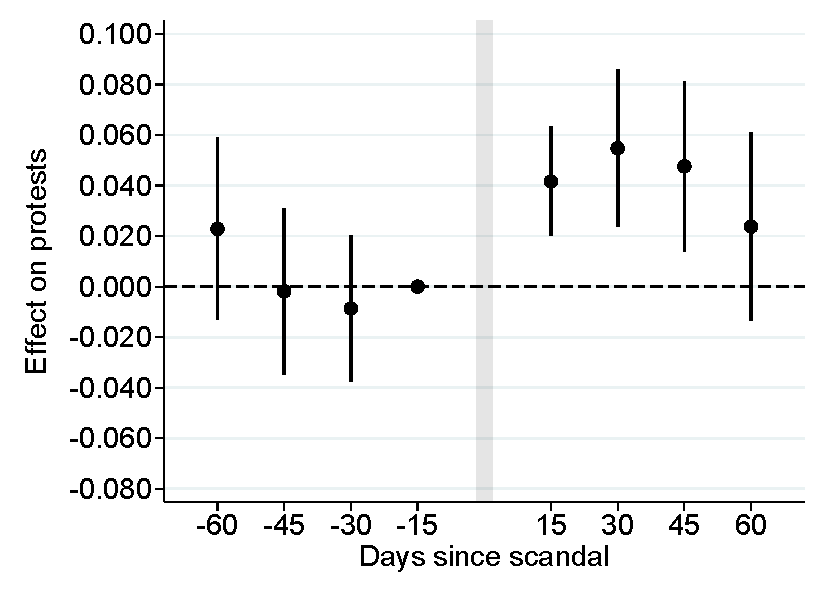
\includegraphics[width=\textwidth]{es_num_violent_MM_w60_b15_pa_ols_90ci.pdf}\label{fig:dynamics:pav}\end{subfigure}\hfill
    \begin{subfigure}{0.45\textwidth}\caption{Peaceful, Apex.}
        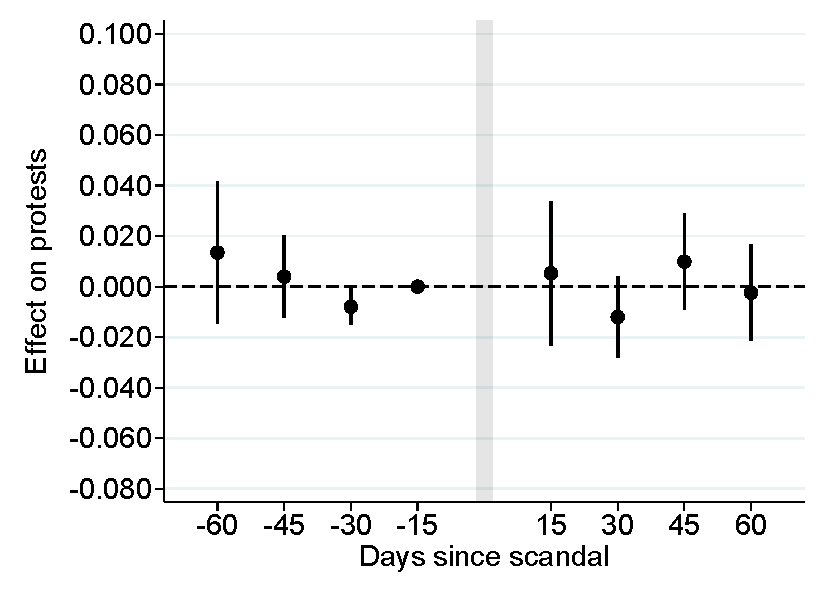
\includegraphics[width=\textwidth]{es_num_peaceful_MM_w60_b15_pa_ols_90ci.pdf}\label{fig:dynamics:pap}\end{subfigure} \\
    \begin{subfigure}{0.45\textwidth}\caption{Violent, Non-Apex.}
        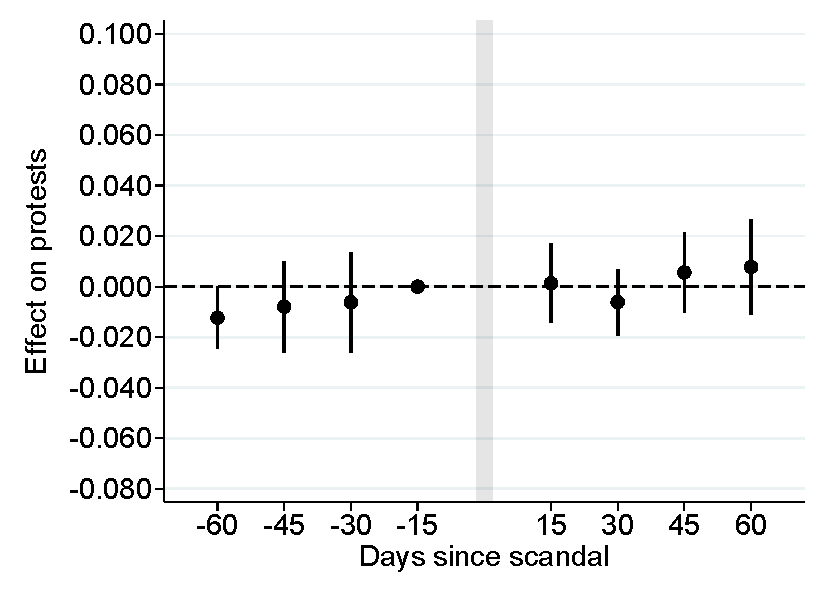
\includegraphics[width=\textwidth]{es_num_violent_MM_w60_b15_na_ols_90ci.pdf}\label{fig:dynamics:nav}\end{subfigure}\hfill
    \begin{subfigure}{0.45\textwidth}\caption{Peaceful, Non-Apex.}
        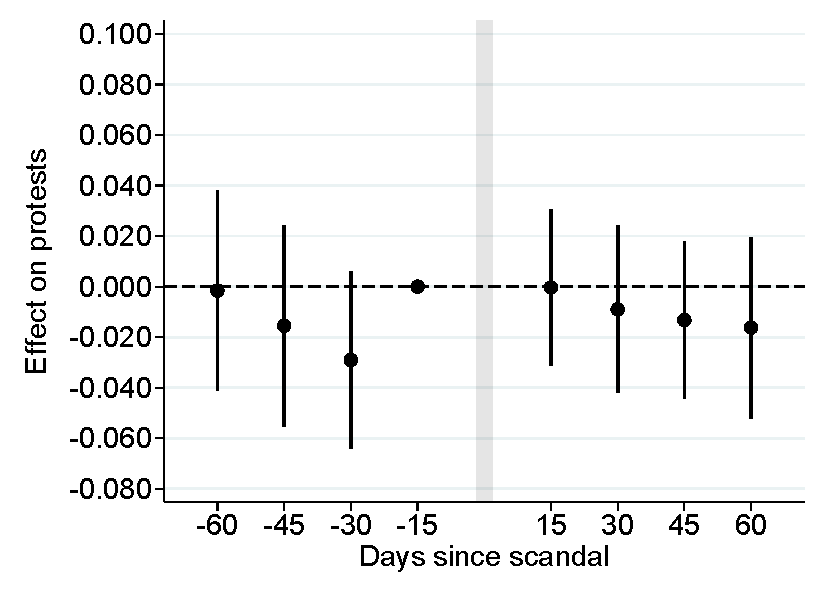
\includegraphics[width=\textwidth]{es_num_peaceful_MM_w60_b15_na_ols_90ci.pdf}\label{fig:dynamics:nap}\end{subfigure}
    \end{center}
    \footnotesize{This figure shows estimates of 15-day time-to-event bin indicators over the $\pm 60$-day window in the modified version of \autoref{eq:main}, estimated separately on the Apex and Non-Apex subsamples. The bin immediately preceding disclosure ($w_{s,t}\in[-15,-1]$) is the reference bin and the faint vertical band marks the disclosure cutoff. Vertical bars are 90\% confidence intervals; standard errors clustered at country $\times$ year $\times$ day-bin. Sample period 2008--2019; Venezuela excluded.}
\end{figure}

\subsection{The protest response is specific to apex corruption}

A natural question is whether the violent-protest response is a general reaction to salient national news, or rather it is specific to apex corruption. To answer this question, in \autoref{tab:uniquetocorruption} we benchmark the corruption effect against two other high-salience national shocks whose timing is plausibly as-good-as-random with respect to the protest baseline: national-team football (soccer) match losses \citep[as in][]{DuranteFutbol} and currency depreciation episodes. We estimate the effect of each ``shock'' by estimating the equation $Y_{c(s)t} \;=\; \beta_{\text{Shock}}\, \mathrm{Post}_{st}\, \;+\; \alpha_d + \lambda_m + \theta_{cy} + \varepsilon_{c(s)t}$, where each variable is defined as in \autoref{eq:main}, except that $\mathrm{Post}_{st}$ is now an indicator for whether date $t$ is after shock $s$. An event in Panel C is a loss of country $c$'s national team, and an event in Panel D is a month-to-month depreciation of the exchange rate of more than 5\%. 

Our findings on Apex and Non-Apex scandals are remarkably similar in this specification as in the one that pooled all scandals together. In the Apex subsample we observe a significant increase in the daily count of violent protests of 0.055 (P$<0.01$) in the 30-day window and of 0.040 (P$<0.01$) in the 60-day window. In the 90-day window we observe a statistically insignificant increase of 0.019 (P$=0.144$) violent protest occurrences. In the 30-, 60-, and 90-day windows we estimate small insignificant changes in peaceful protest occurrences. In the Non-Apex subsample we once again estimate small and insignificant changes in either violent or peaceful protests, with the exception of the 90-day window, in which we estimate an increase in daily protest occurrences of 0.013 (P$<0.1$). Turning to our benchmarks, we also estimate small and insiginificant changes in protest occurrences following football match losses of the national team. For example, in the 30-day window we estimate an insignificant increase in violent protests of 0.006, almost an order of magnitude smaller than the corresponding estimate for Apex scandal disclosures. Similarly, currency depreciations do not seem to generate protests. In fact, in the 60- and 90-day windows we estimate significant 0.012 \textit{decreases} in peaceful protest occurrences (P$<0.1$ in both cases). This evidence is suggestive of the fact that the mobilization response is specific to apex corruption, and not just a general effect in response to salient national events.

\begin{table}[htb!]
    \caption{The effect on violent mobilization is unique to Apex corruption, not generalized across national salient news}
    \label{tab:uniquetocorruption}
    \begin{center}
        \scriptsize{{
\def\sym#1{\ifmmode^{#1}\else\(^{#1}\)\fi}
\begin{tabular}{l*{6}{c}}
\toprule
&\multicolumn{2}{c}{$\pm 30$-Day Window}    &\multicolumn{2}{c}{$\pm 60$-Day Window}    &\multicolumn{2}{c}{$\pm 90$-Day Window}    \\\cmidrule(lr){2-3}\cmidrule(lr){4-5}\cmidrule(lr){6-7}
&\multicolumn{1}{c}{(1)}&\multicolumn{1}{c}{(2)}&\multicolumn{1}{c}{(3)}&\multicolumn{1}{c}{(4)}&\multicolumn{1}{c}{(5)}&\multicolumn{1}{c}{(6)}\\
&\multicolumn{1}{c}{\shortstack{Violent\\Protests}}&\multicolumn{1}{c}{\shortstack{Peaceful\\Protests}}&\multicolumn{1}{c}{\shortstack{Violent\\Protests}}&\multicolumn{1}{c}{\shortstack{Peaceful\\Protests}}&\multicolumn{1}{c}{\shortstack{Violent\\Protests}}&\multicolumn{1}{c}{\shortstack{Peaceful\\Protests}}\\
\midrule \multicolumn{7}{l}{\textbf{\textit{Panel A: Apex}}} \\
Post Event  &       0.055\sym{***}&       0.005         &       0.040\sym{***}&      -0.001         &       0.019         &       0.005         \\
&     (0.016)         &     (0.009)         &     (0.014)         &     (0.008)         &     (0.013)         &     (0.010)         \\
\midrule
Mean (Pre-Event)&       0.028         &       0.015         &       0.037         &       0.019         &       0.045         &       0.021         \\
Observations&        3843         &        3843         &        7623         &        7623         &       11403         &       11403         \\
Number of Events&          63         &          63         &          63         &          63         &          63         &          63         \\
R-squared   &       0.290         &       0.076         &       0.264         &       0.050         &       0.253         &       0.077         \\
\midrule
\multicolumn{7}{l}{\textbf{\textit{Panel B: Non-Apex}}} \\
Post Event  &      -0.003         &       0.011         &       0.008         &       0.001         &       0.011\sym{*}  &      -0.007         \\
&     (0.004)         &     (0.010)         &     (0.006)         &     (0.013)         &     (0.007)         &     (0.011)         \\
\midrule
Mean (Pre-Event)&       0.017         &       0.075         &       0.012         &       0.077         &       0.013         &       0.077         \\
Observations&        6771         &        6771         &       13431         &       13431         &       20091         &       20091         \\
Number of Events&         111         &         111         &         111         &         111         &         111         &         111         \\
R-squared   &       0.121         &       0.571         &       0.110         &       0.472         &       0.085         &       0.406         \\
\bottomrule
\multicolumn{7}{l}{\textbf{\textit{Panel C: Football match losses}}} \\
Post Event  &       0.006         &       0.002         &       0.010         &       0.005         &       0.005         &       0.011         \\
&     (0.005)         &     (0.012)         &     (0.006)         &     (0.013)         &     (0.006)         &     (0.013)         \\
\midrule
Mean (Pre-Event)&       0.009         &       0.043         &       0.013         &       0.036         &       0.010         &       0.036         \\
Observations&       10004         &       10004         &       19844         &       19844         &       29684         &       29684         \\
Number of Events&         164         &         164         &         164         &         164         &         164         &         164         \\
R-squared   &       0.674         &       0.598         &       0.646         &       0.393         &       0.529         &       0.344         \\
\bottomrule
\multicolumn{7}{l}{\textbf{\textit{Panel D: Currency depreciations}}} \\
Post Event  &       0.004         &      -0.003         &      -0.003         &      -0.012\sym{*}  &      -0.007         &      -0.012\sym{*}  \\
&     (0.010)         &     (0.008)         &     (0.007)         &     (0.007)         &     (0.006)         &     (0.006)         \\
\midrule
Mean (Pre-Event)&       0.025         &       0.027         &       0.024         &       0.030         &       0.027         &       0.030         \\
Observations&        9638         &        9638         &       19118         &       19118         &       28598         &       28598         \\
Number of Events&         158         &         158         &         158         &         158         &         158         &         158         \\
R-squared   &       0.331         &       0.275         &       0.348         &       0.169         &       0.346         &       0.144         \\
\bottomrule
\end{tabular}
}
}
    \end{center}
    \footnotesize{This table shows estimates of $\beta_{\text{Shock}}$ in the following equation: $Y_{c(s)t} \;=\; \beta_{\text{Shock}}\, \mathrm{Post}_{st}\, \;+\; \alpha_d + \lambda_m + \theta_{cy} + \varepsilon_{c(s)t}$. The count of violent protests at the country-day level is the outcome in odd-numbered columns, while the count of peaceful protests at the country-day level is the outcome in even-numbered columns. The first two columns use a $\pm30$-day window for the analysis, the next two columns use a $\pm60$-day window for the analysis, and the last two columns use a $\pm90$-day window for the analysis. Panel A shows estimates on the Apex scandals subsample. Panel B shows estimates on the Non-Apex scandals subsample. Panel C shows estimates on the event-windows associated to national-team football match losses. Panel D shows estimates on the event-windows associated to currency depreciation episodes (a month-on-month depreciation of the exchange rate of more than 5\%). An observation is a country-day inside the event window of the corresponding event. All specifications include country-by-year, month-of-year, and day-of-week fixed effects; standard errors (in parentheses) are clustered at the country $\times$ year $\times$ day-bin level. ``Mean (Pre-Event)'' is the average outcome over the same $\pm$window as the column (the 30 days before the event for the $\pm$30 columns, the 60 days before for the $\pm$60 columns, and so on). Sample period 2008--2019; Venezuela excluded. Significance: $^{*}$ $p<0.1$, $^{**}$ $p<0.05$, $^{***}$ $p<0.01$.}
\end{table}

\subsection{Heterogeneity by the level of democracy}

So far we have shown that Apex corruption sparks violent mobilization by citizens, and that this response is not just a generalized response to salient national news. In this section, we further explore whether the effect is driven by countries with different levels of democracy. \textit{Ex-ante} one could think of at least two related, yet opposite, hypotheses about how a country's democratic level interacts with mobilization patterns. On the one hand, citizens in countries with higher levels of democracy may not mobilize, since strong democratic institutions in their countries can punish corrupt officials and remove them from office once proven guilty. On the other hand, precisely because citizens in highly democratic countries have higher standards for accountability, they may choose to mobilize in order to demand democratic institutions to take action. 

To test these hypotheses, we classify the countries in our sample into High/Medium/Low Democracy by their 2008 level of democracy\footnote{We pick 2008 since this is the year in which our sample of scandals starts. Picking later years for the classification would make our democracy measure endogenous to our object of interest.}, as measured by V-Dem's Electoral Democracy Index~\citep{vdem2024}. In particular we classify countries in the bottom tercile of the index's distribution as Low Democracy, those above the bottom tercile but below the top tercile as Medium Democracy, and those in the top tercile as High Democracy\footnote{See \autoref{tab:sup_democracy_index_ranks} for the classification of the countries in our sample.}.

In \autoref{tab:sup_democracy_lmh} we show estimates of an equation analogous to \autoref{eq:main}, but substituting the Apex and Non-Apex indicators for indicators of the country in which the scandal occurs being Low vs. Medium or High Democracy. Contrary to what we expected, the effects are larger---and remarkably consistent across time windows---in countries with higher levels of democracy. In the 30-day window, corruption scandals cause an increase of 0.018 (P$<0.05$) violent protest in countries with higher democratic levels, whereas they only cause a 0.012 (P$<0.05$) increase in the countries with lower democratic levels, though we cannot reject the one-sided hypothesis for the effect being larger than or equal in countries with lower levels of democracy. A similar story is apparent in the 60-day window, where corruption scandals cause an increase of 0.021 (P$<0.05$) in the daily count of violent protests in more democratic countries, and just a 0.010 (P$<0.1$) increase in less democratic ones. Lastly, we estimate an increase of 0.019 (P$<0.05$) daily violent protests in more democratic countries, and a corresponding insignificant 0.001 increase in countries with lower levels of democracy\footnote{We do not find evidence that these patterns can be explained by violent responses of the government towards protestors.}.

\begin{table}[htb!]
    \caption{Effects on violent mobilization are larger in more democratic countries}
    \label{tab:sup_democracy_lmh}
    \begin{center}
        \scriptsize{{
\def\sym#1{\ifmmode^{#1}\else\(^{#1}\)\fi}
\begin{tabular}{l*{6}{c}}
\toprule
            &\multicolumn{2}{c}{$\pm 30$-Day Window}    &\multicolumn{2}{c}{$\pm 60$-Day Window}    &\multicolumn{2}{c}{$\pm 90$-Day Window}    \\\cmidrule(lr){2-3}\cmidrule(lr){4-5}\cmidrule(lr){6-7}
            &\multicolumn{1}{c}{(1)}&\multicolumn{1}{c}{(2)}&\multicolumn{1}{c}{(3)}&\multicolumn{1}{c}{(4)}&\multicolumn{1}{c}{(5)}&\multicolumn{1}{c}{(6)}\\
            &\multicolumn{1}{c}{\shortstack{Violent\\Protests}}&\multicolumn{1}{c}{\shortstack{Peaceful\\Protests}}&\multicolumn{1}{c}{\shortstack{Violent\\Protests}}&\multicolumn{1}{c}{\shortstack{Peaceful\\Protests}}&\multicolumn{1}{c}{\shortstack{Violent\\Protests}}&\multicolumn{1}{c}{\shortstack{Peaceful\\Protests}}\\
\midrule
Post $\times$ Medium+High Democracy (2008)&       0.018\sym{**} &       0.012         &       0.021\sym{**} &       0.000         &       0.019\sym{**} &      -0.005         \\
            &     (0.007)         &     (0.008)         &     (0.008)         &     (0.008)         &     (0.009)         &     (0.007)         \\
Post $\times$ Low Democracy (2008)&       0.012\sym{**} &       0.005         &       0.010\sym{*}  &       0.003         &       0.001         &       0.001         \\
            &     (0.006)         &     (0.014)         &     (0.006)         &     (0.018)         &     (0.005)         &     (0.015)         \\
\midrule
p-value: Medium+High $=$ Low&       0.547         &       0.586         &       0.295         &       0.898         &       0.074         &       0.719         \\
p-value: Medium+High $>$ Low (one-sided)&       0.273         &       0.293         &       0.147         &       0.551         &       0.037         &       0.641         \\
Mean (Pre-Scandal)&       0.020         &       0.053         &       0.021         &       0.056         &       0.024         &       0.057         \\
Observations&       10736         &       10736         &       21296         &       21296         &       31856         &       31856         \\
Number of Scandals&         176         &         176         &         176         &         176         &         176         &         176         \\
R-squared   &       0.160         &       0.473         &       0.154         &       0.396         &       0.133         &       0.348         \\
\bottomrule
\end{tabular}
}
}
    \end{center}
    \footnotesize{This table shows estimates of the effect of apex corruption scandal disclosures on violent and peaceful protests by level of democracy in the country where the scandal occurs. The count of violent protests at the country-day level is the outcome in odd-numbered columns, while the count of peaceful protests at the country-day level is the outcome in even-numbered columns. The first two columns use a $\pm30$-day window for the analysis, the next two columns use a $\pm60$-day window for the analysis, and the last two columns use a $\pm90$-day window for the analysis. ``$p$-value: Medium+High $=$ Low'' reports the two-sided $p$-value for $H_0:\beta_{\text{Medium+High}}=\beta_{\text{Low}}$; ``$p$-value: Medium+High $>$ Low (one-sided)'' reports the one-sided $p$-value. An observation is a country-day inside the event window of the corresponding event. All specifications include country-by-year, month-of-year, and day-of-week fixed effects; standard errors (in parentheses) are clustered at the country $\times$ year $\times$ day-bin level. Sample period 2008--2019; Venezuela excluded. Significance: $^{*}$ $p<0.1$, $^{**}$ $p<0.05$, $^{***}$ $p<0.01$.}
\end{table}

% =====================================================================
% Discussion
% =====================================================================
\section{Discussion}
The evidence we have presented suggests citizens do not respond uniformly to all types of corruption: they respond sharply, immediately and durably when the implicated official is at the apex of the political spectrum, and they barely respond when the implicated official sits at the lower tier of the hierarchy. Furthermore, the response concentrates on violent protests and persists even in a 60-day window. The peaceful margin stays essentially flat over both horizons and regardless of whether the scandal implicates an Apex or Non-Apex politician. Our findings underscore the fact that corruption is a tangible behavioral shock to the local (and perhaps even regional) political environment, not just an attitudinal one. The stakes citizens hold in the continuation in office of a corrupt official appear to govern whether citizens mobilize, and how they do so. The joint pattern of a persistent rise in violent protests with no corresponding change on the peaceful margin is consistent with, though our design does not establish, citizens turning to violent rather than peaceful channels when a scandal undercuts their confidence in the officials meant to be held accountable.

Our findings contribute to three literatures. First, the economics-of-conflict literature has documented that political violence responds to economic shocks~\citep{koenig2017networks,mcguirk2020economic,dube2013commodity,besley2011logic,berman2011hearts,rohner2026aidingpeace}. We introduce a \textit{political} shock---public disclosure of apex corruption---and show that it produces mobilization responses of comparable magnitude to the ones caused by economic shocks. Second, the corruption and accountability literature has documented that disclosures of malfeasance change voting behavior~\citep{ferraz2008exposing,ferraz2011electoral,FerrazFinanAccount,ferraz2018audits,horacio2019infonetwork}. The slow electoral horizon has tended to obscure that the same disclosures can have very fast, non-electoral consequences~\citep{madestam2013protests,bursztyn2021persistent}. Our high-frequency design uncovers a channel through which apex corruption shapes the political environment in democracies within days of public disclosures, well before subsequent elections come into play. Third, the protest channel is the behavioral complement of the attitudinal evidence from our companion paper~\citep{ApexCorruption}, which documents that apex corruption scandals erode support for democracy and democratic institutions, and also reduce political participation.

Our results help reconcile part of the mixed results in the existing literature on the political consequences of corruption disclosures. Studies of local level corruption have produced muted estimates of disclosure's electoral consequences, with some finding modest accountability gains in Brazil and Spain~\citep{ferraz2008exposing,ferraz2011electoral,ferraz2018audits,costasperez2012corruption} and others finding null or even demobilizing effects~\citep{chong2015does,anduiza2013turning,pavao2018corruption,horacio2022metaketa}. We argue that the dispersion in municipal estimates reflects the limited political stakes at that level. In particular, when the implicated official is one of many municipal officeholders, citizens have weaker incentives to incur the costs of mobilization. Within our sample, scandals implicating Congressmen, lower judiciary and lower rank officials have \emph{immediate} (30-day) post-scandal effects on violent protests statistically indistinguishable from zero, whereas the effect of scandals implicating a Apex officials is large and immediate.

A ``salience of stakeholders'' view rationalizes this~\citep{acemoglu2006origins,acemoglu2012nations,jha2013trade,jha2019valuing,jha2022markets}. Citizens' political behavior responds to the political weight of \textit{what} is being disclosed. Apex corruption, thus, affects citizens' perceived stakes of the political bargain, particularly when the implicated official is at the apex of the political hierarchy. The contrast between high--stakes apex scandals and low-stakes lower-officials scandals parallels the contrast between high-stakes elections and routine governance in studies of political accountability~\citep{martinezbravo2022elites}. Notably, this response does not require weak institutions to appear: it is present across our sample and, if anything, somewhat stronger in the more democratic countries, where citizens plausibly hold higher expectations of accountability---and enjoy greater latitude to voice them---when those expectations are violated~\citep{acemoglu2019DemoEcoGrowth,acemoglu2024demobreedsupport,DuranteFutbol}.

Our empirical analyses have some limitations worth noting. Our identification strategy relies on the timing of apex corruption disclosures, not on the timing of the corrupt act itself. If the timing of disclosures is correlated with pre-existing political conditions that affect mobilization (violent or peaceful), our estimates could then be biased. Somewhat reassuringly, the pre-scandal estimates in \autoref{fig:dynamics} show no evidence of pre-existing trends in mobilization. A second limitation comes from the fact that the MM dataset is constructed by looking at news sources reporting on mobilization events. Small protests may thus be underreported as they are not big enough to draw media attention, or protests occurring in geographically remote areas may also be left out. This would induce measurement error in our estimates, but if anything omitting them biases our estimates towards zero. Finally, our scandal sample is limited to Latin American democracies in the 2008--2019 period, thus limiting the external validity of our findings insofar as different regions in the world may mobilize differently in response to corruption scandals. One could also expect different results when shortening/expanding the time scope of the analysis if one believes that the cumulative amount of apex corruption episodes affect the extent to which citizens mobilize.

% =====================================================================
% REFERENCES
% =====================================================================
\clearpage
\bibliography{refs}

% =====================================================================
% SUPPLEMENTARY MATERIALS
% =====================================================================
\clearpage
\appendix
\renewcommand{\thesection}{S\arabic{section}}
\renewcommand{\thesubsection}{S\arabic{section}.\arabic{subsection}}
\renewcommand{\thetable}{S\arabic{table}}
\renewcommand{\thefigure}{S\arabic{figure}}
\setcounter{section}{0}
\setcounter{table}{0}
\setcounter{figure}{0}

\begin{center}
    {\Large\bfseries Supplementary Materials for \\ ``\papertitle''}
\end{center}
\bigskip

\section{Scandal classification}\label{sup:classification}

We classify each of the 176 scandals in our panel by the position of the implicated politician. Using the raw text of the news article reporting on the scandal, we assign a code to the scandal: \texttt{president} for current or former presidents, \texttt{governor} for current or former governors, \texttt{supreme court justice} for Supreme Court Justices, \texttt{congressman} for national legislators, \texttt{other judiciary} for lower-court judges and prosecutors, and \texttt{others} for ministers, agency heads, mayors, and all remaining officials not included in one of the former categories. We then classify scandals in the \texttt{president}, \texttt{governor}, or \texttt{supreme court justice} to the Apex class, and the remaining ones to the Non-Apex class. \autoref{tab:sup_scandal_list} shows the country, year, description and class associated to each of our 176 scandals. 

\begin{landscape}
\begingroup
\setstretch{1.0}\footnotesize
\setlength{\LTcapwidth}{\linewidth}
\begin{longtable}{@{}l c p{15.5cm} l@{}}
\caption{Classification of the 176 scandals in the event-window panel. Rows are in order of occurrence (by disclosure date); this is the same position the leave-one-out figures use to label each scandal. A scandal is \textit{Apex} when the implicated official is a president, governor, or Supreme Court justice, and \textit{Non-Apex} otherwise.}\label{tab:sup_scandal_list}\\
\toprule
\textbf{Country} & \textbf{Year} & \textbf{Description} & \textbf{Class} \\
\midrule
\endfirsthead
\multicolumn{4}{@{}l}{\emph{\tablename~\thetable\ (continued)}}\\
\toprule
\textbf{Country} & \textbf{Year} & \textbf{Description} & \textbf{Class} \\
\midrule
\endhead
\midrule
\multicolumn{4}{r@{}}{\emph{Continued on next page}}\\
\endfoot
\bottomrule
\endlastfoot
Peru & 2008 & On October 5, 2008, this scandal known as Petro-Audios began on Peru, involving Alberto Quimper, manager of Petroperu, and Romulo Leon, ex Minister from APRA (governing party at the time). The scandal ended with the resignation of the Prime Minister of Peru. & Non-Apex \\
Paraguay & 2009 & Fiscala de Coronel Oviedo es imputada por pedido de coima: Una agente del ministerio público y su pareja están & Non-Apex \\
Colombia & 2009 & Agro Ingreso Seguro scandal began on October 8, 2009, when the magazine Cambio de Colombia, denounced that the program had given millionaire subsidies to drug traffickers. The program was designed and implemented by the then Ministry of Agriculture, under the command of Andrés Felipe Arias, under... & Non-Apex \\
Argentina & 2010 & Ricardo Jaime is one of the faces of corruption in Argentina. He has been involved in many corruption accusations. Some of them are on 2009. Besides the media finding out that he had a \$4 million jet (May 22, 2009), he was accused by prosecutor Manuel Garrido of receiving bribes and profiting from... & Non-Apex \\
El Salvador & 2010 & In the night of Saturday, 29 October 2016, the former Salvadorian president Elías Antonio Saca, was captured on alleged corruption charges by the police; according to the Prosecutor, Saca has been arrested for alleged illicit enrichment, unlawful association, and money laundering. Before that,... & Apex \\
Mexico & 2011 & At a press conference on June 24, 2011, Senator Federico Döring exhibited the video that takes up the information and documents delivered to the PGR in the lawsuit against the administrative coordinator of the PRI leadership, Vicente Chaires, and the owner of the SAT of Coahuila, Lorenzo... & Apex \\
Costa Rica & 2011 & On November 29, 2011, the Prosecutor's Office charged deputy Jorge Angulo before Chamber III of the Supreme Court for the alleged commission of seven crimes: four for concussion, two for influence peddling and one for extortion. On June 13, 2012, the Office of the Attorney General of the Republic... & Non-Apex \\
Colombia & 2011 & A los capturados por escándalo en la Dian les imputarán cinco delitos & Non-Apex \\
Paraguay & 2011 & Fiscal de Ciudad del Este es detenido por cobro de supuesta coima. En breve ampliamos. & Non-Apex \\
Peru & 2011 & On October 20, 2011, the benches of Fuerza 2011, Alianza por el Gran Cambio (APGC) and Concertación Parlamentaria presented a constitutional accusation against second vicepresident Chehade for illegal sponsorship, active bribery and influence peddling, for having met with senior police officers to... & Apex \\
Mexico & 2012 & On January 30, 2012, the federal government ended up admitting that since 2009 it began to investigate former Tamaulipas leaders Manuel Cavazos Lerma, Tomás Yarrington Ruvalcaba and Eugenio Hernández Flores, for their alleged links with organized crime. The Attorney General's Office (PGR) has been... & Apex \\
Panama & 2012 & Ricardo Martinelli es vinculado con un acusado de sobornar a Berlusconi . CNN México. 17 de abril de 2012. & Apex \\
Ecuador & 2012 & The Cofiec Duzan scandal begins in 2011, when \$ 800,000 disappeared from an Ecuadorian bank run by the State. The first news regarding this scandal case was on August 20, 2012. & Non-Apex \\
Brazil & 2012 & The Brazilian President, Dilma Rousseff, ordered on November 24, 2012, the dismissal of 18 officials involved in a new corruption scandal, including the head of the Cabinet of the Presidency in Sao Paulo, Rosemary Novoa, as well as directors of the National Water Agency and the National Civil... & Non-Apex \\
Bolivia & 2012 & The Bolivian government faced one of the most serious corruption scandals since the arrival of Evo Morales to power. On November 27, 2012, it was revealed the existence of a network of extortion of inmates that involves senior officials and three prosecutors. & Non-Apex \\
Argentina & 2013 & On April 14, 2013, after two years of investigation, the program Periodismo Para Todos (PPT) denounced an alleged money laundering network that not only splashes but touches former president Néstor Kirchner (who died in October 2010) and his wife, the current president, Cristina Fernández.... & Apex \\
Brazil & 2013 & Lobista envolve líder do governo Dilma em esquema de corrupção. & Non-Apex \\
Chile & 2013 & Revelan que diputada que apoyó Ley de Pesca obtuvo millonaria suma de grupo Angelini previa votación & Non-Apex \\
Peru & 2013 & On January 31 2013, the Prosecutor's Office opened a preliminary investigation to Eva Fernenbug, Toledo's mother-in-law to determine the origin of US \$ 5 million with which she bought a house and a luxury office. The scandal broke as such on May 20 2013, when journalistic programs revealed that two... & Apex \\
Paraguay & 2013 & Detienen por presunta coima a directora administrativa de la Seam & Non-Apex \\
Bolivia & 2013 & Detienen a ocho funcionarios de YPFB por supuesta corrupción: & Non-Apex \\
Brazil & 2013 & Roberto Gurgel: sociedade está cansada da impunidade Ayres Britto também defende manifestações nas ruas & Non-Apex \\
Argentina & 2013 & The military chief Cesar Milani, who faces complaints for his actions in La Rioja and Tucumán between 1976 and 1977, in addition to other questions for alleged illicit enrichment, appeared in the courts to deny the accusations and put himself at the disposal of Justice. On July 30 2013, Federal... & Non-Apex \\
Paraguay & 2013 & Destapan caso niñera de oro, escándalo para el presidente de la cámara Víctor Bogado & Non-Apex \\
El Salvador & 2014 & Francisco Flores was accused in May 2 2014 of pocketing US\$15 million donated by Taiwan, intended for survivors of the January and February 2001 El Salvador earthquakes, which occurred during his presidency. The Prosecutor's Office ordered his arrest. He was investigated since January 9 2014. & Apex \\
Honduras & 2014 & La Comisión Interventora entregó un primer informe en marzo del mismo año, revelando el mayor caso de corrupción y latrocinio en la historia de esa institución, el cual la dejó con una deuda financiera de 6,399.24 millones de lempiras & Non-Apex \\
Brazil & 2014 & The corruption scandal within Petrobras, Brazil's largest company, largely spread on November 14, 2014 with dozens of executives from the country's main construction companies, accused of paying bribes to secure business with the state firm. On March 20, 2014, the scandal begins when former... & Non-Apex \\
Peru & 2014 & Cesar Alvarez, regional president (governor) of Ancash from 2007 to 2014, was arrested in May 2014 as the alleged head of the La Centralita criminal network, which rigged public-works contracts for bribes and ordered killings of political opponents. He was later sentenced to 19.5 years for criminal... & Apex \\
Mexico & 2014 & Lsu interinato en la gubernatura regresó como titular a la Secretaria de Gobierno y permaneció en ella hasta el 4 de abril de 2014 cuando detenido y arraigado por la Procuraduría General de la República acusado de proteger al cártel de los Caballeros Templarios. & Non-Apex \\
El Salvador & 2014 & RT : Bolaños, exministro Gobernación y colaborador, condenados a 3 años por dos delitos: actos arbitrarios y cohecho. & Non-Apex \\
Chile & 2014 & The Penta case, sometimes also called Pentagate, is a Chilean criminal scandal and case, referring to a coordinated and effective fraud against the Chilean Treasury by Empresas Penta, through the use of ideologically false invoices and fees Emitted materially in accordance with the law, but whose... & Non-Apex \\
Panama & 2014 & El panameño Alejandro Moncada Luna, designado magistrado de la Corte Suprema de Justicia de Panamá en enero de 2010 por el entonces presidente Ricardo Martinelli con un salario de 10.000 dólares mensuales, se ha declarado culpable de enriquecimiento injustificado y de falsedad ideológica, y ha sido... & Apex \\
Mexico & 2014 & President Enrique Pena Nieto was implicated in the Casa Blanca conflict-of-interest scandal, revealed on 9 November 2014 by journalist Carmen Aristegui: the president's family occupied an 86-million-peso (about 7-million-dollar) Mexico City mansion built and financed by Grupo Higa, a state... & Apex \\
Chile & 2015 & Los correos políticos que la fiscalía incautó al grupo Penta & Non-Apex \\
Costa Rica & 2015 & Procuradora: Yo no vi el ofrecimiento como soborno \#casosoley & Non-Apex \\
Brazil & 2015 & Em 14 de janeiro de 2015, Nestor Cerveró foi preso pela Polícia Federal, em decorrência das investigações da Operação Lava Jato, acusado de envolvimento nos crimes investigados na Operação Lava Jato. & Non-Apex \\
Argentina & 2015 & Marcelo Tinelli, sobre la muerte de Alberto Nisman: Sensación de impunidad, de impotencia y códigos mafiosos & Non-Apex \\
Chile & 2015 & Fiscalía solicitó formalización de Hugo Bravo por delito tributario, soborno y lavado de activos. & Non-Apex \\
Panama & 2015 & Also, in Panama, on January 28, 2015, an investigation was launched against former president Ricardo Martinelli, with the unanimous vote of all the magistrates of the Supreme Court of Justice, for alleged crimes against the public administration. Ernesto Perez Balladares, another former president... & Apex \\
Panama & 2015 & Declaraciones Tamburelli y Guardia involucran a allegados a Martinelli. Esquema del modus operandi de corrupción PAN. y & Non-Apex \\
Chile & 2015 & On February 5 2015, Qué Pasa magazine published a report in which it stated that the company Exportadora y de Gestión Caval Limitada, owned by Natalia Compagnon - the spouse of Sebastián Dávalos, son of President Michelle Bachelet - had received a loan from the Banco de Chile for more than US \$ 10... & Non-Apex \\
Colombia & 2015 & . reveló video que sería prueba del FBI para demostrar presunto soborno de altos ejecutivos de PetroTiger a exfuncionario de Ecopetrol. & Non-Apex \\
Bolivia & 2015 & Caso Fondo Indigena 12 de febrero de este año tras la publicación de un informe de la Contraloría General del Estado en el que se señalaba 153 fantasmas o fraudulentos & Non-Apex \\
Honduras & 2015 & Firma investigará corrupción en Instituto de la Propiedad. Lea la nota completa en & Non-Apex \\
Mexico & 2015 & The United States joined the investigation carried out by the Mexican Prosecutor's Office against the PAN Governor of Sonora, Guillermo Padrés, for allegedly laundering money from possible bribes from a contractor. & Apex \\
Brazil & 2015 & On April 15, 2016, Brazilian police arrest the treasurer of the ruling Workers Party, João Vaccari, moving the investigation closer to Rousseff s inner circle. Vaccari resigns to focus on his defense. & Non-Apex \\
Guatemala & 2015 & Otto Perez Molina, president of Guatemala, resigned on September 2, 2015 due to his involvement in La Linea corruption scandal, which began on on April 16, 2015, when the International Commission against Impunity in Guatemala and State prosecutors accused a number of politicians in the... & Apex \\
Mexico & 2015 & Audios revelan presuntos sobornos de OHL al gobierno del Estado de México por viaducto Bicentenario & Non-Apex \\
Honduras & 2015 & The first scandal that shook Honduran president Juan Orlando Hernandez' government was the revelation of the use of money from the looting of the Honduran Social Security Institute in Hernández's first presidential campaign, donated through shell companies. Hernández admitted this fact and alleged... & Apex \\
Guatemala & 2015 & \#CasoIGSS | MP y Cicig señalan a Molina Stalling por delitos de asociación ilícita, tráfico de influencias y cobro ilegal de comisiones. & Apex \\
Honduras & 2015 & Fabio Lobo, son of former Honduran president Porfirio Lobo, was arrested on 20 May 2015 for involvement in a drug-trafficking and corruption network. & Non-Apex \\
Panama & 2015 & Cristóbal Salerno revela trama de corrupción en Cobranzas del Istmo & Non-Apex \\
Peru & 2015 & On May 31, 2015 another scandal broke when media found that Venezuelan company Kaysamak C.A. deposited US \$ 87 thousand to former Peruvian first lady Nadine Heredia's mother and friend. & Apex \\
Mexico & 2015 & Ordena Corte Federal de EU captura del exgobernador Eugenio Hernández Flores & Apex \\
Guatemala & 2015 & POLÍTICA: Destino incierto. Expresidente del Congreso pierde su candidatura a diputado, tras escándalo de corrupción. & Non-Apex \\
Brazil & 2015 & PF indicia o ex-diretor da Petrobras Jorge Zelada por corrupção & Non-Apex \\
Guatemala & 2015 & Caso Redes: Gustavo Martínez, ex secretario de Otto Pérez, fue detenido por asociación ilícita y tráfico de influencias. & Non-Apex \\
Peru & 2015 & Documents on alleged economic movements of Nadine Heredia and purchases that she would have made abroad, originated in the Financial Intelligence Unit of Peru, were revealed by the digital medium Ojo-Publico.com in February 2015, when the case began to refloat in Peruvian justice. The confidential... & Apex \\
Guatemala & 2015 & Graban al presidente Otto involucrado directamente en el caso la Linea & Apex \\
Argentina & 2015 & The Pensar Foundation was investigated in an Argentine judicial process initiated in 2015 and closed in 2019. The former president of the Pensar Foundation Matteo Goretti, the former Minister of Culture of Argentina Hernán Lombardi and a former member of the Council for Cultural Promotion of the... & Non-Apex \\
Honduras & 2015 & Pressured by the US embassy in Tegucigalpa, the Honduran Armed Forces (FAH) had to suspend two of their captains, who the US assured since October 7 2016 that they are being investigated for alleged ties to drug trafficking. This happens a year after the United States cornered a Honduran political... & Non-Apex \\
Panama & 2015 & acusación contra Ricardo Martinelli por los pinchazos. \#Corrupción & Apex \\
Argentina & 2015 & The former President Cristina Fernandez is accused of fraudulent administration to the detriment of the State, for the alleged irregular purchase of foreign currency that would have caused millions in losses. The investigation began on October 25, 2015, a judge called Fernandez for inquiry on... & Apex \\
Colombia & 2016 & On January 25, 2016, the Reficar corruption scandal broke. Although for three years they had been talking about the multimillion-dollar costs of the Cartagena Refinery (Reficar), the scandal formally broke out last week when a report by the Comptroller General of the Republic was known about the... & Non-Apex \\
Bolivia & 2016 & Gabriela Zapata, former partner of President Evo Morales, was arrested on February 26, 2016 as part of an investigation into influence peddling of a Chinese company, where she is a commercial manager and which won millionaire public contracts in Bolivia, in a case that ruined the re-election... & Non-Apex \\
Colombia & 2016 & Sigue el duro pulso entre el presidente Santos y el expresidente Uribe tras la captura del ganadero Santiago Uribe. & Non-Apex \\
Brazil & 2016 & Brazilian authorities raided Lula's home. After the raid, the police detained Lula for questioning. & Apex \\
Mexico & 2016 & \#PanamaPapers , ex titular de , niega relación en caso de desvío de fondos & Non-Apex \\
Guatemala & 2016 & El 15 de abril de 2016, a casi un año de descubrir el Caso de La Línea y un día después de que Juan Carlos Monzón fuera aceptado como colaborador eficaz en el caso el Ministerio Público y la CICIG desbarataron otra estructura de corrupción que involucra a los exmandatarios Otto Pérez Molina y... & Apex \\
Bolivia & 2016 & \#LoÚltimo Diputada Norma Piérola: Ministro Juan Ramón Quintana comparecerá el jueves 19 en Diputados por denuncias de tráfico de influencias & Non-Apex \\
Peru & 2016 & The United States Drug Control Administration (DEA) is investigating Joaquín Ramírez, secretary general of the Fuerza Popular party, who is nominating Keiko Fujimori for the presidency of Peru, media reported on May 15 2016. & Non-Apex \\
Ecuador & 2016 & The former manager of Petroecuador, Alex Bravo, is prosecuted for alleged illicit enrichment. According to the investigations, the company Oil Services \& Solutions (OSS) had made commission payments to officials of the state-owned Petroecuador. Bravo was arrested on May 16, 2016. & Non-Apex \\
Ecuador & 2016 & A former manager of Petroecuador (Alex Bravo) was detained on 16 May 2016 for alleged influence peddling. & Non-Apex \\
Brazil & 2016 & El 23 de mayo de 2016, surgió una grabación secreta del ministro Jucá, que está bajo investigación en el esquema de soborno multimillonario en la compañía petrolera estatal Petrobras, discutiendo un supuesto pacto para detener una enorme investigación de corrupción que ha envuelto a gran parte de... & Non-Apex \\
Paraguay & 2016 & Hijo de Sindulfo Blanco niega haber recibido un vehículo como soborno. & Apex \\
Guatemala & 2016 & MP pide procesar a exdiputados por \#PlazasFantasma & Non-Apex \\
Brazil & 2016 & Ministro da Transparência pede demissão após gravações & Non-Apex \\
Guatemala & 2016 & Besides La Linea corruption scandal, Perez Molina was also involved with the la cooperacha scandal, which broke on June 11, 2016. As part of a perverse logic of the exercise of political power, President Otto Perez Molina and Vice President Roxana Baldetti, together with the group of ministers... & Apex \\
Mexico & 2016 & The second scandal, which includes the former, is the Operation Tornado. Since May 2015, many congressmen (mainly from the opposition parties) demanded that the Prosecutor's Office initiate an investigation against the Medina for acts of corruption and the alleged crime of money laundering. In... & Apex \\
Argentina & 2016 & José López was arrested red-handed when he threw the bags over the wall of the convent in the town of General Rodríguez, 50 km west of the Argentine capital, after a neighbor who noticed strange movements called the police, the minister of Security of the province of Buenos Aires, Cristian Ritondo.... & Non-Apex \\
Colombia & 2016 & On May 10 2017, it was known that the former governor of Córdoba, Alejandro Lyons, fled to avoid being convicted of embezzlement, for amounts that amounted to 10,000 million pesos at that time (USD \$ 3,322,260), according to the record, in events that occurred during his administration. On January... & Apex \\
Mexico & 2016 & En 2016 la revista Expansión junto con Mexicanos contra la corrupción y la impunidad publicó la investigación Los Piratas de Borge, donde denuncian una maquinaria institucional compuesta por funcionarios públicos y notarios auspiciados por el gobernador Roberto Borge que arrebataba el patrimonio a... & Apex \\
El Salvador & 2016 & La Fiscalía capturó este lunes 22 de agosto a quien hasta hace solo ocho meses era fiscal general: Luis Martínez. Horas antes había capturado a Enrique Rais, & Non-Apex \\
Guatemala & 2016 & Familia de Jimmy Morales declara por caso de corrupción. Escuche lo que dijo el mandatario & Apex \\
Brazil & 2016 & On September 26, 2016, former minister Antonio Palocci was arrested by the Federal Police of Brazil, at the request of the latter and authorized by federal judge Sergio Moro, in the 35th phase of the Lava Jato, named Omertà. He was investigated since June 15 2015. & Non-Apex \\
Ecuador & 2016 & Carlos Pareja, a former official who has held strategic positions in the hydrocarbons sector since the current Ecuadorian government started in 2007, left the country before he was linked to the Petroecuador corruption case. He was arrested in Peru on May 8, 2017. & Non-Apex \\
Mexico & 2016 & On September 14, 2014, lawyer Jaime García Chávez criminally denounced Governor Duarte before the Attorney General's Office for the crimes of embezzlement, illicit enrichment, abusive exercise of functions and improper use of powers and powers. On March 28, 2017, an arrest warrant had been issued... & Apex \\
Dominican Republic & 2016 & Casos Tucanos & Non-Apex \\
Ecuador & 2016 & Inician detenciones por Caso Odebretch en Ecuador con el exe ministro de energia Mosqueda & Non-Apex \\
El Salvador & 2016 & : A. Saca, Élmer Charláix, Pablo Gómez y Fco. Rodríguez acusados por delitos de Peculado, Agrupaciones Ilícitas y Lavado de Dinero. & Apex \\
Brazil & 2016 & On June 22, 2016, Sergio Cabral, former governor of Rio, was accused of charging 5\% on every contract awarded to Odebrecht, including those for restoring the Maracanã stadium and the Coperj railroad. On November 17, 2016, the Federal Police of Brazil arrested Sérgio Cabral and seven other persons.... & Apex \\
Mexico & 2017 & Four former Mexican governors reportedly received bribes from Luis Carlos Castillo Cervantes El Rey de los Dragones, after inflating the cost of paving works, according to a statement from the Attorney General's Office for the Southern District of Texas. Those involved are Humberto Moreira,... & Apex \\
Colombia & 2017 & On January 13, 2017 it was revealed that Gabriel García Morales, former Deputy Minister of Transportation in Álvaro Uribe's government, is the first Colombian involved in the corruption of the Brazilian construction firm. According to the attorney general, García was paid US \$ 6.5 million so that... & Non-Apex \\
Guatemala & 2017 & On January 18, 2017, the brother and a son of the country s president, who swept to victory with an anti-graft campaign, were arrested for their alleged involvement in corruption. & Non-Apex \\
Peru & 2017 & On January 20, 2017, Edwin Luyo was arrested in Peru for his involvement in the Odebrecht corruption scandal. Former official Edwin Luyo was accused by the Public Ministry of having received money from the Brazilian company to favor it in the tender for the construction of line 1 of the metro in... & Non-Apex \\
Chile & 2017 & 23 de enero de 2017, una investigación publicada en Ciper hizo pública una conversación vía correo electrónico entablada en 2014 entre Jacqueline Van Rysselberghe y Luis Felipe Moncada, presidente de la Asociación de Industriales Pesqueros del BíoBío (Asipes), mientras la primera dirigía la... & Non-Apex \\
Panama & 2017 & Panamanian justice began on January 24 2017 the search for the first 17 people required in the case of the Odebrecht bribes, among them two sons of former President Ricardo Martinelli, to whom Switzerland froze accounts with 22 million dollars. & Apex \\
Peru & 2017 & The former president of Peru, Alejandro Toledo (2001-2006) received a millionaire bribe from the Brazilian Odebrecht in exchange for a public work, according to information handled by the prosecution, the Peruvian press reported on February 3, 2017. & Apex \\
Colombia & 2017 & On Febrary 8, 2017, Colombian authorities investigate whether Juan Manuel Santos' presidential campaign received US \$ 1 million from Odebrecht. Around the same dates, Óscar Iván Zuluaga, presidential candidate of the party led by the former Colombian president in the elections in which Santos won... & Apex \\
Panama & 2017 & Panama's President Juan Carlos Varela has been accused by a former advisor Ramon Fonseca of taking donations from Odebrecht. & Apex \\
Mexico & 2017 & El 20 de febrero de 2017 la policía de Veracruz halló una bodega en Córdoba, Veracruz con objetos pertenecientes a Javier Duarte y Karime Macías.125 En ella fueron hallados objetos de asistencia social como sillas de ruedas y despensas; objetos suntuosos como obras de arte, palos de golf, vajillas,... & Apex \\
Mexico & 2017 & On February 21, 2017, it was revealed that the Ministry of Social Development (Sedesol) diverted at least 1,787 million pesos in 2015, the year in which the agency was successively headed by Rosario Robles Berlanga, now head of the Ministry of Agrarian, Territorial and Urban Development (Sedatu),... & Non-Apex \\
Honduras & 2017 & Devis Leonel Rivera Maradiaga, exlíder del cartel de Los Cachiros, quien se entregó a la DEA en diciembre de 2015, testificó el día lunes 6 de marzo de 2017 ante un tribunal de Nueva York a pedido del gobierno de Estados Unidos de América, en el marco del caso contra el hijo del exmandatario, Fabio... & Non-Apex \\
Mexico & 2017 & El 27 de marzo de 2017, fueron arrestados Javier Garfio Pacheco y Gerardo Villegas Madriles, exsecretario de obras públicas y exadministrador de la Secretaría de Hacienda del Gobierno de Chihuahua, acusados de peculado. Esa misma tarde, en conferencia de prensa, el gobernador de Chihuahua, Javier... & Apex \\
Peru & 2017 & On April 3, 2017, Peruvian Mayor Felix Moreno is investigated for his involvement in the Odebrecht scandal. & Non-Apex \\
Brazil & 2017 & On April 11 2017, Odebrecht recognizes payments of more than US \$ 4 million to Lula da Silva. & Apex \\
Peru & 2017 & Marcelo Odebrecht confirmó la entrega de USD 3 millones al ex presidente peruano Ollanta Humala & Apex \\
Brazil & 2017 & President Michel Temer was implicated on 17 May 2017 when a covert recording released through the JBS (Batista brothers) plea bargain appeared to capture him endorsing hush-money payments to jailed former House speaker Eduardo Cunha. Prosecutors charged him with passive corruption and obstruction;... & Apex \\
Brazil & 2017 & Ex-governadores de Brasília são presos por corrupção na Copa & Apex \\
Dominican Republic & 2017 & En la mañana del 29 de mayo de 2017 el procurador general de la República, Jean Alain Rodríguez, implicó a 14 hombres entre ellos, empresarios, políticos (incluidos un ministro) y un abogado de ser parte del entramado de corrupción de Odebrecht. & Non-Apex \\
Ecuador & 2017 & Ecuador's Prosecutor's Office charged six people on 3 June 2017 in the Odebrecht case, among them Ricardo Rivera, uncle of Vice-President Jorge Glas. & Non-Apex \\
Ecuador & 2017 & El 2 de junio de 2017, se realizaron operaciones coordinadas por la Fiscalía General del Estado en relación con el caso Odebrecht, resultando en la detención de Ricardo Ramírez, tío del vicepresidente Jorge Glas, encargado de varios negocios cuando Glas era ministro durante el gobierno de Rafael... & Non-Apex \\
Colombia & 2017 & Audios prueban que la española Inassa sobornó a políticos colombianos y & Non-Apex \\
Mexico & 2017 & Alleged corruption network involving diputados (congressmen) in San Luis Potosi, Mexico; trended nationally on 21 June 2017 after a Denise Maerker report. & Non-Apex \\
Argentina & 2017 & On June 18, 2017, the direct environment of the former Minister of Federal Planning Julio De Vido agreed to a bribe for US \$ 25 million and other unconventional practices in exchange for unblocking the access of the Brazilian construction company Odebrecht to a multi-million dollar project for the... & Non-Apex \\
Mexico & 2017 & Gobierno mexicano espía a periodistas, activistas y líderes con software Pegasus: The New York Times & Non-Apex \\
Colombia & 2017 & The director of the National Anticorruption Prosecutor's Office of Colombia, Luis Gustavo Moreno, was arrested on June 27, 2017 in his offices, on charges of alleged money laundering. On March 7 2018, he was sentenced. & Non-Apex \\
Colombia & 2017 & Fue capturado el Director Nacional Contra la Corrupción de . & Non-Apex \\
Panama & 2017 & On November 20, the first one condemns the case in this country: Jorge Espino, a businessman who confessed to having been an intermediary for former Public Works minister Jaime Ford to receive US\$ 1.8 million in bribes from Odebrecht. Demetrio Papadimitriu, former minister of the presidency, and... & Non-Apex \\
Costa Rica & 2017 & On June 28 2017, 'Cementazo' scandal broke in Costa Rica, where the loan of \$ 31.5 million from the Bank of Costa Rica (BCR, a state bank) to the construction businessman Juan Carlos Bolaños and his company Sinocem Costa Rica in irregular conditions is questioned. & Non-Apex \\
Ecuador & 2017 & Fiscal General anuncia pruebas de corrupción de Carlos Pólit--> & Non-Apex \\
Peru & 2017 & On July 13, 2017, Peruvian justice dictates 18 months of preventive prison to the Humala for the Odebrecht case. On May 7, 2019, the Peruvian Attorney Office asked for a 20 years sentence to him and 26 years to his wife. & Apex \\
Brazil & 2017 & Lula é condenado a 9 anos por corrupção no tríplex & Apex \\
Colombia & 2017 & The investigators of the Odebrecht case claim to have evidence that through Básima Patricia Elías Náder - cousin sister of Senator Bernardo 'Ñoño' Elías and hostess of presidents and congressmen-, several of the multinational's bribes were channeled to obtain the otheri from the via Ocaña-Gamarra.... & Non-Apex \\
Guatemala & 2017 & Corrupción Micivi: Empresas que pagaron sobornos han recibido 6.7 millardos del Estado & Non-Apex \\
Argentina & 2017 & Filman a un intendente de Santa Cruz y después lo denuncian por recibir una coima de 2 millones de pesos & Non-Apex \\
Bolivia & 2017 & \#LoÚltimo Detienen al Director Nacional de Derechos Reales, Jorge Bohorquez, por actos de corrupción y extorsión, informa & Non-Apex \\
Ecuador & 2017 & On August 3 2017, the president of Ecuador, Lenín Moreno, stripped Vice President Jorge Glas, involved in the Odebrecht case, of his powers. Glas would have been part of a bribery network; he is investigated by the prosecution. On December 13, 2017, Glas was sentenced for the crime of illicit... & Apex \\
Mexico & 2017 & Tres exdirectivos de Odebrecht aseguran que Emilio Lozoya, exdirector de Pemex y colaborador del presidente, recibió 10 millones de dólares en sobornos & Non-Apex \\
Ecuador & 2017 & On August 18, 2017, the Ecuadorian Prosecutor's Office carried out an operation to capture former minister Ramiro González Jaramillo, accused of an alleged tax fraud. A preventive arrest order was issued against him and his properties and the headquarters of the Avanza Party in Quito were raided.... & Non-Apex \\
Colombia & 2017 & On August 29, 2017, the Colombian senator for the U Party, Musa Besaile, admitted that he paid 2,000 million pesos to magistrates of the Supreme Court of Justice (such as Luis Gustavo Moreno) as part of an extortion, which would stop his arrest warrant in the process for parapolitics. The cartel de... & Non-Apex \\
Brazil & 2017 & The Brazilian Federal Police (PF) yesterday found suitcases and boxes full of money in an apartment that, apparently, was used by former minister Geddel Vieira Lima, a former and close collaborator of President Michel Temer arrested for alleged corruption. & Non-Apex \\
Mexico & 2017 & La Estafa Maestra is the name of a journalistic investigation carried out by the Mexican news portal Animal Político in association with the civil society organization Mexicanos Contra la Corrupción y la Impunidad (MCCI). Published on September 5, 2017, the investigation unraveled a system of 128... & Non-Apex \\
Guatemala & 2017 & The former Minister of Defense of Guatemala, retired General Williams Mansilla Fernández, was arrested today on charges of corruption, because he authorized an illegal extraordinary bonus that he paid to President Jimmy Morales and high-ranking Army commanders. & Non-Apex \\
Argentina & 2017 & Julio De Vido en la causa por las irregularidades en Yacimientos Carboníferos Río Turbio. & Non-Apex \\
Costa Rica & 2017 & Fiscalía investiga si Celso Gamboa incurrió en abuso de autoridad y tráfico de influencias & Non-Apex \\
Argentina & 2017 & The Paradise Papers in Argentina refer to the local repercussion of the scandal pro tax evasion and ownership of offshore companies in tax havens, after the worldwide revelation of 13.4 million documents related to investments in tax havens, leaked to the public on November 5, 2017. Argentinian... & Non-Apex \\
Peru & 2017 & The former mayor of Lima Susana Villarán spoke yesterday on the statement that the Brazilian businessman Valdemir Garreta gave to the Peruvian prosecutor's office, in which he affirmed that he had received US \$ 3 million from Odebrecht and OAS as payment for the advertising and consultancies... & Non-Apex \\
Honduras & 2017 & El equipo integrado UFECIC-MACCIH descubrió a través de sus fiscales e investigaciones una Red de Diputados que se apropió ilegalmente de fondos públicos destinados a proyectos sociales que fueron desviados para uso personal. & Non-Apex \\
Peru & 2017 & On December 13 2017, it became public that the Brazilian construction company Odebrecht, prosecuted for corruption, admitted that it paid consultancies for almost 5 million dollars to two companies linked to the current president of Peru, Pedro Pablo Kuczynski, who will now have to give... & Apex \\
Peru & 2018 & The Construction Club is the name given to an alleged illicit concertation of construction companies in Peru (between nationals and foreigners) to distribute works awarded by the Ministry of Transport and Communications of Peru (MTC). The first revelation of the club was on July 7 2017. On May 21,... & Non-Apex \\
Guatemala & 2018 & EEUU detiene a excandidato presidencial de Guatemala vinculado con escándalo Odebrecht & Non-Apex \\
Guatemala & 2018 & Álvaro Colom y varios exministros son capturados por \#CasoTransurbano. Algunos exfuncionarios ya han llegado a Torr & Apex \\
Honduras & 2018 & Former First Lady of Honduras Rosa Elena Bonilla, wife of former Honduran President Porfirio Lobo (2010-2014), was arrested yesterday, accused of abuse of power and illicit enrichment. According to El Heraldo, the justice opened an investigation into Bonilla for the case of transfers to personal... & Apex \\
Peru & 2018 & On February 28 2018, the former head of Odebrecht in Peru Jorge Barata told Peruvian prosecutors during a court hearing in Brazil that he provided money for the electoral campaigns of President Pedro Pablo Kuczynski and former presidential candidate Keiko Fujimori. On June 10 2018, the Peruvian... & Apex \\
Peru & 2018 & The Kenjivideos scandal is a political scandal that began in Peru on March 20 2018 as part of the currently ongoing political crisis. It followed the release of videos filmed by Congressman Moisés Mamani showing opposition congressmen offering construction projects and special access to the... & Apex \\
El Salvador & 2018 & The Attorney General of El Salvador ordered on Friday, June 8, 2018, the capture of Funes, several of his former officials and family members accused of participating in acts of corruption through which they appropriated state funds for 351 million dollars. Presidential House (CAPRES) used the... & Apex \\
Honduras & 2018 & Se exhibe caso pandora. & Non-Apex \\
Colombia & 2018 & Fiscal general de la Nación, Néstor Humberto Martínez, entregó detalles de una red de corrupción al servicio de var & Non-Apex \\
Colombia & 2018 & Senator Antonio Jose Correa was the first legislator named in Colombia's mermelada toxica (toxic pork-barrel) scandal: on 5 July 2018 the Prosecutor's Office referred him for allegedly taking a roughly 12-percent kickback on a 3.49-billion-peso Coldeportes sports-infrastructure contract. In 2023... & Non-Apex \\
Nicaragua & 2018 & El subdirector de la Policía Nacional, consuegro de Daniel Ortega, y el tesorero del FSLN son los dos funcionarios & Non-Apex \\
Nicaragua & 2018 & El subdirector de la Policía Nacional, consuegro de Daniel Ortega, y el tesorero del FSLN son los dos funcionarios & Non-Apex \\
Paraguay & 2018 & Cae funcionario de la Corte con presunta coima . & Non-Apex \\
Peru & 2018 & On Saturday, July 7, 2018, the news portal IDL-Reporters broadcast a series of audios that involve officials of the National Council of the Judiciary and judges who could have committed influence and corruption trafficking. Among the names committed are in addition to Hinostroza the current... & Non-Apex \\
Paraguay & 2018 & \#CaserosDeOro Para evitar el juicio oral y público, el diputado José María Ibáñez reconoció los hechos y ofreció re & Non-Apex \\
Argentina & 2018 & Argentina was shaken on Wednesday August 1 2018 by a new corruption scandal, for the alleged payment of millionaire bribes, which led to a dozen arrests of former officials of the Cristina Fernández government and businessmen, including a former director linked to the group of President Macri's... & Non-Apex \\
Peru & 2018 & On 10 October 2018, Fujimori was arrested and placed in provisional detention on charges of money laundering days after the Supreme Court of Peru nullified the pardon of her father, ordering him back to prison. The arrest order stated that she led a criminal organization inside of Fuerza 2011... & Non-Apex \\
El Salvador & 2018 & Former Salvadorian Attorney General Luis Martinez was accused on October 18, 2018 of accepting bribes to obtain benefits from the prosecutor's office, specifically to lease a property owned by a company in which Mr. Parducci is a shareholder and legal representative. & Non-Apex \\
Honduras & 2018 & Inicia el escandalo conocido con caja chica del hermano & Non-Apex \\
Peru & 2018 & The Peruvian prosecutor José Domingo Pérez, in charge of the investigations in Peru of the Odebrecht case, today asked a judge to prevent former President Alan García from leaving the country for allegedly having received illicit payments from the Brazilian construction company. On November 18... & Apex \\
Honduras & 2018 & \#caso arca abierta requerimiento fiscal contra cinco diputados y seis ex diputados hondureños por el presunto delito de malversación de caudales públicos en perjuicio de la Administración Pública del Estado de Honduras & Non-Apex \\
Peru & 2019 & Four hours before the end of 2018, the Peruvian prosecutor, Pedro Gonzalo Chávarry, had the idea of dismissing two of the prosecutors investigating the Odebrecht case. The dismissal of the two most important prosecutors in the Odebrecht case, who had been in office for six months, comes a week... & Non-Apex \\
El Salvador & 2019 & Attorney General Office opens investigation against former Salvadorian president Mauricio Funes for purchase of deputies. & Apex \\
Guatemala & 2019 & Capturados hasta ahora por caso de \#FinanciamientoUNE son: - Exsecretario privado de la Presidencia (en tiempos de & Non-Apex \\
Peru & 2019 & On 17 April 2019, former Peruvian presiden Alan García died from a self-inflicted gunshot to the head as police officers were preparing to arrest him over matters relating to the Odebrecht scandal. & Apex \\
Peru & 2019 & Miguel Atala, ex vicepresidente de PetroPerú, confesó a la fiscalía que sirvió de testaferro para que el ex preside & Apex \\
Guatemala & 2019 & El \#CasoCompradeVotos que golpea a siete partidos políticos en pleno año electoral & Non-Apex \\
Mexico & 2019 & The United States Department of the Treasury declared Roberto Sandoval Castañeda and judge Isidro Avelar Gutiérrez significant drug dealers on May 17, 2019. Six other individuals and six corporations were similarly sanctioned. & Non-Apex \\
Honduras & 2019 & On May 30, 2019, US prosecutors unsealed some 2015 documents which revealed that Hernández was himself the subject of a major drug trafficking and money laundering investigation, alongside his sister Hilda and others. & Apex \\
Dominican Republic & 2019 & \#PeriódicoHOY Piden la renuncia inmediata del presidente Danilo Medina por soborno de US\$39.5 millones en Punta Cat & Apex \\
Honduras & 2019 & On August 3, 2019, Honduran President Juan Orlando Hernández was identified Friday as a co-conspirator in a drug trafficking and money laundering case against his brother, according to document filed in U.S. district court. Prosecutors say \$1.5 million in drug proceeds was used to help elect him in... & Apex \\
Peru & 2019 & Pedro Chávarry: juez decidió abrir proceso penal a exfiscal de la Nación & Non-Apex \\
Honduras & 2019 & On October 8, 2019, a former Honduran mayor, who appears before a trial for drug trafficking, declared and pointed to the current president of Honduras Juan Orlando Hernández, as the person who received a million dollars (\$ 1 million) to pay for the campaign to the National Congress of Honduras, of... & Apex \\
Mexico & 2019 & President Andrés Manuel López Obrador revealed that the United States government notified the Financial Intelligence Unit (UIF) of the Ministry of Finance and Public Credit (SHCP) about the case of irregular movements of the minister's bank accounts abroad of the Supreme Court of Justice of the... & Apex \\
Panama & 2019 & The judge of the National Court Ismael Moreno has accused the Spanish multinational Fomento de Construcciones y Contratas (FCC) as a legal entity for paying bribes of more than 82 million euros to obtain public works awards in Panama. Also, it is being investigated whether the president of Panama... & Non-Apex \\
Paraguay & 2019 & On November 20, 2019, operation Lava Jato, in which the largest corruption scandal in the history of Brazil is being investigated, has hit Paraguayan politics with a prison order against former President Horacio Cartes, accused of participating in a transnational criminal network dedicated to money... & Apex \\
\end{longtable}
\endgroup
\end{landscape}


% ---------------------------------------------------------------------
\clearpage
\section{The timing of scandal disclosures is unpredictable}\label{sup:random}



Our identification rests on the exact calendar date of a scandal's disclosure being as-good-as-randomly distributed \emph{within} a country-year. We ask whether the day a scandal is disclosed can be told apart from the other days of the \emph{same} country-year using calendar structure and the electoral cycle. We estimate a conditional---on country-by-year fixed-effects---logit and measure discrimination with the within-country-year AUC. That is, the probability the model ranks the true scandal-day above a random non-scandal-day of the same country-year.

\begin{table}[htb!]
    \caption{Predicting the exact disclosure date within a country-year.}
    \label{tab:scandal_random}
    \begin{center}\begin{tabular}{lcccc}
\toprule
 & (1) & (2) & (3) & (4) \\
\midrule
Day of week & Yes & Yes & Yes & Yes \\
Month of year & No & Yes & Yes & Yes \\
Day of month & No & No & Yes & Yes \\
Election proximity & No & No & No & Yes \\
Country $\times$ year FE & Yes & Yes & Yes & Yes \\
\midrule
Country-days &    28,852 &    28,852 &    28,852 &    28,852 \\
Scandal country-years &   79 &   79 &   79 &   79 \\
Joint test $p$-value & 0.010 & 0.003 & 0.123 & 0.164 \\
Within-year AUC (in-sample) & 0.591 & 0.642 & 0.679 & 0.682 \\
Within-year AUC (out-of-sample) & 0.562 & 0.583 & 0.552 & 0.537 \\
\bottomrule
\end{tabular}
\end{center}
    \footnotesize{This table shows how well the exact disclosure date of a corruption scandal can be predicted \emph{within} a country-year, using progressively richer sets of predictors. Each column is a conditional (country-by-year fixed-effects) logit of an indicator for a scandal being disclosed on a given country-day, on the day of the week, the month of the year, the day of the month, and proximity to a national election (indicators for a day falling 0--30, 31--60, 61--90, or 91--120 days before an election), with each column adding one predictor set to the previous. An observation is a country-day; conditioning on country-by-year restricts the comparison to the 79 country-years that contain a scandal (28{,}852 country-days), and our 176 scandals fall on 171 distinct country-days. ``Joint test $p$-value'' is the Wald test that the predictors added in that column jointly matter. ``Within-year AUC'' is Harrell's $c$ restricted to within-country-year comparisons---the probability the model ranks the true scandal-day above a random non-scandal-day of the same country-year, where $0.5$ is a coin flip---and the out-of-sample row trains on a random half of the country-days and evaluates on the held-out half. Sample period 2008--2019; Venezuela excluded.}
\end{table}

% ---------------------------------------------------------------------
\clearpage
\section{Sensitivity to the event-window width}\label{sup:window}

We re-estimate the OLS specification at every event-window width $T \in \{15, 30, 45, \dots, 150\}$ days and plot the point estimate against $T$ with a 90\% confidence interval. \autoref{fig:sup_window} places the Apex and Non-Apex subsamples \emph{side by side}---violent protests in the top row, peaceful in the bottom---on a \emph{common y-axis across all four panels}. The $T=30, 60, 90$ window-widths reported in Table~\ref{tab:uniquetocorruption} are shown with diamond markers.

\begin{figure}[htb!]
    \caption{Window-width sensitivity: Apex vs.\ Non-Apex.}
    \label{fig:sup_window}
    \begin{center}
    \begin{subfigure}{0.48\textwidth}
        \caption{Violent, Apex.}
        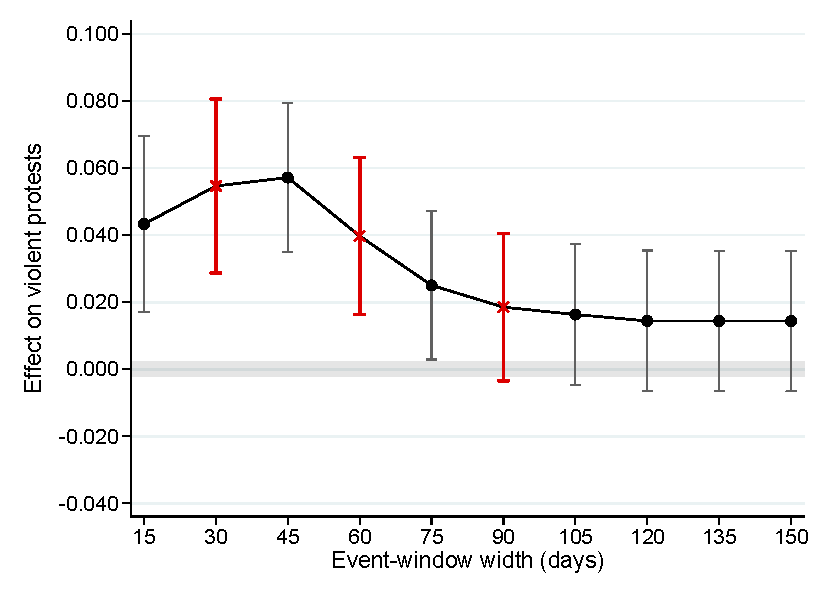
\includegraphics[width=\textwidth]{sup_window_sensitivity_ols_num_violent_MM_pa.pdf}
    \end{subfigure}\hfill
    \begin{subfigure}{0.48\textwidth}
        \caption{Violent, Non-Apex.}
        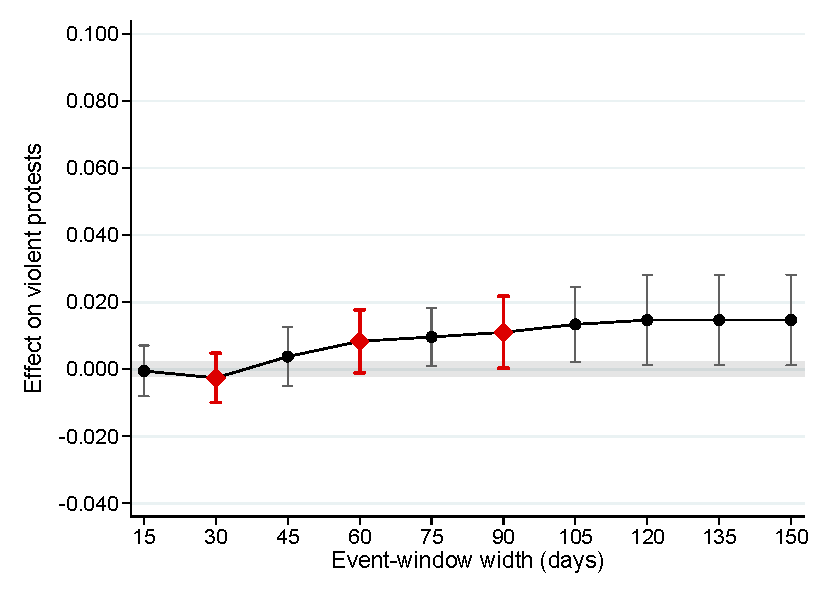
\includegraphics[width=\textwidth]{sup_window_sensitivity_ols_num_violent_MM_na.pdf}
    \end{subfigure} \\
    \begin{subfigure}{0.48\textwidth}
        \caption{Peaceful, Apex.}
        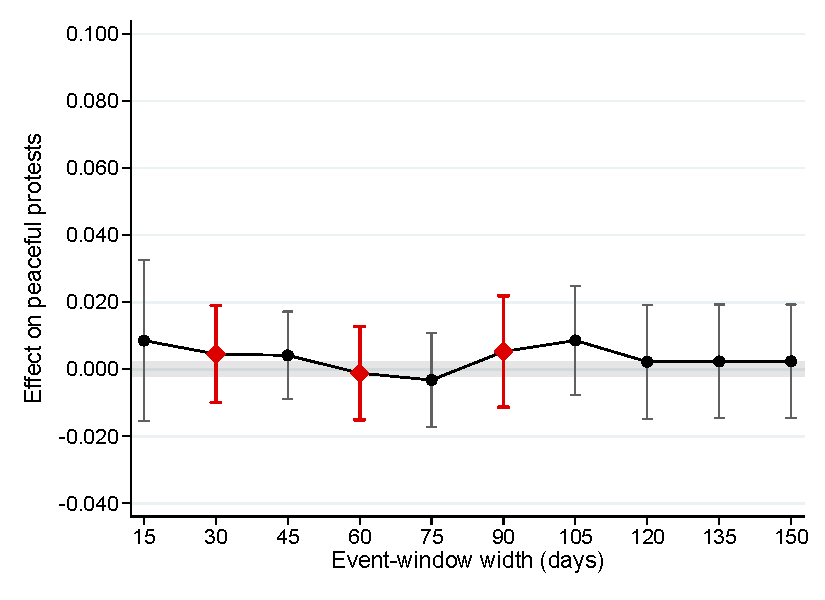
\includegraphics[width=\textwidth]{sup_window_sensitivity_ols_num_peaceful_MM_pa.pdf}
    \end{subfigure}\hfill
    \begin{subfigure}{0.48\textwidth}
        \caption{Peaceful, Non-Apex.}
        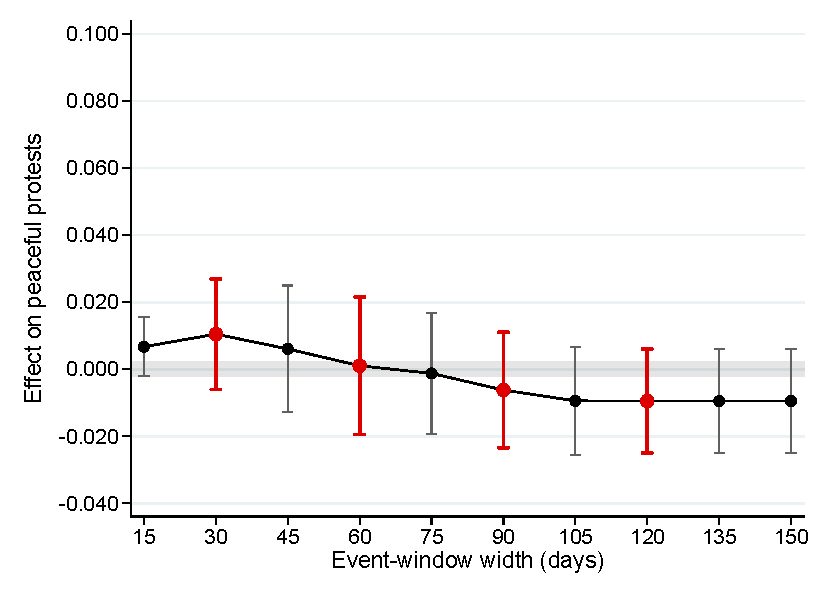
\includegraphics[width=\textwidth]{sup_window_sensitivity_ols_num_peaceful_MM_na.pdf}
    \end{subfigure}
    \end{center}
    \footnotesize{For each $T \in \{15, 30, \dots, 150\}$ we re-estimate the OLS specification on the event-window panel restricted to $|w_{st}|\leq T$, separately on the 63 Apex and 113 Non-Apex scandals. Vertical bars are 90\% confidence intervals; the markers at $T=30, 60, 90$ (the widths in Table~\ref{tab:uniquetocorruption}) are highlighted in red. All four panels share a common y-axis. Sample period 2008--2019; Venezuela excluded.}
\end{figure}

% ---------------------------------------------------------------------
\clearpage

% ---------------------------------------------------------------------
\section{Randomization inference by apex-partition subsample}\label{sup:ri}

We complement the headline estimates with a randomization-inference (permutation) test, run separately on the two subsamples used for Panel A and Panel B of Table~\ref{tab:uniquetocorruption}. In each of 1{,}000 replications and for each scandal we draw a placebo disclosure date uniformly at random within the scandal's original country-year, rejecting any draw whose $\pm T$-day window would overlap a real disclosure date in the same country (with an unconditional fallback over all countries and 2008--2019 dates after 20 failed within-country-year attempts). We rebuild the $\pm T$-day event-window panel around the placebo dates and re-estimate the OLS specification. Figures~\ref{fig:sup_ri_violent} and \ref{fig:sup_ri_peaceful} plot the resulting placebo $\hat\beta$ distributions; the maroon vertical line marks the observed $\hat\beta$ from the corresponding cell of Table~\ref{tab:uniquetocorruption}, and the legend reports that observed $\hat\beta$ together with the two-sided randomization-inference $p$-value. 

\begin{figure}[htb!]
    \caption{Randomization inference: violent protests.}
    \label{fig:sup_ri_violent}
    \begin{center}
    \begin{subfigure}{0.32\textwidth}\caption{Apex, $\pm 30$.}
        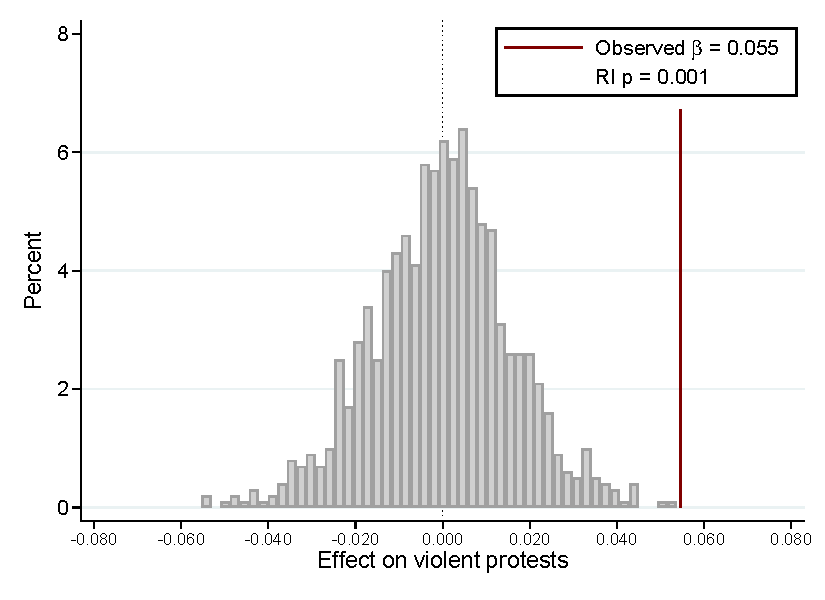
\includegraphics[width=\textwidth]{randomization_inference_hist_num_violent_MM_w30_pa.pdf}\end{subfigure}\hfill
    \begin{subfigure}{0.32\textwidth}\caption{Apex, $\pm 60$.}
        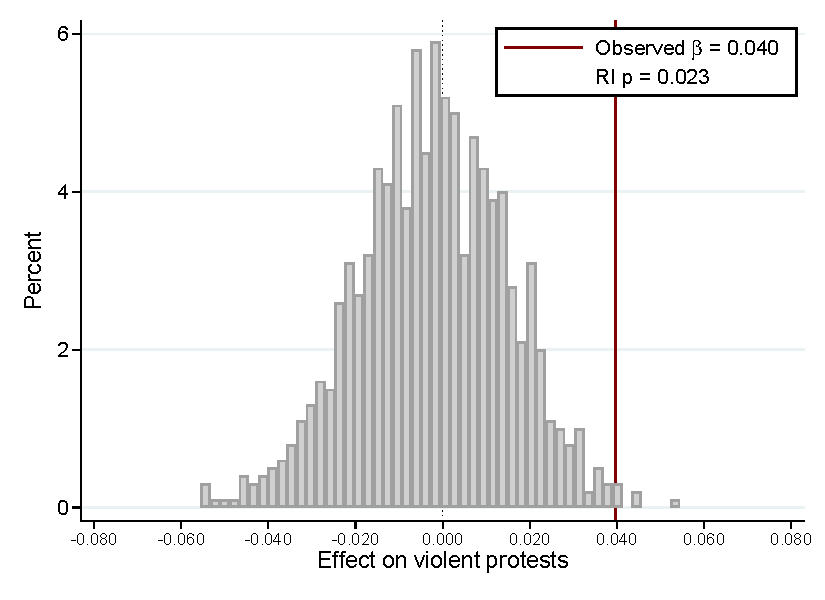
\includegraphics[width=\textwidth]{randomization_inference_hist_num_violent_MM_w60_pa.pdf}\end{subfigure}\hfill
    \begin{subfigure}{0.32\textwidth}\caption{Apex, $\pm 90$.}
        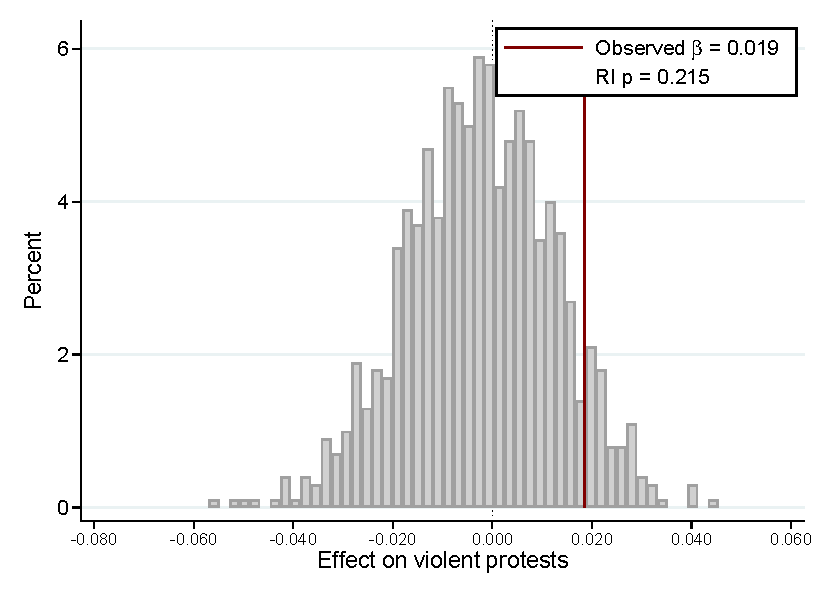
\includegraphics[width=\textwidth]{randomization_inference_hist_num_violent_MM_w90_pa.pdf}\end{subfigure} \\
    \begin{subfigure}{0.32\textwidth}\caption{Non-Apex, $\pm 30$.}
        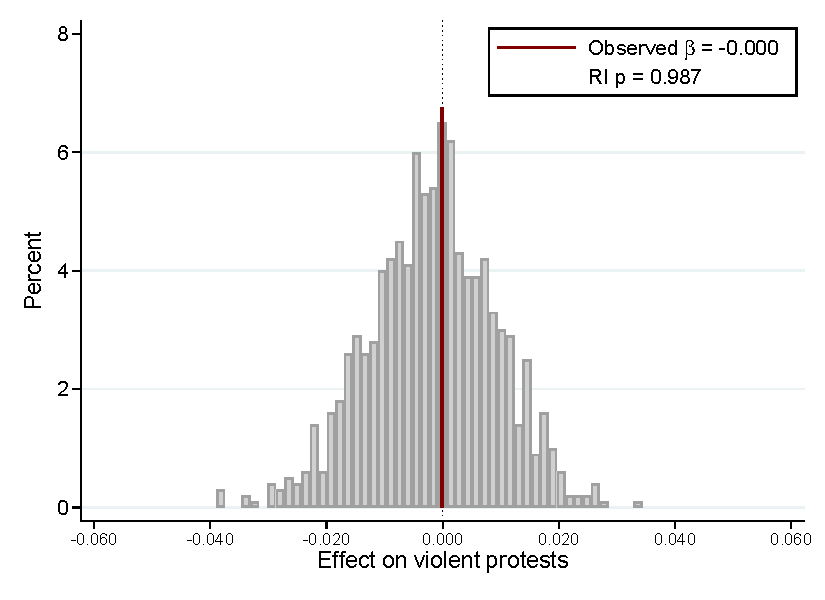
\includegraphics[width=\textwidth]{randomization_inference_hist_num_violent_MM_w30_na.pdf}\end{subfigure}\hfill
    \begin{subfigure}{0.32\textwidth}\caption{Non-Apex, $\pm 60$.}
        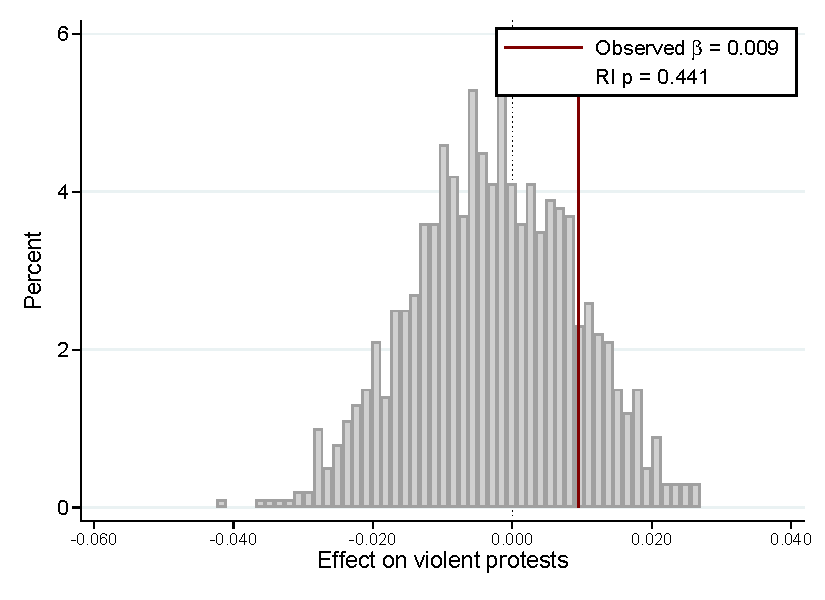
\includegraphics[width=\textwidth]{randomization_inference_hist_num_violent_MM_w60_na.pdf}\end{subfigure}\hfill
    \begin{subfigure}{0.32\textwidth}\caption{Non-Apex, $\pm 90$.}
        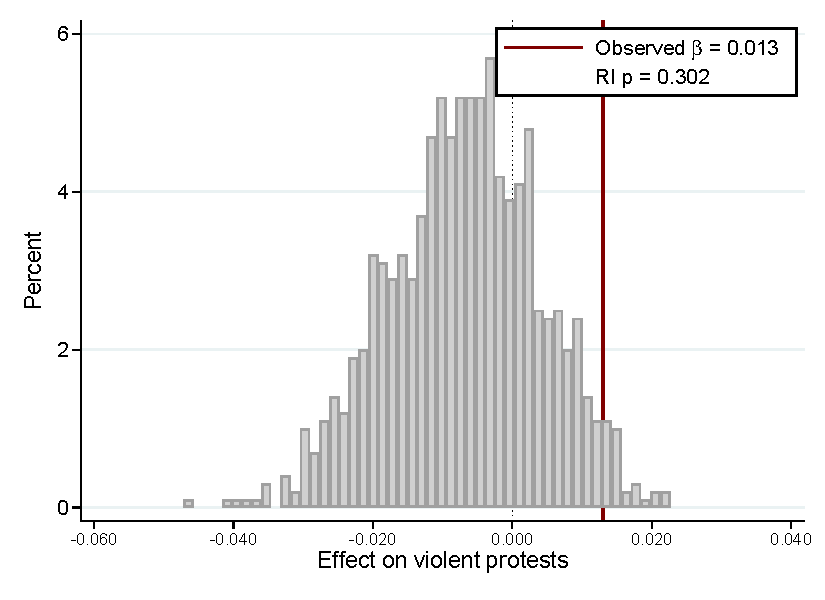
\includegraphics[width=\textwidth]{randomization_inference_hist_num_violent_MM_w90_na.pdf}\end{subfigure}
    \end{center}
    \footnotesize{Randomization inference for violent protests. Each histogram is the distribution of 1{,}000 placebo estimates of the post-scandal effect, obtained by redrawing each scandal's disclosure date at random within its own country-year and re-estimating the OLS specification on the $\pm T$ event window. Top row: Apex subsample; bottom row: Non-Apex; columns are the $\pm 30$, $\pm 60$, and $\pm 90$ day windows. The maroon vertical line (drawn on top) marks the observed $\hat\beta$ from the corresponding cell of Table~\ref{tab:uniquetocorruption}; the top-right legend reports that observed $\hat\beta$ and the two-sided randomization-inference $p$-value. Standard errors clustered at country $\times$ year $\times$ day-bin. Sample period 2008--2019; Venezuela excluded.}
\end{figure}

\begin{figure}[htb!]
    \caption{Randomization inference: peaceful protests.}
    \label{fig:sup_ri_peaceful}
    \begin{center}
    \begin{subfigure}{0.32\textwidth}\caption{Apex, $\pm 30$.}
        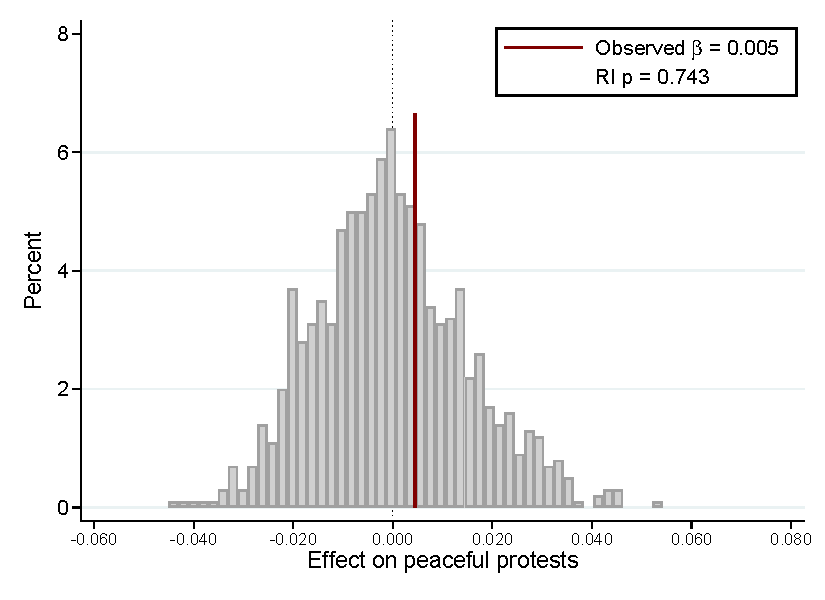
\includegraphics[width=\textwidth]{randomization_inference_hist_num_peaceful_MM_w30_pa.pdf}\end{subfigure}\hfill
    \begin{subfigure}{0.32\textwidth}\caption{Apex, $\pm 60$.}
        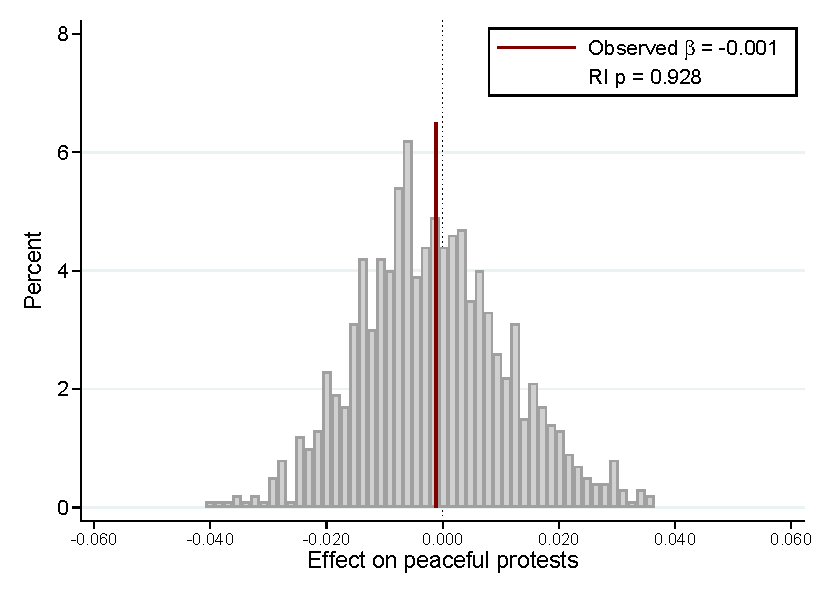
\includegraphics[width=\textwidth]{randomization_inference_hist_num_peaceful_MM_w60_pa.pdf}\end{subfigure}\hfill
    \begin{subfigure}{0.32\textwidth}\caption{Apex, $\pm 90$.}
        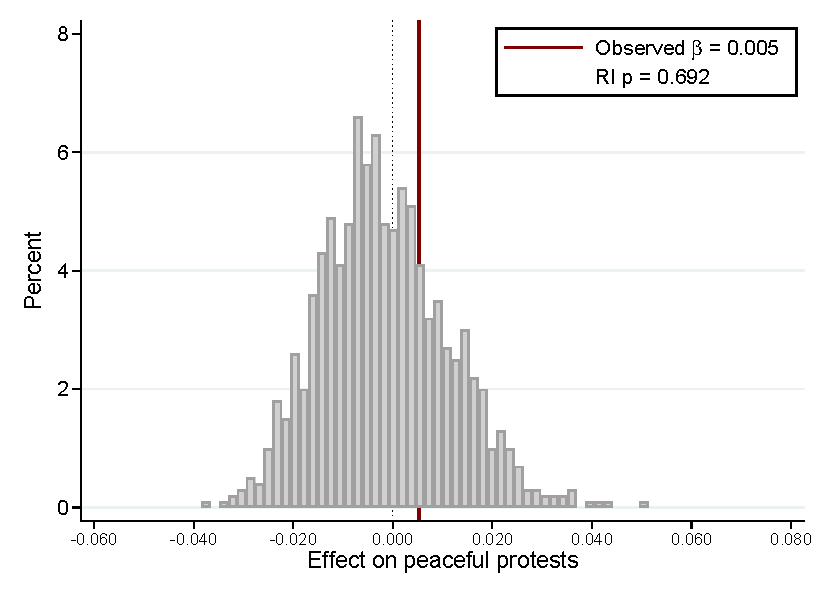
\includegraphics[width=\textwidth]{randomization_inference_hist_num_peaceful_MM_w90_pa.pdf}\end{subfigure} \\
    \begin{subfigure}{0.32\textwidth}\caption{Non-Apex, $\pm 30$.}
        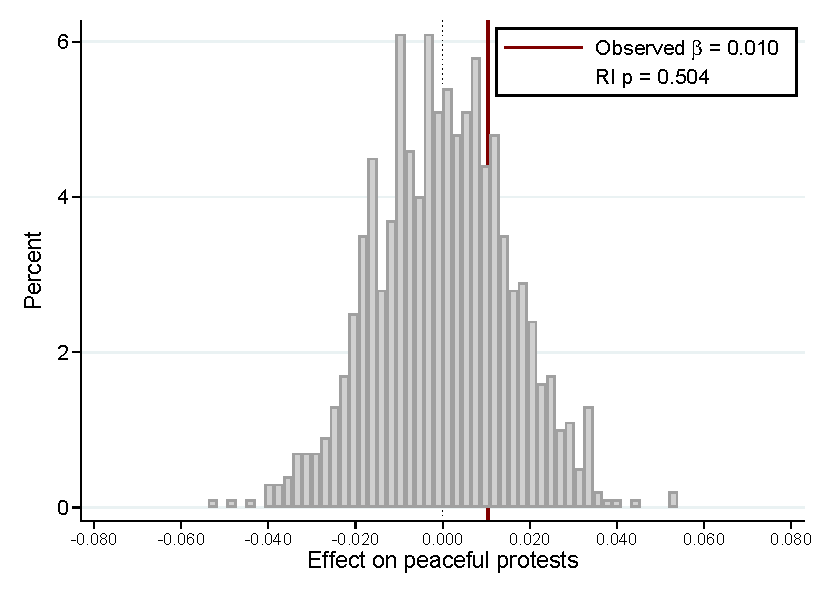
\includegraphics[width=\textwidth]{randomization_inference_hist_num_peaceful_MM_w30_na.pdf}\end{subfigure}\hfill
    \begin{subfigure}{0.32\textwidth}\caption{Non-Apex, $\pm 60$.}
        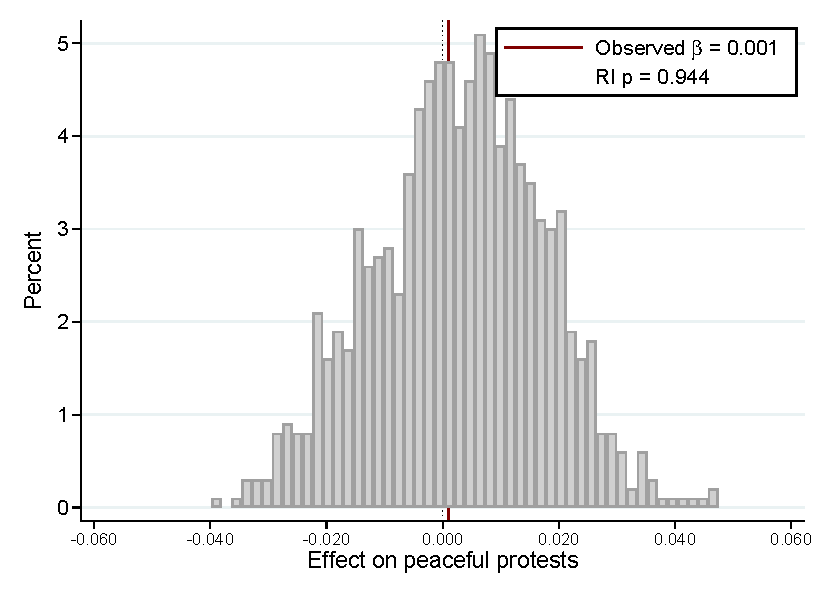
\includegraphics[width=\textwidth]{randomization_inference_hist_num_peaceful_MM_w60_na.pdf}\end{subfigure}\hfill
    \begin{subfigure}{0.32\textwidth}\caption{Non-Apex, $\pm 90$.}
        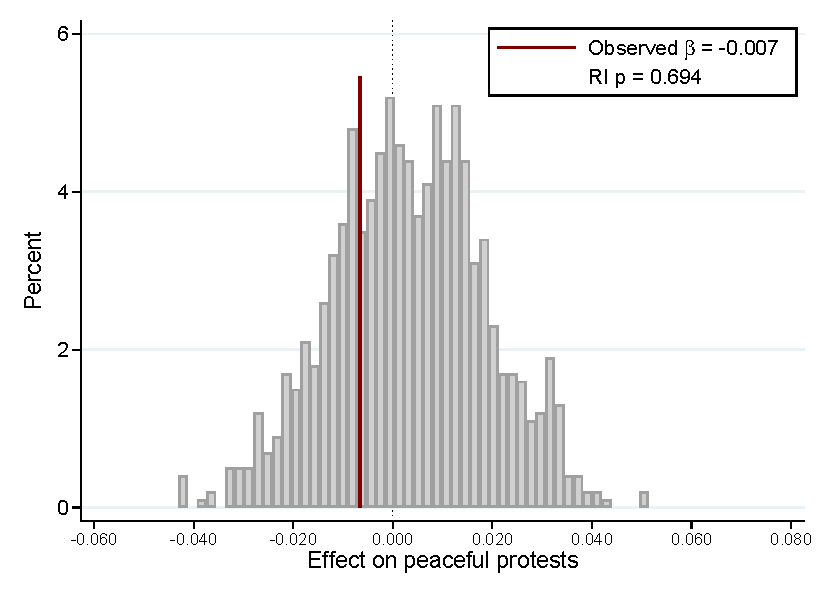
\includegraphics[width=\textwidth]{randomization_inference_hist_num_peaceful_MM_w90_na.pdf}\end{subfigure}
    \end{center}
    \footnotesize{Randomization inference for peaceful protests. Each histogram is the distribution of 1{,}000 placebo estimates of the post-scandal effect, obtained by redrawing each scandal's disclosure date at random within its own country-year and re-estimating the OLS specification on the $\pm T$ event window. Top row: Apex subsample; bottom row: Non-Apex; columns are the $\pm 30$, $\pm 60$, and $\pm 90$ day windows. The maroon vertical line (drawn on top) marks the observed $\hat\beta$ from the corresponding cell of Table~\ref{tab:main}; the top-right legend reports that observed $\hat\beta$ and the two-sided randomization-inference $p$-value. Standard errors clustered at country $\times$ year $\times$ day-bin. Sample period 2008--2019; Venezuela excluded.}
\end{figure}

% ---------------------------------------------------------------------
\clearpage
\section{Regression discontinuity in event time}\label{sup:rd}

An alternative to the event-study and difference-in-differences designs treats the scandal disclosure as a \emph{regression discontinuity in time}: the running variable is the number of days since the scandal ($w_{s,t}$), the cutoff is the disclosure date ($w_{s,t}=0$), and treatment is $\text{Post}_{st}=\mathbf{1}\{w_{s,t}\ge 0\}$. A polynomial in the running variable, allowed to differ on each side of the cutoff, models the smooth pre- and post-scandal trend; the discontinuity at $0$ is the immediate effect of disclosure, net of that trend. This handles the incoming pre-scandal trend transparently and needs none of the staggered-DiD machinery.

\autoref{tab:sup_rd_time} reports the estimated jump for the apex and non-apex subsamples, on violent and peaceful protests, for bandwidths $h\in\{30,60,90\}$ days and local-linear and local-quadratic polynomials. The local-linear estimate---the standard, and preferred over higher-order polynomials---shows a clear positive discontinuity in violent protests for apex scandals (0.034 at $h=30$, 0.067 at $h=60$) and no discontinuity for non-apex scandals or on the peaceful margin. \autoref{fig:sup_rd_time} plots the two violent-protest discontinuities: for apex scandals the residualised protest count jumps sharply upward at disclosure, whereas for non-apex scandals the fit is continuous through the cutoff. Reassuringly, the apex pre-scandal trend is, if anything, \emph{downward}, so the upward jump is not an artefact of a rising pre-trend.

\begin{table}[htb!]
    \caption{Regression discontinuity in event time: jump at disclosure.}
    \label{tab:sup_rd_time}
    \begin{center}
        \scriptsize{{
\def\sym#1{\ifmmode^{#1}\else\(^{#1}\)\fi}
\begin{tabular}{ll*{6}{c}}
\toprule
 & & \multicolumn{3}{c}{Violent Protests} & \multicolumn{3}{c}{Peaceful Protests} \\
\cmidrule(lr){3-5}\cmidrule(lr){6-8}
 & & \ensuremath{h=30} & \ensuremath{h=60} & \ensuremath{h=90} & \ensuremath{h=30} & \ensuremath{h=60} & \ensuremath{h=90} \\
\midrule
\multicolumn{8}{l}{\textit{Apex}}\\
Local linear & & 0.034 & 0.066\sym{***} & 0.056\sym{***} & 0.008 & 0.008 & 0.000 \\
 & & (0.022) & (0.018) & (0.016) & (0.018) & (0.016) & (0.014) \\
Local quadratic & & 0.038 & 0.024 & 0.067\sym{***} & 0.009 & 0.000 & 0.012 \\
 & & (0.032) & (0.024) & (0.024) & (0.022) & (0.022) & (0.021) \\
Nonparametric & & 0.029 & 0.031 & 0.030 & -0.002 & 0.004 & 0.006 \\
 & & (0.031) & (0.029) & (0.029) & (0.021) & (0.021) & (0.021) \\
\addlinespace
\multicolumn{2}{l}{MSE-optimal bandwidth (days)} & 13.3 & 23.5 & 28.3 & 10.5 & 19.7 & 36.3 \\
\multicolumn{2}{l}{Effective observations} & 1,701 & 2,961 & 3,591 & 1,323 & 2,457 & 4,599 \\
\multicolumn{2}{l}{Observations} & 3,843 & 7,623 & 11,403 & 3,843 & 7,623 & 11,403 \\
\multicolumn{2}{l}{Number of scandals} & 63 & 63 & 63 & 63 & 63 & 63 \\
\multicolumn{2}{l}{Mean (pre-scandal)} & 0.028 & 0.037 & 0.045 & 0.015 & 0.019 & 0.021 \\
\midrule
\multicolumn{8}{l}{\textit{Non-Apex}}\\
Local linear & & 0.004 & -0.005 & -0.001 & -0.012 & 0.010 & 0.007 \\
 & & (0.014) & (0.008) & (0.010) & (0.022) & (0.020) & (0.021) \\
Local quadratic & & 0.013 & 0.006 & -0.005 & -0.013 & -0.011 & 0.003 \\
 & & (0.020) & (0.016) & (0.014) & (0.025) & (0.031) & (0.031) \\
Nonparametric & & 0.012 & 0.008 & 0.007 & -0.010 & -0.013 & -0.012 \\
 & & (0.016) & (0.017) & (0.018) & (0.023) & (0.030) & (0.033) \\
\addlinespace
\multicolumn{2}{l}{MSE-optimal bandwidth (days)} & 15.6 & 28.7 & 29.8 & 15.2 & 32.0 & 37.7 \\
\multicolumn{2}{l}{Effective observations} & 3,503 & 6,441 & 6,667 & 3,503 & 7,119 & 8,475 \\
\multicolumn{2}{l}{Observations} & 6,893 & 13,673 & 20,453 & 6,893 & 13,673 & 20,453 \\
\multicolumn{2}{l}{Number of scandals} & 113 & 113 & 113 & 113 & 113 & 113 \\
\multicolumn{2}{l}{Mean (pre-scandal)} & 0.017 & 0.012 & 0.012 & 0.075 & 0.076 & 0.076 \\
\bottomrule
\end{tabular}
}
}
    \end{center}
    \footnotesize{Estimated discontinuity ($\tau$, standard error in parentheses) in the daily protest count at the disclosure cutoff ($w_{s,t}=0$), from $Y_{c(s)t} = \tau\,\text{Post}_{st} + f(w_{s,t}) + \text{Post}_{st}\cdot g(w_{s,t}) + \alpha_d + \lambda_m + \theta_{cy} + \varepsilon_{c(s)t}$, where the polynomials $f,g$ are local-linear or local-quadratic in the running variable and, the running variable being centred at $0$, the coefficient on $\text{Post}$ is exactly the jump at the cutoff. The ``Nonparametric'' rows instead report a local-polynomial estimate (\texttt{rdrobust}: MSE-optimal data-driven bandwidth, triangular kernel) computed within the $\pm h$ window on the fixed-effect-residualised outcome. Estimated separately on the apex and non-apex subsamples, on violent and peaceful protest counts, at bandwidths/windows $h\in\{30,60,90\}$ days. The foot of each panel reports the MSE-optimal bandwidth and the effective (in-bandwidth) observations for the nonparametric estimate, the number of observations and distinct scandals entering each column, and the mean of the outcome in the pre-scandal days ($w_{s,t}<0$). All specifications include country-by-year, month-of-year, and day-of-week fixed effects; standard errors clustered at the country $\times$ year $\times$ day-bin level. Sample period 2008--2019; Venezuela excluded. Significance: $^{*}$ $p<0.1$, $^{**}$ $p<0.05$, $^{***}$ $p<0.01$.}
\end{table}

\begin{figure}[htb!]
    \caption{Regression discontinuity in event time, violent protests, at $h=30/60/90$-day bandwidths.}
    \label{fig:sup_rd_time}
    \begin{center}
    \begin{subfigure}{0.45\textwidth}\caption{Apex, $h=30$.}
        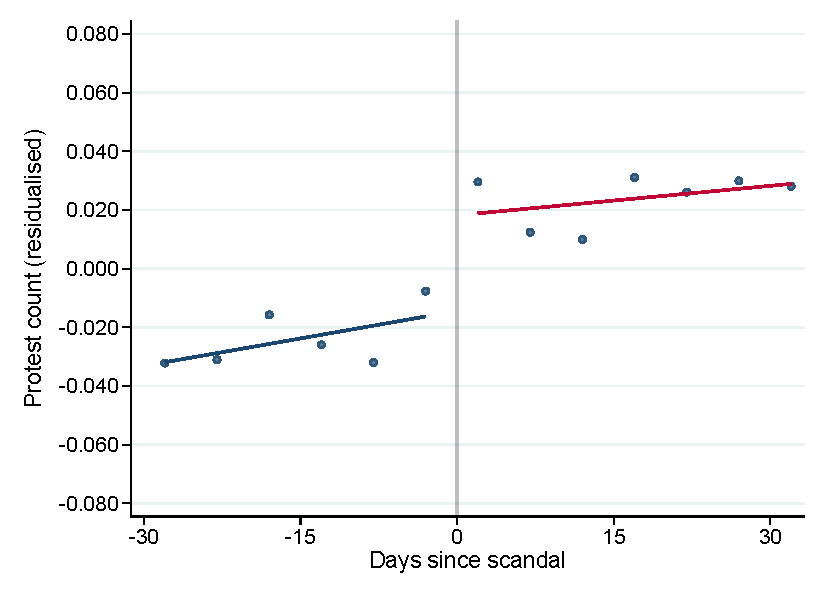
\includegraphics[width=\textwidth]{rd_time_num_violent_MM_pa_h30.pdf}\end{subfigure}\hfill
    \begin{subfigure}{0.45\textwidth}\caption{Non-Apex, $h=30$.}
        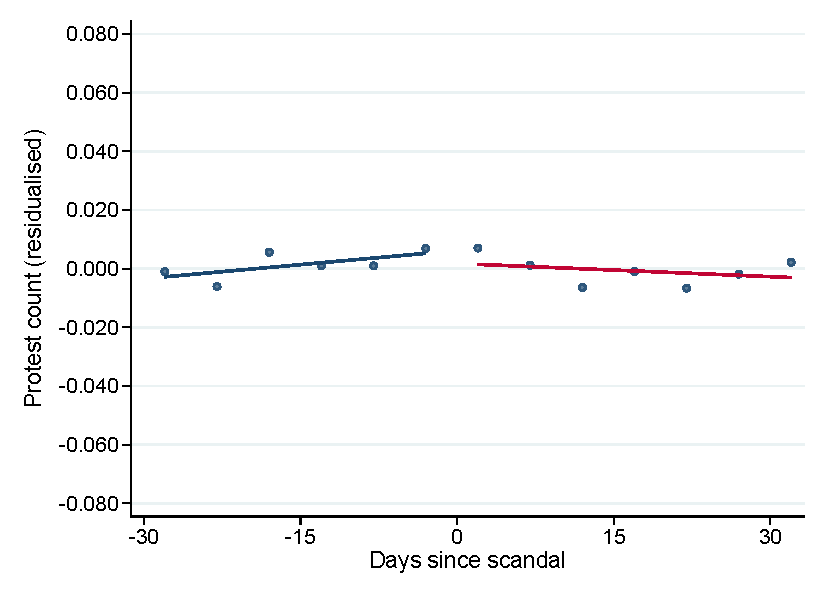
\includegraphics[width=\textwidth]{rd_time_num_violent_MM_na_h30.pdf}\end{subfigure}

    \begin{subfigure}{0.45\textwidth}\caption{Apex, $h=60$.}
        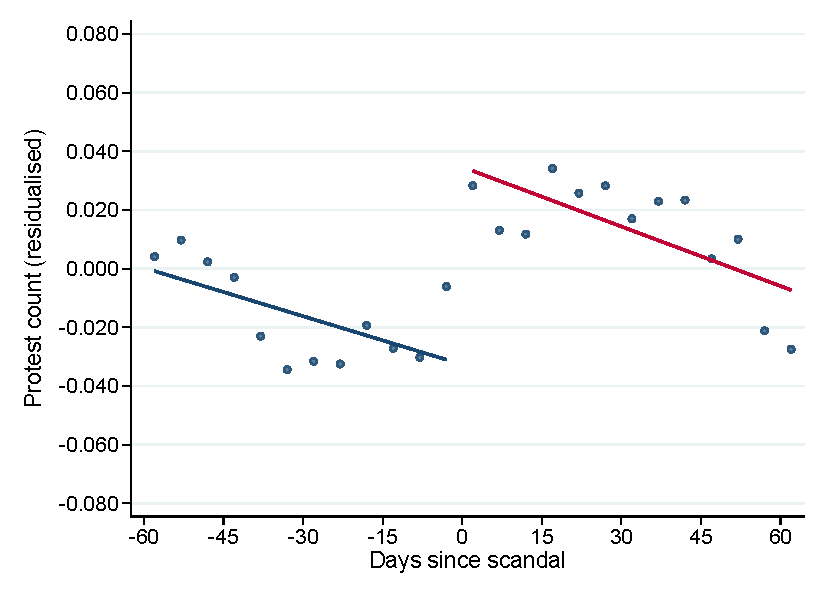
\includegraphics[width=\textwidth]{rd_time_num_violent_MM_pa_h60.pdf}\end{subfigure}\hfill
    \begin{subfigure}{0.45\textwidth}\caption{Non-Apex, $h=60$.}
        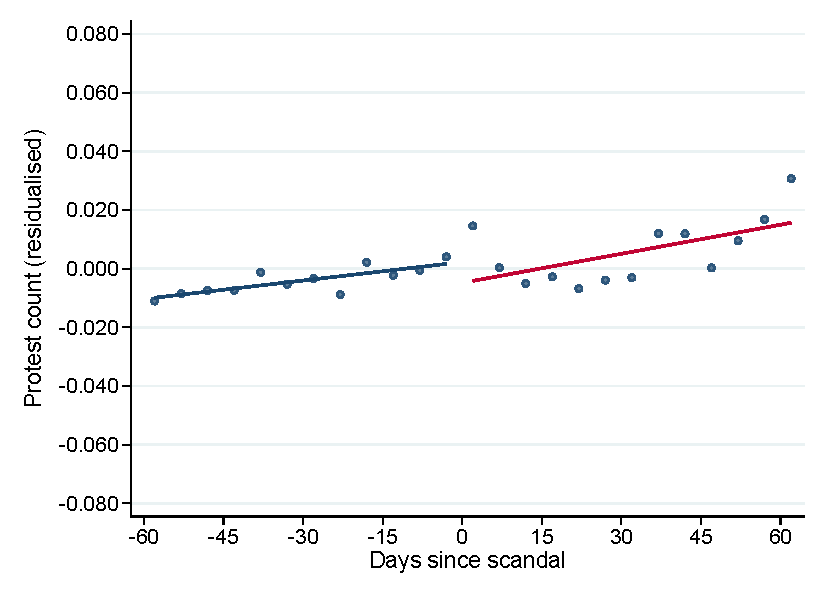
\includegraphics[width=\textwidth]{rd_time_num_violent_MM_na_h60.pdf}\end{subfigure}

    \begin{subfigure}{0.45\textwidth}\caption{Apex, $h=90$.}
        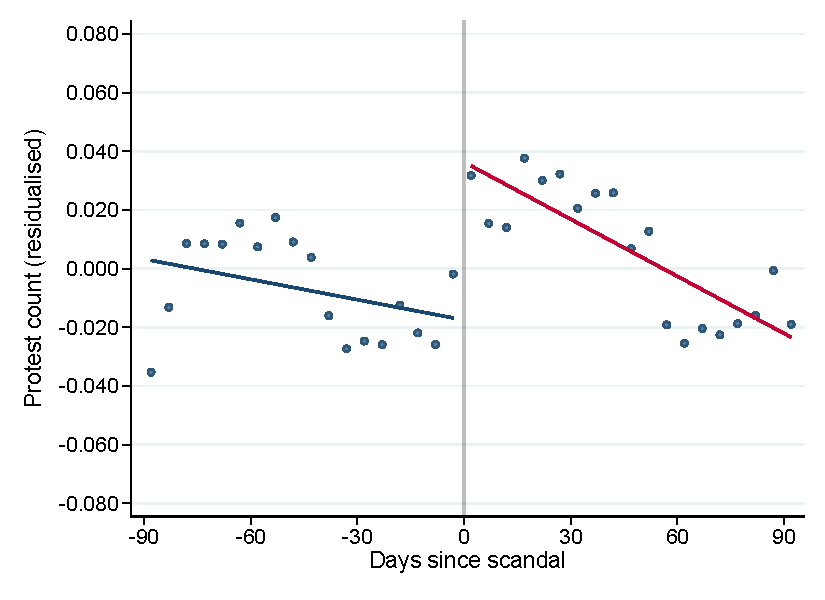
\includegraphics[width=\textwidth]{rd_time_num_violent_MM_pa_h90.pdf}\end{subfigure}\hfill
    \begin{subfigure}{0.45\textwidth}\caption{Non-Apex, $h=90$.}
        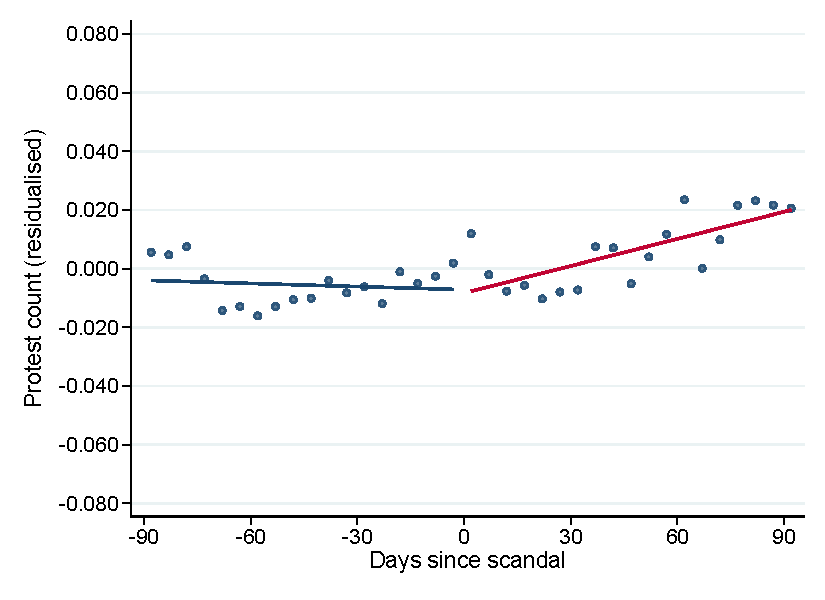
\includegraphics[width=\textwidth]{rd_time_num_violent_MM_na_h90.pdf}\end{subfigure}
    \end{center}
    \footnotesize{Binned means of the violent-protest count---residualised on the country-by-year, month-of-year, and day-of-week fixed effects---in 5-day bins of the running variable (days since scandal), with local-linear fits on each side of the disclosure cutoff, at the $h=30$ (top row), $h=60$ (middle), and $h=90$ (bottom) bandwidths. For apex scandals (left column) the count jumps upward at $w_{s,t}=0$ at every bandwidth; for non-apex scandals (right column) the fit is continuous through the cutoff. All regression-discontinuity figures share a common vertical scale so the discontinuities can be compared by eye. Sample period 2008--2019; Venezuela excluded.}
\end{figure}

\begin{figure}[htb!]
    \caption{Regression discontinuity in event time, local-quadratic fit, violent protests, at $h=30/60/90$-day bandwidths.}
    \label{fig:sup_rd_time_quad}
    \begin{center}
    \begin{subfigure}{0.45\textwidth}\caption{Apex, $h=30$.}
        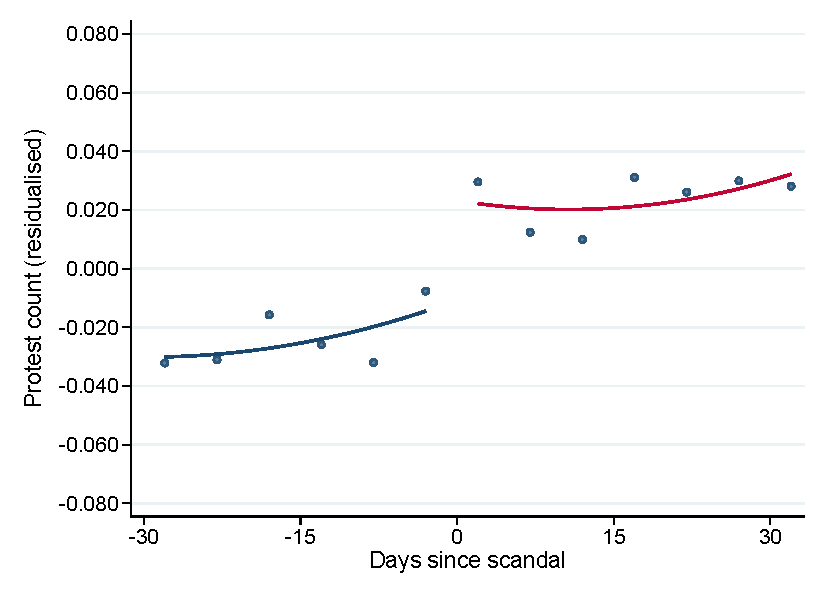
\includegraphics[width=\textwidth]{rd_time_quad_num_violent_MM_pa_h30.pdf}\end{subfigure}\hfill
    \begin{subfigure}{0.45\textwidth}\caption{Non-Apex, $h=30$.}
        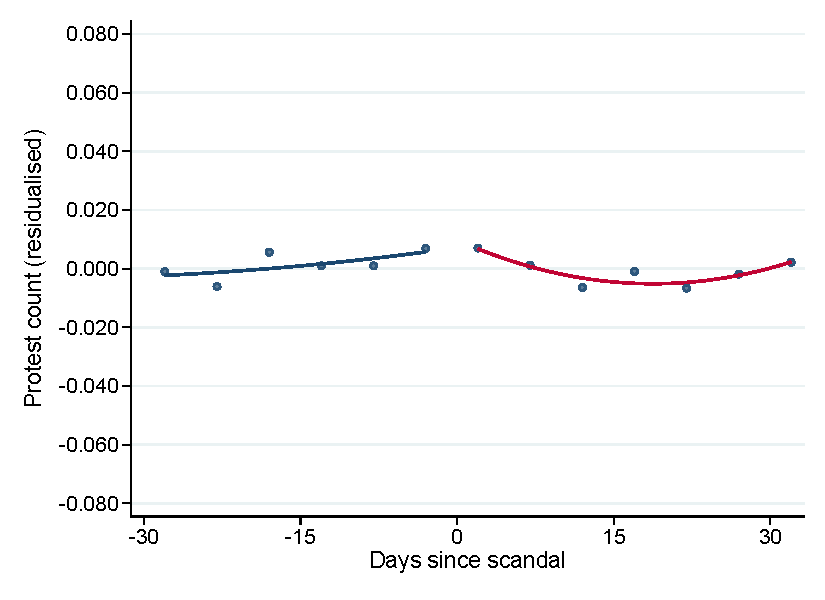
\includegraphics[width=\textwidth]{rd_time_quad_num_violent_MM_na_h30.pdf}\end{subfigure}

    \begin{subfigure}{0.45\textwidth}\caption{Apex, $h=60$.}
        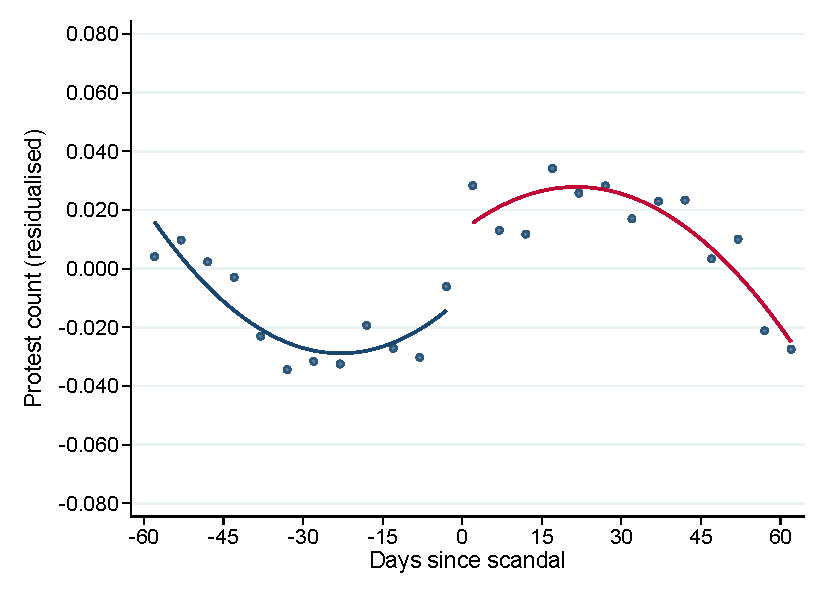
\includegraphics[width=\textwidth]{rd_time_quad_num_violent_MM_pa_h60.pdf}\end{subfigure}\hfill
    \begin{subfigure}{0.45\textwidth}\caption{Non-Apex, $h=60$.}
        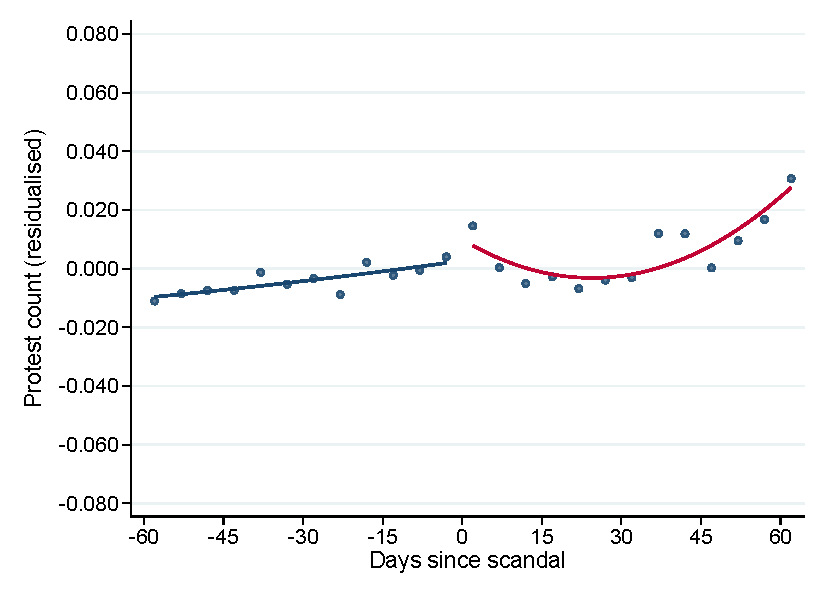
\includegraphics[width=\textwidth]{rd_time_quad_num_violent_MM_na_h60.pdf}\end{subfigure}

    \begin{subfigure}{0.45\textwidth}\caption{Apex, $h=90$.}
        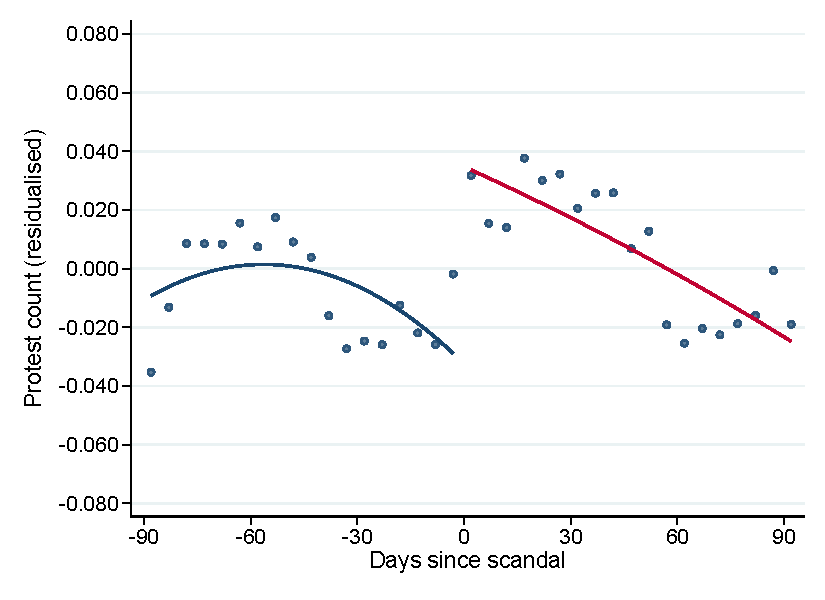
\includegraphics[width=\textwidth]{rd_time_quad_num_violent_MM_pa_h90.pdf}\end{subfigure}\hfill
    \begin{subfigure}{0.45\textwidth}\caption{Non-Apex, $h=90$.}
        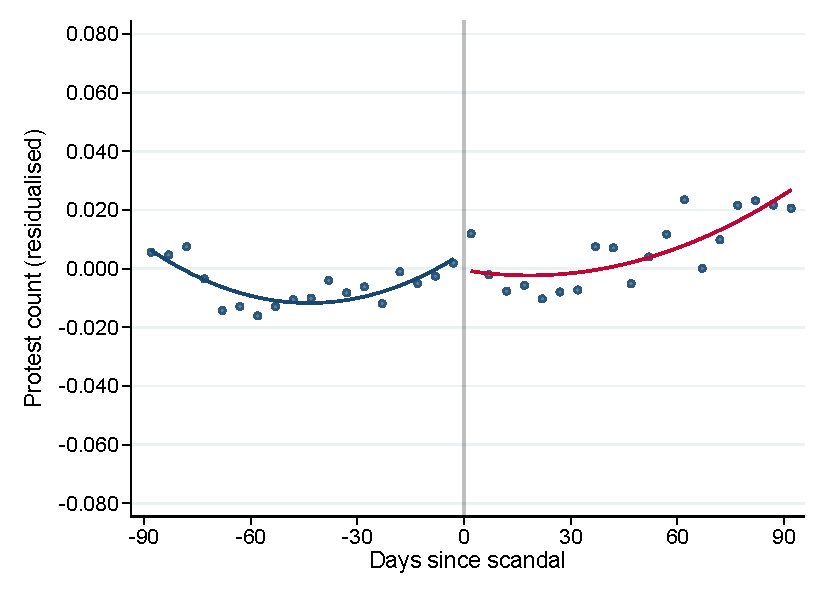
\includegraphics[width=\textwidth]{rd_time_quad_num_violent_MM_na_h90.pdf}\end{subfigure}
    \end{center}
    \footnotesize{As \autoref{fig:sup_rd_time}, but with local-\emph{quadratic} fits on each side of the disclosure cutoff, at the $h=30$ (top row), $h=60$ (middle), and $h=90$ (bottom) bandwidths. Binned means of the violent-protest count, residualised on the country-by-year, month-of-year, and day-of-week fixed effects, in 5-day bins of the running variable. For apex scandals (left column) the count jumps upward at $w_{s,t}=0$; for non-apex scandals (right column) the fit is continuous through the cutoff. Common vertical scale across all regression-discontinuity figures. Sample period 2008--2019; Venezuela excluded.}
\end{figure}

The result is robust to the polynomial choice---the local-quadratic estimates are in \autoref{tab:sup_rd_time}, and \autoref{fig:sup_rd_time_quad} plots the corresponding local-quadratic fits, which likewise jump upward at disclosure for apex scandals only---and to a fully non-parametric fit: the ``Nonparametric'' rows of \autoref{tab:sup_rd_time} report a local-polynomial regression-discontinuity estimate~\citep{calonico2014robust}, computed within each window with an MSE-optimal, data-driven bandwidth and a triangular kernel on the fixed-effect-residualised outcome, and \autoref{fig:sup_rd_time_np} shows the corresponding local-linear fits with 90\% confidence bands. The apex violent discontinuity is positive at every window; with the wider robust confidence bands it is not always individually significant, while the non-apex and peaceful estimates remain null throughout.

\begin{comment}
\begin{table}[htb!]
    \caption{Regression discontinuity in event time: non-parametric estimate.}
    \label{tab:sup_rd_time_np}
    \begin{center}
        \scriptsize{{
\def\sym#1{\ifmmode^{#1}\else\(^{#1}\)\fi}
\begin{tabular}{l*{6}{c}}
\toprule
 & \multicolumn{3}{c}{Violent Protests} & \multicolumn{3}{c}{Peaceful Protests} \\
\cmidrule(lr){2-4}\cmidrule(lr){5-7}
 & \ensuremath{h=30} & \ensuremath{h=60} & \ensuremath{h=90} & \ensuremath{h=30} & \ensuremath{h=60} & \ensuremath{h=90} \\
\midrule
Apex & 0.029 & 0.031 & 0.030 & -0.002 & 0.004 & 0.006 \\
  & (0.031) & (0.029) & (0.029) & (0.021) & (0.021) & (0.021) \\
Non-Apex & 0.002 & -0.000 & -0.001 & -0.007 & -0.012 & -0.011 \\
  & (0.013) & (0.015) & (0.017) & (0.023) & (0.031) & (0.034) \\
\bottomrule
\end{tabular}
}
}
    \end{center}
    \footnotesize{Local-polynomial (local-linear) regression-discontinuity estimate of the jump in the daily protest count at the disclosure cutoff, computed with \texttt{rdrobust}~\citep{calonico2014robust}: triangular kernel, on the outcome residualised on the country-by-year, month-of-year, and day-of-week fixed effects. Estimation is restricted to a $\pm30$, $\pm60$, or $\pm90$ day window (columns $h=30/60/90$), and within each window \texttt{rdrobust} selects its own MSE-optimal data-driven bandwidth. Standard errors (in parentheses), clustered at the country $\times$ year $\times$ day-bin level, are the robust bias-corrected standard errors. Estimated separately on the apex and non-apex subsamples, on violent and peaceful protest counts. Sample period 2008--2019; Venezuela excluded. Significance: $^{*}$ $p<0.1$, $^{**}$ $p<0.05$, $^{***}$ $p<0.01$.}
\end{table}
\end{comment}

\begin{figure}[htb!]
    \caption{Regression discontinuity in event time, non-parametric fit, violent protests, at $\pm30/60/90$-day windows.}
    \label{fig:sup_rd_time_np}
    \begin{center}
    \begin{subfigure}{0.45\textwidth}\caption{Apex, $\pm30$.}
        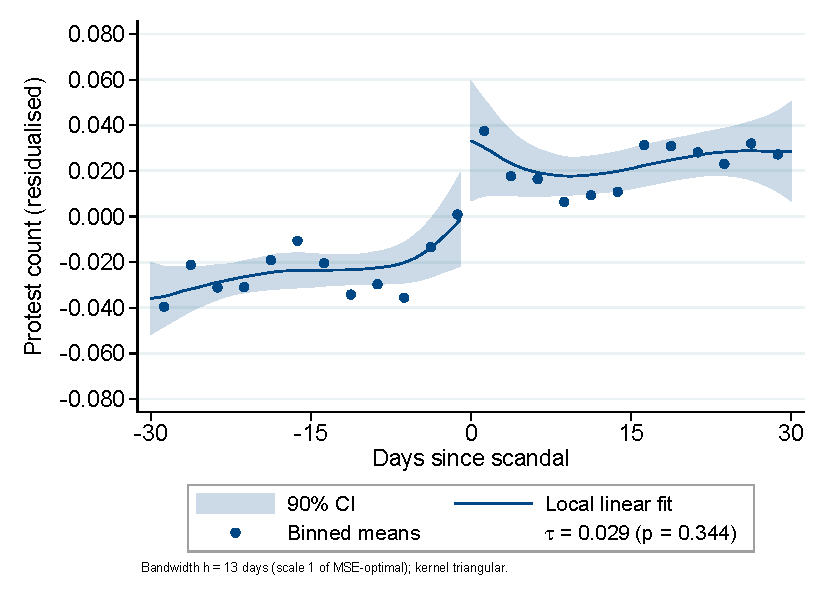
\includegraphics[width=\textwidth]{rd_time_np_num_violent_MM_pa_h30.pdf}\end{subfigure}\hfill
    \begin{subfigure}{0.45\textwidth}\caption{Non-Apex, $\pm30$.}
        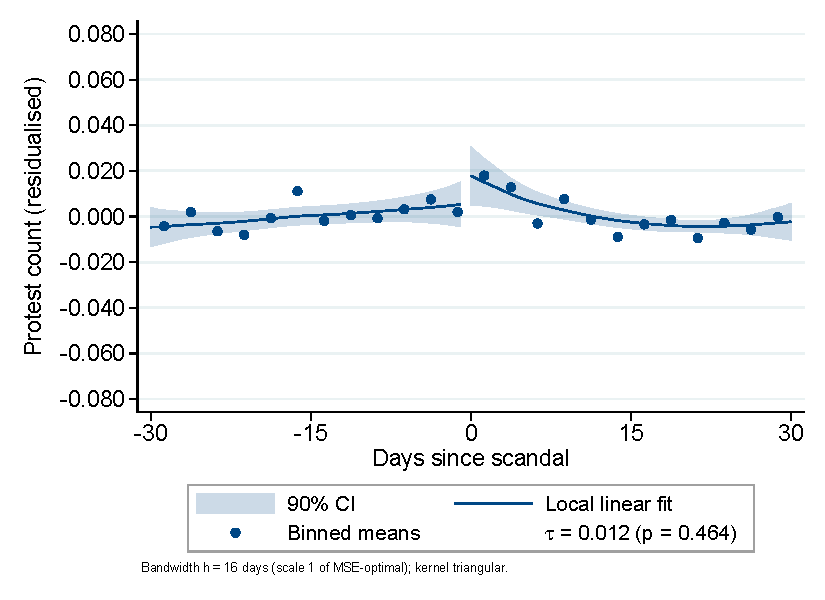
\includegraphics[width=\textwidth]{rd_time_np_num_violent_MM_na_h30.pdf}\end{subfigure}

    \begin{subfigure}{0.45\textwidth}\caption{Apex, $\pm60$.}
        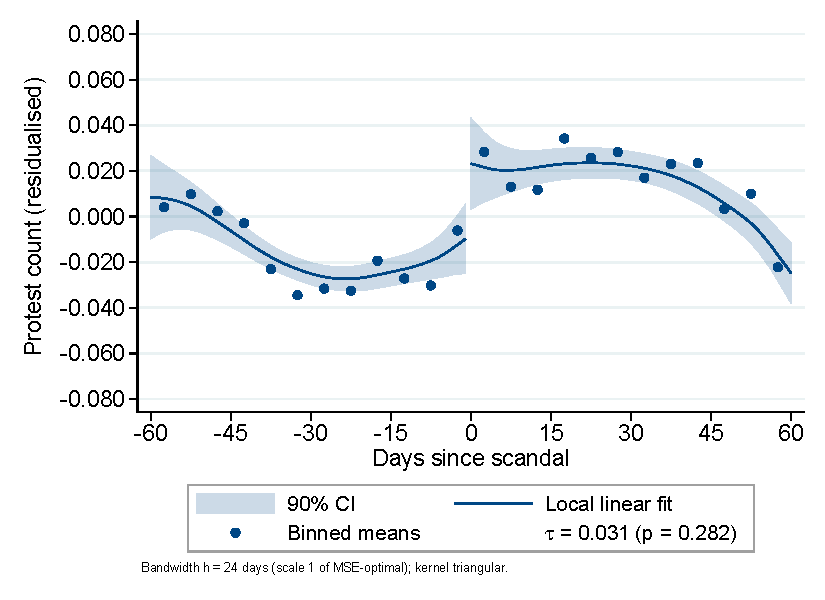
\includegraphics[width=\textwidth]{rd_time_np_num_violent_MM_pa_h60.pdf}\end{subfigure}\hfill
    \begin{subfigure}{0.45\textwidth}\caption{Non-Apex, $\pm60$.}
        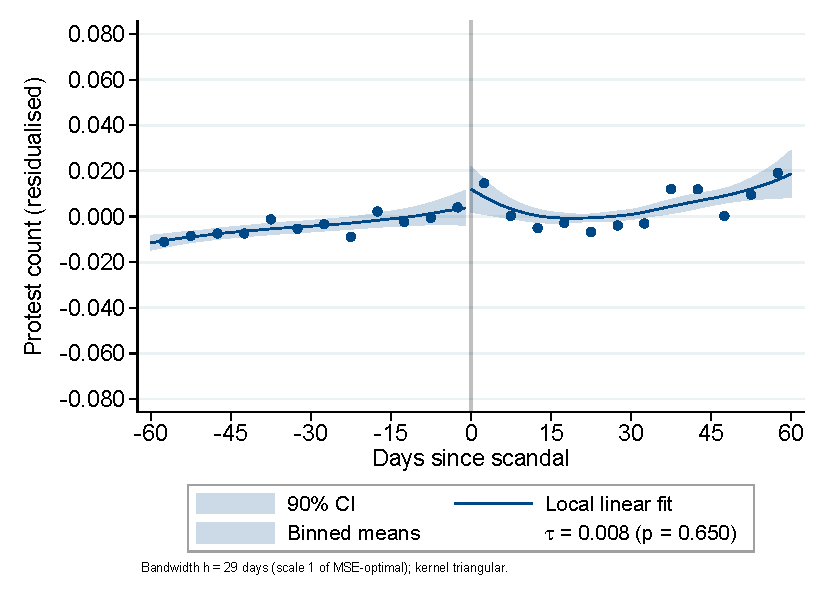
\includegraphics[width=\textwidth]{rd_time_np_num_violent_MM_na_h60.pdf}\end{subfigure}

    \begin{subfigure}{0.45\textwidth}\caption{Apex, $\pm90$.}
        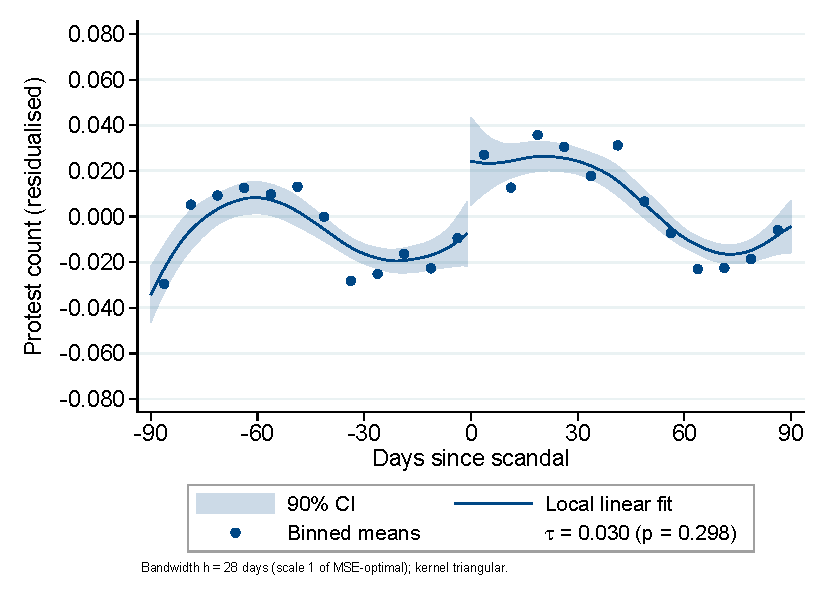
\includegraphics[width=\textwidth]{rd_time_np_num_violent_MM_pa_h90.pdf}\end{subfigure}\hfill
    \begin{subfigure}{0.45\textwidth}\caption{Non-Apex, $\pm90$.}
        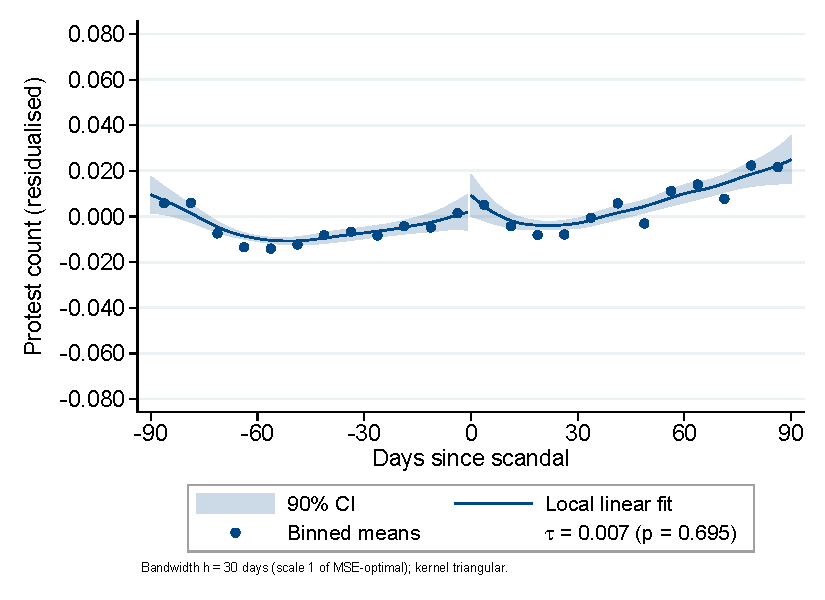
\includegraphics[width=\textwidth]{rd_time_np_num_violent_MM_na_h90.pdf}\end{subfigure}
    \end{center}
    \footnotesize{Local-linear fits (triangular kernel, MSE-optimal data-driven bandwidth) with 90\% confidence bands, and binned means (12 per side), of the violent-protest count residualised on the country-by-year, month-of-year, and day-of-week fixed effects, on each side of the disclosure cutoff. Each row restricts estimation to a $\pm30$ (top), $\pm60$ (middle), or $\pm90$ (bottom) day window, within which \texttt{rdrobust} selects its own MSE-optimal bandwidth; the legend reports the resulting discontinuity estimate $\tau$ and its $p$-value. Apex scandals in the left column, non-apex in the right. Common vertical scale across all regression-discontinuity figures. Sample period 2008--2019; Venezuela excluded.}
\end{figure}

% ---------------------------------------------------------------------
\clearpage
% =====================================================================
% WE COMMENTED THESE OUT BECAUSE THE TIGHTER COMPARISON IS ACHIEVED BY
% SUBSETTING THE ESTIMATION SAMPLE TO APEX SCANDALS AND THEN RUNNING THE
% REGRESSION ON THAT SAMPLE; THESE REGRESSIONS USE THE FULL APEX AND
% NON-APEX SAMPLE SO THE CONTROL GROUP IS DIFFERENT
% =====================================================================
\begin{comment}
\section{Pooled event studies at other window widths}\label{sup:es_pooled_windows}

\autoref{fig:dynamics} in the main text reports the pooled event study---the apex and non-apex event-time paths estimated jointly (\autoref{eq:dynamics}), directly comparable to the aggregate contrast in \autoref{tab:interaction}---at the $\pm 60$-day window. Figures~\ref{fig:sup_es_pooled_w30}--\ref{fig:sup_es_pooled_w120} report the same specification at the $\pm 30$, $\pm 90$, and $\pm 120$-day windows. Within each figure the violent and peaceful panels share a common y-axis.

\begin{figure}[htb!]
    \caption{Pooled event study, $\pm 30$-day window (15-day bins).}
    \label{fig:sup_es_pooled_w30}
    \begin{center}
    \begin{subfigure}{0.48\textwidth}\caption{Violent protests.}
        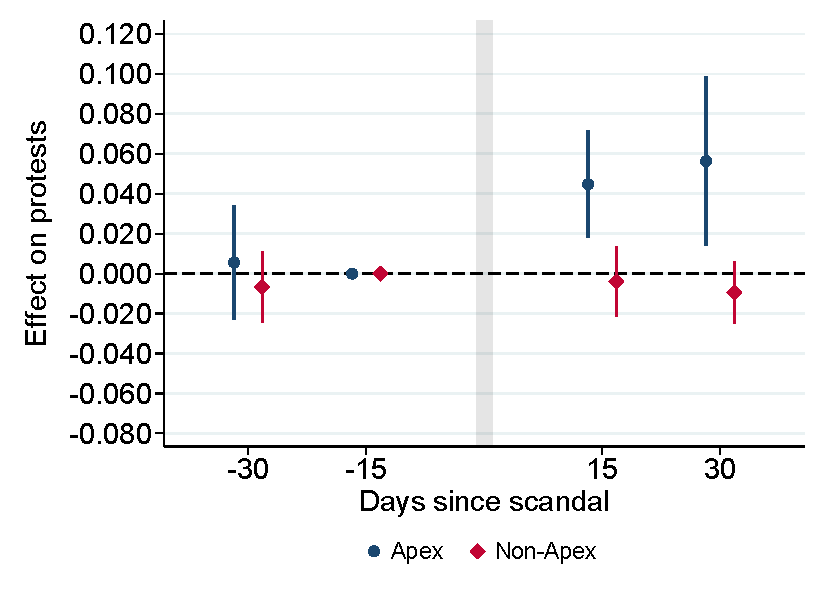
\includegraphics[width=\textwidth]{es_pooled_num_violent_MM_w30_b15_ols_90ci.pdf}\end{subfigure}\hfill
    \begin{subfigure}{0.48\textwidth}\caption{Peaceful protests.}
        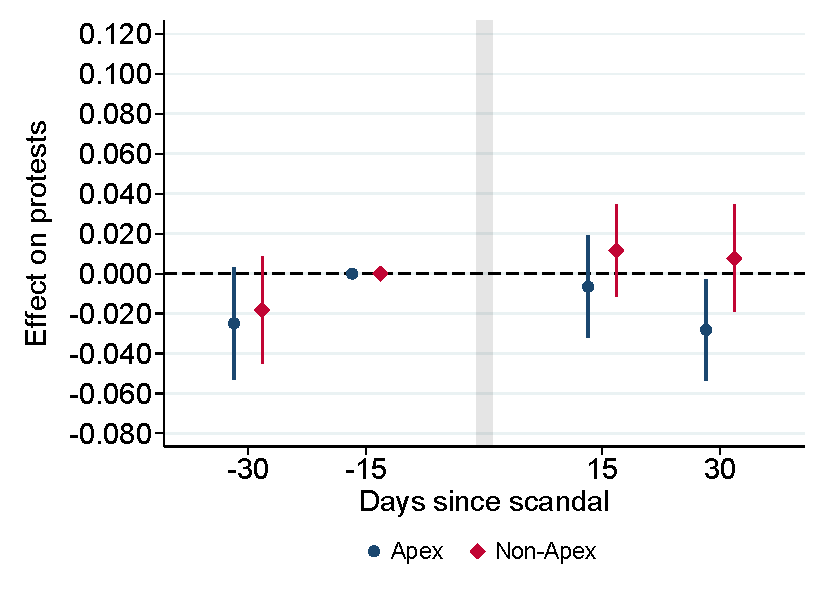
\includegraphics[width=\textwidth]{es_pooled_num_peaceful_MM_w30_b15_ols_90ci.pdf}\end{subfigure}
    \end{center}
    \footnotesize{Pooled event study (\autoref{eq:dynamics}): event-time coefficients for the Apex (navy circles) and Non-Apex (maroon diamonds) groups, estimated jointly on the pooled sample, at the $\pm 30$-day window. The bin immediately preceding disclosure ($w_{s,t}\in[-15,-1]$) is the omitted reference for each group. Vertical bars are 90\% confidence intervals; SE clustered at country $\times$ year $\times$ day-bin. Sample period 2008--2019; Venezuela excluded.}
\end{figure}

\begin{figure}[htb!]
    \caption{Pooled event study, $\pm 90$-day window (15-day bins).}
    \label{fig:sup_es_pooled_w90}
    \begin{center}
    \begin{subfigure}{0.48\textwidth}\caption{Violent protests.}
        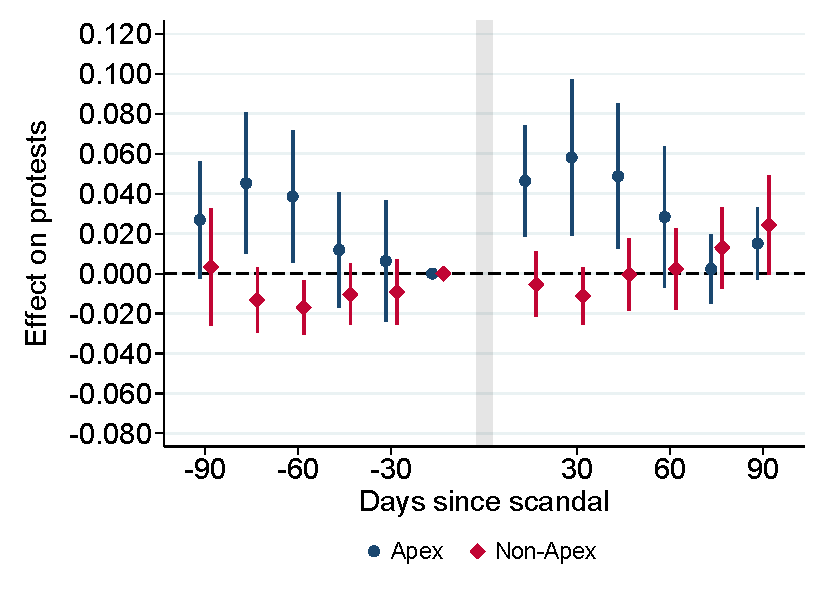
\includegraphics[width=\textwidth]{es_pooled_num_violent_MM_w90_b15_ols_90ci.pdf}\end{subfigure}\hfill
    \begin{subfigure}{0.48\textwidth}\caption{Peaceful protests.}
        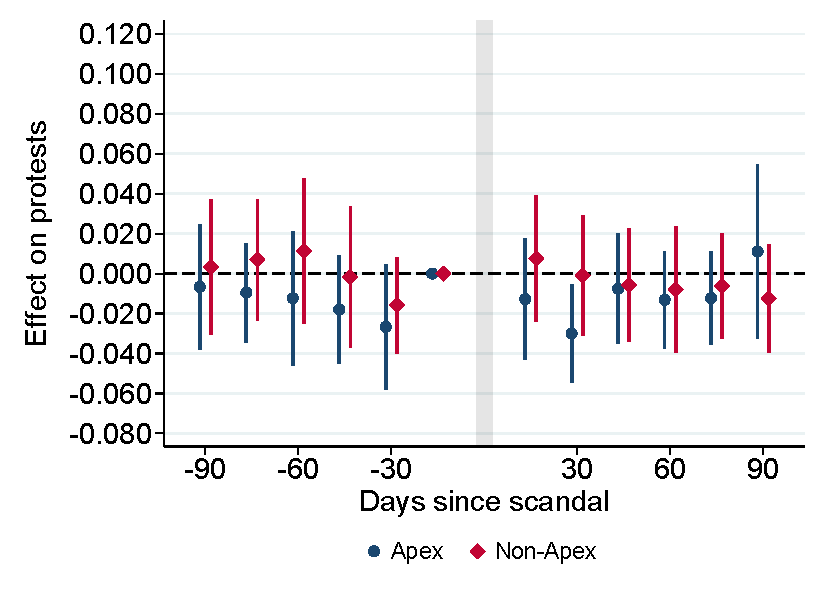
\includegraphics[width=\textwidth]{es_pooled_num_peaceful_MM_w90_b15_ols_90ci.pdf}\end{subfigure}
    \end{center}
    \footnotesize{Pooled event study (\autoref{eq:dynamics}): event-time coefficients for the Apex (navy circles) and Non-Apex (maroon diamonds) groups, estimated jointly on the pooled sample, at the $\pm 90$-day window (15-day bins). The bin immediately preceding disclosure ($w_{s,t}\in[-15,-1]$) is the omitted reference for each group. Vertical bars are 90\% confidence intervals; standard errors clustered at country $\times$ year $\times$ day-bin. Sample period 2008--2019; Venezuela excluded.}
\end{figure}

\begin{figure}[htb!]
    \caption{Pooled event study, $\pm 120$-day window (15-day bins).}
    \label{fig:sup_es_pooled_w120}
    \begin{center}
    \begin{subfigure}{0.48\textwidth}\caption{Violent protests.}
        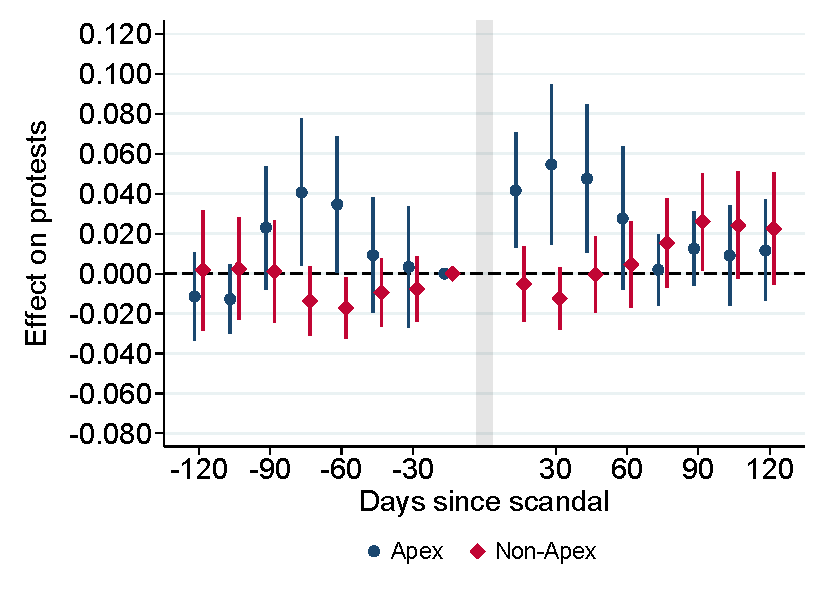
\includegraphics[width=\textwidth]{es_pooled_num_violent_MM_w120_b15_ols_90ci.pdf}\end{subfigure}\hfill
    \begin{subfigure}{0.48\textwidth}\caption{Peaceful protests.}
        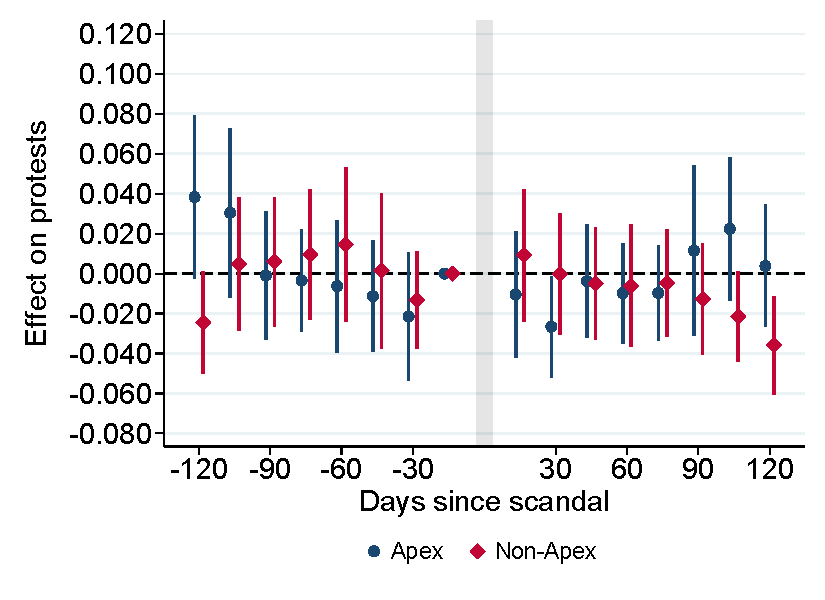
\includegraphics[width=\textwidth]{es_pooled_num_peaceful_MM_w120_b15_ols_90ci.pdf}\end{subfigure}
    \end{center}
    \footnotesize{Pooled event study (\autoref{eq:dynamics}): event-time coefficients for the Apex (navy circles) and Non-Apex (maroon diamonds) groups, estimated jointly on the pooled sample, at the $\pm 120$-day window (15-day bins). The bin immediately preceding disclosure ($w_{s,t}\in[-15,-1]$) is the omitted reference for each group. Vertical bars are 90\% confidence intervals; standard errors clustered at country $\times$ year $\times$ day-bin. Sample period 2008--2019; Venezuela excluded.}
\end{figure}

% Pooled +-60 event study (was Figure 1 in the main body; replaced there by the
% subsample version). Kept here, commented, for the reason stated at the top.
\begin{figure}[htb!]
    \caption{Pooled event study, $\pm 60$-day window (15-day bins).}
    \begin{center}
    \begin{subfigure}{0.48\textwidth}\caption{Violent protests.}
        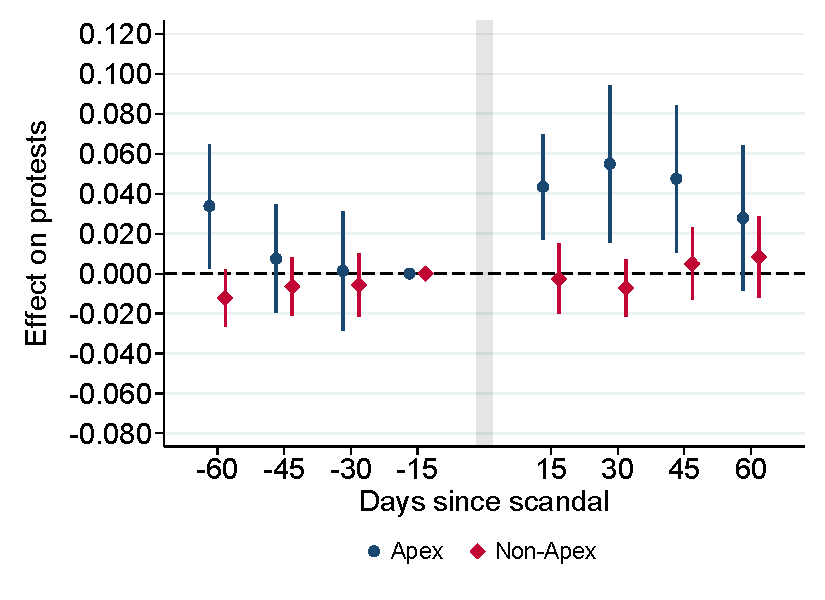
\includegraphics[width=\textwidth]{es_pooled_num_violent_MM_w60_b15_ols_90ci.pdf}\end{subfigure}\hfill
    \begin{subfigure}{0.48\textwidth}\caption{Peaceful protests.}
        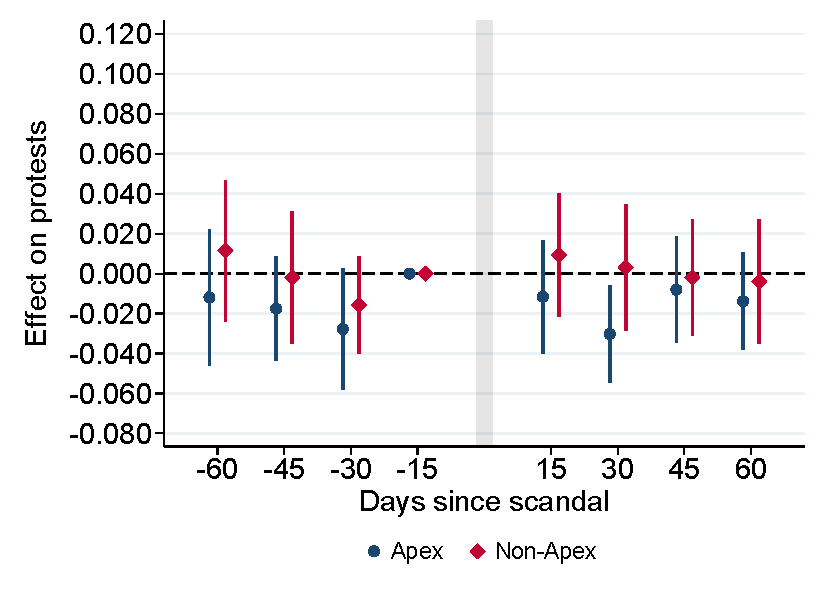
\includegraphics[width=\textwidth]{es_pooled_num_peaceful_MM_w60_b15_ols_90ci.pdf}\end{subfigure}
    \end{center}
    \footnotesize{Pooled event study: Apex (navy) and Non-Apex (maroon) event-time coefficients estimated jointly on the pooled sample, $\pm 60$-day window (15-day bins).}
\end{figure}
\end{comment}

% ---------------------------------------------------------------------
\clearpage
\section{Event studies by subsample in the $\pm30$- and $60$-day windows}\label{sup:es_windows}

\begin{figure}[htb!]
    \caption{Event studies, $\pm 30$-day window (15-day bins).}
    \label{fig:sup_es_w30}
    \begin{center}
    \begin{subfigure}{0.45\textwidth}\caption{Violent, Apex.}
        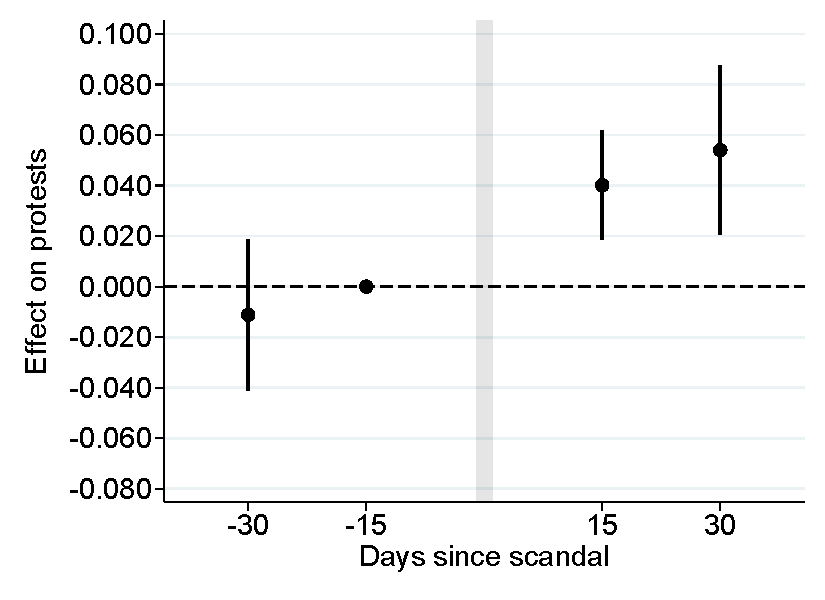
\includegraphics[width=\textwidth]{es_num_violent_MM_w30_b15_pa_ols_90ci.pdf}\end{subfigure}\hfill
    \begin{subfigure}{0.45\textwidth}\caption{Peaceful, Apex.}
        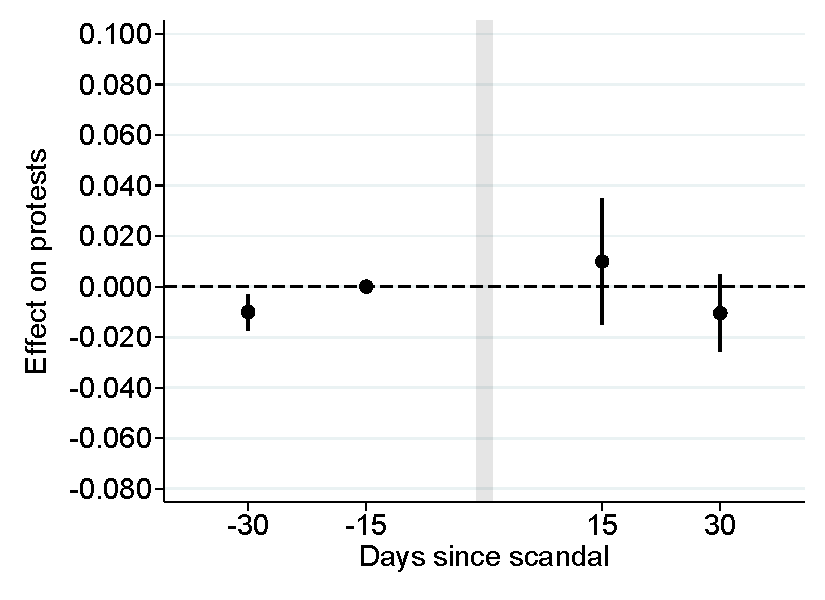
\includegraphics[width=\textwidth]{es_num_peaceful_MM_w30_b15_pa_ols_90ci.pdf}\end{subfigure} \\
    \begin{subfigure}{0.45\textwidth}\caption{Violent, Non-Apex.}
        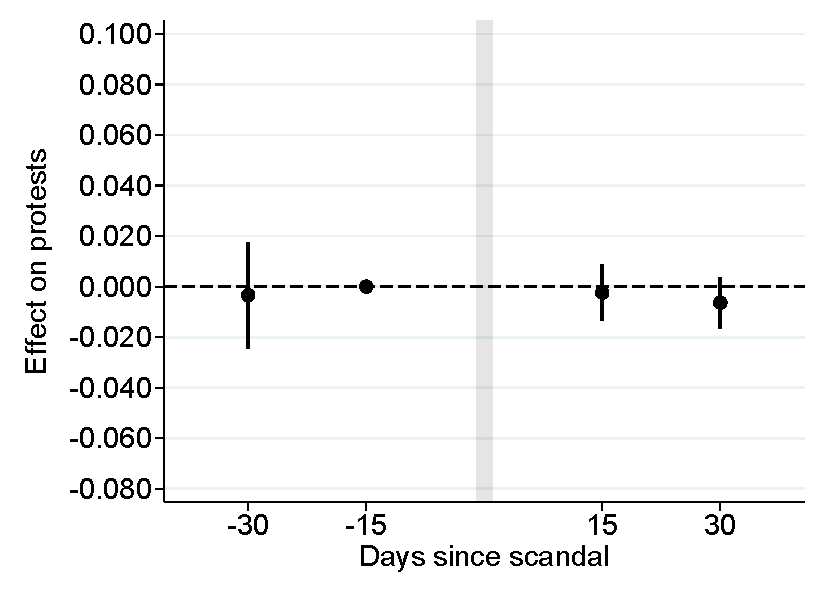
\includegraphics[width=\textwidth]{es_num_violent_MM_w30_b15_na_ols_90ci.pdf}\end{subfigure}\hfill
    \begin{subfigure}{0.45\textwidth}\caption{Peaceful, Non-Apex.}
        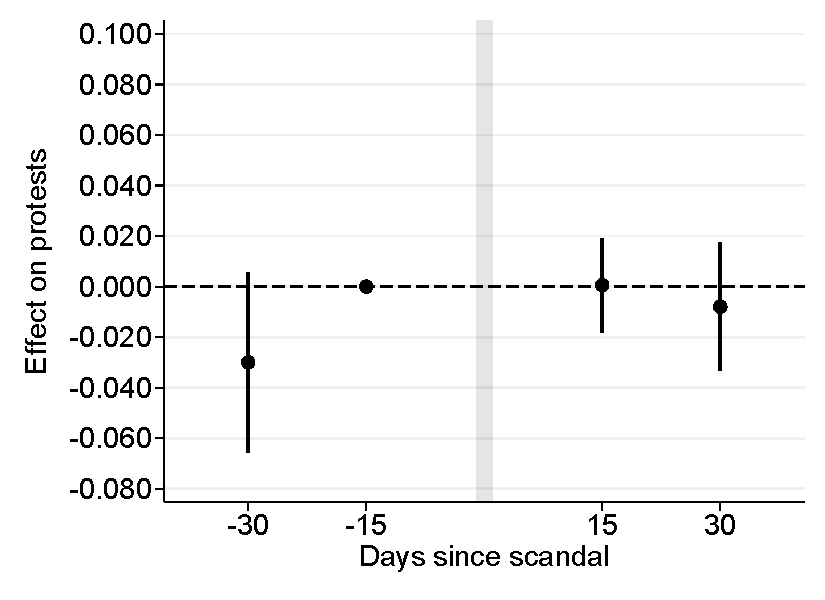
\includegraphics[width=\textwidth]{es_num_peaceful_MM_w30_b15_na_ols_90ci.pdf}\end{subfigure}
    \end{center}
    \footnotesize{OLS event study estimated separately on the Apex and Non-Apex subsamples, on 15-day event-time bin indicators over the $\pm 30$-day window (\autoref{eq:main} with the post indicator replaced by a saturated set of event-time bins). The four panels are violent and peaceful protests $\times$ Apex and Non-Apex; the reference bin (the 15 days before disclosure) is normalized to zero and shown at its position, and the faint thick vertical line marks the disclosure cutoff. All four panels share a common y-axis. Vertical bars are 90\% confidence intervals; standard errors clustered at country $\times$ year $\times$ day-bin. Sample period 2008--2019; Venezuela excluded.}
\end{figure}

% The +-60 subsample event study is now Figure~\ref{fig:dynamics} in the main body.

\begin{figure}[htb!]
    \caption{Event studies, $\pm 90$-day window (15-day bins).}
    \label{fig:sup_es_w90}
    \begin{center}
    \begin{subfigure}{0.45\textwidth}\caption{Violent, Apex.}
        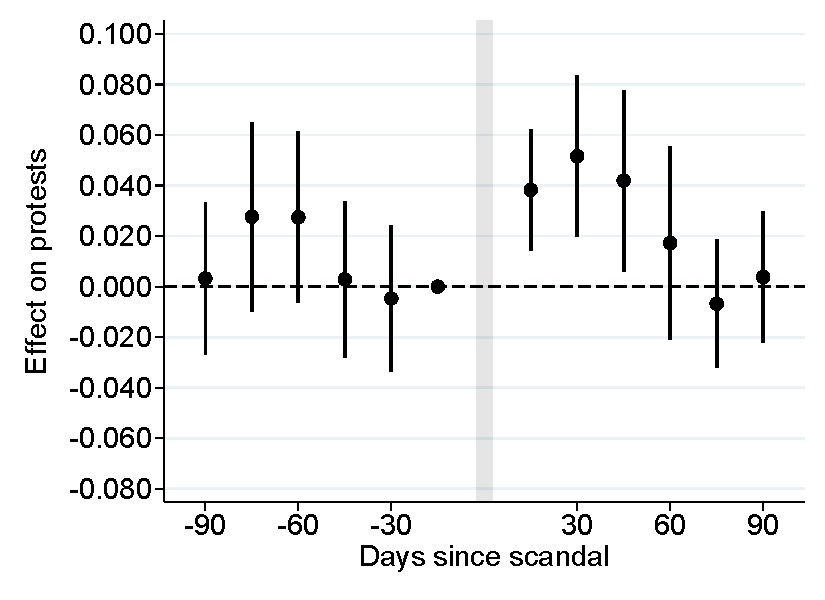
\includegraphics[width=\textwidth]{es_num_violent_MM_w90_b15_pa_ols_90ci.pdf}\end{subfigure}\hfill
    \begin{subfigure}{0.45\textwidth}\caption{Peaceful, Apex.}
        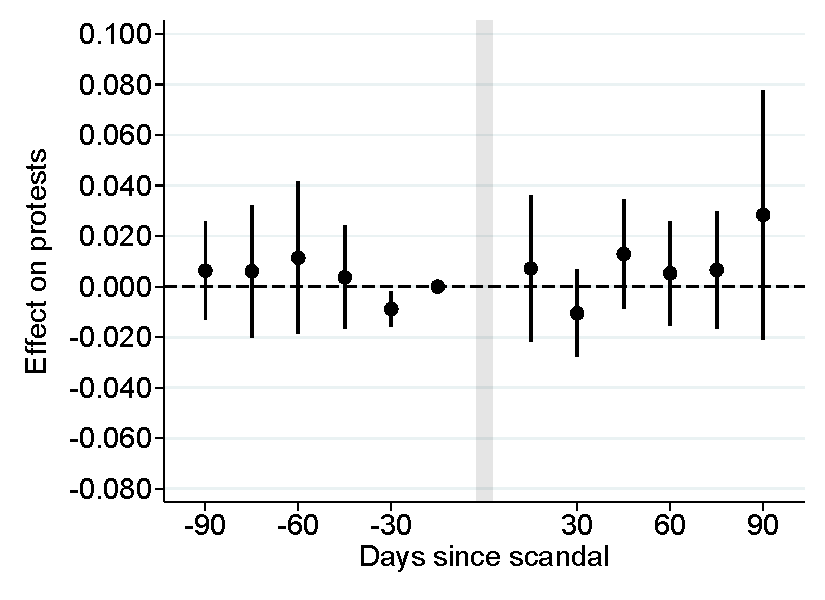
\includegraphics[width=\textwidth]{es_num_peaceful_MM_w90_b15_pa_ols_90ci.pdf}\end{subfigure} \\
    \begin{subfigure}{0.45\textwidth}\caption{Violent, Non-Apex.}
        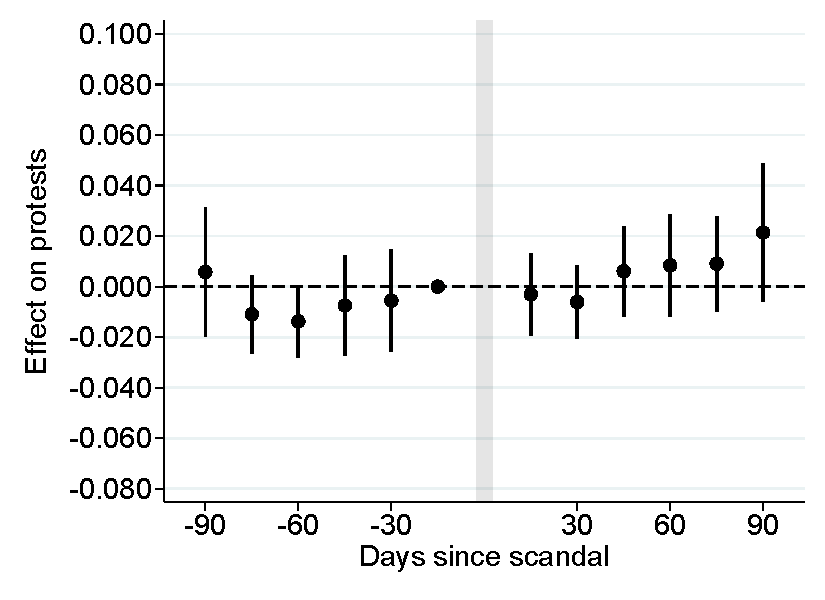
\includegraphics[width=\textwidth]{es_num_violent_MM_w90_b15_na_ols_90ci.pdf}\end{subfigure}\hfill
    \begin{subfigure}{0.45\textwidth}\caption{Peaceful, Non-Apex.}
        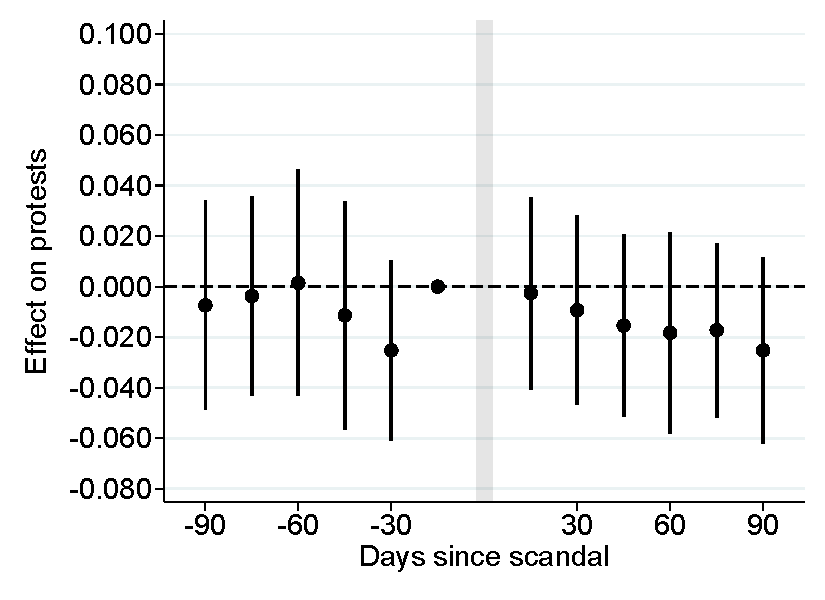
\includegraphics[width=\textwidth]{es_num_peaceful_MM_w90_b15_na_ols_90ci.pdf}\end{subfigure}
    \end{center}
    \footnotesize{OLS event study estimated separately on the Apex and Non-Apex subsamples, on 15-day event-time bin indicators over the $\pm 90$-day window. The four panels are violent and peaceful protests $\times$ Apex and Non-Apex; the reference bin (the 15 days before disclosure) is normalized to zero and shown at its position, and the faint thick vertical line marks the disclosure cutoff. All four panels share a common y-axis. Vertical bars are 90\% confidence intervals; standard errors clustered at country $\times$ year $\times$ day-bin. Sample period 2008--2019; Venezuela excluded.}
\end{figure}

\begin{comment}
\begin{figure}[htb!]
    \caption{Event studies, $\pm 120$-day window (15-day bins).}
    \label{fig:sup_es_w120}
    \begin{center}
    \begin{subfigure}{0.45\textwidth}\caption{Violent, Apex.}
        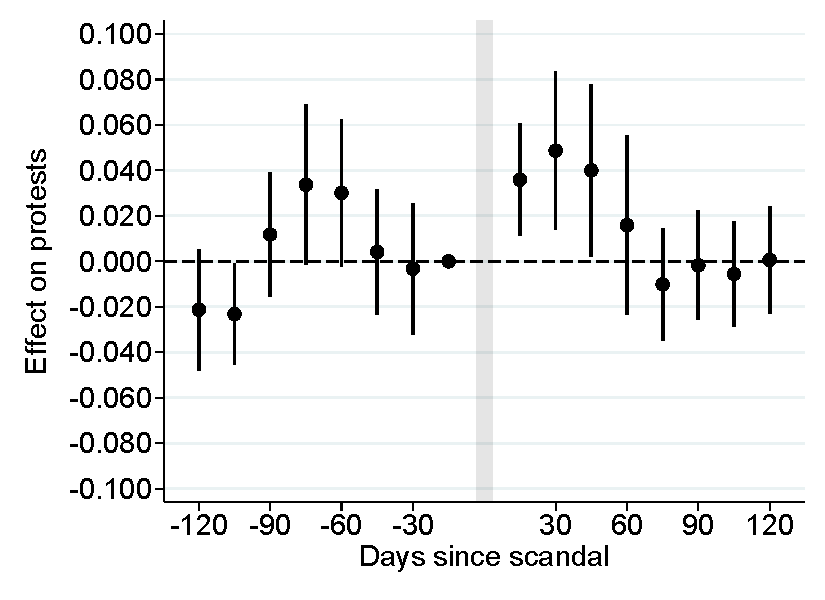
\includegraphics[width=\textwidth]{es_num_violent_MM_w120_b15_pa_ols_90ci.pdf}\end{subfigure}\hfill
    \begin{subfigure}{0.45\textwidth}\caption{Peaceful, Apex.}
        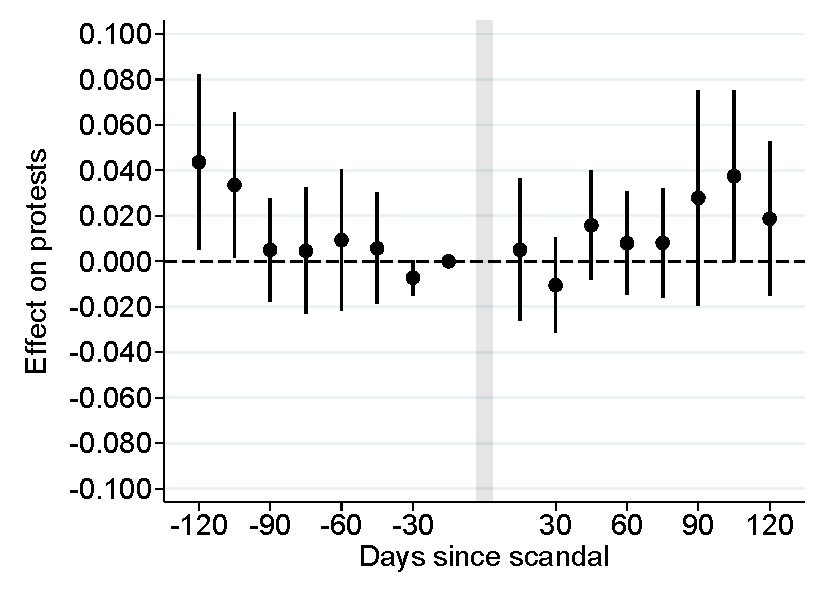
\includegraphics[width=\textwidth]{es_num_peaceful_MM_w120_b15_pa_ols_90ci.pdf}\end{subfigure} \\
    \begin{subfigure}{0.45\textwidth}\caption{Violent, Non-Apex.}
        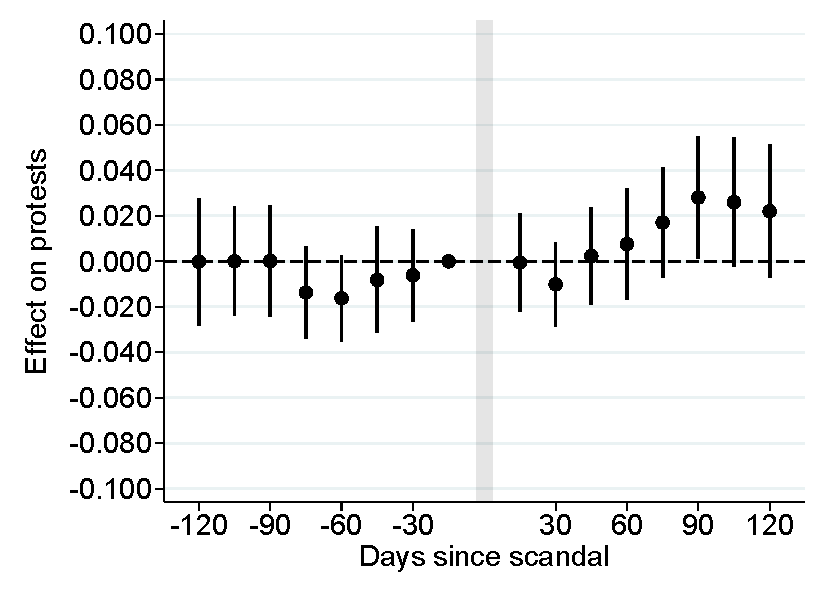
\includegraphics[width=\textwidth]{es_num_violent_MM_w120_b15_na_ols_90ci.pdf}\end{subfigure}\hfill
    \begin{subfigure}{0.45\textwidth}\caption{Peaceful, Non-Apex.}
        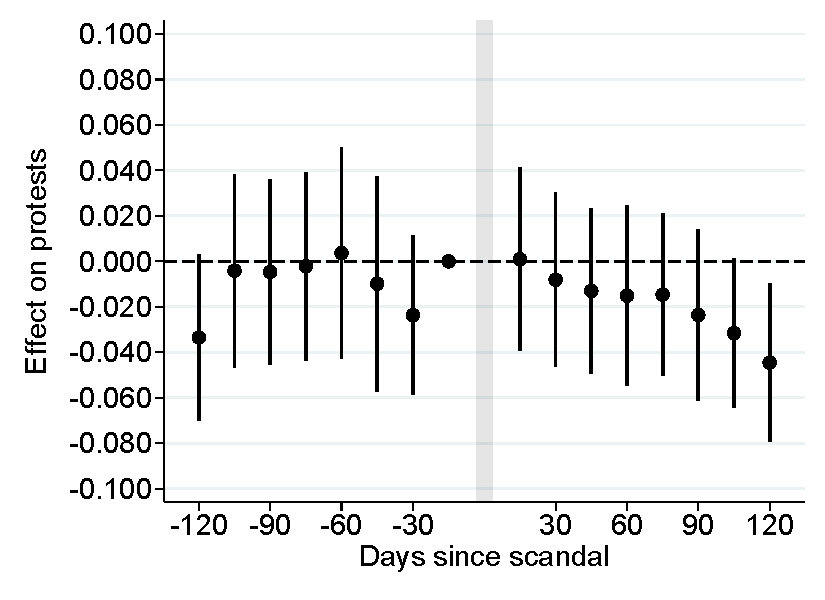
\includegraphics[width=\textwidth]{es_num_peaceful_MM_w120_b15_na_ols_90ci.pdf}\end{subfigure}
    \end{center}
    \footnotesize{OLS event study estimated separately on the Apex and Non-Apex subsamples, on 15-day event-time bin indicators over the $\pm 120$-day window. The four panels are violent and peaceful protests $\times$ Apex and Non-Apex; the reference bin (the 15 days before disclosure) is normalized to zero and shown at its position, and the faint thick vertical line marks the disclosure cutoff. All four panels share a common y-axis. Vertical bars are 90\% confidence intervals; standard errors clustered at country $\times$ year $\times$ day-bin. Sample period 2008--2019; Venezuela excluded.}
\end{figure}

% ---------------------------------------------------------------------
\clearpage
\section{Event studies with 30-day bins}\label{sup:es_b30}

Figures~\ref{fig:sup_es_b30_w60}--\ref{fig:sup_es_b30_w120} reproduce the event studies using 30-day bins instead of the 15-day bins used in the main text, for $T \in \{60, 90, 120\}$ (the $\pm 30$-day window admits only one bin per side at this width and is therefore omitted). As above, the four panels within each figure share a common y-axis.

\begin{figure}[htb!]
    \caption{Event studies, $\pm 60$-day window (30-day bins).}
    \label{fig:sup_es_b30_w60}
    \begin{center}
    \begin{subfigure}{0.45\textwidth}\caption{Violent, Apex.}
        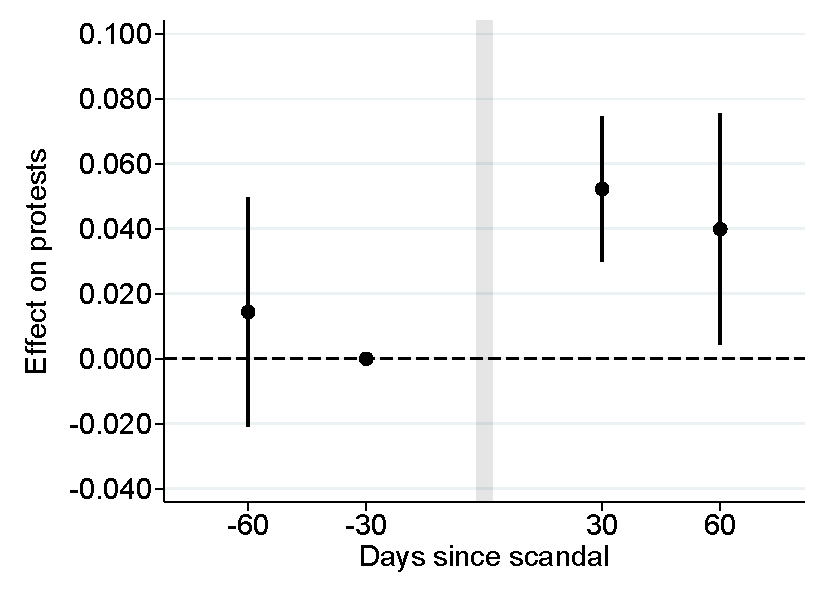
\includegraphics[width=\textwidth]{es_num_violent_MM_w60_b30_pa_ols_90ci.pdf}\end{subfigure}\hfill
    \begin{subfigure}{0.45\textwidth}\caption{Peaceful, Apex.}
        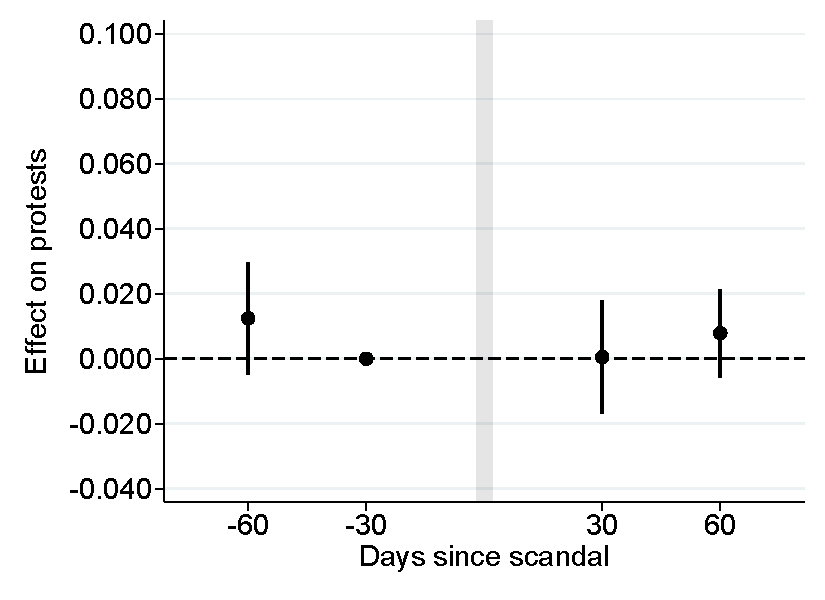
\includegraphics[width=\textwidth]{es_num_peaceful_MM_w60_b30_pa_ols_90ci.pdf}\end{subfigure} \\
    \begin{subfigure}{0.45\textwidth}\caption{Violent, Non-Apex.}
        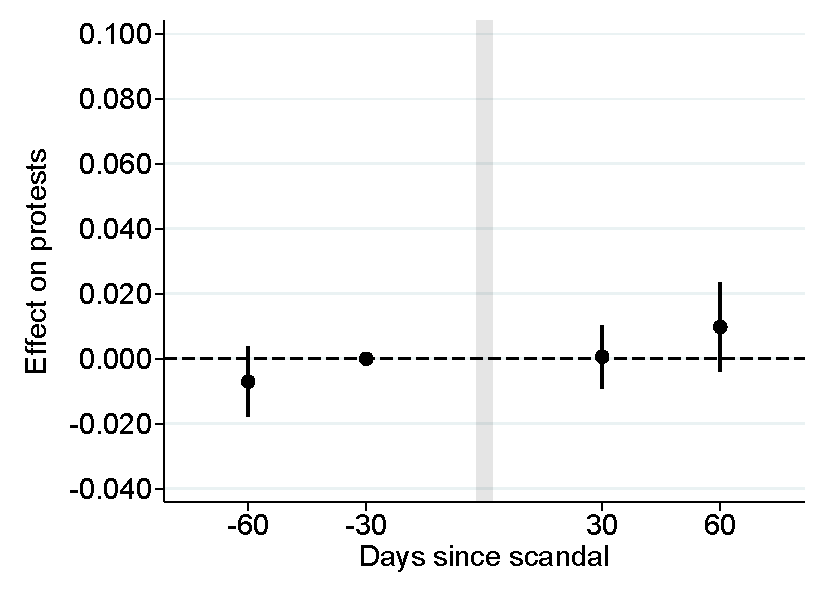
\includegraphics[width=\textwidth]{es_num_violent_MM_w60_b30_na_ols_90ci.pdf}\end{subfigure}\hfill
    \begin{subfigure}{0.45\textwidth}\caption{Peaceful, Non-Apex.}
        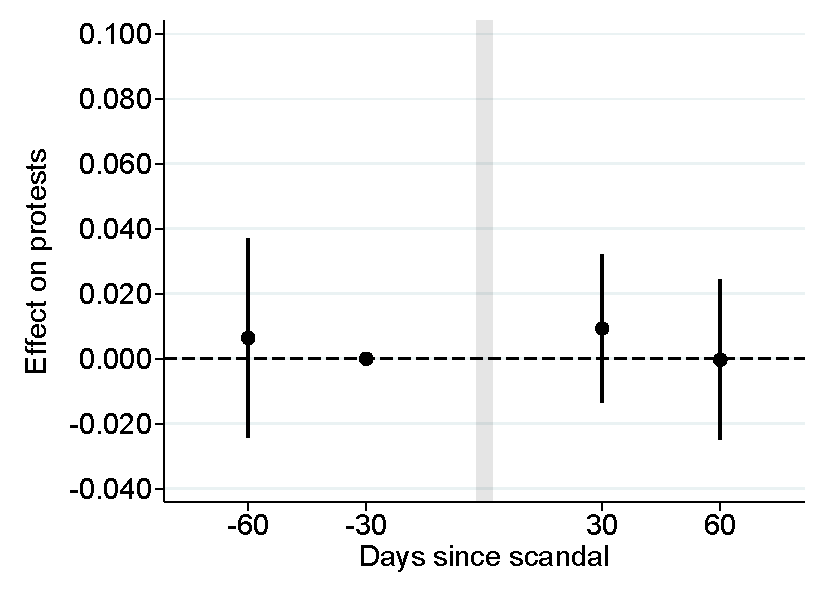
\includegraphics[width=\textwidth]{es_num_peaceful_MM_w60_b30_na_ols_90ci.pdf}\end{subfigure}
    \end{center}
    \footnotesize{OLS event study estimated separately on the Apex and Non-Apex subsamples, on 30-day event-time bin indicators over the $\pm 60$-day window (the 30-day-bin analog of the main-text event studies). The four panels are violent and peaceful protests $\times$ Apex and Non-Apex; the reference bin (the 30 days before disclosure) is normalized to zero and shown at its position, and the faint thick vertical line marks the disclosure cutoff. All four panels share a common y-axis. Vertical bars are 90\% confidence intervals; standard errors clustered at country $\times$ year $\times$ day-bin. Sample period 2008--2019; Venezuela excluded.}
\end{figure}

\begin{figure}[htb!]
    \caption{Event studies, $\pm 90$-day window (30-day bins).}
    \label{fig:sup_es_b30_w90}
    \begin{center}
    \begin{subfigure}{0.45\textwidth}\caption{Violent, Apex.}
        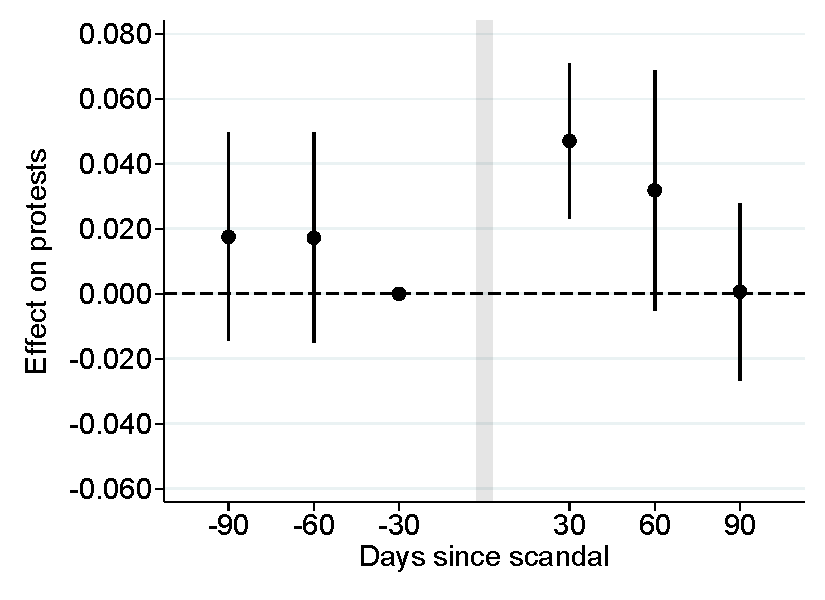
\includegraphics[width=\textwidth]{es_num_violent_MM_w90_b30_pa_ols_90ci.pdf}\end{subfigure}\hfill
    \begin{subfigure}{0.45\textwidth}\caption{Peaceful, Apex.}
        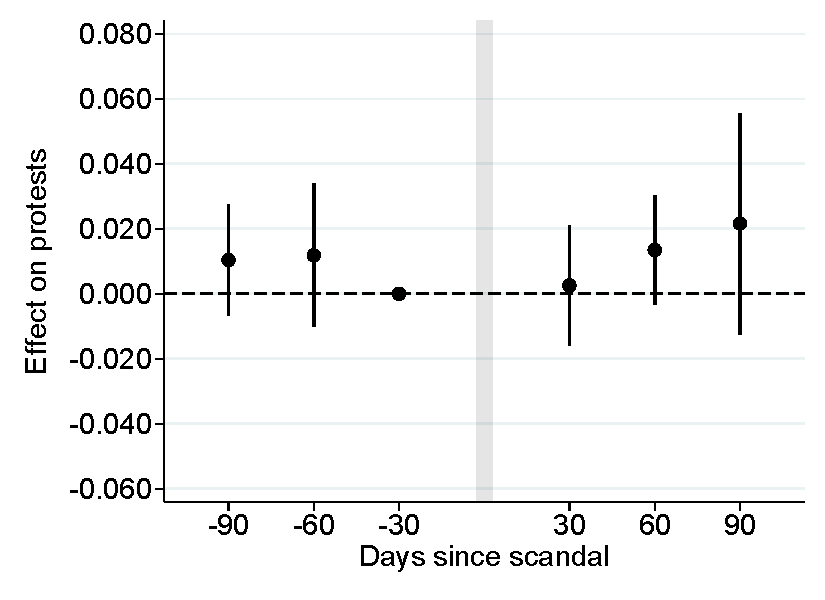
\includegraphics[width=\textwidth]{es_num_peaceful_MM_w90_b30_pa_ols_90ci.pdf}\end{subfigure} \\
    \begin{subfigure}{0.45\textwidth}\caption{Violent, Non-Apex.}
        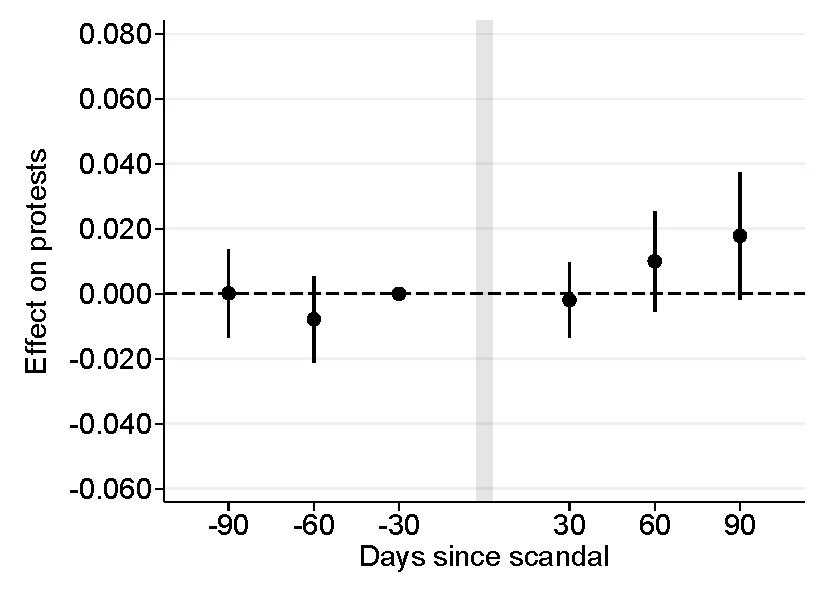
\includegraphics[width=\textwidth]{es_num_violent_MM_w90_b30_na_ols_90ci.pdf}\end{subfigure}\hfill
    \begin{subfigure}{0.45\textwidth}\caption{Peaceful, Non-Apex.}
        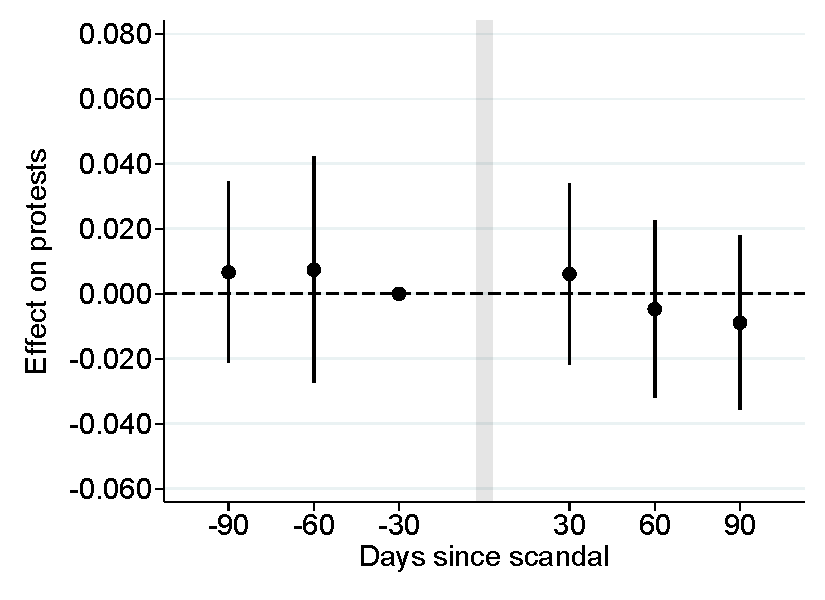
\includegraphics[width=\textwidth]{es_num_peaceful_MM_w90_b30_na_ols_90ci.pdf}\end{subfigure}
    \end{center}
    \footnotesize{OLS event study estimated separately on the Apex and Non-Apex subsamples, on 30-day event-time bin indicators over the $\pm 90$-day window. The four panels are violent and peaceful protests $\times$ Apex and Non-Apex; the reference bin (the 30 days before disclosure) is normalized to zero and shown at its position, and the faint thick vertical line marks the disclosure cutoff. All four panels share a common y-axis. Vertical bars are 90\% confidence intervals; standard errors clustered at country $\times$ year $\times$ day-bin. Sample period 2008--2019; Venezuela excluded.}
\end{figure}

\begin{figure}[htb!]
    \caption{Event studies, $\pm 120$-day window (30-day bins).}
    \label{fig:sup_es_b30_w120}
    \begin{center}
    \begin{subfigure}{0.45\textwidth}\caption{Violent, Apex.}
        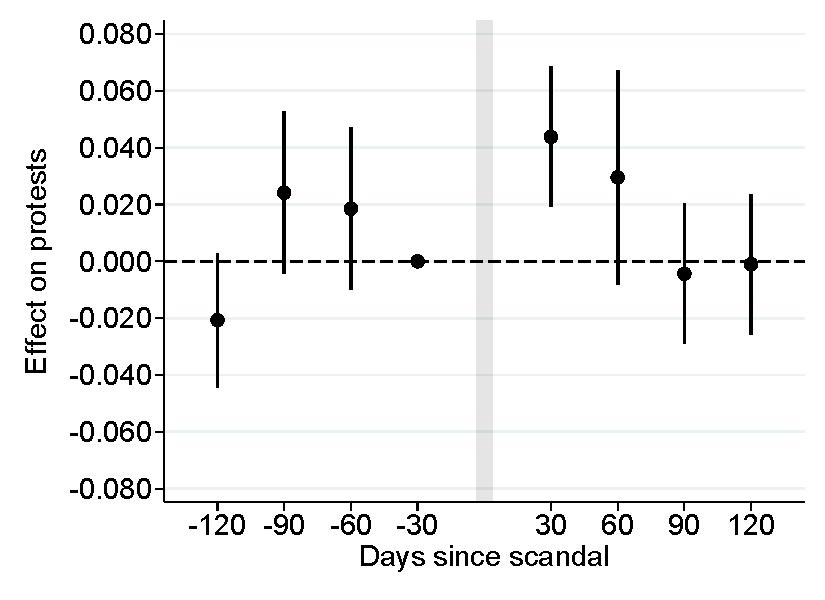
\includegraphics[width=\textwidth]{es_num_violent_MM_w120_b30_pa_ols_90ci.pdf}\end{subfigure}\hfill
    \begin{subfigure}{0.45\textwidth}\caption{Peaceful, Apex.}
        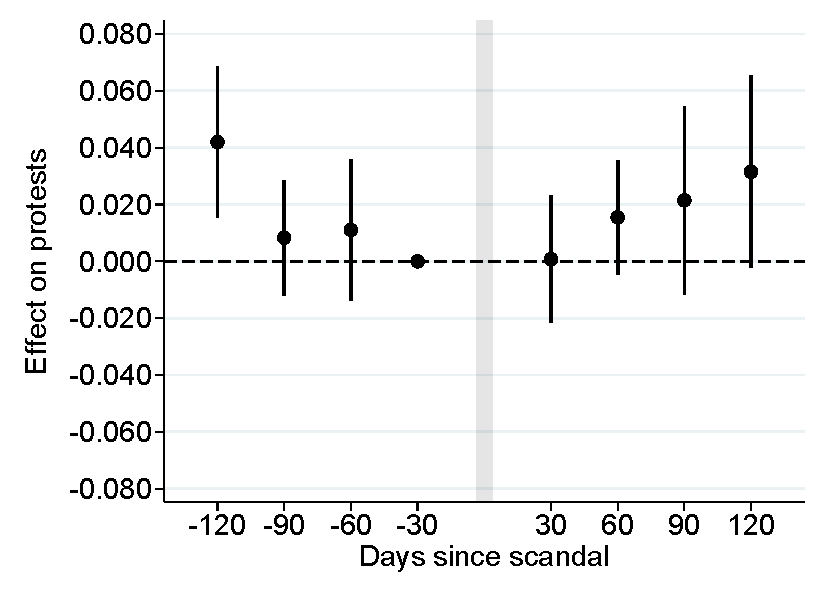
\includegraphics[width=\textwidth]{es_num_peaceful_MM_w120_b30_pa_ols_90ci.pdf}\end{subfigure} \\
    \begin{subfigure}{0.45\textwidth}\caption{Violent, Non-Apex.}
        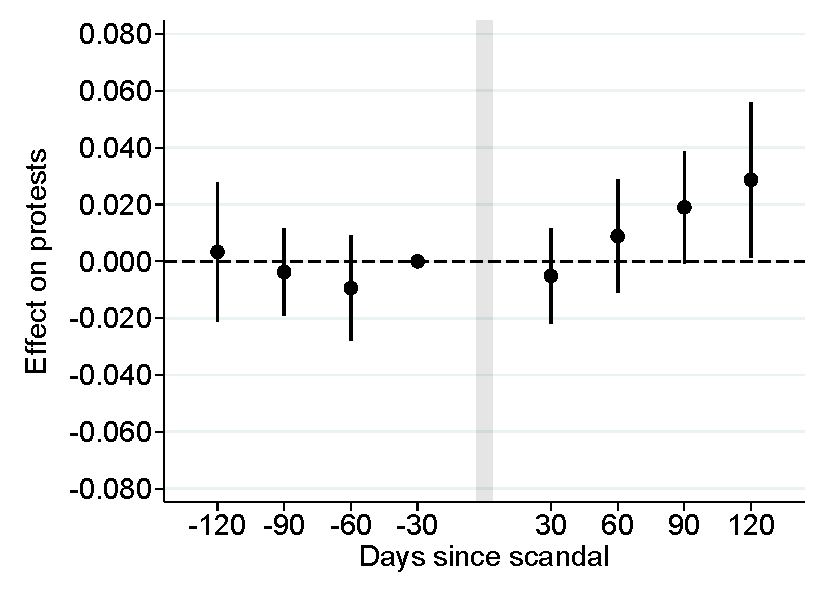
\includegraphics[width=\textwidth]{es_num_violent_MM_w120_b30_na_ols_90ci.pdf}\end{subfigure}\hfill
    \begin{subfigure}{0.45\textwidth}\caption{Peaceful, Non-Apex.}
        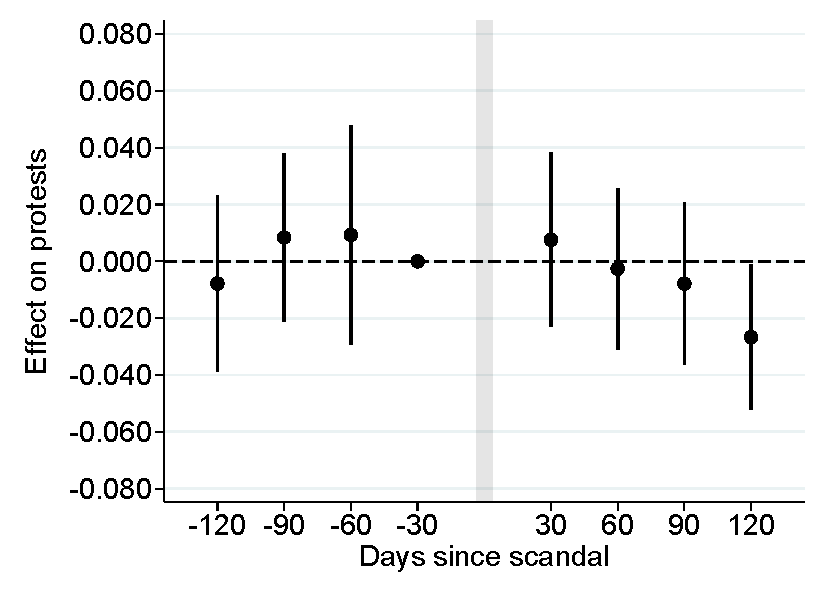
\includegraphics[width=\textwidth]{es_num_peaceful_MM_w120_b30_na_ols_90ci.pdf}\end{subfigure}
    \end{center}
    \footnotesize{OLS event study estimated separately on the Apex and Non-Apex subsamples, on 30-day event-time bin indicators over the $\pm 120$-day window---the 30-day-bin counterpart to the main-text \autoref{fig:dynamics}. The four panels are violent and peaceful protests $\times$ Apex and Non-Apex; the reference bin (the 30 days before disclosure) is normalized to zero and shown at its position, and the faint thick vertical line marks the disclosure cutoff. All four panels share a common y-axis. Vertical bars are 90\% confidence intervals; standard errors clustered at country $\times$ year $\times$ day-bin. Sample period 2008--2019; Venezuela excluded.}
\end{figure}
\end{comment}

% ---------------------------------------------------------------------
\clearpage

% ---------------------------------------------------------------------
\clearpage
\begin{comment}
\section{Restricted subsamples: Presidential and Apex}\label{sup:restricted}

Tables~\ref{tab:sup_pres_only} and \ref{tab:sup_pres_apex} re-estimate \autoref{eq:main} on progressively narrower subsamples: scandals implicating a sitting President only (45 scandals), and Presidents plus Other Apex officials (63 scandals). Each table reports OLS estimates of \autoref{eq:main} on the eight outcomes. The violent-protest effect is present in the President-only sample and remains when Other Apex scandals are added.

\begin{table}[htb!]
    \caption{Table~\ref{tab:main} restricted to Presidential scandals.}
    \label{tab:sup_pres_only}
    \begin{center}
        \scriptsize{{
\def\sym#1{\ifmmode^{#1}\else\(^{#1}\)\fi}
\begin{tabular}{l*{8}{c}}
\toprule
&\multicolumn{2}{c}{$\pm 30$-Day Window}    &\multicolumn{2}{c}{$\pm 120$-Day Window}   &\multicolumn{2}{c}{Shares ($\pm 30$-Day)}  &\multicolumn{2}{c}{Shares ($\pm 120$-Day)} \\\cmidrule(lr){2-3}\cmidrule(lr){4-5}\cmidrule(lr){6-7}\cmidrule(lr){8-9}
&\multicolumn{1}{c}{(1)}&\multicolumn{1}{c}{(2)}&\multicolumn{1}{c}{(3)}&\multicolumn{1}{c}{(4)}&\multicolumn{1}{c}{(5)}&\multicolumn{1}{c}{(6)}&\multicolumn{1}{c}{(7)}&\multicolumn{1}{c}{(8)}\\
&\multicolumn{1}{c}{\shortstack{Violent\\Protests}}&\multicolumn{1}{c}{\shortstack{Peaceful\\Protests}}&\multicolumn{1}{c}{\shortstack{Violent\\Protests}}&\multicolumn{1}{c}{\shortstack{Peaceful\\Protests}}&\multicolumn{1}{c}{\shortstack{Share\\Violent}}&\multicolumn{1}{c}{\shortstack{Share\\Peaceful}}&\multicolumn{1}{c}{\shortstack{Share\\Violent}}&\multicolumn{1}{c}{\shortstack{Share\\Peaceful}}\\
\midrule \multicolumn{9}{l}{\textbf{\textit{Panel A: OLS}}} \\
Post Scandal&       0.035\sym{*}  &       0.006         &       0.007         &      -0.003         &       0.034\sym{*}  &       0.004         &       0.006         &      -0.005         \\
&     (0.018)         &     (0.005)         &     (0.008)         &     (0.010)         &     (0.018)         &     (0.004)         &     (0.008)         &     (0.009)         \\
\midrule
Mean (Pre-Scandal Bin)&       0.000         &       0.015         &       0.003         &       0.009         &       0.000         &       0.015         &       0.003         &       0.009         \\
Observations&        2745         &        2745         &       10845         &       10845         &        2745         &        2745         &       10845         &       10845         \\
Number of Scandals&          45         &          45         &          45         &          45         &          45         &          45         &          45         &          45         \\
R-squared   &       0.098         &       0.036         &       0.114         &       0.164         &       0.099         &       0.034         &       0.118         &       0.159         \\
\midrule
\multicolumn{9}{l}{\textbf{\textit{Panel B: Poisson QML}}} \\
Post Scandal (IRR)&      66.637\sym{*}  &       1.350         &       0.979         &       0.666          & & & & \\
&   (146.660)         &     (0.576)         &     (0.420)         &     (0.211)          & & & & \\
\midrule
Mean (Pre-Scandal Bin)&       0.000         &       0.056         &       0.008         &       0.011          & & & & \\
Observations&         532         &         796         &        3386         &        8216          & & & & \\
Number of Scandals&          14         &          19         &          22         &          35          & & & & \\
Pseudo R-squared&       0.301         &       0.118         &       0.267         &       0.290          & & & & \\
\bottomrule
\end{tabular}
}
}
    \end{center}
    \footnotesize{OLS estimates of $\beta$ from \autoref{eq:main} on the eight outcomes (cols.\ 1--4 counts, cols.\ 5--8 shares). Subsample: the 45 scandals classified as ``President'' in \autoref{sup:classification}. Standard errors (in parentheses) clustered at the country $\times$ year $\times$ day-bin level. Same fixed effects, sample period, and clustering as Table~\ref{tab:main}.}
\end{table}

\begin{table}[htb!]
    \caption{Table~\ref{tab:main} restricted to President and Other Apex scandals.}
    \label{tab:sup_pres_apex}
    \begin{center}
        \scriptsize{{
\def\sym#1{\ifmmode^{#1}\else\(^{#1}\)\fi}
\begin{tabular}{l*{8}{c}}
\toprule
&\multicolumn{2}{c}{$\pm 30$-Day Window}    &\multicolumn{2}{c}{$\pm 120$-Day Window}   &\multicolumn{2}{c}{Shares ($\pm 30$-Day)}  &\multicolumn{2}{c}{Shares ($\pm 120$-Day)} \\\cmidrule(lr){2-3}\cmidrule(lr){4-5}\cmidrule(lr){6-7}\cmidrule(lr){8-9}
&\multicolumn{1}{c}{(1)}&\multicolumn{1}{c}{(2)}&\multicolumn{1}{c}{(3)}&\multicolumn{1}{c}{(4)}&\multicolumn{1}{c}{(5)}&\multicolumn{1}{c}{(6)}&\multicolumn{1}{c}{(7)}&\multicolumn{1}{c}{(8)}\\
&\multicolumn{1}{c}{\shortstack{Violent\\Protests}}&\multicolumn{1}{c}{\shortstack{Peaceful\\Protests}}&\multicolumn{1}{c}{\shortstack{Violent\\Protests}}&\multicolumn{1}{c}{\shortstack{Peaceful\\Protests}}&\multicolumn{1}{c}{\shortstack{Share\\Violent}}&\multicolumn{1}{c}{\shortstack{Share\\Peaceful}}&\multicolumn{1}{c}{\shortstack{Share\\Violent}}&\multicolumn{1}{c}{\shortstack{Share\\Peaceful}}\\
\midrule \multicolumn{9}{l}{\textbf{\textit{Panel A: OLS}}} \\
Post Scandal&       0.060\sym{***}&       0.005         &       0.021\sym{*}  &       0.002         &       0.060\sym{***}&       0.005         &       0.021\sym{*}  &      -0.000         \\
&     (0.017)         &     (0.008)         &     (0.012)         &     (0.010)         &     (0.017)         &     (0.008)         &     (0.012)         &     (0.009)         \\
\midrule
Mean (Pre-Scandal Bin)&       0.036         &       0.018         &       0.027         &       0.015         &       0.036         &       0.018         &       0.027         &       0.014         \\
Observations&        3904         &        3904         &       15665         &       15665         &        3904         &        3904         &       15665         &       15665         \\
Number of Scandals&          64         &          64         &          64         &          64         &          64         &          64         &          64         &          64         \\
R-squared   &       0.270         &       0.075         &       0.193         &       0.117         &       0.275         &       0.081         &       0.197         &       0.116         \\
\midrule
\multicolumn{9}{l}{\textbf{\textit{Panel B: Poisson QML}}} \\
Post Scandal (IRR)&       2.180\sym{**} &       1.138         &       1.375\sym{*}  &       1.083          & & & & \\
&     (0.660)         &     (0.556)         &     (0.253)         &     (0.303)          & & & & \\
\midrule
Mean (Pre-Scandal Bin)&       0.101         &       0.041         &       0.054         &       0.018          & & & & \\
Observations&        1397         &        1778         &        7519         &       12613          & & & & \\
Number of Scandals&          28         &          32         &          34         &          53          & & & & \\
Pseudo R-squared&       0.299         &       0.170         &       0.339         &       0.220          & & & & \\
\bottomrule
\end{tabular}
}
}
    \end{center}
    \footnotesize{As in Table~\ref{tab:sup_pres_only}, restricted to the 63 scandals classified as ``President'' or ``Other Apex'' in \autoref{sup:classification}.}
\end{table}
\end{comment}

% ---------------------------------------------------------------------
\clearpage
% Regression-based hierarchy analysis removed per author request.
\begin{comment}
\section{Regression-based hierarchy analysis}\label{sup:hierarchy}

Table~\ref{tab:sup_hierarchy} reports the pooled-regression analogue of the apex partition, splitting the interaction into all three bins. For each outcome and window we estimate
\begin{equation*}
    Y_{c(s)t} \;=\; \beta_{\text{Pres}}\, \mathrm{Post}_{st}\, \mathbf{1}\{\text{Pres}_s\}
    \;+\; \beta_{\text{OA}}\, \mathrm{Post}_{st}\, \mathbf{1}\{\text{OA}_s\}
    \;+\; \beta_{\text{ONA}}\, \mathrm{Post}_{st}\, \mathbf{1}\{\text{ONA}_s\}
    \;+\; \alpha_d + \lambda_m + \theta_{cy} + \varepsilon_{c(s)t},
\end{equation*}
where $\mathrm{Pres}_s$, $\mathrm{OA}_s$, $\mathrm{ONA}_s$ are scandal-level indicators for President, Other Apex, and Non-Apex. The specification omits a stand-alone Post term, so each coefficient is the average post-scandal effect for that category, and we report the $p$-values from pairwise equality tests.

\begin{table}[htb!]
    \caption{Pooled interaction regression: hierarchy of the protest response.}
    \label{tab:sup_hierarchy}
    \begin{center}
        \scriptsize{{
\def\sym#1{\ifmmode^{#1}\else\(^{#1}\)\fi}
\begin{tabular}{l*{4}{c}}
\toprule
            &\multicolumn{2}{c}{$\pm 30$-Day Window}    &\multicolumn{2}{c}{Shares ($\pm 30$-Day)}  \\\cmidrule(lr){2-3}\cmidrule(lr){4-5}
            &\multicolumn{1}{c}{(1)}&\multicolumn{1}{c}{(2)}&\multicolumn{1}{c}{(3)}&\multicolumn{1}{c}{(4)}\\
            &\multicolumn{1}{c}{\shortstack{Violent\\Protests}}&\multicolumn{1}{c}{\shortstack{Peaceful\\Protests}}&\multicolumn{1}{c}{\shortstack{Share\\Violent}}&\multicolumn{1}{c}{\shortstack{Share\\Peaceful}}\\
\midrule
Post $\times$ President&       0.028\sym{***}&      -0.001         &       0.027\sym{***}&      -0.001         \\
            &     (0.009)         &     (0.009)         &     (0.009)         &     (0.008)         \\
Post $\times$ Other Apex&       0.112\sym{**} &      -0.021         &       0.113\sym{**} &      -0.015         \\
            &     (0.047)         &     (0.031)         &     (0.047)         &     (0.028)         \\
Post $\times$ Other Non-Apex&      -0.004         &       0.019         &      -0.005         &       0.019         \\
            &     (0.007)         &     (0.013)         &     (0.007)         &     (0.013)         \\
\midrule
p-value: President $$=$$ Other Non-Apex&       0.006         &       0.237         &       0.005         &       0.215         \\
p-value: Other Apex $$=$$ Other Non-Apex&       0.028         &       0.303         &       0.025         &       0.336         \\
p-value: President $$=$$ Other Apex&       0.066         &       0.478         &       0.058         &       0.570         \\
Mean (Pre-Scandal Bin)&       0.027         &       0.069         &       0.027         &       0.061         \\
Observations&       10736         &       10736         &       10736         &       10736         \\
Number of Scandals&         176         &         176         &         176         &         176         \\
R-squared   &       0.178         &       0.474         &       0.186         &       0.494         \\
\bottomrule
\end{tabular}
}
}
    \end{center}
    \footnotesize{OLS estimates of $\beta_{\text{Pres}}$, $\beta_{\text{OA}}$, $\beta_{\text{ONA}}$ (Post $\times$ President, Other Apex, Non-Apex) on the four count outcomes (cols.\ 1--4) and four share outcomes (cols.\ 5--8). Standard errors (in parentheses) clustered at the country $\times$ year $\times$ day-bin level. Fixed effects, sample period, and clustering identical to Table~\ref{tab:main}. Rows labeled ``$p$-value'' report pairwise equality tests across the three category coefficients.}
\end{table}
\end{comment}

% ---------------------------------------------------------------------
\clearpage
% Electoral-democracy split moved to the main body (Low vs. Medium+High table).
% Liberal-index and Freedom House versions are kept below as robustness.
\begin{comment}
\section{Heterogeneity by democracy: tercile split}\label{sup:democracy_terciles}

Table~\ref{tab:democracy} in the main text splits countries at the \emph{median} of their 2008 democracy score. \autoref{tab:sup_democracy_terciles} refines that split into \emph{terciles} of V-Dem's 2008 Electoral Democracy Index: Low (bottom tercile), Medium (middle tercile), and High (top tercile). Alongside the three interaction coefficients, it reports the one-sided $p$-values for the orderings $\beta_{\text{High}}>\beta_{\text{Medium}}$, $\beta_{\text{Medium}}>\beta_{\text{Low}}$, and $\beta_{\text{High}}>\beta_{\text{Low}}$. The violent-protest effect is, if anything, increasing in democracy: at the $\pm 90$- and $\pm 120$-day windows the High-democracy effect exceeds the Low-democracy effect at conventional one-sided significance ($p=0.040$ and $0.042$).

\begin{table}[htb!]
    \caption{Effect by 2008 level of democracy, tercile split.}
    \label{tab:sup_democracy_terciles}
    \begin{center}
        \scriptsize{{
\def\sym#1{\ifmmode^{#1}\else\(^{#1}\)\fi}
\begin{tabular}{l*{8}{c}}
\toprule
            &\multicolumn{2}{c}{$\pm 30$-Day Window}    &\multicolumn{2}{c}{$\pm 60$-Day Window}    &\multicolumn{2}{c}{$\pm 90$-Day Window}    &\multicolumn{2}{c}{$\pm 120$-Day Window}   \\\cmidrule(lr){2-3}\cmidrule(lr){4-5}\cmidrule(lr){6-7}\cmidrule(lr){8-9}
            &\multicolumn{1}{c}{(1)}&\multicolumn{1}{c}{(2)}&\multicolumn{1}{c}{(3)}&\multicolumn{1}{c}{(4)}&\multicolumn{1}{c}{(5)}&\multicolumn{1}{c}{(6)}&\multicolumn{1}{c}{(7)}&\multicolumn{1}{c}{(8)}\\
            &\multicolumn{1}{c}{\shortstack{Violent\\Protests}}&\multicolumn{1}{c}{\shortstack{Peaceful\\Protests}}&\multicolumn{1}{c}{\shortstack{Violent\\Protests}}&\multicolumn{1}{c}{\shortstack{Peaceful\\Protests}}&\multicolumn{1}{c}{\shortstack{Violent\\Protests}}&\multicolumn{1}{c}{\shortstack{Peaceful\\Protests}}&\multicolumn{1}{c}{\shortstack{Violent\\Protests}}&\multicolumn{1}{c}{\shortstack{Peaceful\\Protests}}\\
\midrule
Post $\times$ High Democracy (2008)&       0.006         &       0.011         &       0.019\sym{***}&       0.005         &       0.012         &      -0.006         &       0.014\sym{*}  &      -0.012         \\
            &     (0.005)         &     (0.010)         &     (0.007)         &     (0.014)         &     (0.007)         &     (0.012)         &     (0.007)         &     (0.011)         \\
Post $\times$ Medium Democracy (2008)&       0.028\sym{*}  &       0.015         &       0.023         &      -0.006         &       0.022         &      -0.005         &       0.027         &      -0.009         \\
            &     (0.015)         &     (0.010)         &     (0.018)         &     (0.009)         &     (0.018)         &     (0.008)         &     (0.019)         &     (0.009)         \\
Post $\times$ Low Democracy (2008)&       0.012\sym{**} &       0.005         &       0.010\sym{*}  &       0.003         &       0.002         &       0.001         &       0.005         &      -0.005         \\
            &     (0.006)         &     (0.014)         &     (0.006)         &     (0.018)         &     (0.005)         &     (0.015)         &     (0.004)         &     (0.014)         \\
\midrule
p-value: High $>$ Medium (one-sided)&       0.916         &       0.620         &       0.574         &       0.260         &       0.699         &       0.528         &       0.748         &       0.572         \\
p-value: Medium $>$ Low (one-sided)&       0.176         &       0.252         &       0.267         &       0.665         &       0.143         &       0.631         &       0.121         &       0.600         \\
p-value: High $>$ Low (one-sided)&       0.859         &       0.343         &       0.148         &       0.460         &       0.112         &       0.644         &       0.109         &       0.651         \\
Mean (Pre-Scandal)&       0.020         &       0.053         &       0.021         &       0.056         &       0.024         &       0.057         &       0.023         &       0.058         \\
Observations&       10614         &       10614         &       21054         &       21054         &       31494         &       31494         &       41934         &       41934         \\
Number of Scandals&         174         &         174         &         174         &         174         &         174         &         174         &         174         &         174         \\
R-squared   &       0.165         &       0.478         &       0.158         &       0.398         &       0.136         &       0.349         &       0.131         &       0.301         \\
\bottomrule
\end{tabular}
}
}
    \end{center}
    \footnotesize{OLS estimates of $\beta_{\text{High}}$, $\beta_{\text{Medium}}$, and $\beta_{\text{Low}}$, the coefficients on the post-scandal indicator interacted with top-, middle-, and bottom-tercile 2008-democracy flags. Columns are violent and peaceful protest counts at four event-window widths: $\pm$30 days (cols.\ 1--2), $\pm$60 (cols.\ 3--4), $\pm$90 (cols.\ 5--6), and $\pm$120 (cols.\ 7--8). The 16 sample countries are grouped into terciles of V-Dem's Electoral Democracy Index (\texttt{v2x\_polyarchy}) in 2008. An observation is a country-day inside a scandal's event window. The rows ``$p$-value: High $>$ Medium,'' ``Medium $>$ Low,'' and ``High $>$ Low'' report the one-sided $p$-values for the corresponding orderings of the coefficients. All specifications include country-by-year, month-of-year, and day-of-week fixed effects; standard errors (in parentheses) are clustered at the country $\times$ year $\times$ day-bin level. Sample period 2008--2019; Venezuela excluded. Significance: $^{*}$ $p<0.1$, $^{**}$ $p<0.05$, $^{***}$ $p<0.01$.}
\end{table}

Pooling the top two terciles into a single ``Medium+High'' group sharpens the comparison against the bottom tercile. \autoref{tab:sup_democracy_lmh} reports this Low vs.\ Medium+High split. The violent-protest effect is larger in the Medium+High group at every window, and the one-sided ordering $\beta_{\text{Medium+High}}>\beta_{\text{Low}}$ is significant at the $\pm 90$- and $\pm 120$-day windows ($p=0.037$ and $0.033$).

\begin{table}[htb!]
    \caption{Effect by 2008 level of democracy: Low vs.\ Medium+High.}
    \label{tab:sup_democracy_lmh}
    \begin{center}
        \scriptsize{{
\def\sym#1{\ifmmode^{#1}\else\(^{#1}\)\fi}
\begin{tabular}{l*{6}{c}}
\toprule
            &\multicolumn{2}{c}{$\pm 30$-Day Window}    &\multicolumn{2}{c}{$\pm 60$-Day Window}    &\multicolumn{2}{c}{$\pm 90$-Day Window}    \\\cmidrule(lr){2-3}\cmidrule(lr){4-5}\cmidrule(lr){6-7}
            &\multicolumn{1}{c}{(1)}&\multicolumn{1}{c}{(2)}&\multicolumn{1}{c}{(3)}&\multicolumn{1}{c}{(4)}&\multicolumn{1}{c}{(5)}&\multicolumn{1}{c}{(6)}\\
            &\multicolumn{1}{c}{\shortstack{Violent\\Protests}}&\multicolumn{1}{c}{\shortstack{Peaceful\\Protests}}&\multicolumn{1}{c}{\shortstack{Violent\\Protests}}&\multicolumn{1}{c}{\shortstack{Peaceful\\Protests}}&\multicolumn{1}{c}{\shortstack{Violent\\Protests}}&\multicolumn{1}{c}{\shortstack{Peaceful\\Protests}}\\
\midrule
Post $\times$ Medium+High Democracy (2008)&       0.018\sym{**} &       0.012         &       0.021\sym{**} &       0.000         &       0.019\sym{**} &      -0.005         \\
            &     (0.007)         &     (0.008)         &     (0.008)         &     (0.008)         &     (0.009)         &     (0.007)         \\
Post $\times$ Low Democracy (2008)&       0.012\sym{**} &       0.005         &       0.010\sym{*}  &       0.003         &       0.001         &       0.001         \\
            &     (0.006)         &     (0.014)         &     (0.006)         &     (0.018)         &     (0.005)         &     (0.015)         \\
\midrule
p-value: Medium+High $=$ Low&       0.547         &       0.586         &       0.295         &       0.898         &       0.074         &       0.719         \\
p-value: Medium+High $>$ Low (one-sided)&       0.273         &       0.293         &       0.147         &       0.551         &       0.037         &       0.641         \\
Mean (Pre-Scandal)&       0.020         &       0.053         &       0.021         &       0.056         &       0.024         &       0.057         \\
Observations&       10736         &       10736         &       21296         &       21296         &       31856         &       31856         \\
Number of Scandals&         176         &         176         &         176         &         176         &         176         &         176         \\
R-squared   &       0.160         &       0.473         &       0.154         &       0.396         &       0.133         &       0.348         \\
\bottomrule
\end{tabular}
}
}
    \end{center}
    \footnotesize{OLS estimates of $\beta_{\text{Medium+High}}$ and $\beta_{\text{Low}}$, the coefficients on the post-scandal indicator interacted with a top-two-tercile (``Medium+High'') and a bottom-tercile (``Low'') 2008-democracy flag. Columns are violent and peaceful protest counts at four event-window widths: $\pm$30 days (cols.\ 1--2), $\pm$60 (cols.\ 3--4), $\pm$90 (cols.\ 5--6), and $\pm$120 (cols.\ 7--8). The 16 sample countries are split into terciles of V-Dem's Electoral Democracy Index (\texttt{v2x\_polyarchy}) in 2008, and the top two terciles are pooled. An observation is a country-day inside a scandal's event window. ``$p$-value: Medium+High $=$ Low'' reports the two-sided $p$-value for $H_0:\beta_{\text{Medium+High}}=\beta_{\text{Low}}$; ``$p$-value: Medium+High $>$ Low (one-sided)'' reports the one-sided $p$-value for $H_1:\beta_{\text{Medium+High}}>\beta_{\text{Low}}$. All specifications include country-by-year, month-of-year, and day-of-week fixed effects; standard errors (in parentheses) are clustered at the country $\times$ year $\times$ day-bin level. Sample period 2008--2019; Venezuela excluded. Significance: $^{*}$ $p<0.1$, $^{**}$ $p<0.05$, $^{***}$ $p<0.01$.}
\end{table}
\end{comment}

% ---------------------------------------------------------------------
\clearpage
\section{Democracy: alternative indices and country classification}\label{sup:democracy_alt}

\autoref{tab:sup_democracy_index_ranks} lists the sample countries (sorted by their 2008 V-Dem Electoral Democracy Index, the index used in \autoref{tab:sup_democracy_lmh} in the main text) and shows how each is classified under four different 2008 democracy measures, so the tercile grouping is not an artefact of a single index. \autoref{tab:sup_democracy_terciles_libdem_lmh} then re-estimates the main-text Low vs.\ Medium+High split with V-Dem's Liberal Democracy Index, and \autoref{tab:sup_democracy_fh} with Freedom House's 2008 status (Free vs.\ Partly Free) in place of a continuous index. The ordering of the effects---larger where democracy is stronger---is preserved throughout.

\begin{table}[htb!]
    \caption{Country democracy classification across four indices.}
    \label{tab:sup_democracy_index_ranks}
    \begin{center}
        \small{\begin{tabular}{lcccc}
\toprule
 & V-Dem & V-Dem & & Freedom \\
Country & Electoral & Liberal & Polity2 & House \\
\midrule
Costa Rica & High & High & High & Free \\
Chile & High & High & High & Free \\
Brazil & High & High & Low & Free \\
Peru & High & High & High & Free \\
Argentina & High & High & Low & Free \\
Panama & Medium & Medium & High & Free \\
Paraguay & Low & Medium & Low & Partly Free \\
Colombia & Low & Medium & Low & Partly Free \\
Bolivia & Medium & Medium & Low & Partly Free \\
Mexico & Medium & Medium & Low & Free \\
Guatemala & Low & Low & Low & Partly Free \\
El Salvador & Low & Low & Low & Free \\
Ecuador & Medium & Low & Low & Partly Free \\
Dominican Republic & Medium & Low & Low & Free \\
Honduras & Low & Low & Low & Partly Free \\
Nicaragua & Low & Low & High & Partly Free \\
\bottomrule
\end{tabular}
}
    \end{center}
    \footnotesize{Each country's classification under four 2008 democracy measures. For the three continuous indices---V-Dem Electoral Democracy (\texttt{v2x\_polyarchy}), V-Dem Liberal Democracy (\texttt{v2x\_libdem}), and Polity2 (\texttt{e\_polity2})---the entry is the country's tercile (High / Medium / Low). Freedom House status (\texttt{e\_fh\_status}) is shown in its native categories (Free / Partly Free / Not Free). Polity2 discriminates poorly among these consolidated democracies (its scores cluster near the top), so its tercile split is noisier than the V-Dem indices. Countries are sorted by the V-Dem Electoral index.}
\end{table}

% Liberal-index robustness (the main-text split uses the Electoral index).  The
% 3-way tercile version is commented out; only the pooled Low-vs-Medium+High cut
% is shown, as the appendix table immediately after this comment block.
\begin{comment}
\begin{table}[htb!]
    \caption{Effect by 2008 level of democracy, tercile split: V-Dem Liberal Democracy Index.}
    \label{tab:sup_democracy_terciles_libdem}
    \begin{center}
        \scriptsize{{
\def\sym#1{\ifmmode^{#1}\else\(^{#1}\)\fi}
\begin{tabular}{l*{6}{c}}
\toprule
            &\multicolumn{2}{c}{$\pm 30$-Day Window}    &\multicolumn{2}{c}{$\pm 60$-Day Window}    &\multicolumn{2}{c}{$\pm 90$-Day Window}    \\\cmidrule(lr){2-3}\cmidrule(lr){4-5}\cmidrule(lr){6-7}
            &\multicolumn{1}{c}{(1)}&\multicolumn{1}{c}{(2)}&\multicolumn{1}{c}{(3)}&\multicolumn{1}{c}{(4)}&\multicolumn{1}{c}{(5)}&\multicolumn{1}{c}{(6)}\\
            &\multicolumn{1}{c}{\shortstack{Violent\\Protests}}&\multicolumn{1}{c}{\shortstack{Peaceful\\Protests}}&\multicolumn{1}{c}{\shortstack{Violent\\Protests}}&\multicolumn{1}{c}{\shortstack{Peaceful\\Protests}}&\multicolumn{1}{c}{\shortstack{Violent\\Protests}}&\multicolumn{1}{c}{\shortstack{Peaceful\\Protests}}\\
\midrule
Post $\times$ High Democracy (Liberal, 2008)&       0.006         &       0.011         &       0.019\sym{***}&       0.005         &       0.012         &      -0.006         \\
            &     (0.005)         &     (0.010)         &     (0.007)         &     (0.014)         &     (0.007)         &     (0.012)         \\
Post $\times$ Medium Democracy (Liberal, 2008)&       0.027\sym{**} &       0.023\sym{**} &       0.020         &       0.007         &       0.015         &       0.006         \\
            &     (0.012)         &     (0.010)         &     (0.014)         &     (0.011)         &     (0.012)         &     (0.011)         \\
Post $\times$ Low Democracy (Liberal, 2008)&       0.011\sym{*}  &      -0.006         &       0.011\sym{*}  &      -0.011         &       0.006         &      -0.009         \\
            &     (0.006)         &     (0.016)         &     (0.006)         &     (0.021)         &     (0.010)         &     (0.016)         \\
\midrule
p-value: High $>$ Medium (one-sided)&       0.946         &       0.823         &       0.531         &       0.555         &       0.598         &       0.763         \\
p-value: Medium $>$ Low (one-sided)&       0.111         &       0.062         &       0.271         &       0.227         &       0.266         &       0.230         \\
p-value: High $>$ Low (one-sided)&       0.787         &       0.178         &       0.176         &       0.268         &       0.304         &       0.424         \\
Mean (Pre-Scandal)&       0.020         &       0.053         &       0.021         &       0.056         &       0.024         &       0.057         \\
Observations&       10614         &       10614         &       21054         &       21054         &       31494         &       31494         \\
Number of Scandals&         174         &         174         &         174         &         174         &         174         &         174         \\
R-squared   &       0.165         &       0.478         &       0.158         &       0.398         &       0.136         &       0.349         \\
\bottomrule
\end{tabular}
}
}
    \end{center}
    \footnotesize{The electoral-index tercile split, but with terciles formed from V-Dem's 2008 \emph{Liberal} Democracy Index (\texttt{v2x\_libdem}) rather than the Electoral index. OLS estimates of $\beta_{\text{High}}$, $\beta_{\text{Medium}}$, and $\beta_{\text{Low}}$ (the post-scandal indicator interacted with top-, middle-, and bottom-tercile flags), on violent and peaceful protest counts at the $\pm$30/60/90-day windows. The rows report the one-sided $p$-values for the orderings High $>$ Medium, Medium $>$ Low, and High $>$ Low. All specifications include country-by-year, month-of-year, and day-of-week fixed effects; standard errors (in parentheses) are clustered at the country $\times$ year $\times$ day-bin level. Sample period 2008--2019; Venezuela excluded. Significance: $^{*}$ $p<0.1$, $^{**}$ $p<0.05$, $^{***}$ $p<0.01$.}
\end{table}
\end{comment}

\begin{table}[htb!]
    \caption{Effect by 2008 level of democracy (Liberal index): Low vs.\ Medium+High.}
    \label{tab:sup_democracy_terciles_libdem_lmh}
    \begin{center}
        \scriptsize{{
\def\sym#1{\ifmmode^{#1}\else\(^{#1}\)\fi}
\begin{tabular}{l*{6}{c}}
\toprule
            &\multicolumn{2}{c}{$\pm 30$-Day Window}    &\multicolumn{2}{c}{$\pm 60$-Day Window}    &\multicolumn{2}{c}{$\pm 90$-Day Window}    \\\cmidrule(lr){2-3}\cmidrule(lr){4-5}\cmidrule(lr){6-7}
            &\multicolumn{1}{c}{(1)}&\multicolumn{1}{c}{(2)}&\multicolumn{1}{c}{(3)}&\multicolumn{1}{c}{(4)}&\multicolumn{1}{c}{(5)}&\multicolumn{1}{c}{(6)}\\
            &\multicolumn{1}{c}{\shortstack{Violent\\Protests}}&\multicolumn{1}{c}{\shortstack{Peaceful\\Protests}}&\multicolumn{1}{c}{\shortstack{Violent\\Protests}}&\multicolumn{1}{c}{\shortstack{Peaceful\\Protests}}&\multicolumn{1}{c}{\shortstack{Violent\\Protests}}&\multicolumn{1}{c}{\shortstack{Peaceful\\Protests}}\\
\midrule
Post $\times$ Medium+High Democracy (Liberal, 2008)&       0.016\sym{**} &       0.017\sym{**} &       0.020\sym{**} &       0.006         &       0.014\sym{**} &      -0.000         \\
            &     (0.007)         &     (0.008)         &     (0.008)         &     (0.009)         &     (0.007)         &     (0.008)         \\
Post $\times$ Low Democracy (Liberal, 2008)&       0.011\sym{*}  &      -0.006         &       0.011\sym{*}  &      -0.011         &       0.006         &      -0.009         \\
            &     (0.006)         &     (0.016)         &     (0.006)         &     (0.021)         &     (0.010)         &     (0.016)         \\
\midrule
p-value: Medium+High $=$ Low&       0.463         &       0.193         &       0.364         &       0.465         &       0.500         &       0.605         \\
p-value: Medium+High $>$ Low (one-sided)&       0.231         &       0.097         &       0.182         &       0.232         &       0.250         &       0.302         \\
Mean (Pre-Scandal)&       0.020         &       0.053         &       0.021         &       0.056         &       0.024         &       0.057         \\
Observations&       10614         &       10614         &       21054         &       21054         &       31494         &       31494         \\
Number of Scandals&         174         &         174         &         174         &         174         &         174         &         174         \\
R-squared   &       0.164         &       0.478         &       0.158         &       0.398         &       0.136         &       0.349         \\
\bottomrule
\end{tabular}
}
}
    \end{center}
    \footnotesize{As \autoref{tab:sup_democracy_lmh}, but the terciles are formed from V-Dem's 2008 \emph{Liberal} Democracy Index (\texttt{v2x\_libdem}) rather than the Electoral index, and the top two terciles are pooled. OLS estimates of $\beta_{\text{Medium+High}}$ and $\beta_{\text{Low}}$ (the post-scandal indicator interacted with a top-two-tercile and a bottom-tercile flag), on violent and peaceful protest counts at the $\pm$30/60/90-day windows. ``$p$-value: Medium+High $=$ Low'' reports the two-sided $p$-value for $H_0:\beta_{\text{Medium+High}}=\beta_{\text{Low}}$; ``$p$-value: Medium+High $>$ Low (one-sided)'' reports the one-sided $p$-value for $H_1:\beta_{\text{Medium+High}}>\beta_{\text{Low}}$. All specifications include country-by-year, month-of-year, and day-of-week fixed effects; standard errors (in parentheses) are clustered at the country $\times$ year $\times$ day-bin level. Sample period 2008--2019; Venezuela excluded. Significance: $^{*}$ $p<0.1$, $^{**}$ $p<0.05$, $^{***}$ $p<0.01$.}
\end{table}

\begin{table}[htb!]
    \caption{Effect by 2008 level of democracy: Freedom House status.}
    \label{tab:sup_democracy_fh}
    \begin{center}
        \scriptsize{{
\def\sym#1{\ifmmode^{#1}\else\(^{#1}\)\fi}
\begin{tabular}{l*{6}{c}}
\toprule
            &\multicolumn{2}{c}{$\pm 30$-Day Window}    &\multicolumn{2}{c}{$\pm 60$-Day Window}    &\multicolumn{2}{c}{$\pm 90$-Day Window}    \\\cmidrule(lr){2-3}\cmidrule(lr){4-5}\cmidrule(lr){6-7}
            &\multicolumn{1}{c}{(1)}&\multicolumn{1}{c}{(2)}&\multicolumn{1}{c}{(3)}&\multicolumn{1}{c}{(4)}&\multicolumn{1}{c}{(5)}&\multicolumn{1}{c}{(6)}\\
            &\multicolumn{1}{c}{\shortstack{Violent\\Protests}}&\multicolumn{1}{c}{\shortstack{Peaceful\\Protests}}&\multicolumn{1}{c}{\shortstack{Violent\\Protests}}&\multicolumn{1}{c}{\shortstack{Peaceful\\Protests}}&\multicolumn{1}{c}{\shortstack{Violent\\Protests}}&\multicolumn{1}{c}{\shortstack{Peaceful\\Protests}}\\
\midrule
Post $\times$ Free (Freedom House, 2008)&       0.017\sym{**} &       0.008         &       0.021\sym{**} &       0.002         &       0.015\sym{*}  &      -0.001         \\
            &     (0.008)         &     (0.008)         &     (0.009)         &     (0.009)         &     (0.008)         &     (0.007)         \\
Post $\times$ Partly Free (Freedom House, 2008)&       0.011\sym{*}  &       0.013         &       0.011\sym{*}  &      -0.001         &       0.006         &      -0.005         \\
            &     (0.006)         &     (0.014)         &     (0.006)         &     (0.017)         &     (0.008)         &     (0.014)         \\
\midrule
p-value: Free $=$ Partly Free&       0.563         &       0.690         &       0.387         &       0.873         &       0.458         &       0.831         \\
p-value: Free $>$ Partly Free (one-sided)&       0.281         &       0.655         &       0.193         &       0.436         &       0.229         &       0.415         \\
Mean (Pre-Scandal)&       0.020         &       0.053         &       0.021         &       0.056         &       0.024         &       0.057         \\
Observations&       10614         &       10614         &       21054         &       21054         &       31494         &       31494         \\
Number of Scandals&         174         &         174         &         174         &         174         &         174         &         174         \\
R-squared   &       0.164         &       0.478         &       0.158         &       0.398         &       0.136         &       0.349         \\
\bottomrule
\end{tabular}
}
}
    \end{center}
    \footnotesize{The by-democracy-level split using Freedom House's 2008 status (\texttt{e\_fh\_status}) instead of a V-Dem index. Freedom House classifies each country as Free, Partly Free, or Not Free; among the 16 sample countries none is Not Free, so this is a Free (9 countries) vs.\ Partly Free (7 countries) comparison. OLS estimates of $\beta_{\text{Free}}$ and $\beta_{\text{Partly Free}}$ (the post-scandal indicator interacted with a Free and a Partly-Free flag), on violent and peaceful protest counts at the $\pm$30/60/90-day windows. ``$p$-value: Free $=$ Partly Free'' reports the two-sided $p$-value for $H_0:\beta_{\text{Free}}=\beta_{\text{Partly Free}}$; ``$p$-value: Free $>$ Partly Free (one-sided)'' reports the one-sided $p$-value for $H_1:\beta_{\text{Free}}>\beta_{\text{Partly Free}}$. All specifications include country-by-year, month-of-year, and day-of-week fixed effects; standard errors (in parentheses) are clustered at the country $\times$ year $\times$ day-bin level. Sample period 2008--2019; Venezuela excluded. Significance: $^{*}$ $p<0.1$, $^{**}$ $p<0.05$, $^{***}$ $p<0.01$.}
\end{table}

% ---------------------------------------------------------------------
\clearpage
\begin{comment}
\section{Modern staggered difference-in-differences estimators}\label{sup:did}

Because scandals are staggered in calendar time, a two-way fixed-effects (TWFE) estimator could in principle be contaminated by ``forbidden comparisons'' between newly- and already-treated units~\citep{decade2024dcdh,goodmanbacon2021difference}. We therefore re-estimate the effect with three heterogeneity-robust estimators---Sun \& Abraham (SA)~\citep{sun2021estimating}, Borusyak, Jaravel \& Spiess (BJS)~\citep{borusyak2024revisiting}, and de Chaisemartin \& D'Haultf{\oe}uille (dCDH)~\citep{decade2024dcdh}---against a TWFE OLS baseline, under two designs, each split by subsample.

\paragraph{Design 1 (stacked by scandal).} The design closest to our main event-window specification is a Cengiz-style stack~\citep{cengiz2019effect}: for each scandal we take the treated country's $\pm T$-day (15-day-bin) window together with every country with no scandal of any type in that window as a clean control cohort, and pool the stacks; we report the design at $T\in\{60,90,120\}$ days. Table~\ref{tab:sup_did_stk} reports the static post-scandal coefficient from each estimator, split into Apex (Panel A) and Non-Apex (Panel B); Figures~\ref{fig:sup_did_stk_es}--\ref{fig:sup_did_stk_es_w120} overlay the four estimators' event-study paths for violent protests at each window.

\paragraph{Design 2 (first-scandal, 15-day bins).} As a complementary check we collapse the data to a country $\times$ 15-day-bin panel and define treatment as a country's \emph{first} scandal bin, letting each estimator use its native never-treated control group; event time is measured in 15-day bins, exactly as in the OLS event studies of \autoref{sup:es_windows}, so the two are directly comparable. We report this design at the $\pm 60$, $\pm 90$, and $\pm 120$-day windows (4, 6, and 8 bins per side). Table~\ref{tab:sup_did_cw} collects the static coefficients and Figures~\ref{fig:sup_did_cw_es}--\ref{fig:sup_did_cw_es_w120} the event-study paths. Across both designs and all three estimators, the violent-protest response in the Apex subsample is of the same sign and broad magnitude as the headline estimates, while the Non-Apex subsample stays flat---so the main result is not an artifact of TWFE aggregation. (Outcomes are Mass-Mobilization counts: ``Violent'' $=$ \texttt{mm\_violent}, ``Non-violent'' $=$ \texttt{mm\_nonviolent}.)

\begin{table}[htb!]
    \caption{Modern DiD estimators, stacked-by-scandal design.}
    \label{tab:sup_did_stk}
    \begin{center}\scriptsize
        \textbf{\textit{Panel A: Apex}}\\[3pt]
        {
\def\sym#1{\ifmmode^{#1}\else\(^{#1}\)\fi}
\begin{tabular}{l*{8}{c}}
\toprule
 & \multicolumn{4}{c}{Violent Protests} & \multicolumn{4}{c}{Non-violent Protests} \\
\cmidrule(lr){2-5}\cmidrule(lr){6-9}
 & \ensuremath{\pm 30} & \ensuremath{\pm 60} & \ensuremath{\pm 90} & \ensuremath{\pm 120} & \ensuremath{\pm 30} & \ensuremath{\pm 60} & \ensuremath{\pm 90} & \ensuremath{\pm 120} \\
\midrule
OLS (TWFE) & 0.511\sym{**} & 0.111 & -0.005 & 0.021 & 0.011 & -0.031 & 0.005 & -0.141 \\
             & (0.219) & (0.091) & (0.094) & (0.089) & (0.149) & (0.114) & (0.095) & (0.101) \\
dCDH & 0.397\sym{**} & 0.401\sym{***} & 0.220\sym{**} & 0.108 & -0.116 & -0.078 & -0.045 & 0.020 \\
             & (0.160) & (0.150) & (0.102) & (0.106) & (0.230) & (0.240) & (0.224) & (0.218) \\
BJS & 0.511\sym{**} & 0.111 & -0.005 & 0.021 & 0.011 & -0.031 & 0.005 & -0.141 \\
             & (0.199) & (0.089) & (0.092) & (0.087) & (0.145) & (0.109) & (0.090) & (0.098) \\
SA & 0.145 & 0.465\sym{***} & 0.349\sym{***} & 0.242\sym{***} & -0.071 & -0.076 & -0.117 & -0.068 \\
             & (0.146) & (0.180) & (0.131) & (0.087) & (0.125) & (0.201) & (0.208) & (0.120) \\
\midrule
Observations & 5,770 & 9,504 & 12,857 & 15,402 & 5,770 & 9,504 & 12,857 & 15,402 \\
\bottomrule
\end{tabular}
}
\\[10pt]
        \textbf{\textit{Panel B: Non-Apex}}\\[3pt]
        {
\def\sym#1{\ifmmode^{#1}\else\(^{#1}\)\fi}
\begin{tabular}{l*{8}{c}}
\toprule
 & \multicolumn{4}{c}{Violent Protests} & \multicolumn{4}{c}{Non-violent Protests} \\
\cmidrule(lr){2-5}\cmidrule(lr){6-9}
 & \ensuremath{\pm 30} & \ensuremath{\pm 60} & \ensuremath{\pm 90} & \ensuremath{\pm 120} & \ensuremath{\pm 30} & \ensuremath{\pm 60} & \ensuremath{\pm 90} & \ensuremath{\pm 120} \\
\midrule
OLS (TWFE) & -0.064 & 0.077 & 0.132 & 0.104 & 0.062 & -0.048 & -0.019 & -0.011 \\
             & (0.121) & (0.115) & (0.100) & (0.071) & (0.327) & (0.361) & (0.282) & (0.208) \\
dCDH & -0.107 & -0.122 & -0.004 & 0.057 & 0.088 & -0.074 & -0.156 & -0.242 \\
             & (0.118) & (0.127) & (0.156) & (0.184) & (0.182) & (0.213) & (0.224) & (0.234) \\
BJS & -0.064 & 0.077 & 0.132 & 0.104 & 0.062 & -0.048 & -0.019 & -0.011 \\
             & (0.118) & (0.112) & (0.097) & (0.069) & (0.317) & (0.350) & (0.274) & (0.203) \\
SA & 0.001 & -0.181\sym{**} & -0.150 & -0.054 & 0.170 & 0.153 & 0.116 & 0.238 \\
             & (0.069) & (0.088) & (0.119) & (0.112) & (0.171) & (0.184) & (0.157) & (0.150) \\
\midrule
Observations & 9,895 & 16,443 & 22,451 & 27,880 & 9,895 & 16,443 & 22,451 & 27,880 \\
\bottomrule
\end{tabular}
}

    \end{center}
    \footnotesize{Static post-scandal coefficient (standard error) from four estimators---OLS two-way fixed effects (TWFE), de Chaisemartin--D'Haultf{\oe}uille (dCDH), Borusyak--Jaravel--Spiess (BJS), and Sun--Abraham (SA)---on the Cengiz-style stacked-by-scandal panel (country $\times$ 15-day bin; clean-control cohort $=$ countries with no scandal of any type in the $\pm T$ window). Columns are two Mass-Mobilization outcomes---violent protests and non-violent protests---each at the $\pm 30$-, $\pm 60$-, $\pm 90$-, and $\pm 120$-day windows (2/4/6/8 bins per side). Standard errors clustered at the country level. Sample period 2008--2019; Venezuela excluded. Significance: $^{*}$ $p<0.1$, $^{**}$ $p<0.05$, $^{***}$ $p<0.01$.}
\end{table}

\begin{figure}[htb!]
    \caption{Modern DiD event studies (violent protests), stacked-by-scandal design, $\pm 60$-day window.}
    \label{fig:sup_did_stk_es}
    \begin{center}
    \begin{subfigure}{0.48\textwidth}
        \caption{Apex.}
        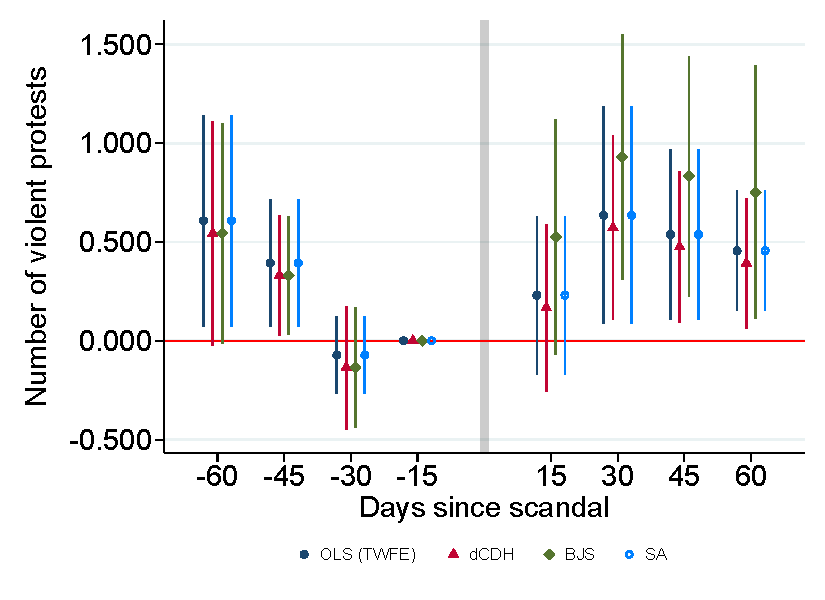
\includegraphics[width=\textwidth]{did_modern_stk_es_mm_violent_pa_w60.pdf}
    \end{subfigure}\hfill
    \begin{subfigure}{0.48\textwidth}
        \caption{Non-Apex.}
        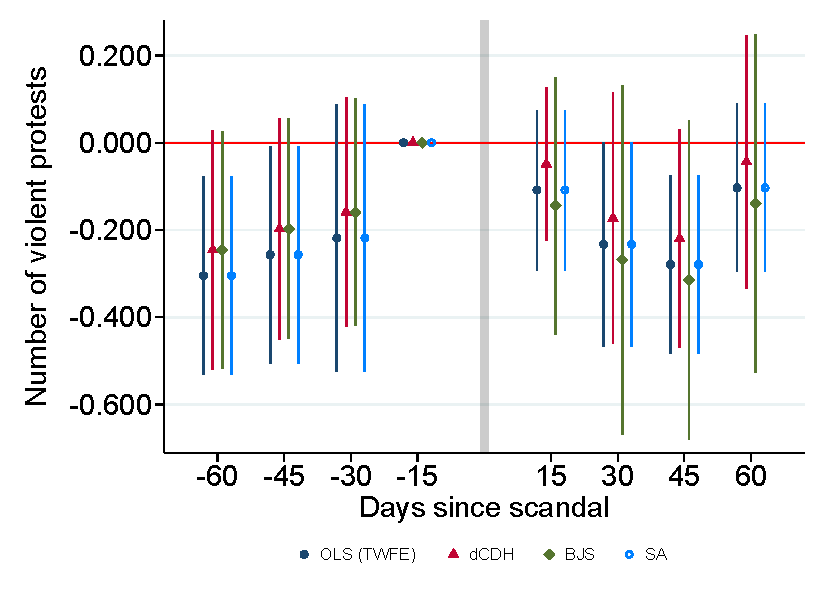
\includegraphics[width=\textwidth]{did_modern_stk_es_mm_violent_na_w60.pdf}
    \end{subfigure}
    \end{center}
    \footnotesize{Event-study coefficients on violent protests from four estimators---OLS two-way fixed effects (TWFE), de Chaisemartin--D'Haultf{\oe}uille (dCDH), Borusyak--Jaravel--Spiess (BJS), and Sun--Abraham (SA)---overlaid, on the Cengiz-style stacked-by-scandal panel (country $\times$ 15-day bin, $\pm 60$-day window; clean-control cohort $=$ countries with no scandal of any type in the window). The two panels are the Apex and Non-Apex subsamples; the time axis is in days (15-day bins) and the bin immediately before disclosure ($-1$) is the reference. Vertical bars are 90\% confidence intervals; standard errors clustered at the country level. Sample period 2008--2019; Venezuela excluded.}
\end{figure}

\begin{figure}[htb!]
    \caption{Modern DiD event studies (violent protests), stacked-by-scandal design, $\pm 90$-day window.}
    \label{fig:sup_did_stk_es_w90}
    \begin{center}
    \begin{subfigure}{0.48\textwidth}
        \caption{Apex.}
        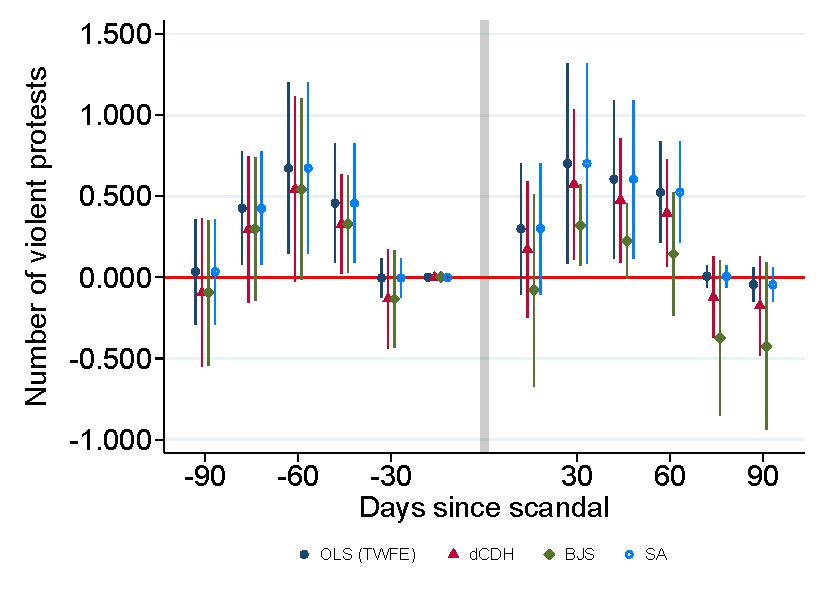
\includegraphics[width=\textwidth]{did_modern_stk_es_mm_violent_pa_w90.pdf}
    \end{subfigure}\hfill
    \begin{subfigure}{0.48\textwidth}
        \caption{Non-Apex.}
        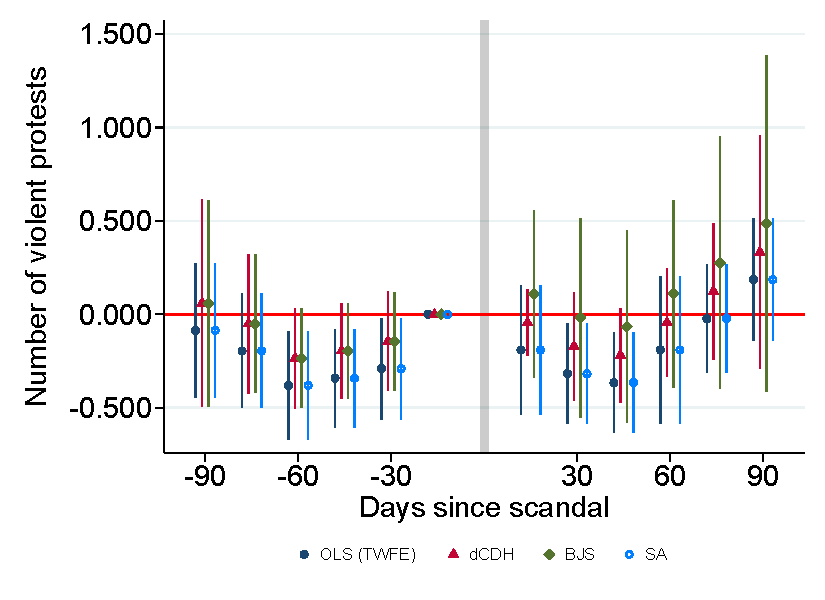
\includegraphics[width=\textwidth]{did_modern_stk_es_mm_violent_na_w90.pdf}
    \end{subfigure}
    \end{center}
    \footnotesize{Event-study coefficients on violent protests from four estimators---OLS TWFE, dCDH, BJS, and SA---overlaid, on the Cengiz-style stacked-by-scandal panel (country $\times$ 15-day bin, $\pm 90$-day window; clean-control cohort $=$ countries with no scandal of any type in the window). The two panels are the Apex and Non-Apex subsamples; time axis in days (15-day bins), reference bin $-1$. Vertical bars are 90\% confidence intervals; standard errors clustered at the country level. Sample period 2008--2019; Venezuela excluded.}
\end{figure}

\begin{figure}[htb!]
    \caption{Modern DiD event studies (violent protests), stacked-by-scandal design, $\pm 120$-day window.}
    \label{fig:sup_did_stk_es_w120}
    \begin{center}
    \begin{subfigure}{0.48\textwidth}
        \caption{Apex.}
        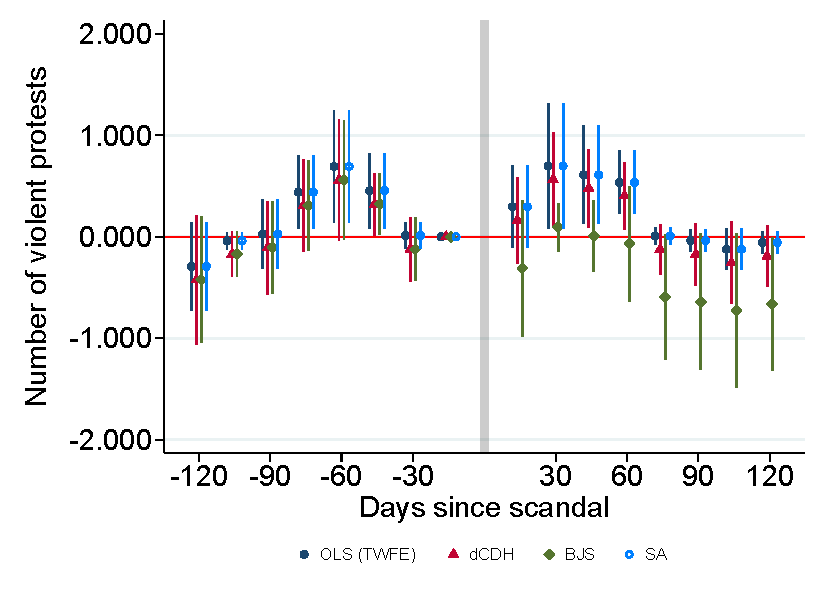
\includegraphics[width=\textwidth]{did_modern_stk_es_mm_violent_pa_w120.pdf}
    \end{subfigure}\hfill
    \begin{subfigure}{0.48\textwidth}
        \caption{Non-Apex.}
        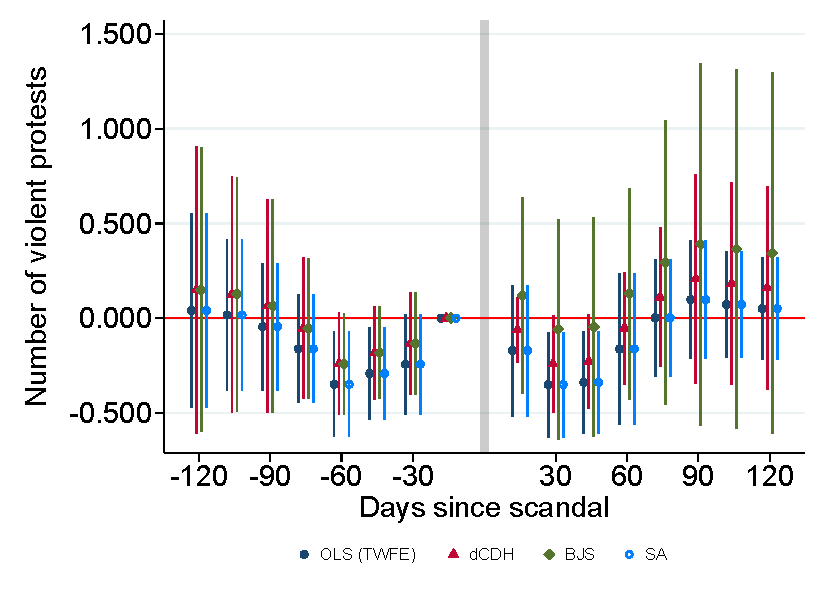
\includegraphics[width=\textwidth]{did_modern_stk_es_mm_violent_na_w120.pdf}
    \end{subfigure}
    \end{center}
    \footnotesize{Event-study coefficients on violent protests from four estimators---OLS TWFE, dCDH, BJS, and SA---overlaid, on the Cengiz-style stacked-by-scandal panel (country $\times$ 15-day bin, $\pm 120$-day window; clean-control cohort $=$ countries with no scandal of any type in the window). The two panels are the Apex and Non-Apex subsamples; time axis in days (15-day bins), reference bin $-1$. Vertical bars are 90\% confidence intervals; standard errors clustered at the country level. Sample period 2008--2019; Venezuela excluded.}
\end{figure}

\begin{table}[htb!]
    \caption{Modern DiD estimators, 15-day-bin staggered design.}
    \label{tab:sup_did_cw}
    \begin{center}\scriptsize
        \textbf{\textit{Panel A: Apex}}\\[3pt]
        {
\def\sym#1{\ifmmode^{#1}\else\(^{#1}\)\fi}
\begin{tabular}{l*{8}{c}}
\toprule
 & \multicolumn{4}{c}{Violent Protests} & \multicolumn{4}{c}{Non-violent Protests} \\
\cmidrule(lr){2-5}\cmidrule(lr){6-9}
 & \ensuremath{\pm 30} & \ensuremath{\pm 60} & \ensuremath{\pm 90} & \ensuremath{\pm 120} & \ensuremath{\pm 30} & \ensuremath{\pm 60} & \ensuremath{\pm 90} & \ensuremath{\pm 120} \\
\midrule
OLS (TWFE) & -0.244 & -0.244 & -0.244 & -0.244 & -0.027 & -0.027 & -0.027 & -0.027 \\
             & (0.180) & (0.180) & (0.180) & (0.180) & (0.168) & (0.168) & (0.168) & (0.168) \\
dCDH & 0.024 & 0.305 & 0.238 & 0.193 & 0.240 & 0.315 & 0.650 & 0.973 \\
             & (0.116) & (0.367) & (0.317) & (0.315) & (0.307) & (0.306) & (0.607) & (0.751) \\
BJS & -0.211 & -0.211 & -0.211 & -0.211 & -0.028 & -0.028 & -0.028 & -0.028 \\
             & (0.173) & (0.173) & (0.173) & (0.173) & (0.114) & (0.114) & (0.114) & (0.114) \\
SA & -0.461\sym{*} & -0.204 & -0.285 & -0.337 & -0.264 & -0.200 & 0.201 & 0.565 \\
             & (0.259) & (0.394) & (0.307) & (0.267) & (0.277) & (0.211) & (0.381) & (0.376) \\
\midrule
Observations & 6,453 & 6,453 & 6,453 & 6,453 & 6,453 & 6,453 & 6,453 & 6,453 \\
\bottomrule
\end{tabular}
}
\\[10pt]
        \textbf{\textit{Panel B: Non-Apex}}\\[3pt]
        {
\def\sym#1{\ifmmode^{#1}\else\(^{#1}\)\fi}
\begin{tabular}{l*{9}{c}}
\toprule
 & \multicolumn{3}{c}{Violent Protests} & \multicolumn{3}{c}{Non-violent Protests} & \multicolumn{3}{c}{Protests (any)} \\
\cmidrule(lr){2-4}\cmidrule(lr){5-7}\cmidrule(lr){8-10}
 & \ensuremath{\pm 60} & \ensuremath{\pm 90} & \ensuremath{\pm 120} & \ensuremath{\pm 60} & \ensuremath{\pm 90} & \ensuremath{\pm 120} & \ensuremath{\pm 60} & \ensuremath{\pm 90} & \ensuremath{\pm 120} \\
\midrule
OLS (TWFE) & -0.407 & -0.407 & -0.407 & 0.253 & 0.253 & 0.253 & -0.154 & -0.154 & -0.154 \\
             & (0.282) & (0.282) & (0.282) & (0.186) & (0.186) & (0.186) & (0.266) & (0.266) & (0.266) \\
dCDH & 0.150 & 0.163 & 0.178 & -0.399 & -0.461 & -0.519 & -0.249 & -0.298 & -0.341 \\
             & (0.094) & (0.107) & (0.123) & (0.511) & (0.635) & (0.693) & (0.520) & (0.627) & (0.672) \\
BJS & -0.466\sym{**} & -0.466\sym{**} & -0.466\sym{**} & 0.048 & 0.048 & 0.048 & -0.419 & -0.419 & -0.419 \\
             & (0.222) & (0.222) & (0.222) & (0.085) & (0.085) & (0.085) & (0.263) & (0.263) & (0.263) \\
SA & -0.081 & -0.110\sym{*} & -0.133\sym{**} & 0.085 & 0.030 & -0.021 & 0.004 & -0.080 & -0.154 \\
             & (0.066) & (0.058) & (0.059) & (0.309) & (0.216) & (0.170) & (0.319) & (0.230) & (0.186) \\
\midrule
Observations & 6,752 & 6,752 & 6,752 & 6,752 & 6,752 & 6,752 & 6,752 & 6,752 & 6,752 \\
\bottomrule
\end{tabular}
}

    \end{center}
    \footnotesize{Static post-treatment coefficient (standard error) from four estimators---OLS two-way fixed effects (TWFE), de Chaisemartin--D'Haultf{\oe}uille (dCDH), Borusyak--Jaravel--Spiess (BJS), and Sun--Abraham (SA)---on the country $\times$ 15-day-bin staggered panel, with treatment defined as each country's first-scandal bin. The control cohort is restricted to country-years with no scandal of any type, and protest counts are zero on no-protest days. Columns are two Mass-Mobilization outcomes---violent protests and non-violent protests---each at the $\pm 30$-, $\pm 60$-, $\pm 90$-, and $\pm 120$-day windows (2/4/6/8 bins per side). Standard errors clustered at the country level. Sample period 2008--2019; Venezuela excluded. Significance: $^{*}$ $p<0.1$, $^{**}$ $p<0.05$, $^{***}$ $p<0.01$.}
\end{table}

\begin{figure}[htb!]
    \caption{Modern DiD event studies (violent protests), 15-day bins, $\pm 60$-day window.}
    \label{fig:sup_did_cw_es}
    \begin{center}
    \begin{subfigure}{0.48\textwidth}
        \caption{Apex.}
        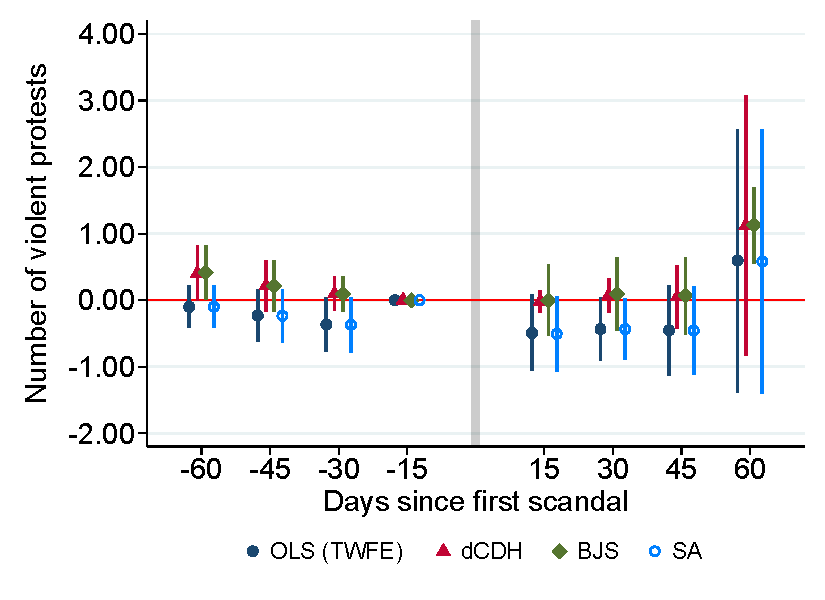
\includegraphics[width=\textwidth]{did_modern_es_mm_violent_pa_w60.pdf}
    \end{subfigure}\hfill
    \begin{subfigure}{0.48\textwidth}
        \caption{Non-Apex.}
        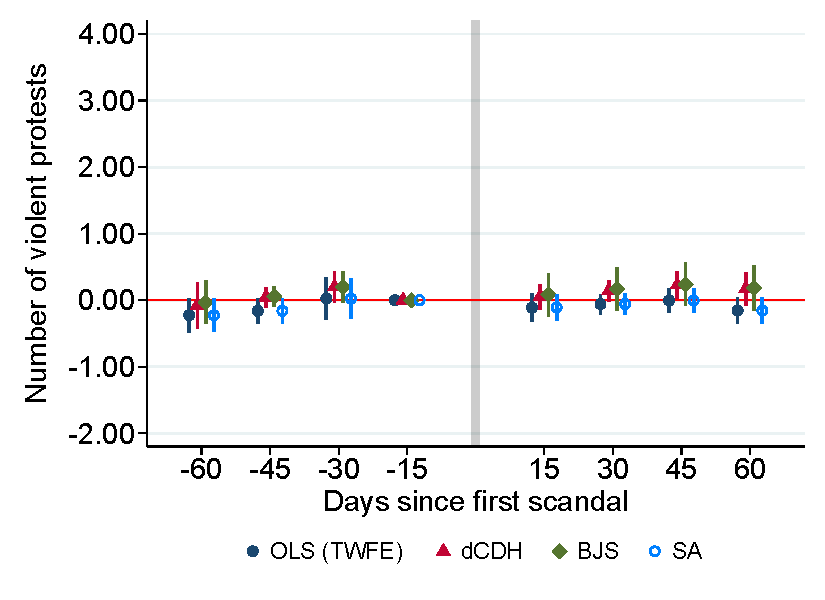
\includegraphics[width=\textwidth]{did_modern_es_mm_violent_na_w60.pdf}
    \end{subfigure}
    \end{center}
    \footnotesize{Event-study coefficients on violent protests from four estimators---OLS two-way fixed effects (TWFE), de Chaisemartin--D'Haultf{\oe}uille (dCDH), Borusyak--Jaravel--Spiess (BJS), and Sun--Abraham (SA)---overlaid, estimated on the country $\times$ 15-day-bin staggered panel with treatment defined as each country's first-scandal bin (never-treated cohort $=$ countries with no subsample scandal), at the $\pm 60$-day window (4 bins per side). The two panels are the Apex and Non-Apex subsamples; the time axis is in days (15-day bins) and the bin immediately before disclosure ($-1$, the 15 days before disclosure) is the reference. Vertical bars are 90\% confidence intervals; standard errors clustered at the country level. Sample period 2008--2019; Venezuela excluded.}
\end{figure}

\begin{figure}[htb!]
    \caption{Modern DiD event studies (violent protests), 15-day bins, $\pm 90$-day window.}
    \label{fig:sup_did_cw_es_w90}
    \begin{center}
    \begin{subfigure}{0.48\textwidth}
        \caption{Apex.}
        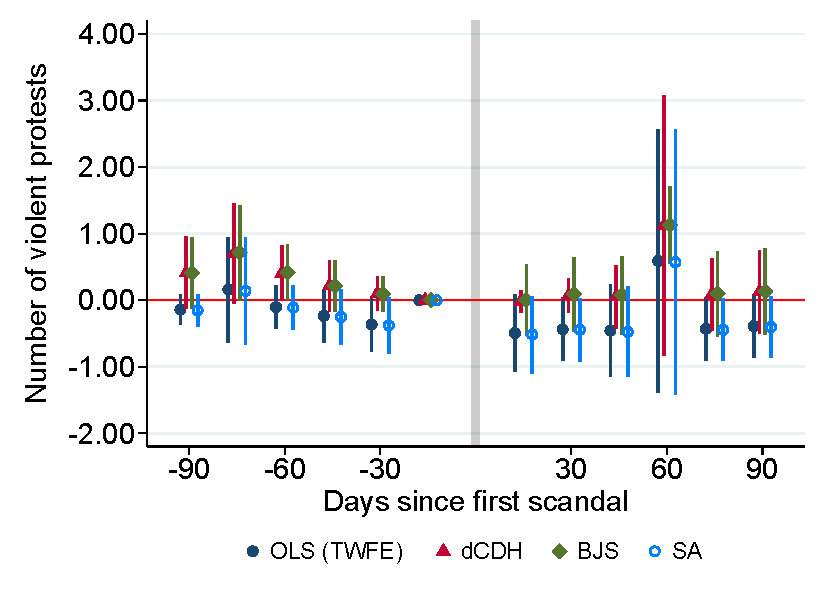
\includegraphics[width=\textwidth]{did_modern_es_mm_violent_pa_w90.pdf}
    \end{subfigure}\hfill
    \begin{subfigure}{0.48\textwidth}
        \caption{Non-Apex.}
        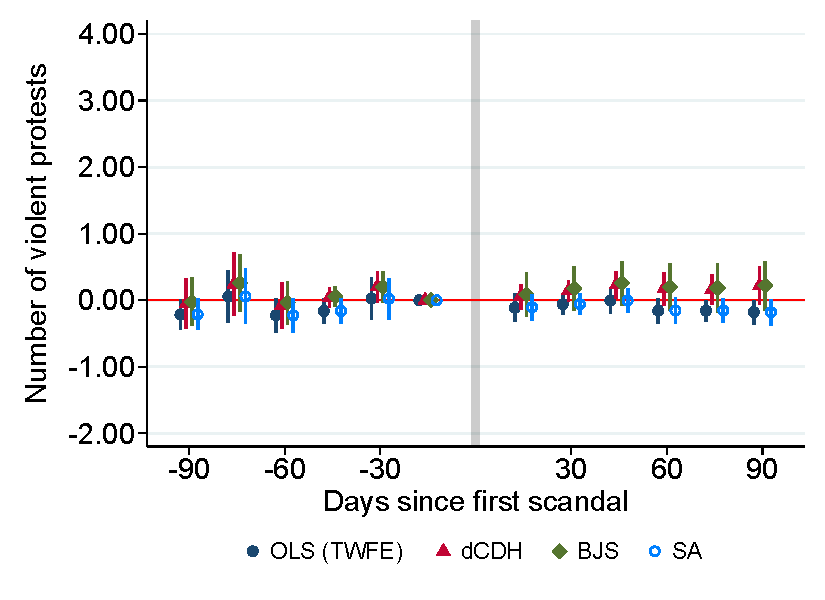
\includegraphics[width=\textwidth]{did_modern_es_mm_violent_na_w90.pdf}
    \end{subfigure}
    \end{center}
    \footnotesize{Event-study coefficients on violent protests from four estimators---OLS TWFE, dCDH, BJS, and SA---overlaid, estimated on the country $\times$ 15-day-bin staggered panel with treatment defined as each country's first-scandal bin, at the $\pm 90$-day window (6 bins per side). The two panels are the Apex and Non-Apex subsamples; the time axis is in days (15-day bins) and the bin immediately before disclosure ($-1$) is the reference. Vertical bars are 90\% confidence intervals; standard errors clustered at the country level. Sample period 2008--2019; Venezuela excluded.}
\end{figure}

\begin{figure}[htb!]
    \caption{Modern DiD event studies (violent protests), 15-day bins, $\pm 120$-day window.}
    \label{fig:sup_did_cw_es_w120}
    \begin{center}
    \begin{subfigure}{0.48\textwidth}
        \caption{Apex.}
        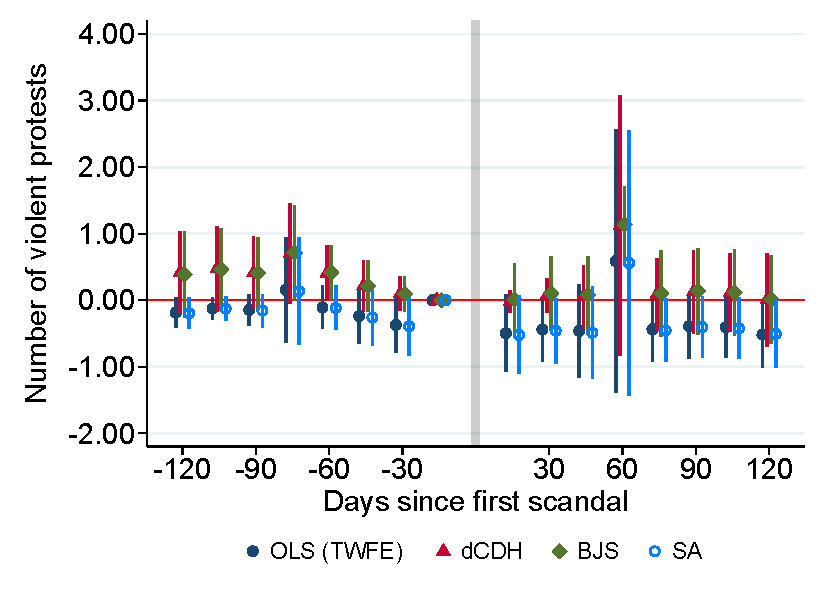
\includegraphics[width=\textwidth]{did_modern_es_mm_violent_pa_w120.pdf}
    \end{subfigure}\hfill
    \begin{subfigure}{0.48\textwidth}
        \caption{Non-Apex.}
        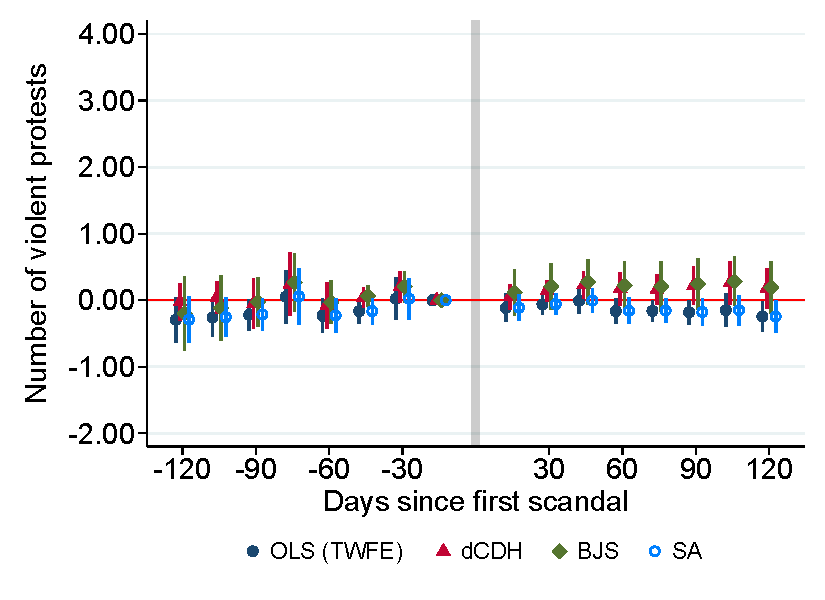
\includegraphics[width=\textwidth]{did_modern_es_mm_violent_na_w120.pdf}
    \end{subfigure}
    \end{center}
    \footnotesize{Event-study coefficients on violent protests from four estimators---OLS TWFE, dCDH, BJS, and SA---overlaid, estimated on the country $\times$ 15-day-bin staggered panel with treatment defined as each country's first-scandal bin, at the $\pm 120$-day window (8 bins per side). The two panels are the Apex and Non-Apex subsamples; the time axis is in days (15-day bins) and the bin immediately before disclosure ($-1$) is the reference. Vertical bars are 90\% confidence intervals; standard errors clustered at the country level. Sample period 2008--2019; Venezuela excluded.}
\end{figure}

% ---------------------------------------------------------------------
% \clearpage
% \section{Pooled event study and per-scandal heterogeneity by rank}\label{sup:pooled_box}

% Figure~\ref{fig:sup_eventstudies_full} shows the event study pooling all 176 scandals (rather than splitting by subsample). Figure~\ref{fig:sup_boxplots} summarizes the finer within-apex gradient: we estimate \autoref{eq:main} for each scandal on its own country's $\pm$30-day window and plot, by box plot, the cross-scandal distribution of the per-scandal coefficients under the three-way partition. The median per-scandal violent-protest effect for Presidents is an order of magnitude larger than for the Other Apex category, which is in turn larger than for Non-Apex---a descriptive comparison that rests on the subset of scandals with within-window variation in the outcome.

% \begin{figure}[htb!]
%     \caption{Pooled event study (all 176 scandals), $\pm 120$-day window (30-day bins).}
%     \label{fig:sup_eventstudies_full}
%     \begin{subfigure}{0.45\textwidth}
%         \caption{Violent protests.}
%         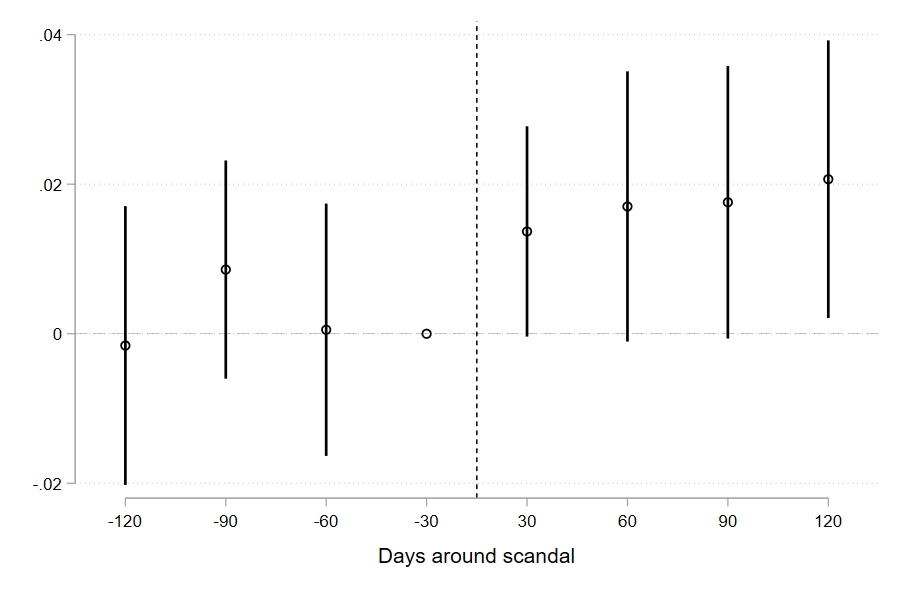
\includegraphics[width=\textwidth]{es_num_violent_MM_120d_90ci.png}
%     \end{subfigure}\hfill
%     \begin{subfigure}{0.45\textwidth}
%         \caption{Peaceful protests.}
%         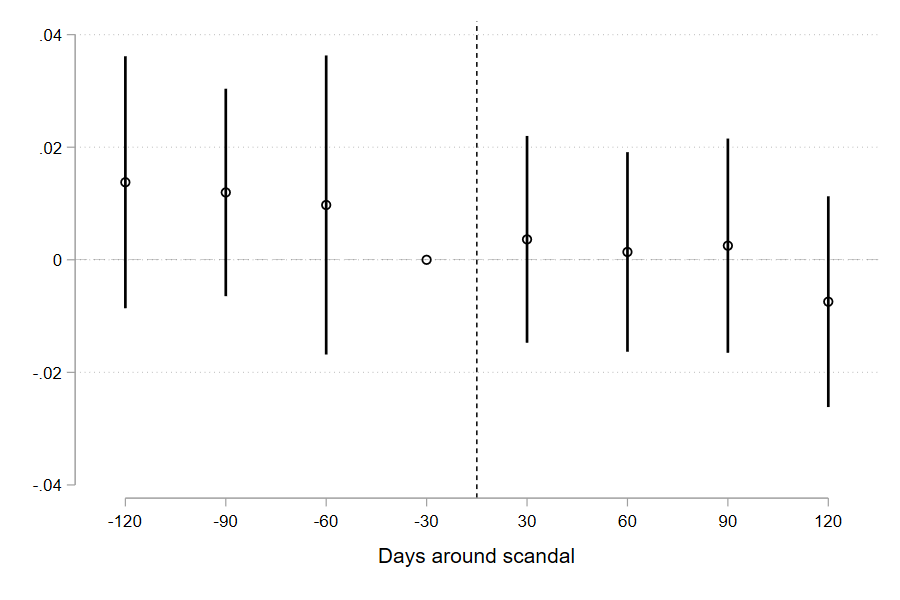
\includegraphics[width=\textwidth]{es_num_peaceful_MM_120d_90ci.png}
%     \end{subfigure}
%     \footnotesize{Event-time 30-day-bin coefficients from the modified \autoref{eq:main} on all scandals pooled; omitted bin is the 30 days before disclosure. Vertical bars are 90\% confidence intervals. An observation is a country-scandal-date. Sample period 2008--2019; Venezuela excluded.}
% \end{figure}

% \begin{figure}[htb!]
%     \caption{Per-scandal effects by political rank.}
%     \label{fig:sup_boxplots}
%     \begin{center}
%         \begin{subfigure}{0.485\textwidth}
%             \caption{Violent protests.}
%             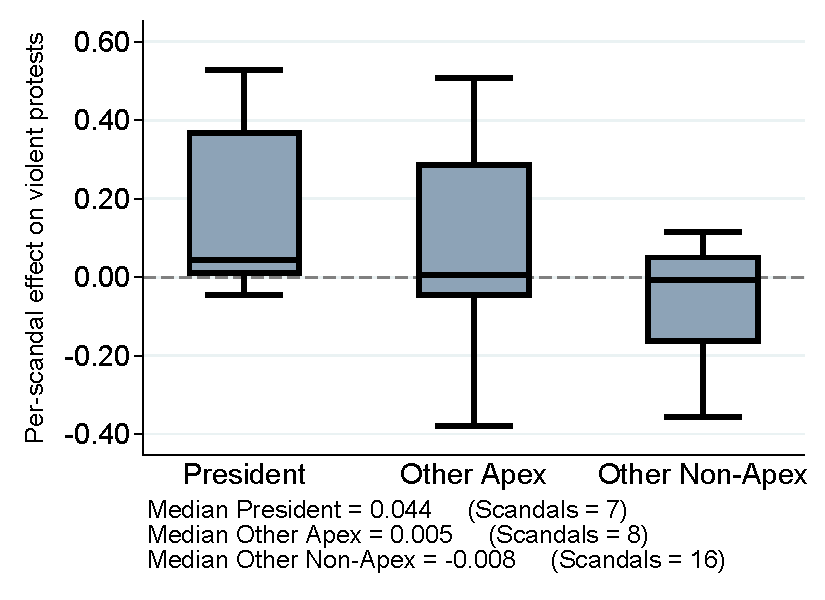
\includegraphics[width=\textwidth]{per_scandal_box_num_violent_MM_w30_apex_v2.pdf}
%         \end{subfigure}\hfill
%         \begin{subfigure}{0.485\textwidth}
%             \caption{Peaceful protests.}
%             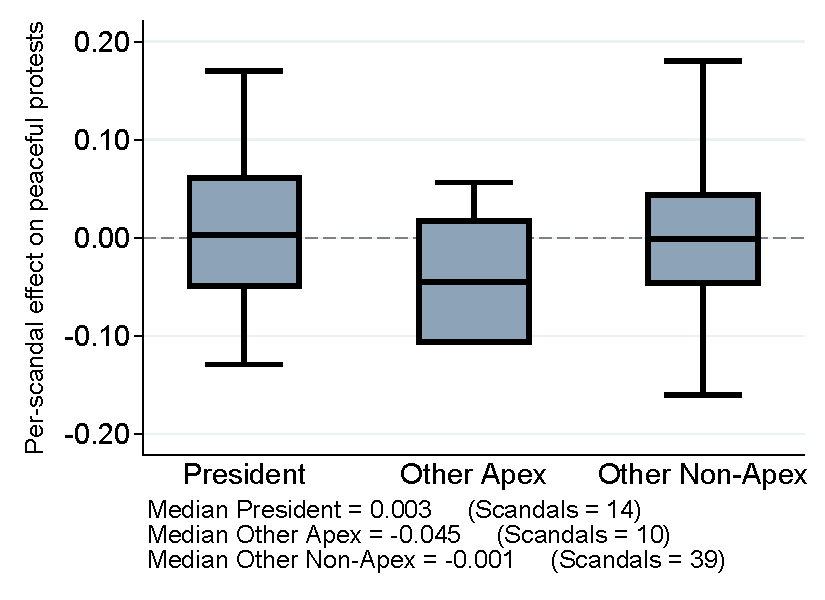
\includegraphics[width=\textwidth]{per_scandal_box_num_peaceful_MM_w30_apex_v2.pdf}
%         \end{subfigure}
%     \end{center}
%     \footnotesize{We estimate the OLS post-scandal coefficient of \autoref{eq:main} on the $\pm$30-day window of each implicated country alone (retaining day-of-week and month-of-year fixed effects). Each panel box-plots the cross-scandal distribution of those per-scandal coefficients under the apex partition of \autoref{sup:classification}: President (45), Other Apex (19), Non-Apex (112). Scandals with no within-window variation in the outcome are dropped from the corresponding box plot. Sample period 2008--2019; Venezuela excluded.}
% \end{figure}

% ---------------------------------------------------------------------
\clearpage
\section{Selection-on-observables DiD: regression adjustment and reweighting}\label{sup:did_ra}

As a transparent complement to the heterogeneity-robust estimators of \autoref{sup:did}, we condition on the pre-scandal outcome dynamics directly, in the spirit of Acemoglu, Naidu, Restrepo and Robinson~\citep{acemoglu2019DemoEcoGrowth}. \autoref{tab:sup_did_ra} reports the static (windowed) post-scandal effect from four nested specifications on the country $\times$ 15-day-bin staggered panel: no adjustment (two-way fixed effects), regression adjustment (adding four lags of the outcome), inverse-propensity weighting (reweighting the clean controls by their propensity of being a treated country given a baseline protest covariate), and doubly robust (both). \autoref{fig:sup_did_ra_es} plots the corresponding violent-protest event studies. The apex effect is stable across all four adjustments and the pre-trend test is insignificant throughout.

\begin{table}[htb!]
    \caption{Selection-on-observables DiD: windowed ATT and pre-trend test.}
    \label{tab:sup_did_ra}
    \begin{center}\scriptsize
        \textbf{Apex sample}\\[3pt]
        {
\def\sym#1{\ifmmode^{#1}\else\(^{#1}\)\fi}
\begin{tabular}{l*{6}{c}}
\toprule
 & \multicolumn{3}{c}{Violent Protests} & \multicolumn{3}{c}{Non-violent Protests} \\
\cmidrule(lr){2-4}\cmidrule(lr){5-7}
 & \ensuremath{\pm 60} & \ensuremath{\pm 90} & \ensuremath{\pm 120} & \ensuremath{\pm 60} & \ensuremath{\pm 90} & \ensuremath{\pm 120} \\
\midrule
\multicolumn{7}{l}{\textit{Panel A: windowed ATT (average post-scandal effect)}}\\
No adjustment & 0.283 & 0.272 & 0.229 & 0.302 & 0.678 & 1.048 \\
             & (0.417) & (0.400) & (0.417) & (0.312) & (0.568) & (0.725) \\
Regression adj. & 0.470 & 0.277 & 0.217 & 0.159 & 0.485 & 0.544 \\
             & (0.369) & (0.275) & (0.262) & (0.146) & (0.383) & (0.360) \\
IPW & 0.335 & 0.229 & 0.147 & 0.363 & 0.757 & 1.131 \\
             & (0.315) & (0.209) & (0.166) & (0.244) & (0.533) & (0.709) \\
Doubly robust & 0.338 & 0.114 & 0.048 & 0.183 & 0.520 & 0.595 \\
             & (0.290) & (0.098) & (0.059) & (0.144) & (0.394) & (0.384) \\
\midrule
\multicolumn{7}{l}{\textit{Panel B: pre-trend test, \(p\)-value (joint: all lead coefficients \(=0\))}}\\
No adjustment & 0.483 & 0.548 & 0.763 & 0.761 & 0.376 & 0.276 \\
Regression adj. & 0.858 & 0.628 & 0.759 & 0.941 & 0.319 & 0.390 \\
IPW & 0.272 & 0.302 & 0.433 & 0.785 & 0.429 & 0.320 \\
Doubly robust & 0.860 & 0.370 & 0.076 & 0.940 & 0.283 & 0.395 \\
\bottomrule
\end{tabular}
}
\\[10pt]
        \textbf{Non-Apex sample}\\[3pt]
        {
\def\sym#1{\ifmmode^{#1}\else\(^{#1}\)\fi}
\begin{tabular}{l*{6}{c}}
\toprule
 & \multicolumn{3}{c}{Violent Protests} & \multicolumn{3}{c}{Non-violent Protests} \\
\cmidrule(lr){2-4}\cmidrule(lr){5-7}
 & \ensuremath{\pm 60} & \ensuremath{\pm 90} & \ensuremath{\pm 120} & \ensuremath{\pm 60} & \ensuremath{\pm 90} & \ensuremath{\pm 120} \\
\midrule
\multicolumn{7}{l}{\textit{Panel A: windowed ATT (average post-scandal effect)}}\\
No adjustment & 0.130 & 0.106 & 0.079 & -0.278 & -0.350 & -0.396 \\
             & (0.176) & (0.185) & (0.162) & (0.542) & (0.672) & (0.716) \\
Regression adj. & 0.219 & 0.200 & 0.179 & -0.006 & 0.039 & 0.063 \\
             & (0.203) & (0.196) & (0.170) & (0.364) & (0.369) & (0.378) \\
IPW & 0.133 & 0.108 & 0.092 & -0.045 & -0.095 & -0.144 \\
             & (0.179) & (0.189) & (0.178) & (0.713) & (0.832) & (0.871) \\
Doubly robust & 0.213 & 0.193 & 0.181 & 0.094 & 0.111 & 0.117 \\
             & (0.208) & (0.202) & (0.184) & (0.516) & (0.533) & (0.527) \\
\midrule
\multicolumn{7}{l}{\textit{Panel B: pre-trend test, \(p\)-value (joint: all lead coefficients \(=0\))}}\\
No adjustment & 0.209 & 0.439 & 0.602 & 0.232 & 0.262 & 0.232 \\
Regression adj. & 0.275 & 0.536 & 0.377 & 0.124 & 0.255 & 0.404 \\
IPW & 0.239 & 0.481 & 0.622 & 0.345 & 0.409 & 0.317 \\
Doubly robust & 0.321 & 0.584 & 0.453 & 0.159 & 0.259 & 0.441 \\
\bottomrule
\end{tabular}
}

    \end{center}
    \footnotesize{Windowed post-scandal ATT (Panel A) and the joint pre-trend $p$-value (Panel B, testing that all pre-period lead coefficients are zero) from four specifications---no adjustment (TWFE), regression adjustment (four outcome lags), inverse-propensity weighting, and doubly robust---on the country $\times$ 15-day-bin staggered panel (treatment $=$ each country's first-scandal bin; clean controls $=$ scandal-free country-years). Columns are violent and non-violent protests at the $\pm 60$/$\pm 90$/$\pm 120$-day windows. Standard errors clustered at the country level. Sample period 2008--2019; Venezuela excluded. Significance: $^{*}$ $p<0.1$, $^{**}$ $p<0.05$, $^{***}$ $p<0.01$.}
\end{table}

\begin{figure}[htb!]
    \caption{Selection-on-observables DiD event studies (violent protests, $\pm 60$-day window).}
    \label{fig:sup_did_ra_es}
    \begin{center}
    \begin{subfigure}{0.48\textwidth}\caption{Apex.}
        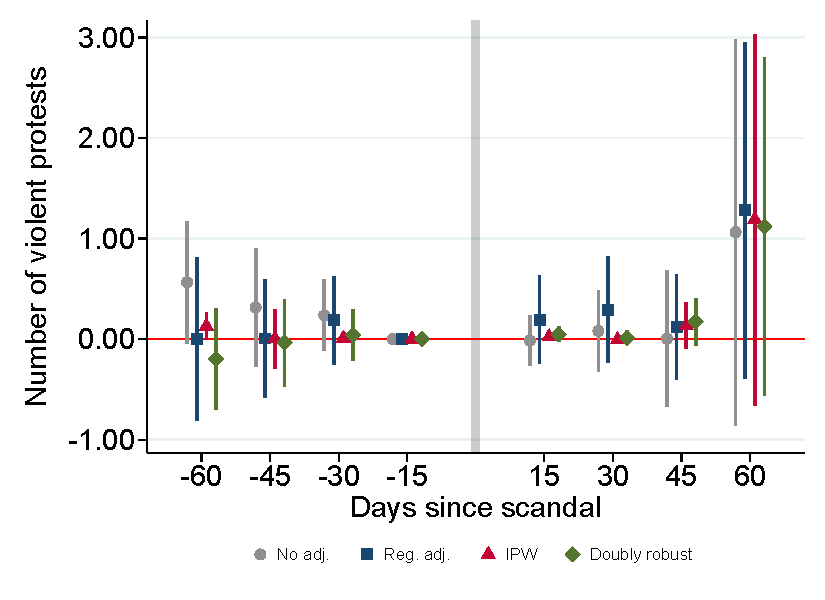
\includegraphics[width=\textwidth]{did_ra_es_mm_violent_pa_w60.pdf}\end{subfigure}\hfill
    \begin{subfigure}{0.48\textwidth}\caption{Non-Apex.}
        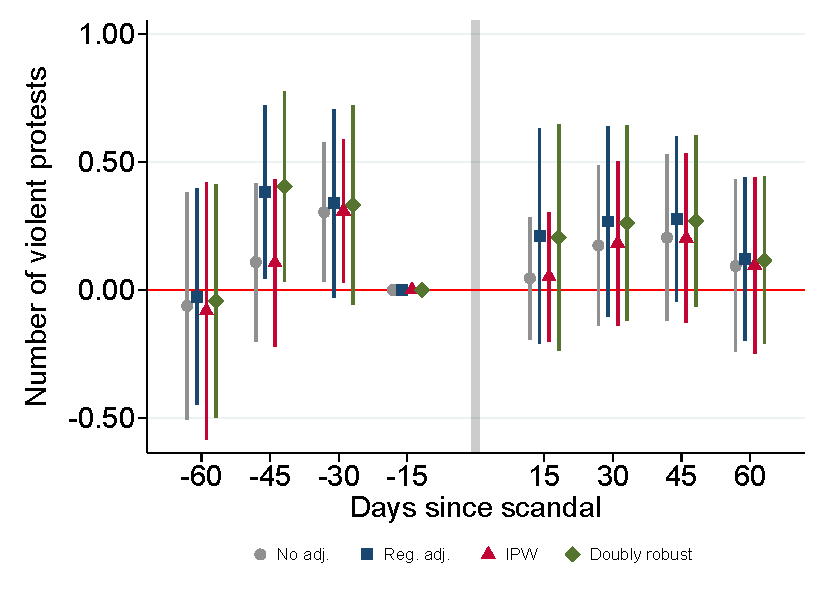
\includegraphics[width=\textwidth]{did_ra_es_mm_violent_na_w60.pdf}\end{subfigure}
    \end{center}
    \footnotesize{Violent-protest event studies overlaying the four specifications---no adjustment, regression adjustment (four outcome lags), IPW, and doubly robust---on the country $\times$ 15-day-bin staggered panel, $\pm 60$-day window; the bin immediately before disclosure ($-1$) is the reference. Vertical bars are 90\% confidence intervals; standard errors clustered at the country level. Sample period 2008--2019; Venezuela excluded.}
\end{figure}
\end{comment}



% ---------------------------------------------------------------------
\clearpage
\section{Leave-one-out robustness by scandal}\label{sup:loo}

We re-estimate the two interaction coefficients on violent protests in the $\pm$30-day window, dropping one scandal's event window at a time, split by scandal type (Apex vs.\ Non-Apex, \autoref{fig:sup_loo}). No single scandal drives its coefficient---the leave-one-out estimates cluster tightly on the full-sample line (red). For the apex effect, removing the single most influential scandal lowers $\beta_{\text{Apex}}$ from about 0.048 to 0.029 but leaves it clearly positive. The two panels share a common vertical axis so the magnitudes are directly comparable.

\begin{figure}[htb!]
    \caption{Leave-one-out by scandal type.}
    \label{fig:sup_loo}
    \begin{center}
    \begin{subfigure}{\textwidth}
        \caption{Apex: $\beta_{\text{Apex}}$ (Post $\times$ Apex), dropping each apex scandal.}
        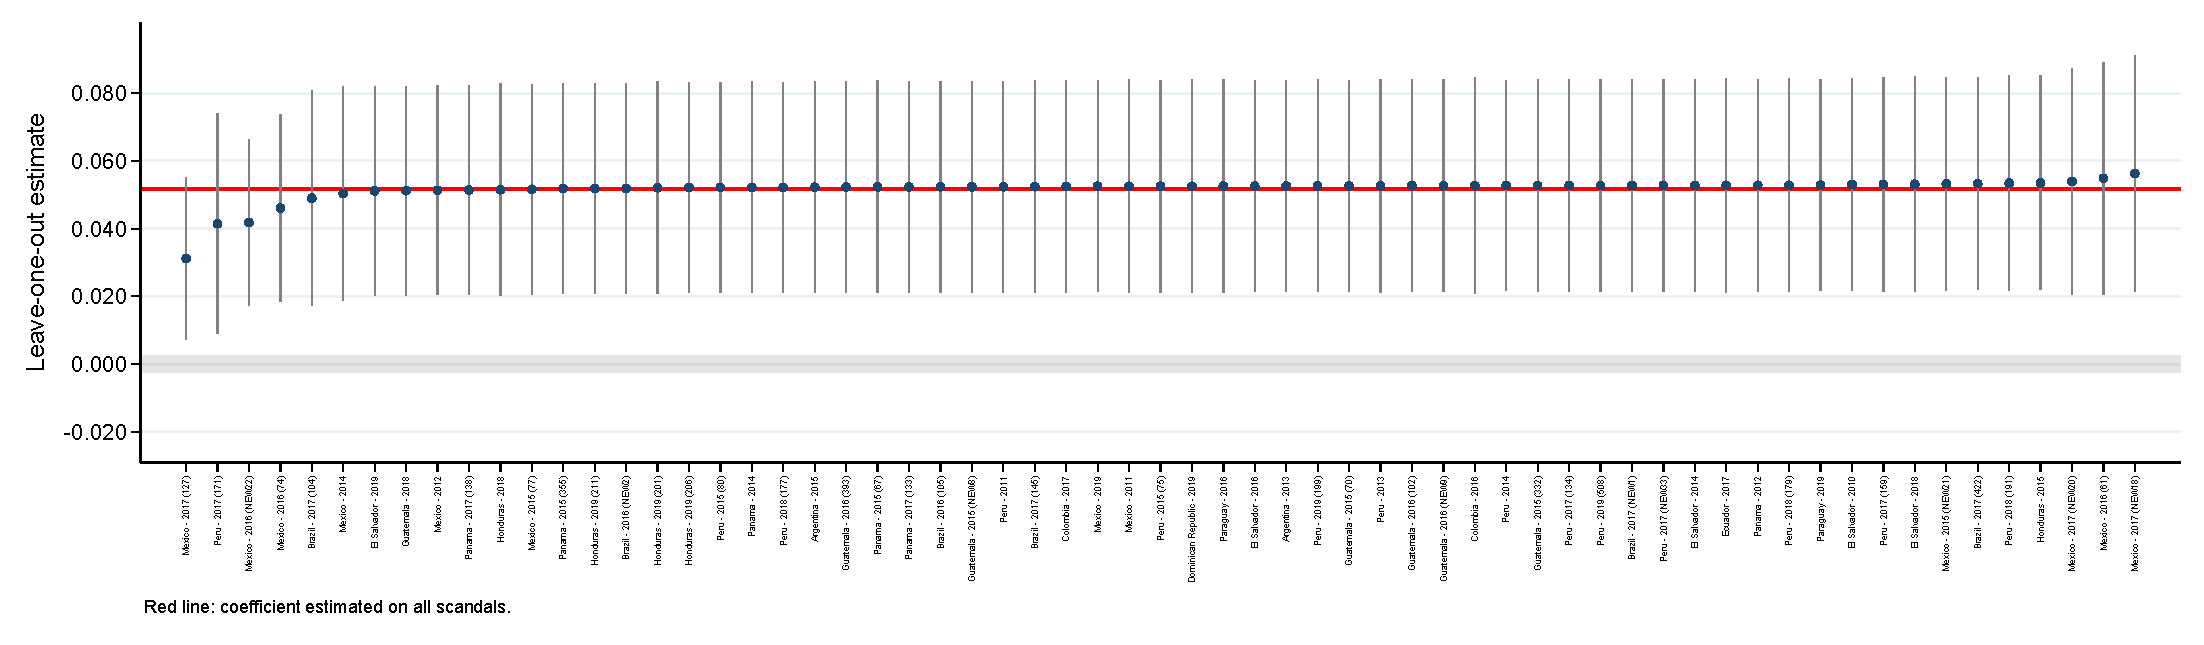
\includegraphics[width=\textwidth]{loo_scandal_beta_apex_violent_w30.pdf}
    \end{subfigure} \\[6pt]
    \begin{subfigure}{\textwidth}
        \caption{Non-Apex: $\beta_{\text{Non-Apex}}$ (Post $\times$ Non-Apex), dropping each non-apex scandal.}
        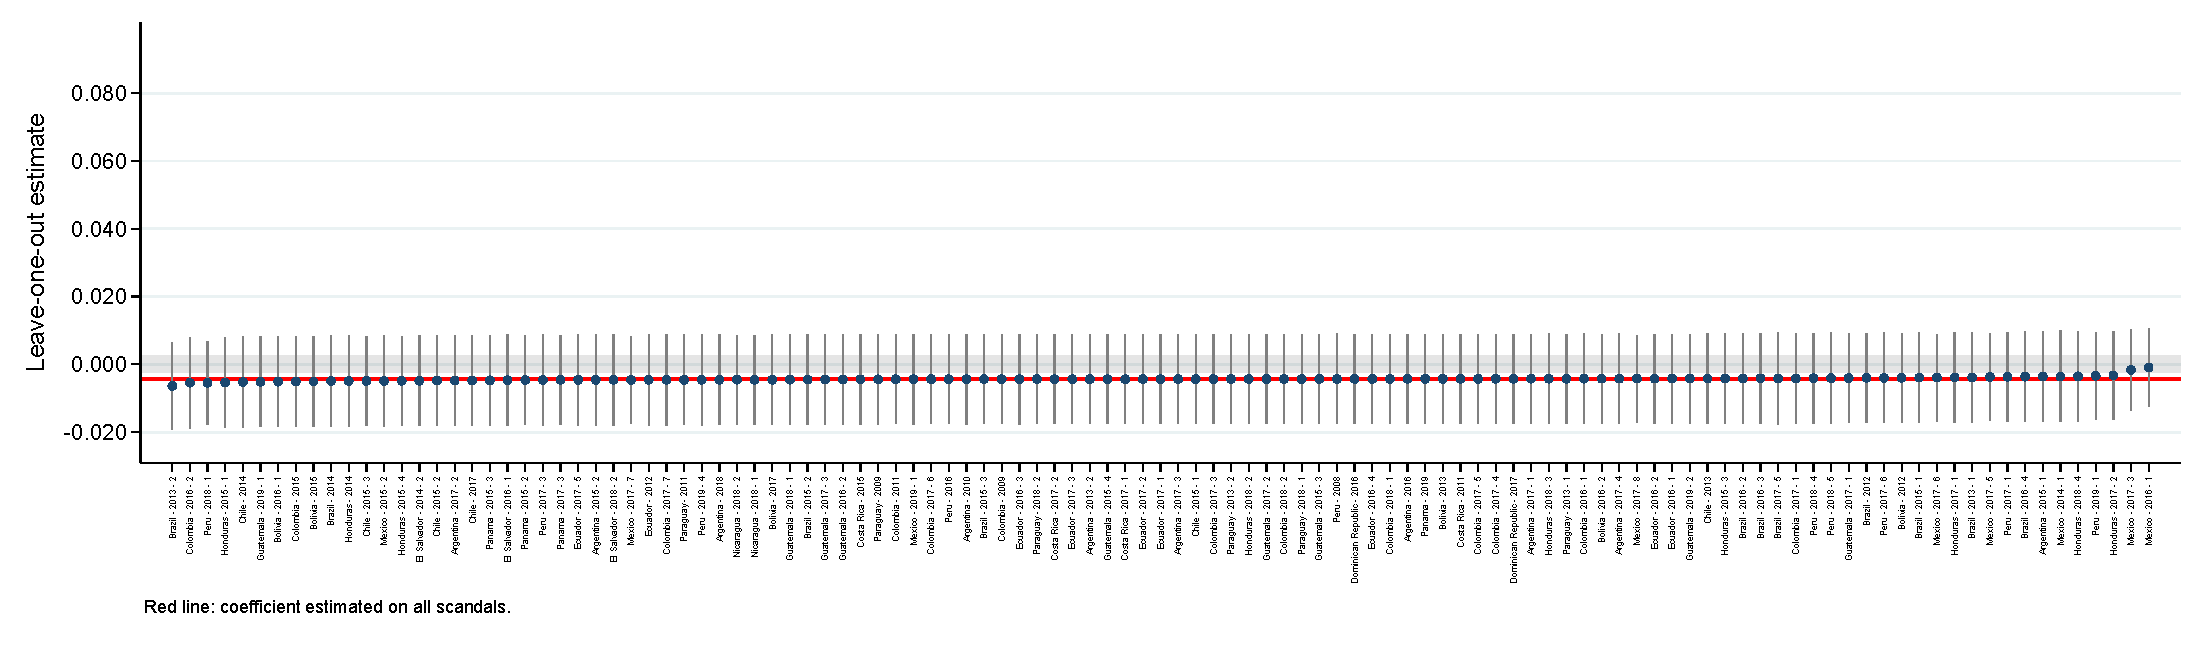
\includegraphics[width=\textwidth]{loo_scandal_beta_nonapex_violent_w30.pdf}
    \end{subfigure}
    \end{center}
    \footnotesize{Leave-one-out estimates of the two-group interaction coefficients (\autoref{tab:interaction}) on violent protests, $\pm 30$-day window. Each point re-estimates the panel's coefficient---Post $\times$ Apex in (a), Post $\times$ Non-Apex in (b)---dropping the labelled scandal's event window; panel (a) leaves out each of the 63 apex scandals, panel (b) each of the 113 non-apex scandals. Vertical bars are 90\% confidence intervals; scandals (x-axis, labelled Country -- Year, with a trailing ordinal ordering scandals by date within a country-year when there is more than one, e.g.\ ``Peru -- 2017 -- 3'') are sorted by the estimate. The red line is the coefficient on all scandals and the faint line marks zero; the two panels share a common vertical scale. Standard errors clustered at country $\times$ year $\times$ day-bin. Sample period 2008--2019; Venezuela excluded.}
\end{figure}

% ---------------------------------------------------------------------
\clearpage
\begin{comment}
\begin{figure}[htb!]
    \caption{Leave-one-out by rank hierarchy (as in Table~\ref{tab:sup_hierarchy}).}
    \label{fig:sup_loo_hier}
    \begin{center}
    \begin{subfigure}{\textwidth}
        \caption{President: $\beta_{\text{President}}$, dropping each Presidential scandal.}
        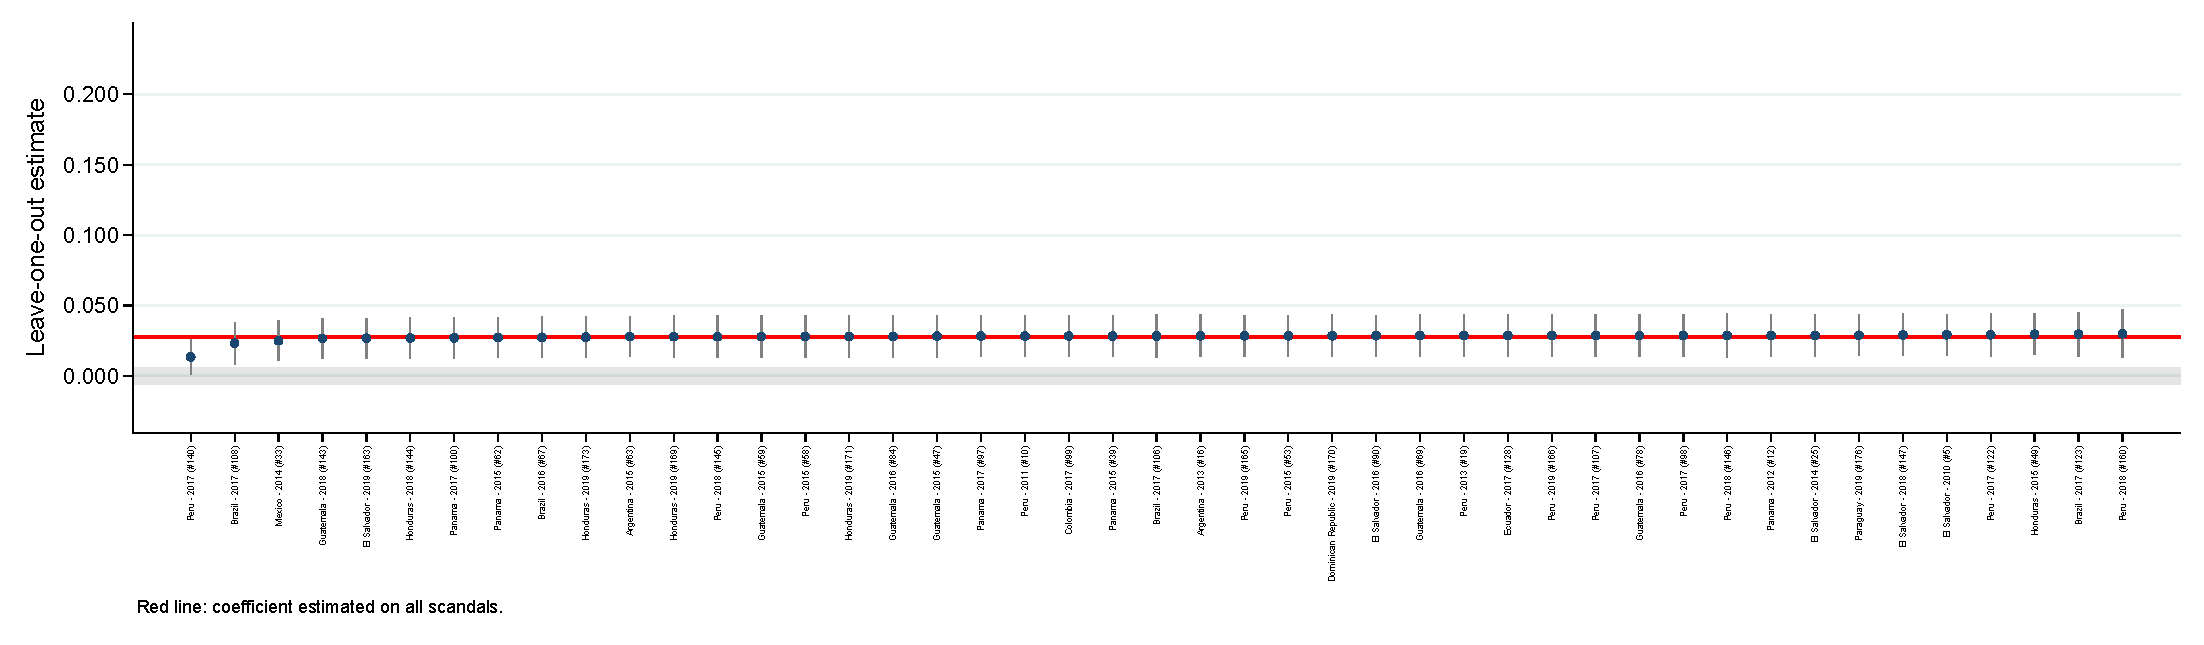
\includegraphics[width=\textwidth]{loo_scandal_beta_pres_violent_w30.pdf}
    \end{subfigure} \\[4pt]
    \begin{subfigure}{\textwidth}
        \caption{Other Apex: $\beta_{\text{Other Apex}}$, dropping each Other-Apex scandal.}
        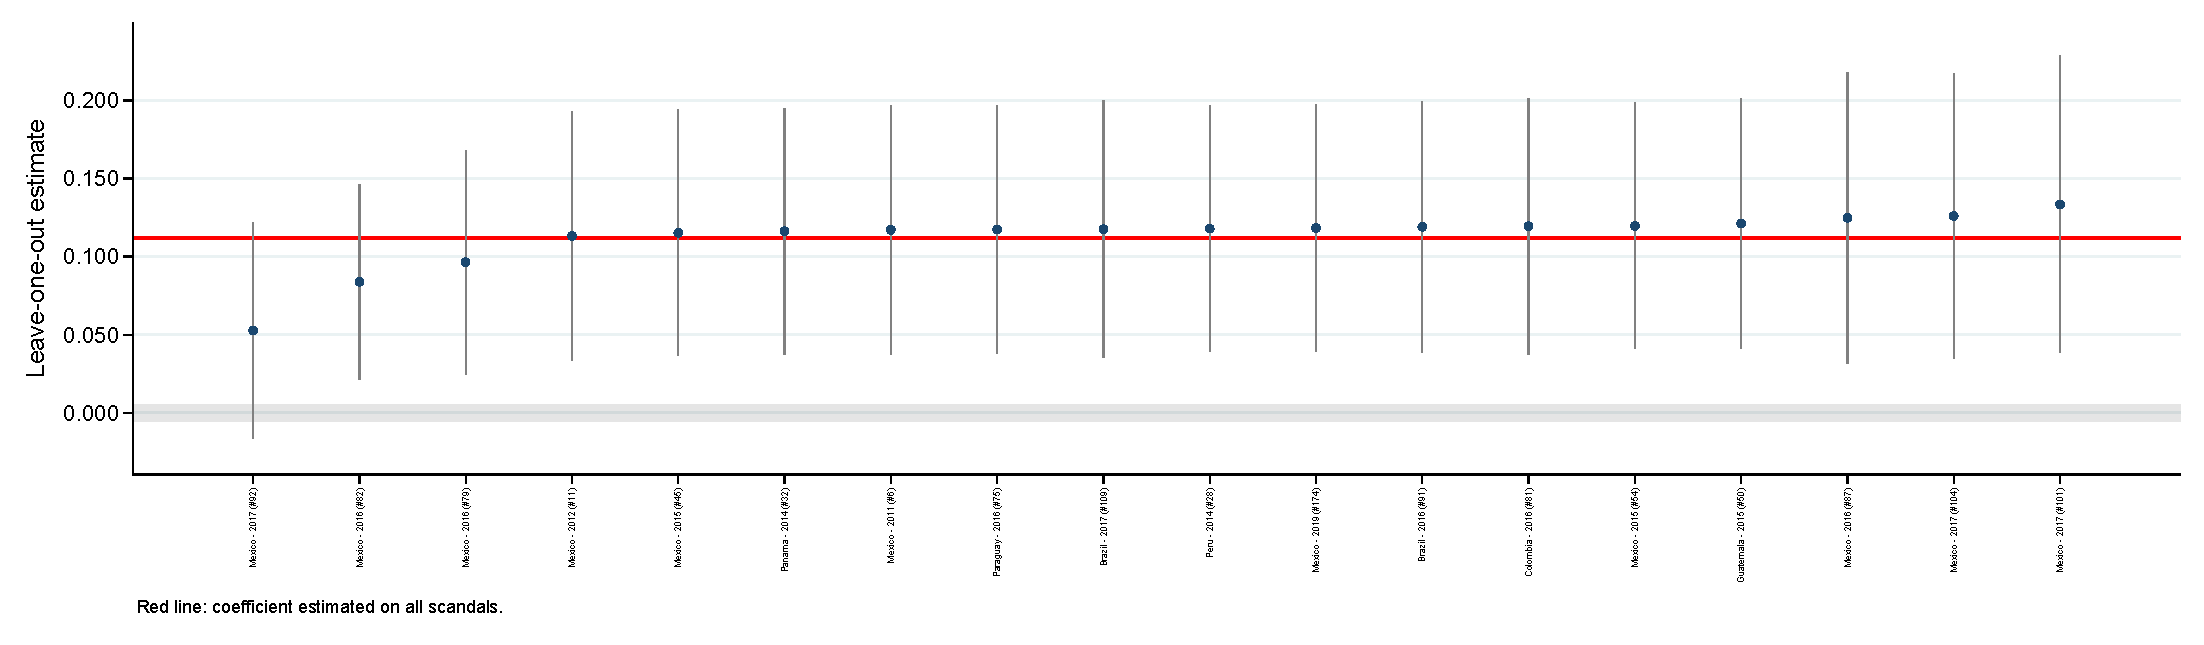
\includegraphics[width=\textwidth]{loo_scandal_beta_oa_violent_w30.pdf}
    \end{subfigure} \\[4pt]
    \begin{subfigure}{\textwidth}
        \caption{Other Non-Apex: $\beta_{\text{Other Non-Apex}}$, dropping each Non-Apex scandal.}
        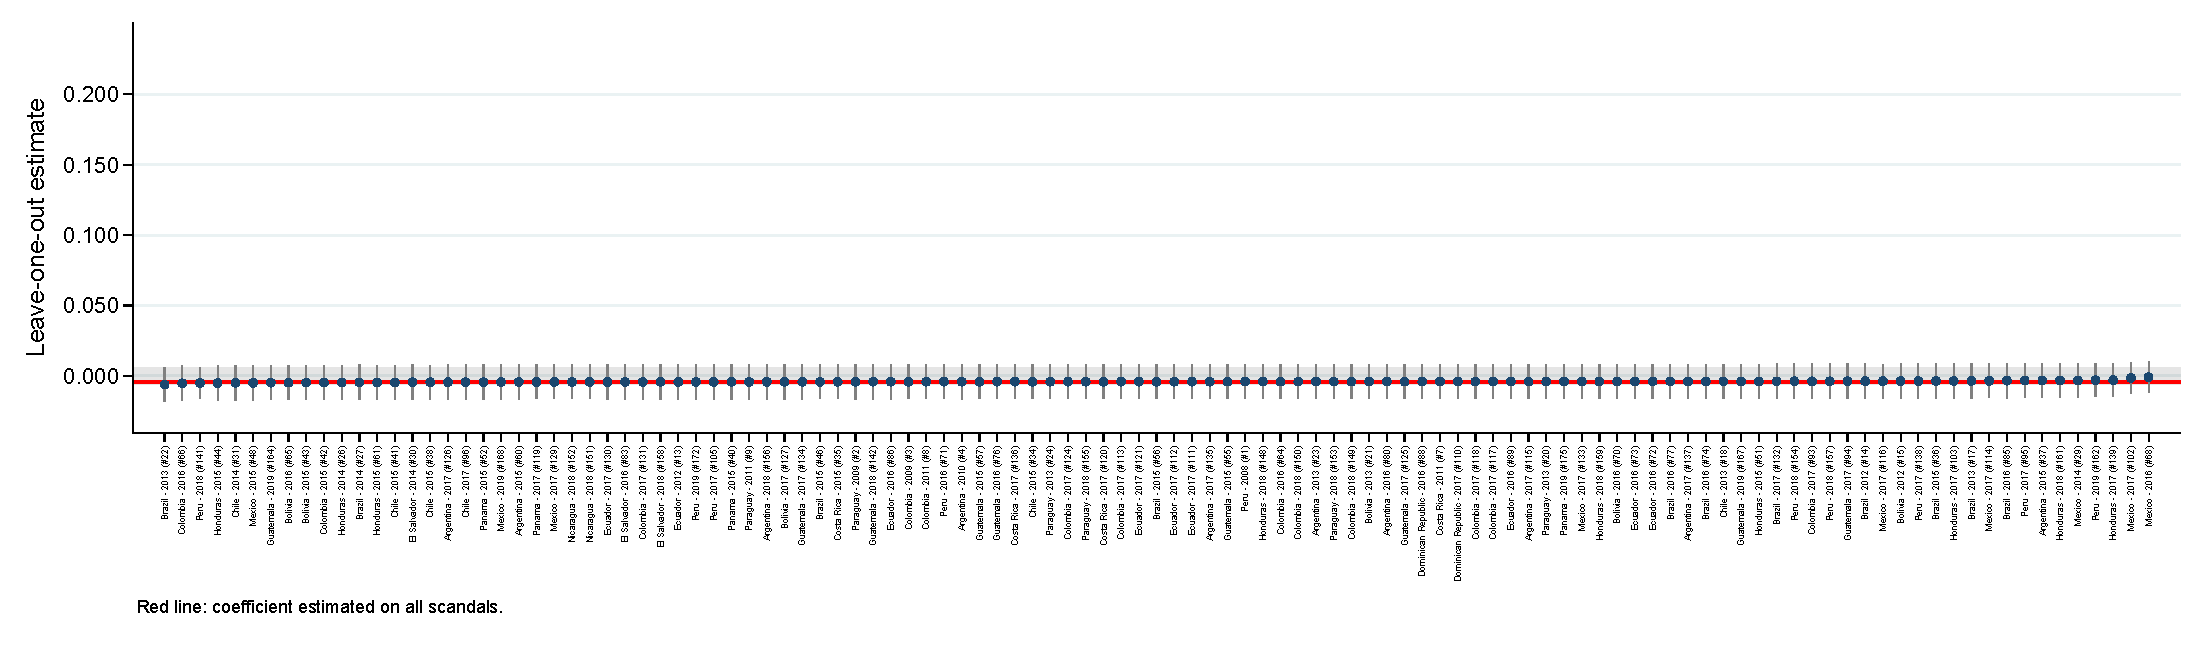
\includegraphics[width=\textwidth]{loo_scandal_beta_ona_violent_w30.pdf}
    \end{subfigure}
    \end{center}
    \footnotesize{Leave-one-out estimates of the three category coefficients of the hierarchy regression (Table~\ref{tab:sup_hierarchy}): Post $\times$ President, Post $\times$ Other Apex, and Post $\times$ Other Non-Apex, on violent protests, $\pm 30$-day window, each re-estimated dropping the labelled scandal in that category. Vertical bars are 90\% confidence intervals; the red line is the coefficient on all scandals and the faint line marks zero; the three panels share a common vertical scale. Standard errors clustered at country $\times$ year $\times$ day-bin. Sample period 2008--2019; Venezuela excluded.}
\end{figure}

\begin{figure}[htb!]
    \caption{Leave-one-out by 2008 democracy tercile.}
    \label{fig:sup_loo_demo}
    \begin{center}
    \begin{subfigure}{\textwidth}
        \caption{High democracy, dropping each high-democracy-country scandal.}
        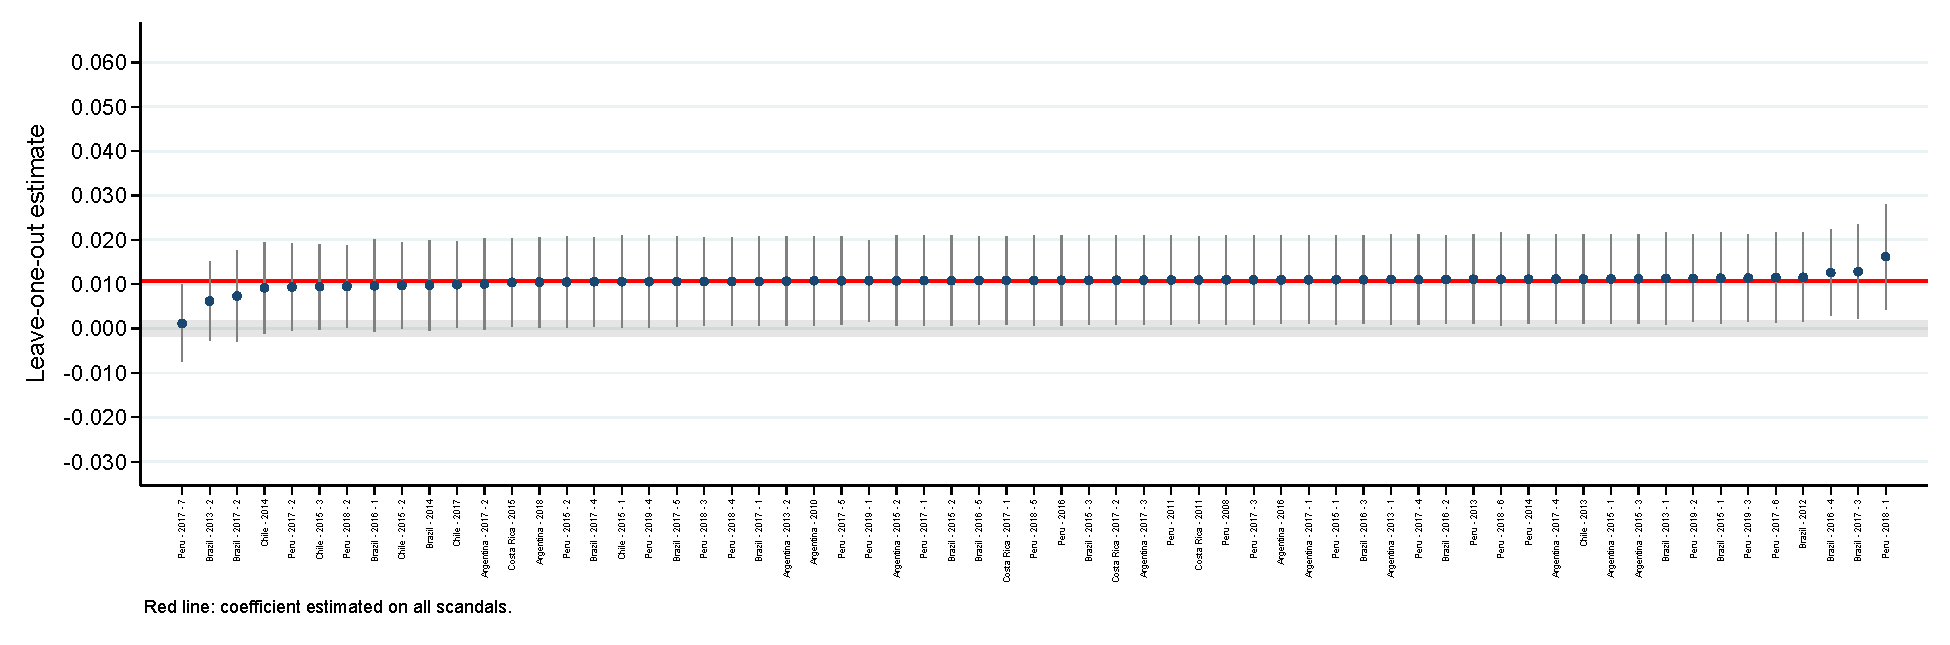
\includegraphics[width=\textwidth]{loo_scandal_beta_high_violent_w30.pdf}
    \end{subfigure} \\[4pt]
    \begin{subfigure}{\textwidth}
        \caption{Medium democracy.}
        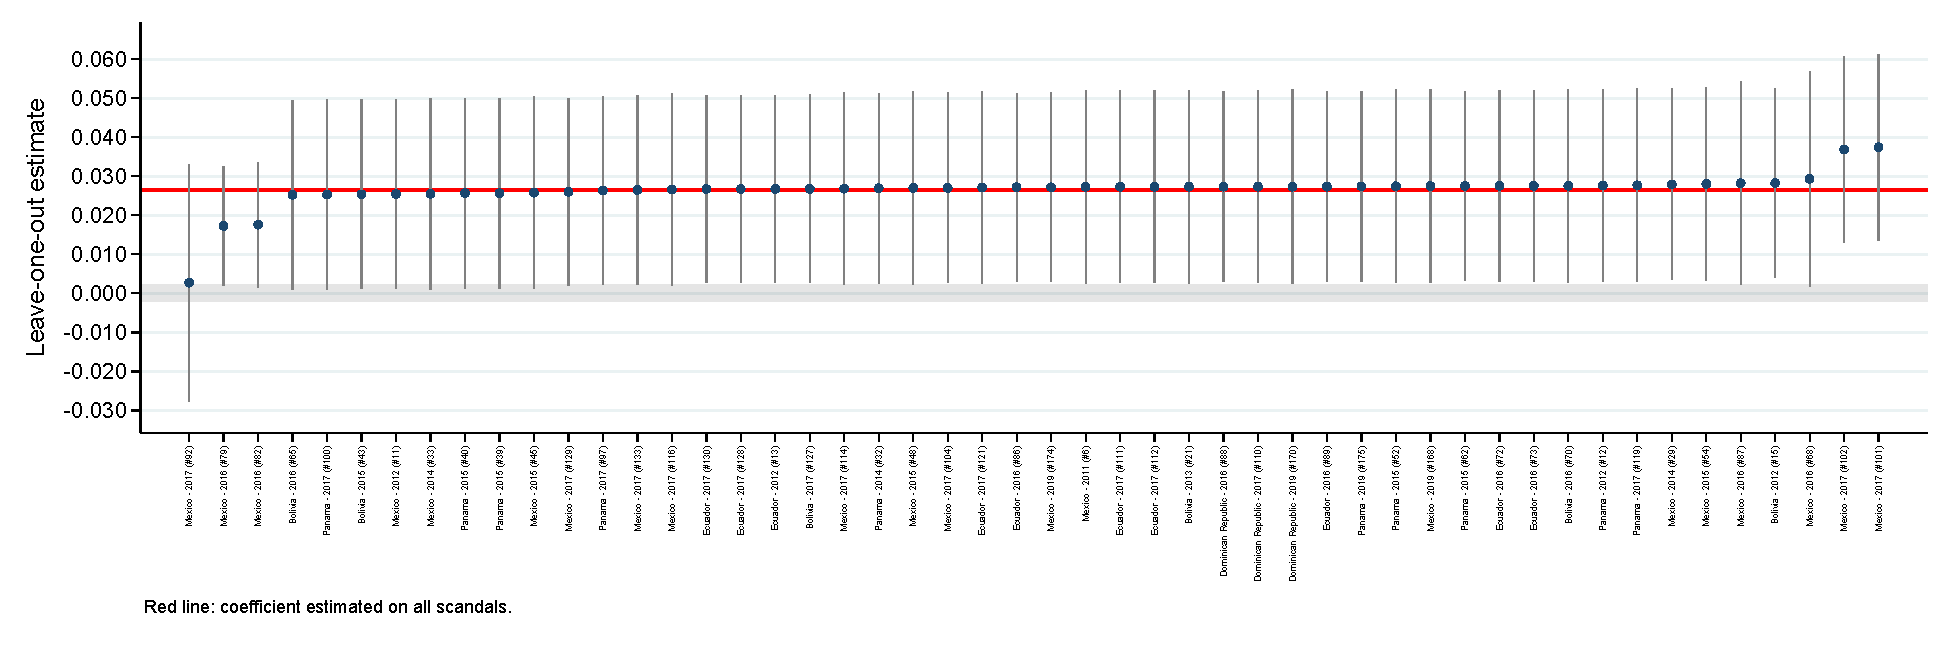
\includegraphics[width=\textwidth]{loo_scandal_beta_med_violent_w30.pdf}
    \end{subfigure} \\[4pt]
    \begin{subfigure}{\textwidth}
        \caption{Low democracy.}
        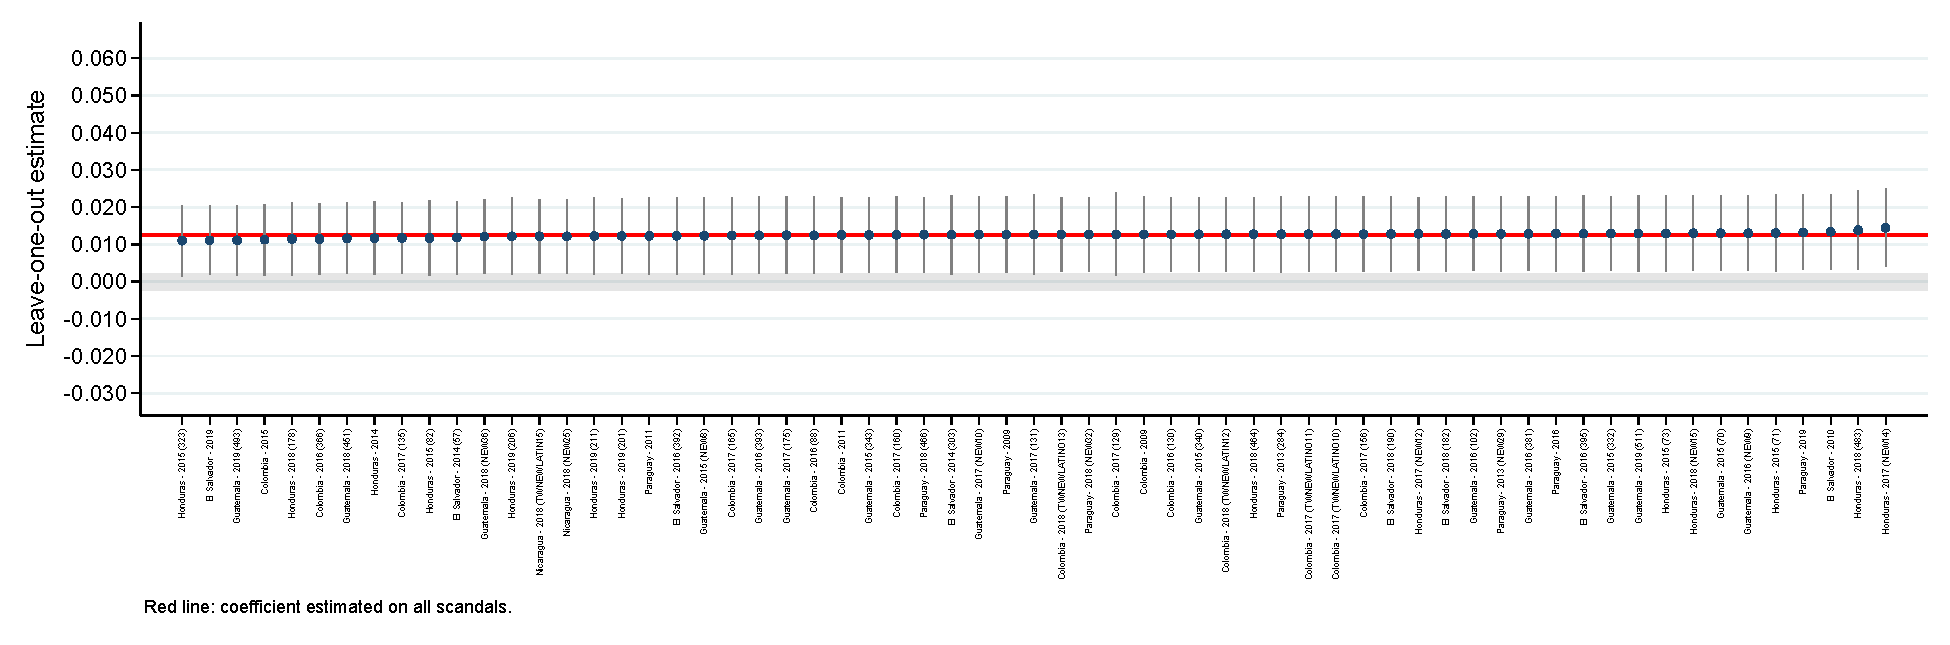
\includegraphics[width=\textwidth]{loo_scandal_beta_low_violent_w30.pdf}
    \end{subfigure}
    \end{center}
    \footnotesize{Leave-one-out estimates of the three democracy-tercile coefficients (Post $\times$ High, Medium, and Low 2008-democracy tercile, terciles of V-Dem's 2008 Electoral Democracy Index) on violent protests, $\pm 30$-day window, each re-estimated dropping the labelled scandal from that tercile. Vertical bars are 90\% confidence intervals; the red line is the coefficient on all scandals and the faint line marks zero. The three panels share a common vertical scale (on which the middle tercile shows the largest effect). Standard errors clustered at country $\times$ year $\times$ day-bin. Sample period 2008--2019; Venezuela excluded.}
\end{figure}

% ---------------------------------------------------------------------
\clearpage
\section{Placebo test: an enumerated pre-scandal cutoff}\label{sup:placebo}

If the effect really begins at the public-disclosure date and there is no anticipation, then artificially placing the post-scandal cutoff at a \emph{pre}-scandal day within the same event window should yield null coefficients. For every offset $k \in \{-T+1,\dots,-1\}$ we redefine $\widetilde{\mathrm{Post}}_{st} = \mathbf{1}\{w_{st} \geq k\}$ and re-estimate the OLS specification on the original event-window sample---no country-day is added or removed, only the treatment cutoff is shifted into the pre-scandal window. \autoref{fig:sup_placebo} plots the resulting placebo coefficients $\hat\beta(k)$ against $k$ for the full sample; Figures~\ref{fig:sup_placebo_pa} and \ref{fig:sup_placebo_na} repeat the exercise on the two subsamples of Table~\ref{tab:main}. The observed $\hat\beta$ (red horizontal line) sits above the pre-scandal placebo series for violent protests---most clearly for the Apex subsample---and near zero for peaceful protests.

\begin{figure}[htb!]
    \caption{Placebo test, full sample: violent protests, $\hat\beta(k)$ under an enumerated pre-scandal cutoff.}
    \label{fig:sup_placebo}
    \begin{subfigure}{0.48\textwidth}
        \caption{$\pm 30$-day window.}
        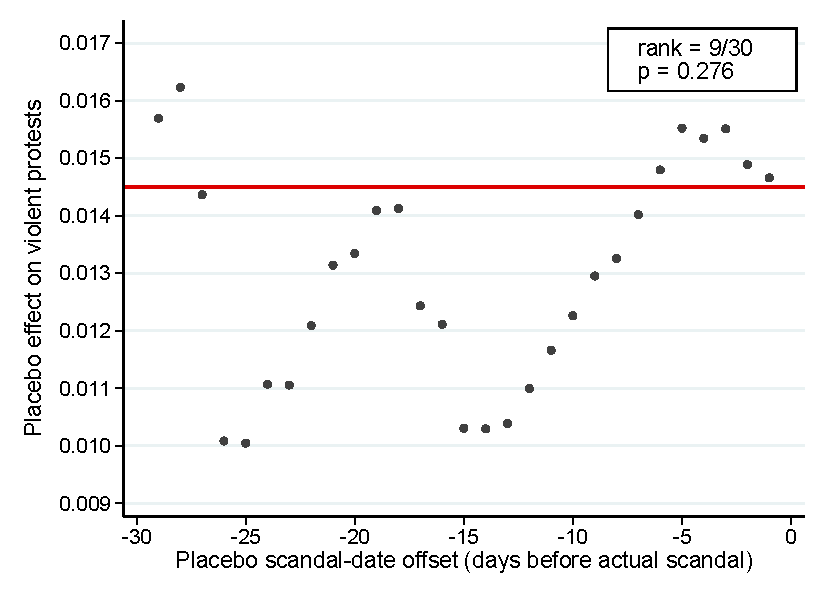
\includegraphics[width=\textwidth]{sup_placebo_within_window_hist_num_violent_MM_w30.pdf}
    \end{subfigure}\hfill
    \begin{subfigure}{0.48\textwidth}
        \caption{$\pm 60$-day window.}
        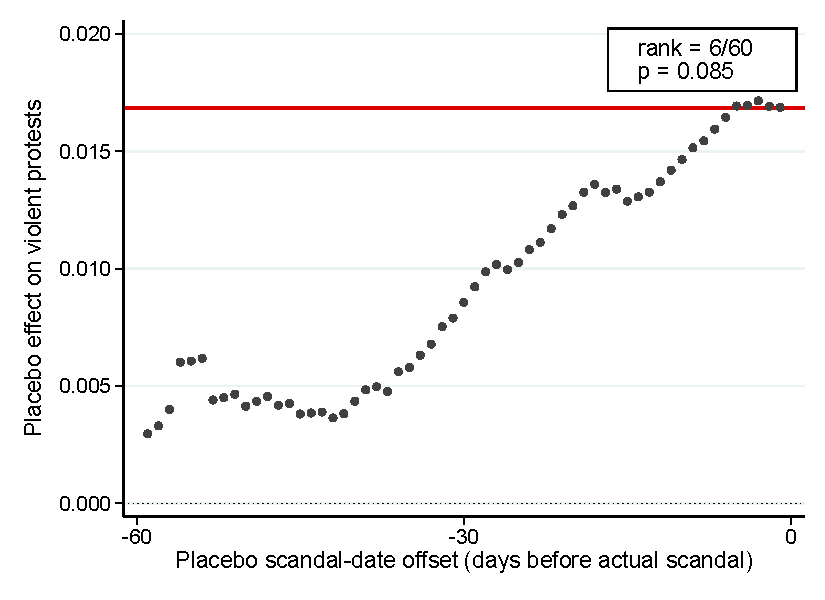
\includegraphics[width=\textwidth]{sup_placebo_within_window_hist_num_violent_MM_w60.pdf}
    \end{subfigure} \\
    \begin{subfigure}{0.48\textwidth}
        \caption{$\pm 90$-day window.}
        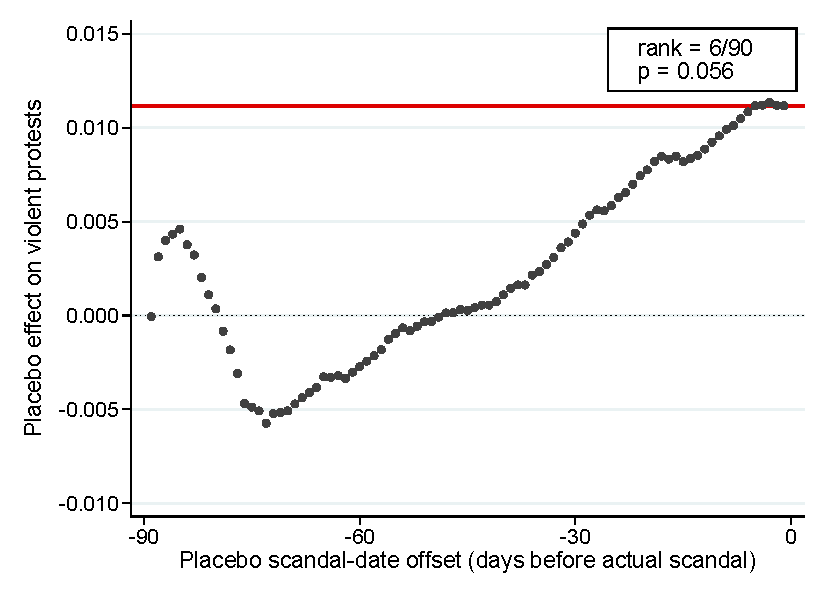
\includegraphics[width=\textwidth]{sup_placebo_within_window_hist_num_violent_MM_w90.pdf}
    \end{subfigure}\hfill
    \begin{subfigure}{0.48\textwidth}
        \caption{$\pm 120$-day window.}
        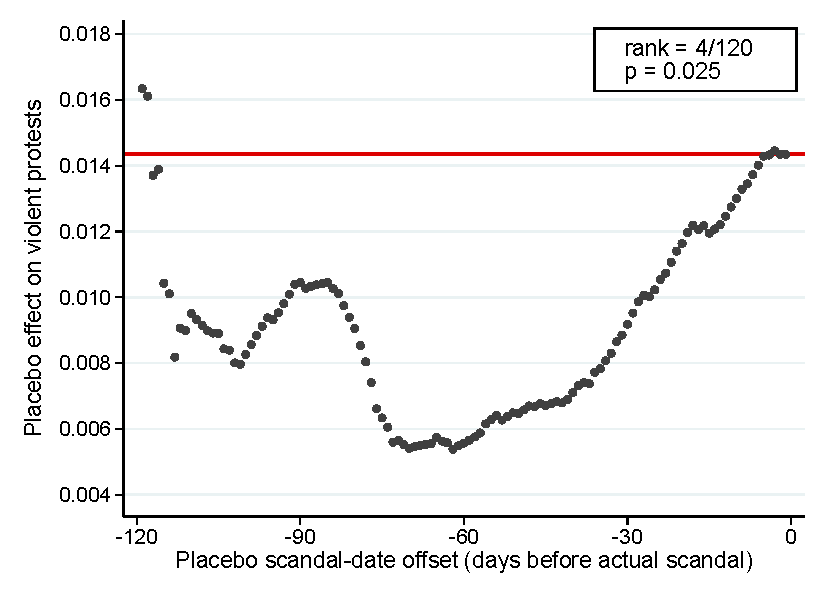
\includegraphics[width=\textwidth]{sup_placebo_within_window_hist_num_violent_MM_w120.pdf}
    \end{subfigure}
    \footnotesize{Enumerated pre-scandal cutoff placebo test for violent protests on the full sample of 176 scandals. For each offset $k\in\{-T+1,\dots,-1\}$ we replace the true post-scandal indicator with $\widetilde{\mathrm{Post}}_{st}=\mathbf{1}\{w_{st}\geq k\}$---sliding the treatment cutoff to a pre-scandal day---and re-estimate \autoref{eq:main} on the $\pm T$ event window, adding or removing no country-day. Gray circles are the resulting placebo coefficients $\hat\beta(k)$ plotted against $k$; the solid red line is the observed $\hat\beta$, the full-sample violent estimate at the $\pm T$ window; the legend gives the rank of the observed estimate among the placebos and the two-sided $p$-value. The four panels correspond to $T\in\{30,60,90,120\}$ days. Standard errors clustered at country $\times$ year $\times$ day-bin. Sample period 2008--2019; Venezuela excluded.}
\end{figure}

\begin{figure}[htb!]
    \caption{Placebo test, full sample: peaceful protests.}
    \label{fig:sup_placebo_peaceful}
    \begin{subfigure}{0.48\textwidth}
        \caption{$\pm 30$-day window.}
        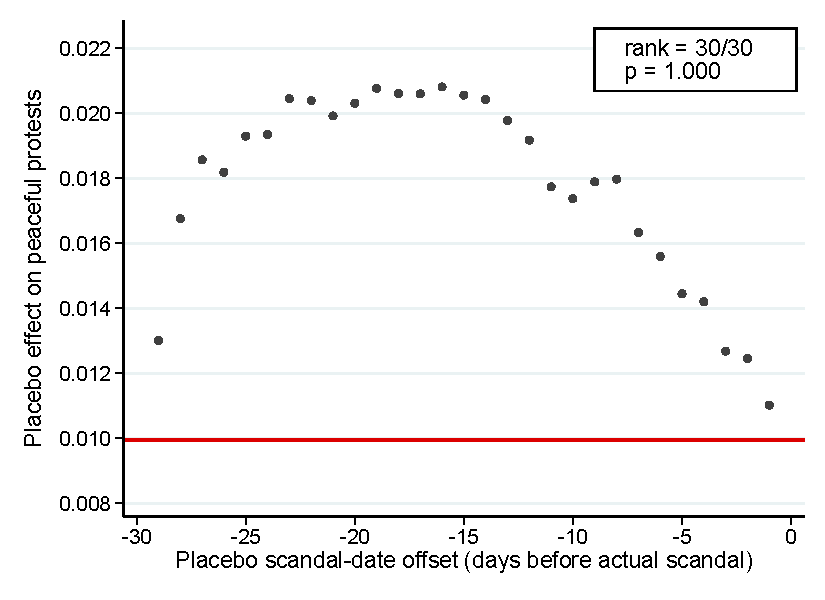
\includegraphics[width=\textwidth]{sup_placebo_within_window_hist_num_peaceful_MM_w30.pdf}
    \end{subfigure}\hfill
    \begin{subfigure}{0.48\textwidth}
        \caption{$\pm 60$-day window.}
        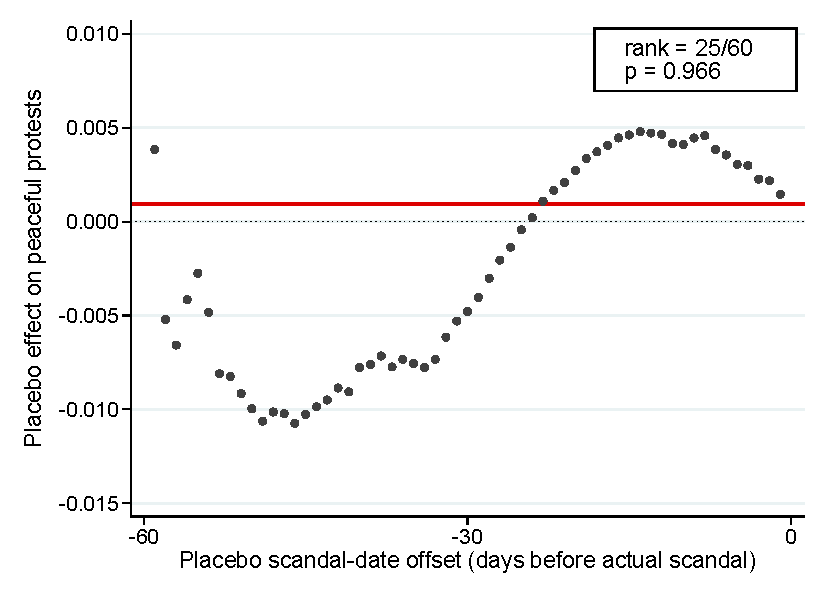
\includegraphics[width=\textwidth]{sup_placebo_within_window_hist_num_peaceful_MM_w60.pdf}
    \end{subfigure} \\
    \begin{subfigure}{0.48\textwidth}
        \caption{$\pm 90$-day window.}
        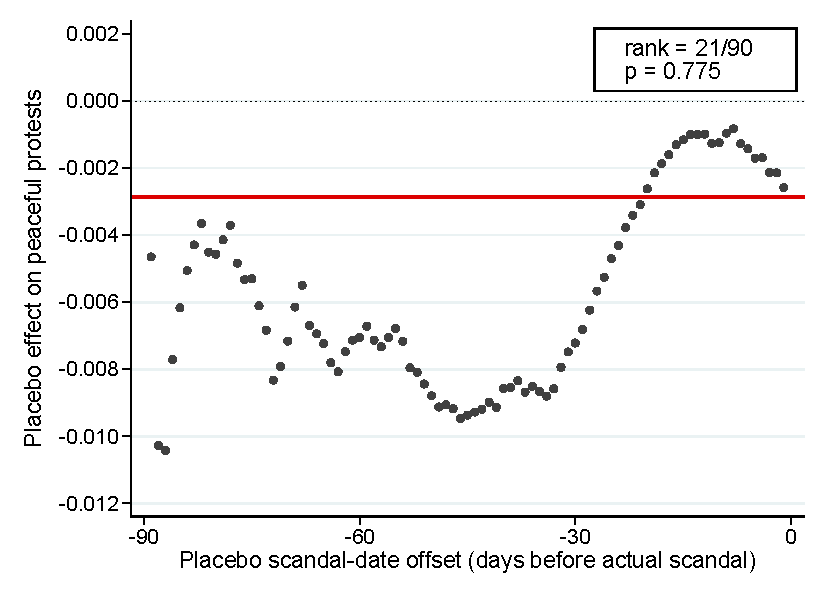
\includegraphics[width=\textwidth]{sup_placebo_within_window_hist_num_peaceful_MM_w90.pdf}
    \end{subfigure}\hfill
    \begin{subfigure}{0.48\textwidth}
        \caption{$\pm 120$-day window.}
        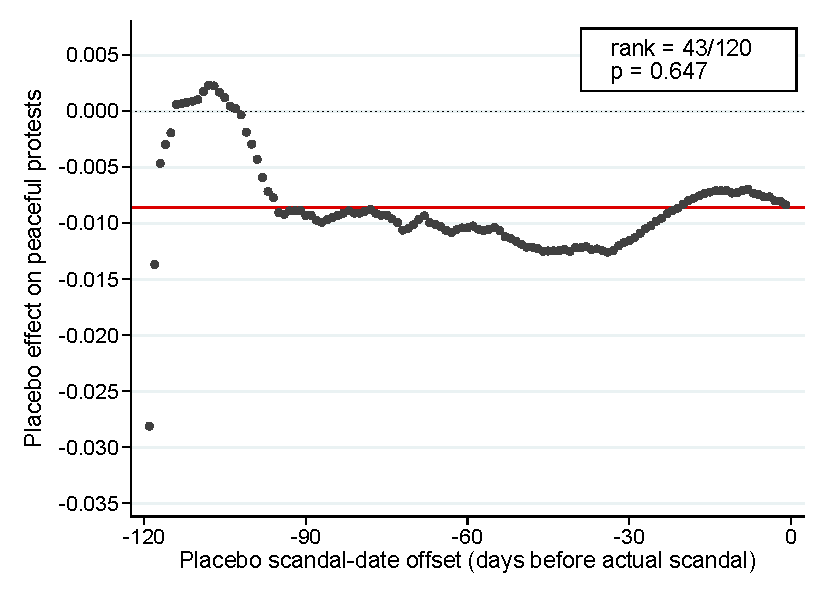
\includegraphics[width=\textwidth]{sup_placebo_within_window_hist_num_peaceful_MM_w120.pdf}
    \end{subfigure}
    \footnotesize{Enumerated pre-scandal cutoff placebo test for peaceful protests on the full sample of 176 scandals. For each offset $k\in\{-T+1,\dots,-1\}$ we replace the true post-scandal indicator with $\widetilde{\mathrm{Post}}_{st}=\mathbf{1}\{w_{st}\geq k\}$---sliding the treatment cutoff to a pre-scandal day---and re-estimate \autoref{eq:main} on the $\pm T$ event window. Gray circles are the resulting placebo coefficients $\hat\beta(k)$ plotted against $k$; the solid red line is the observed $\hat\beta$, the full-sample peaceful estimate at the $\pm T$ window; the legend gives the rank of the observed estimate among the placebos and the two-sided $p$-value. The four panels correspond to $T\in\{30,60,90,120\}$ days. Standard errors clustered at country $\times$ year $\times$ day-bin. Sample period 2008--2019; Venezuela excluded.}
\end{figure}

\begin{figure}[htb!]
    \caption{Placebo test, Apex subsample: violent protests.}
    \label{fig:sup_placebo_pa}
    \begin{subfigure}{0.48\textwidth}
        \caption{$\pm 30$-day window.}
        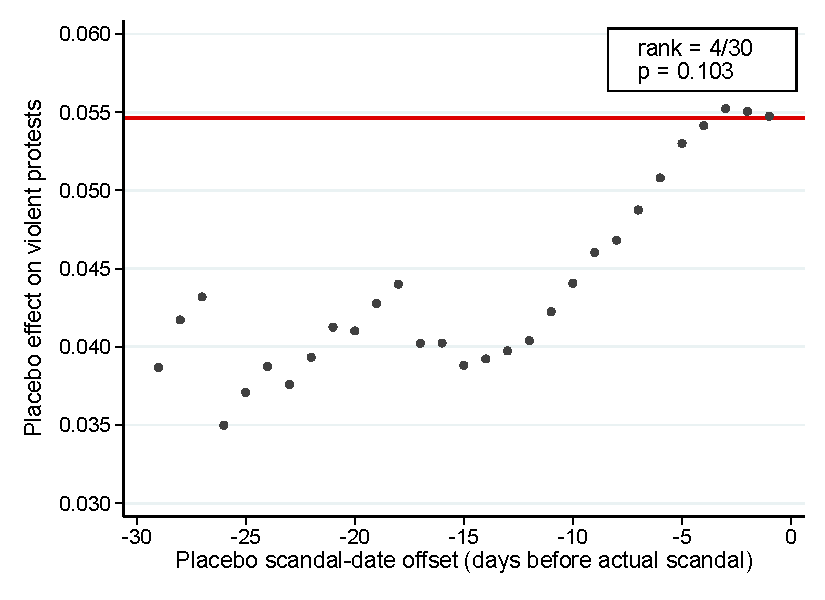
\includegraphics[width=\textwidth]{sup_placebo_within_window_hist_num_violent_MM_w30_pa.pdf}
    \end{subfigure}\hfill
    \begin{subfigure}{0.48\textwidth}
        \caption{$\pm 60$-day window.}
        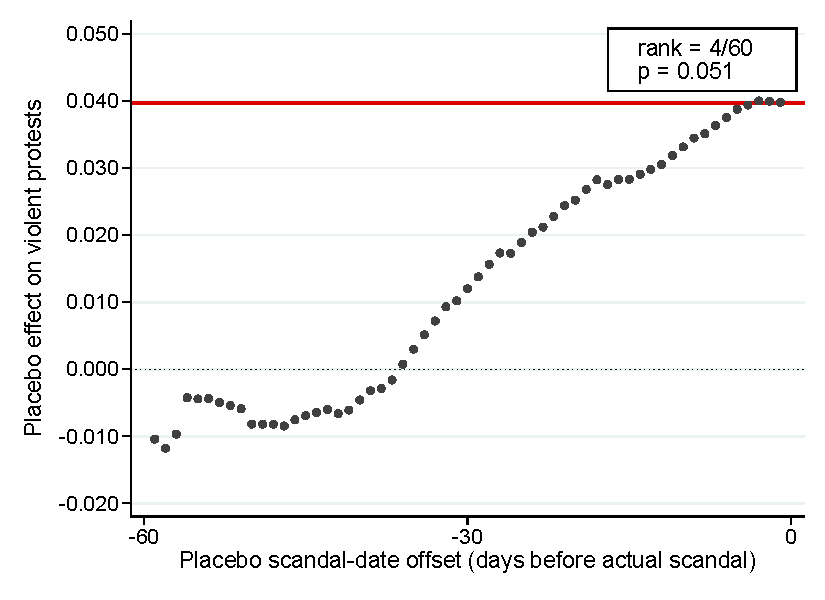
\includegraphics[width=\textwidth]{sup_placebo_within_window_hist_num_violent_MM_w60_pa.pdf}
    \end{subfigure} \\
    \begin{subfigure}{0.48\textwidth}
        \caption{$\pm 90$-day window.}
        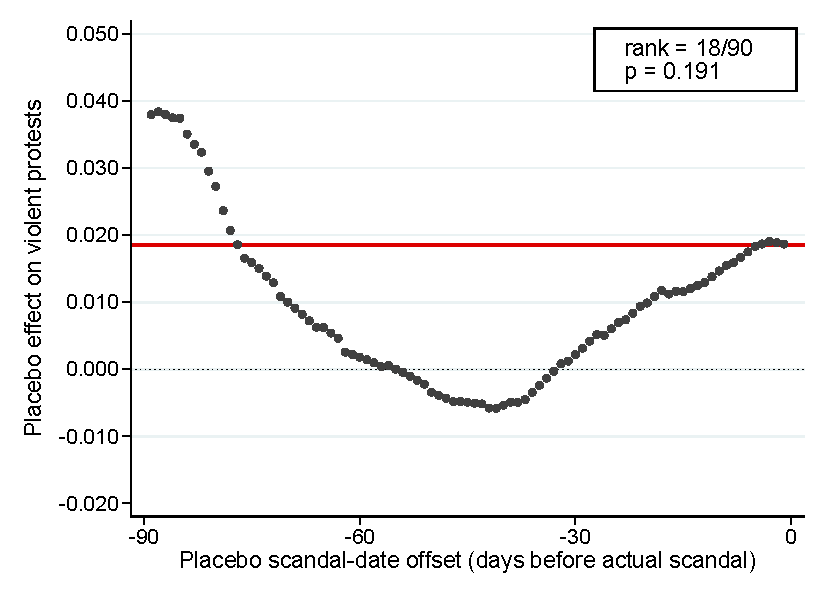
\includegraphics[width=\textwidth]{sup_placebo_within_window_hist_num_violent_MM_w90_pa.pdf}
    \end{subfigure}\hfill
    \begin{subfigure}{0.48\textwidth}
        \caption{$\pm 120$-day window.}
        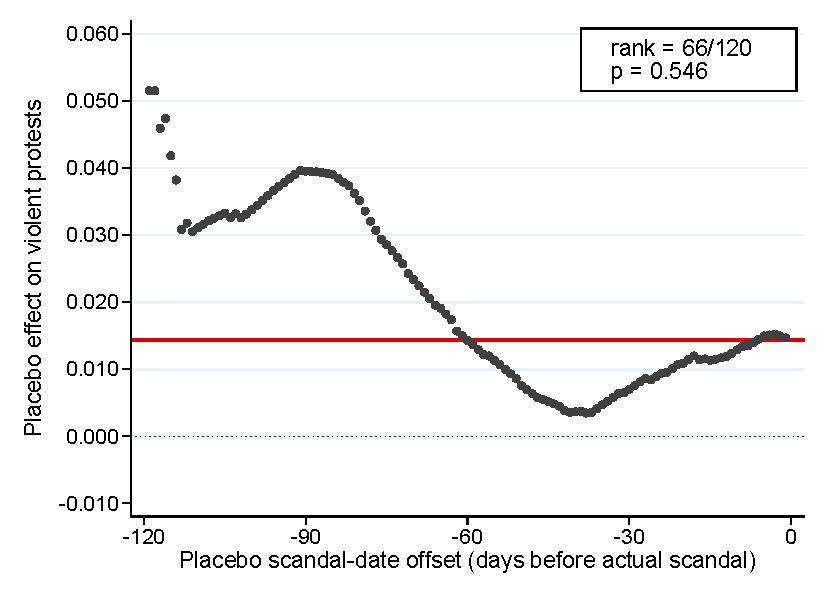
\includegraphics[width=\textwidth]{sup_placebo_within_window_hist_num_violent_MM_w120_pa.pdf}
    \end{subfigure}
    \footnotesize{Enumerated pre-scandal cutoff placebo test for violent protests on the Apex subsample (63 scandals). For each offset $k\in\{-T+1,\dots,-1\}$ we replace the true post-scandal indicator with $\widetilde{\mathrm{Post}}_{st}=\mathbf{1}\{w_{st}\geq k\}$---sliding the treatment cutoff to a pre-scandal day---and re-estimate \autoref{eq:main} on the $\pm T$ event window. Gray circles are the resulting placebo coefficients $\hat\beta(k)$ plotted against $k$; the solid red line is the observed $\hat\beta$, the apex-subsample violent estimate at the $\pm T$ window; the legend gives the rank of the observed estimate among the placebos and the two-sided $p$-value. The four panels correspond to $T\in\{30,60,90,120\}$ days. Standard errors clustered at country $\times$ year $\times$ day-bin. Sample period 2008--2019; Venezuela excluded.}
\end{figure}

\begin{figure}[htb!]
    \caption{Placebo test, Apex subsample: peaceful protests.}
    \label{fig:sup_placebo_pa_peaceful}
    \begin{subfigure}{0.48\textwidth}
        \caption{$\pm 30$-day window.}
        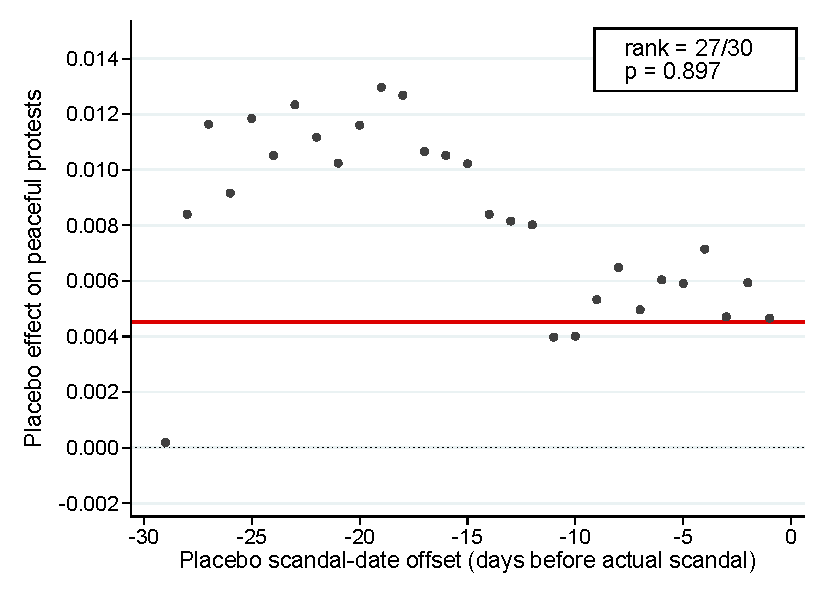
\includegraphics[width=\textwidth]{sup_placebo_within_window_hist_num_peaceful_MM_w30_pa.pdf}
    \end{subfigure}\hfill
    \begin{subfigure}{0.48\textwidth}
        \caption{$\pm 60$-day window.}
        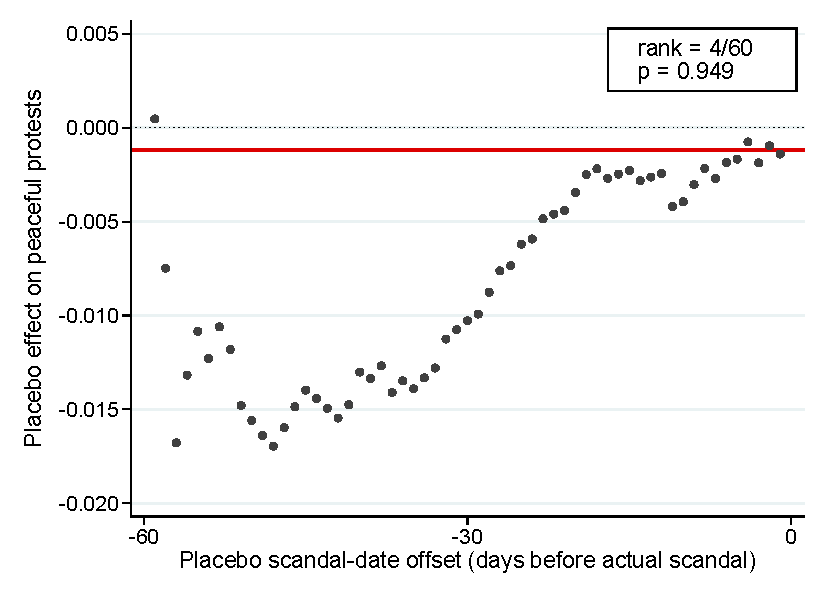
\includegraphics[width=\textwidth]{sup_placebo_within_window_hist_num_peaceful_MM_w60_pa.pdf}
    \end{subfigure} \\
    \begin{subfigure}{0.48\textwidth}
        \caption{$\pm 90$-day window.}
        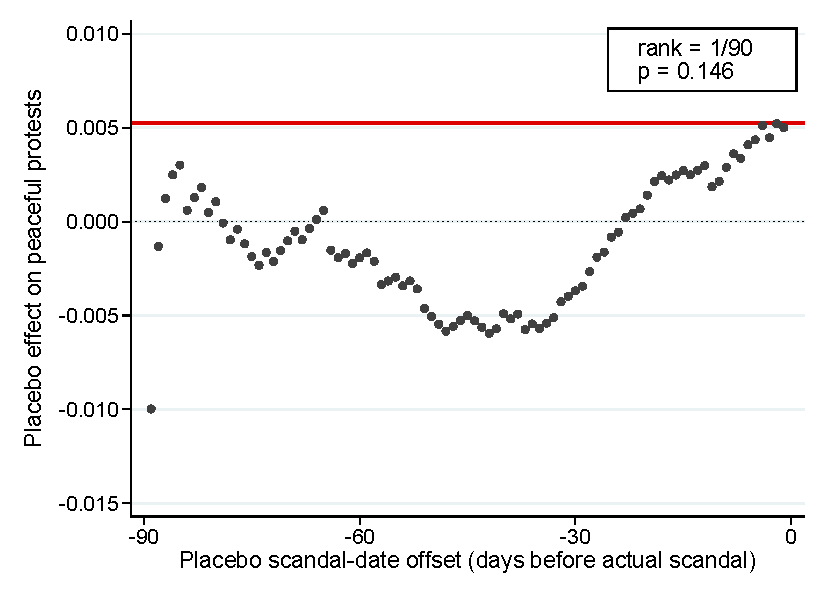
\includegraphics[width=\textwidth]{sup_placebo_within_window_hist_num_peaceful_MM_w90_pa.pdf}
    \end{subfigure}\hfill
    \begin{subfigure}{0.48\textwidth}
        \caption{$\pm 120$-day window.}
        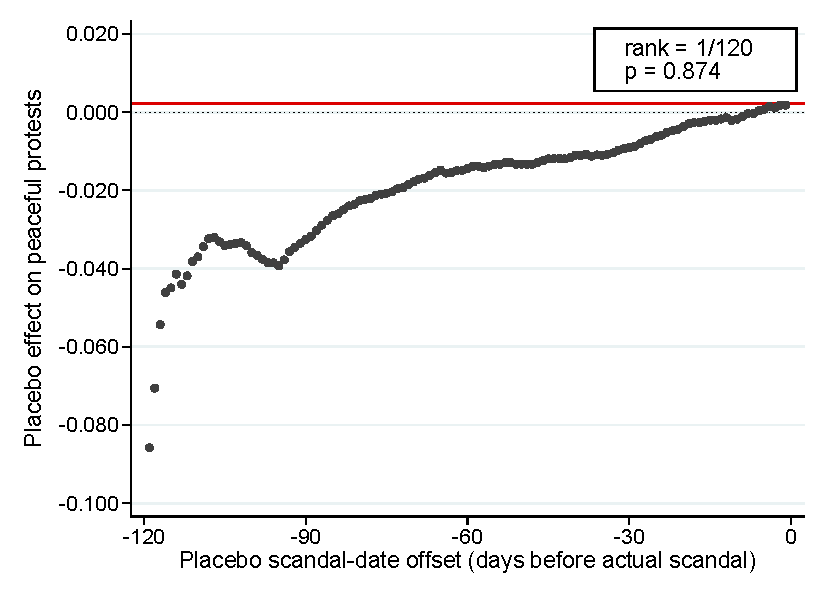
\includegraphics[width=\textwidth]{sup_placebo_within_window_hist_num_peaceful_MM_w120_pa.pdf}
    \end{subfigure}
    \footnotesize{Enumerated pre-scandal cutoff placebo test for peaceful protests on the Apex subsample (63 scandals). For each offset $k\in\{-T+1,\dots,-1\}$ we replace the true post-scandal indicator with $\widetilde{\mathrm{Post}}_{st}=\mathbf{1}\{w_{st}\geq k\}$---sliding the treatment cutoff to a pre-scandal day---and re-estimate \autoref{eq:main} on the $\pm T$ event window. Gray circles are the resulting placebo coefficients $\hat\beta(k)$ plotted against $k$; the solid red line is the observed $\hat\beta$, the apex-subsample peaceful estimate at the $\pm T$ window; the legend gives the rank of the observed estimate among the placebos and the two-sided $p$-value. The four panels correspond to $T\in\{30,60,90,120\}$ days. Standard errors clustered at country $\times$ year $\times$ day-bin. Sample period 2008--2019; Venezuela excluded.}
\end{figure}

\begin{figure}[htb!]
    \caption{Placebo test, Non-Apex subsample: violent protests.}
    \label{fig:sup_placebo_na}
    \begin{subfigure}{0.48\textwidth}
        \caption{$\pm 30$-day window.}
        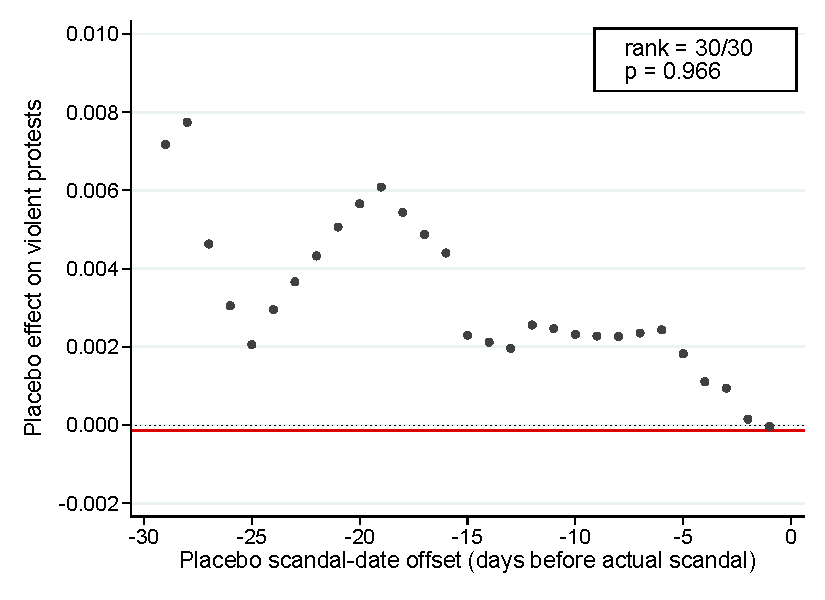
\includegraphics[width=\textwidth]{sup_placebo_within_window_hist_num_violent_MM_w30_na.pdf}
    \end{subfigure}\hfill
    \begin{subfigure}{0.48\textwidth}
        \caption{$\pm 60$-day window.}
        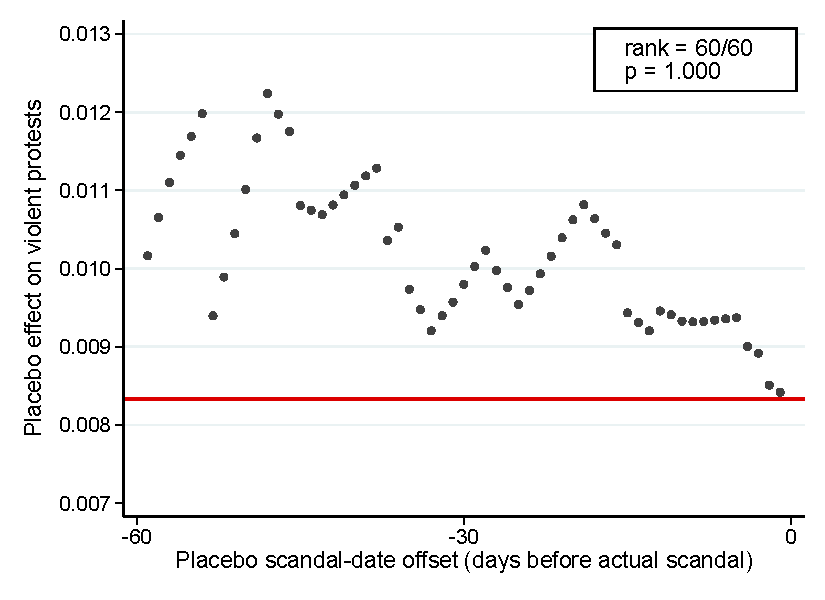
\includegraphics[width=\textwidth]{sup_placebo_within_window_hist_num_violent_MM_w60_na.pdf}
    \end{subfigure} \\
    \begin{subfigure}{0.48\textwidth}
        \caption{$\pm 90$-day window.}
        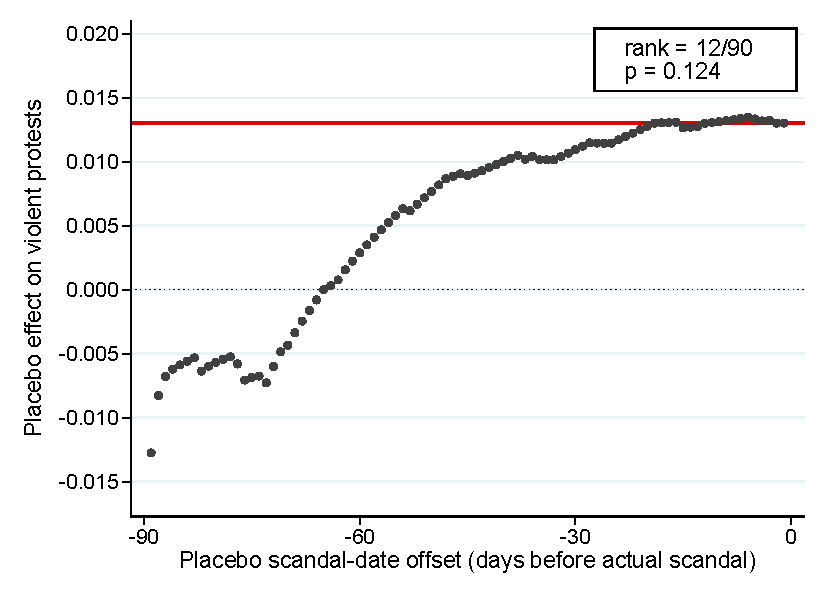
\includegraphics[width=\textwidth]{sup_placebo_within_window_hist_num_violent_MM_w90_na.pdf}
    \end{subfigure}\hfill
    \begin{subfigure}{0.48\textwidth}
        \caption{$\pm 120$-day window.}
        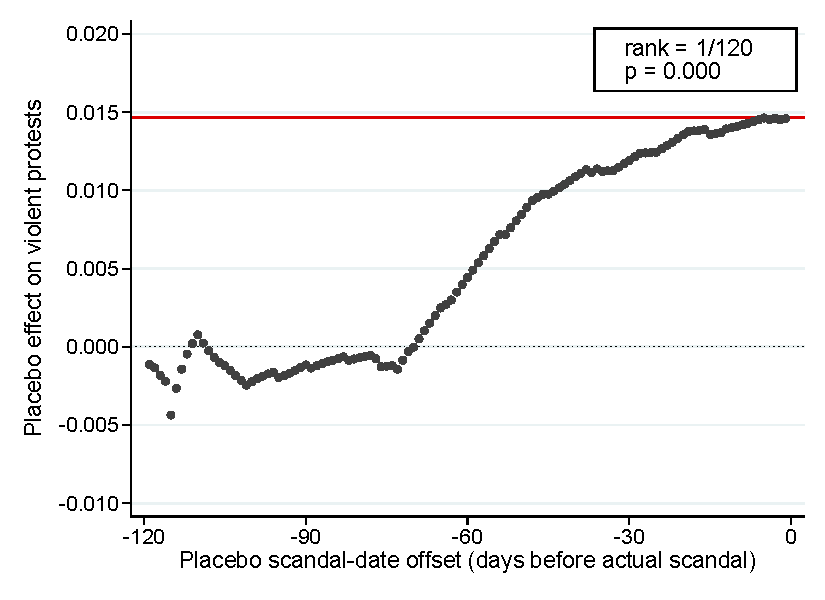
\includegraphics[width=\textwidth]{sup_placebo_within_window_hist_num_violent_MM_w120_na.pdf}
    \end{subfigure}
    \footnotesize{Enumerated pre-scandal cutoff placebo test for violent protests on the Non-Apex subsample (113 scandals). For each offset $k\in\{-T+1,\dots,-1\}$ we replace the true post-scandal indicator with $\widetilde{\mathrm{Post}}_{st}=\mathbf{1}\{w_{st}\geq k\}$---sliding the treatment cutoff to a pre-scandal day---and re-estimate \autoref{eq:main} on the $\pm T$ event window. Gray circles are the resulting placebo coefficients $\hat\beta(k)$ plotted against $k$; the solid red line is the observed $\hat\beta$, the non-apex-subsample violent estimate at the $\pm T$ window; the legend gives the rank of the observed estimate among the placebos and the two-sided $p$-value. The four panels correspond to $T\in\{30,60,90,120\}$ days. Standard errors clustered at country $\times$ year $\times$ day-bin. Sample period 2008--2019; Venezuela excluded.}
\end{figure}

\begin{figure}[htb!]
    \caption{Placebo test, Non-Apex subsample: peaceful protests.}
    \label{fig:sup_placebo_na_peaceful}
    \begin{subfigure}{0.48\textwidth}
        \caption{$\pm 30$-day window.}
        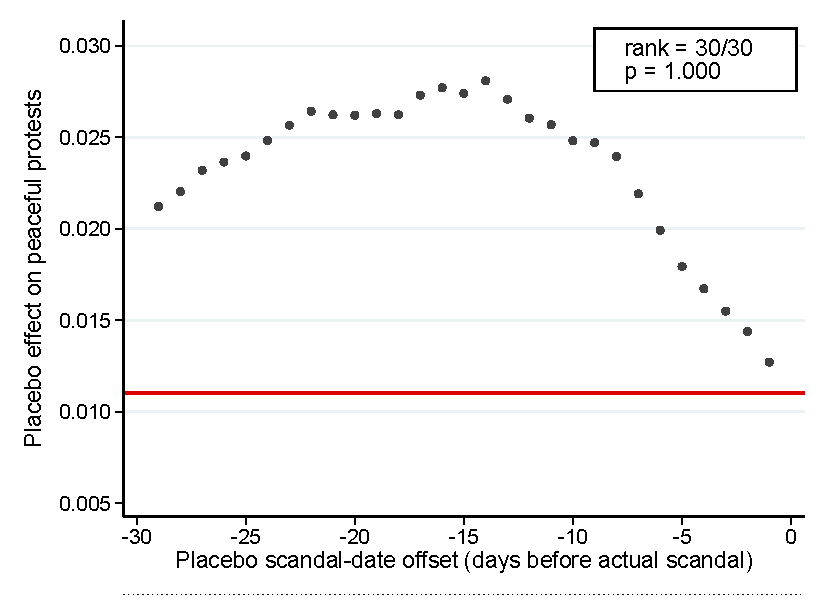
\includegraphics[width=\textwidth]{sup_placebo_within_window_hist_num_peaceful_MM_w30_na.pdf}
    \end{subfigure}\hfill
    \begin{subfigure}{0.48\textwidth}
        \caption{$\pm 60$-day window.}
        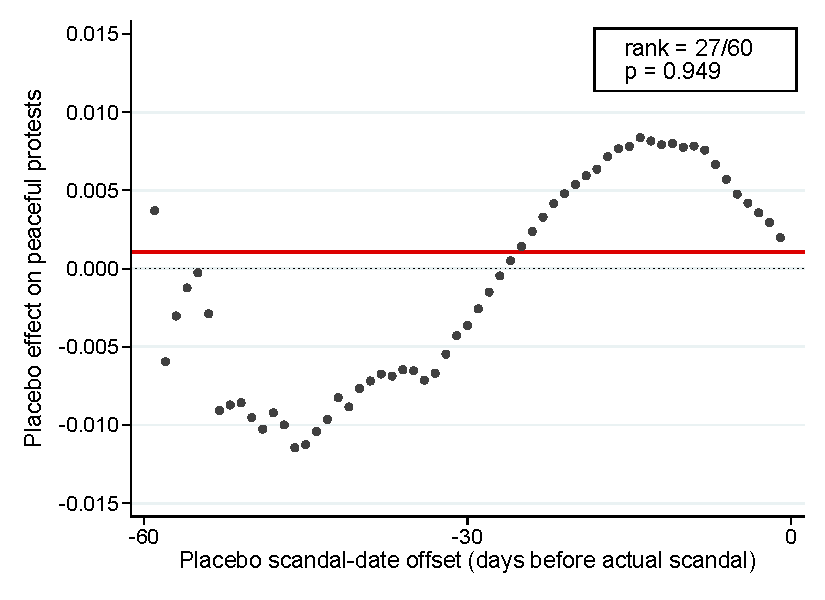
\includegraphics[width=\textwidth]{sup_placebo_within_window_hist_num_peaceful_MM_w60_na.pdf}
    \end{subfigure} \\
    \begin{subfigure}{0.48\textwidth}
        \caption{$\pm 90$-day window.}
        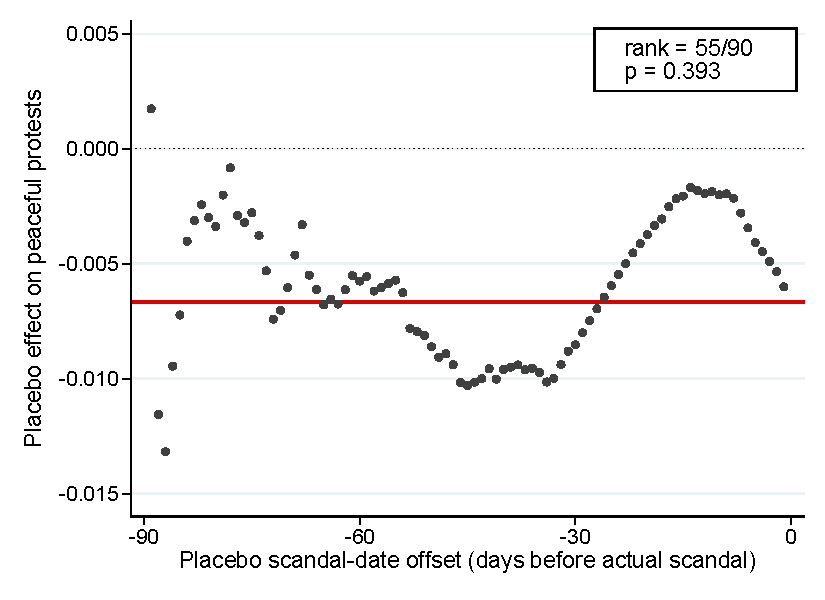
\includegraphics[width=\textwidth]{sup_placebo_within_window_hist_num_peaceful_MM_w90_na.pdf}
    \end{subfigure}\hfill
    \begin{subfigure}{0.48\textwidth}
        \caption{$\pm 120$-day window.}
        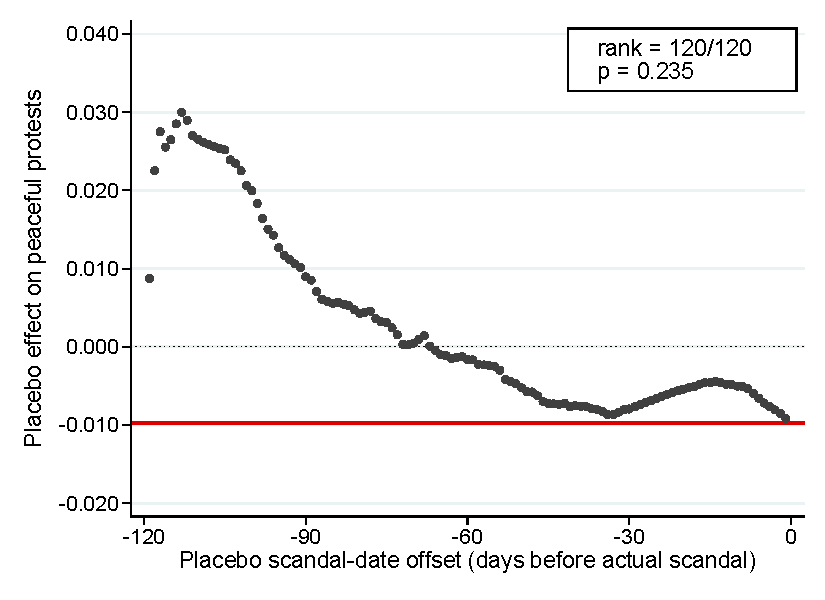
\includegraphics[width=\textwidth]{sup_placebo_within_window_hist_num_peaceful_MM_w120_na.pdf}
    \end{subfigure}
    \footnotesize{Enumerated pre-scandal cutoff placebo test for peaceful protests on the Non-Apex subsample (113 scandals). For each offset $k\in\{-T+1,\dots,-1\}$ we replace the true post-scandal indicator with $\widetilde{\mathrm{Post}}_{st}=\mathbf{1}\{w_{st}\geq k\}$---sliding the treatment cutoff to a pre-scandal day---and re-estimate \autoref{eq:main} on the $\pm T$ event window. Gray circles are the resulting placebo coefficients $\hat\beta(k)$ plotted against $k$; the solid red line is the observed $\hat\beta$, the non-apex-subsample peaceful estimate at the $\pm T$ window; the legend gives the rank of the observed estimate among the placebos and the two-sided $p$-value. The four panels correspond to $T\in\{30,60,90,120\}$ days. Standard errors clustered at country $\times$ year $\times$ day-bin. Sample period 2008--2019; Venezuela excluded.}
\end{figure}

% % ---------------------------------------------------------------------
% \clearpage
% \section{Randomization inference on the full sample}\label{sup:ri_full}

% Figure~\ref{fig:sup_ri_full} runs the permutation test of \autoref{sup:ri} on all 176 scandals pooled. Table~\ref{tab:sup_ri_percentile} then re-expresses the randomization-inference output for the full sample and the two subsamples in percentile language: for each cell it reports the percentile of the observed $\hat\beta$ within its placebo distribution (the share of placebo draws at or below the observed value), alongside the two-sided RI $p$-value. The observed violent-protest effect sits in the upper tail of its placebo distribution, most sharply in the Apex subsample.

% \begin{figure}[htb!]
%     \caption{Randomization inference, full sample.}
%     \label{fig:sup_ri_full}
%     \begin{subfigure}{0.48\textwidth}
%         \caption{Violent, $\pm 30$-day window.}
%         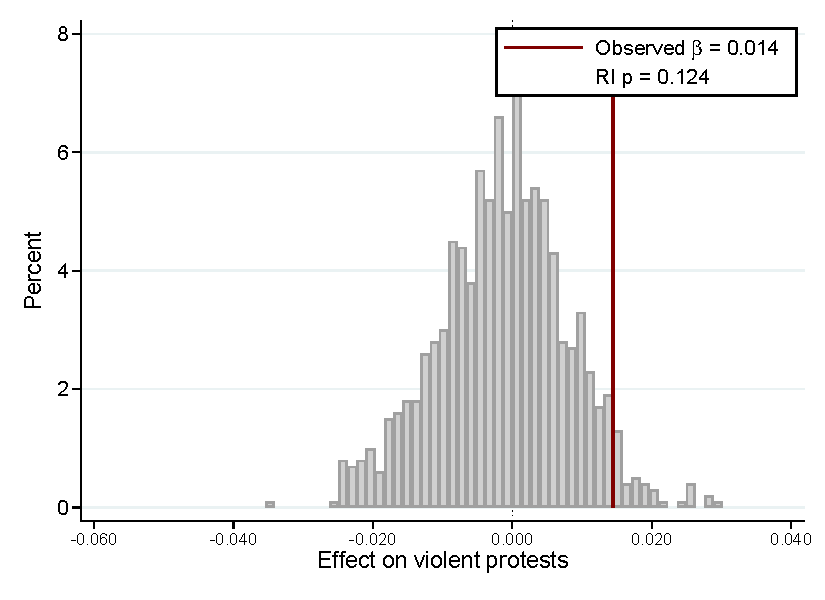
\includegraphics[width=\textwidth]{randomization_inference_hist_num_violent_MM_w30.pdf}
%     \end{subfigure}\hfill
%     \begin{subfigure}{0.48\textwidth}
%         \caption{Violent, $\pm 120$-day window.}
%         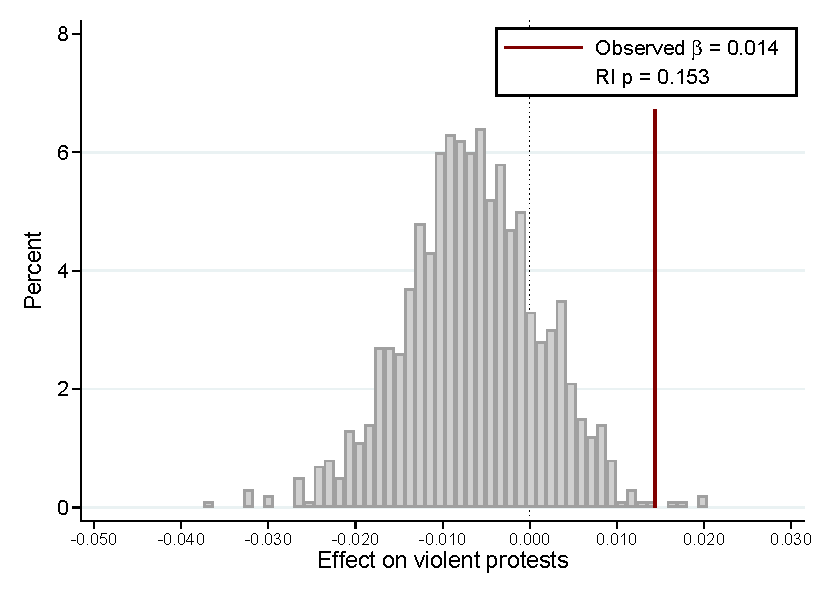
\includegraphics[width=\textwidth]{randomization_inference_hist_num_violent_MM_w120.pdf}
%     \end{subfigure} \\
%     \begin{subfigure}{0.48\textwidth}
%         \caption{Peaceful, $\pm 30$-day window.}
%         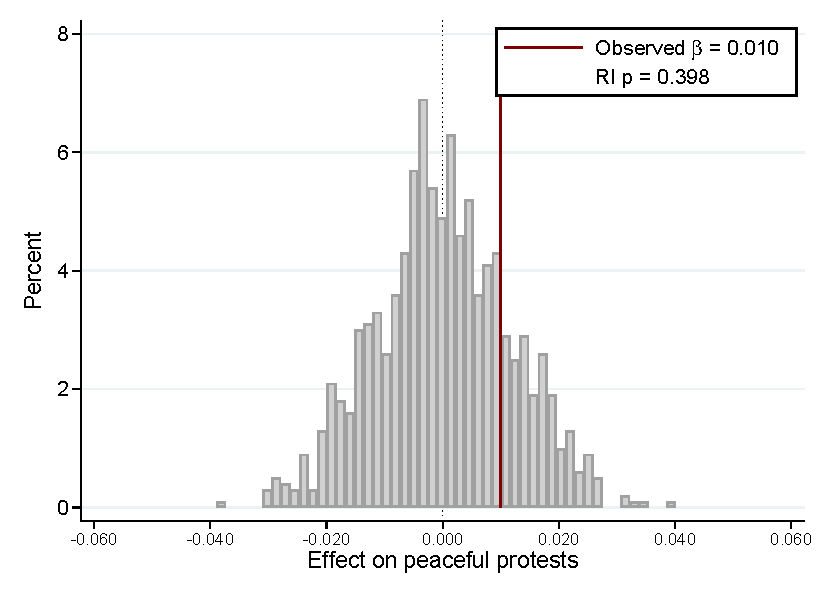
\includegraphics[width=\textwidth]{randomization_inference_hist_num_peaceful_MM_w30.pdf}
%     \end{subfigure}\hfill
%     \begin{subfigure}{0.48\textwidth}
%         \caption{Peaceful, $\pm 120$-day window.}
%         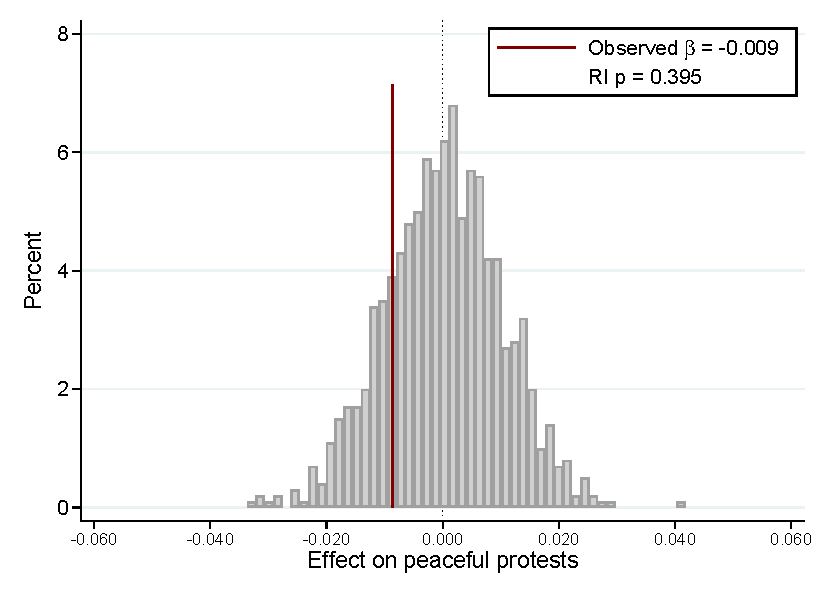
\includegraphics[width=\textwidth]{randomization_inference_hist_num_peaceful_MM_w120.pdf}
%     \end{subfigure}
%     \footnotesize{Same construction as \autoref{fig:sup_ri_pa}, on all 176 scandals. The maroon vertical line marks the observed $\hat\beta$; the legend reports the two-sided RI $p$-value. Sample period 2008--2019; Venezuela excluded.}
% \end{figure}

% \begin{table}[htb!]
%     \caption{Percentile of the observed $\hat\beta$ in the randomization-inference placebo distribution.}
%     \label{tab:sup_ri_percentile}
%     \begin{center}
%         \small{\begin{tabular}{llccc}
\toprule
Subsample & Outcome & Window & Percentile & RI $ (two-sided) \\
\midrule
Full sample & Violent & $\pm30$ & 96.3 & 0.124 \\
 & Violent & $\pm120$ & 99.6 & 0.153 \\
 & Peaceful & $\pm30$ & 80.1 & 0.398 \\
 & Peaceful & $\pm120$ & 19.4 & 0.395 \\
\midrule
President + Other Apex & Violent & $\pm30$ & 100.0 & 0.001 \\
 & Violent & $\pm120$ & 89.4 & 0.298 \\
 & Peaceful & $\pm30$ & 64.7 & 0.760 \\
 & Peaceful & $\pm120$ & 59.5 & 0.878 \\
\midrule
Other Non-Apex & Violent & $\pm30$ & 48.6 & 0.834 \\
 & Violent & $\pm120$ & 99.7 & 0.177 \\
 & Peaceful & $\pm30$ & 76.4 & 0.502 \\
 & Peaceful & $\pm120$ & 24.1 & 0.516 \\
\bottomrule
\end{tabular}
}
%     \end{center}
%     \footnotesize{For each subsample $\times$ outcome $\times$ window, ``Percentile'' is $100\times$ the share of the 1{,}000 placebo estimates at or below the observed $\hat\beta$ from Table~\ref{tab:main}; ``RI $p$'' is the two-sided randomization-inference $p$-value. Both are computed from the same placebo draws underlying Figures~\ref{fig:sup_ri_pa}--\ref{fig:sup_ri_full}. Sample period 2008--2019; Venezuela excluded.}
% \end{table}
\end{comment}

% ---------------------------------------------------------------------
\clearpage
\section{Apex scandals and democracy over time}\label{sup:dem_scandals}

As a descriptive complement to the cross-sectional democracy split, \autoref{fig:sup_dem_scandals} shows, for each of the 16 scandal countries, its V-Dem Electoral Democracy Index over 2008--2019 (solid black), with a gray vertical line at the year-month of every apex scandal in that country. For reference, each panel also draws the mean index of the bottom and top 2008-democracy terciles (short-dashed). The picture is heterogeneous: in some countries the index turns down as apex scandals cluster---Brazil falls sharply after its 2015--18 scandals and Honduras drifts lower---while in others it barely moves, most strikingly Peru, the most scandal-prone country, whose index holds near $0.8$ throughout. Notably, two of the sharpest declines (Bolivia and Nicaragua) occur in countries with \emph{no} apex scandals at all, so this is a descriptive exhibit rather than a causal estimate.

\begin{figure}[htb!]
    \caption{Electoral Democracy Index and apex-scandal timing, by country.}
    \label{fig:sup_dem_scandals}
    \begin{center}
    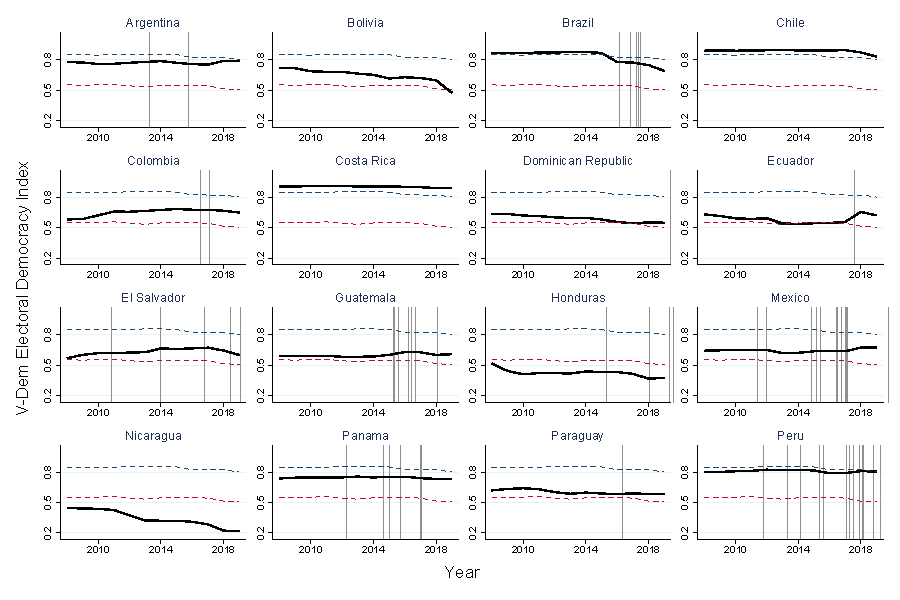
\includegraphics[width=\textwidth]{democracy_scandals_timeseries.pdf}
    \end{center}
    \footnotesize{This figure shows, in one panel per scandal country (the 16 countries in the paper's democracy tables), the evolution of democracy alongside the timing of apex scandals. The solid black line is the country's V-Dem Electoral Democracy Index (\texttt{v2x\_polyarchy}) by year, and the gray vertical lines mark the year-month of each apex-corruption scandal in that country (Bolivia, Chile, Costa Rica, and Nicaragua have no apex scandals, and hence no vertical lines). For reference, each panel also plots the mean index of the bottom (cranberry) and top (navy) tercile of the 2008 Electoral Democracy Index---the same tercile classification used in the paper's democracy tables. All panels share a common vertical scale. Sample period 2008--2019; Venezuela excluded.}
\end{figure}

% ---------------------------------------------------------------------
\clearpage
\section{Apex scandals and the Liberal Democracy Index over time}\label{sup:dem_scandals_lib}

\autoref{fig:sup_dem_scandals_lib} repeats \autoref{fig:sup_dem_scandals} using V-Dem's Liberal Democracy Index (\texttt{v2x\_libdem}) in place of the Electoral index, with the terciles re-formed from the 2008 Liberal index. The levels are lower---the liberal index is the stricter measure---but the patterns are the same: Brazil and Honduras decline as their apex scandals accumulate, Peru stays flat despite having the most scandals, and the largest falls (Bolivia, Nicaragua) again occur in countries with no apex scandals.

\begin{figure}[htb!]
    \caption{Liberal Democracy Index and apex-scandal timing, by country.}
    \label{fig:sup_dem_scandals_lib}
    \begin{center}
    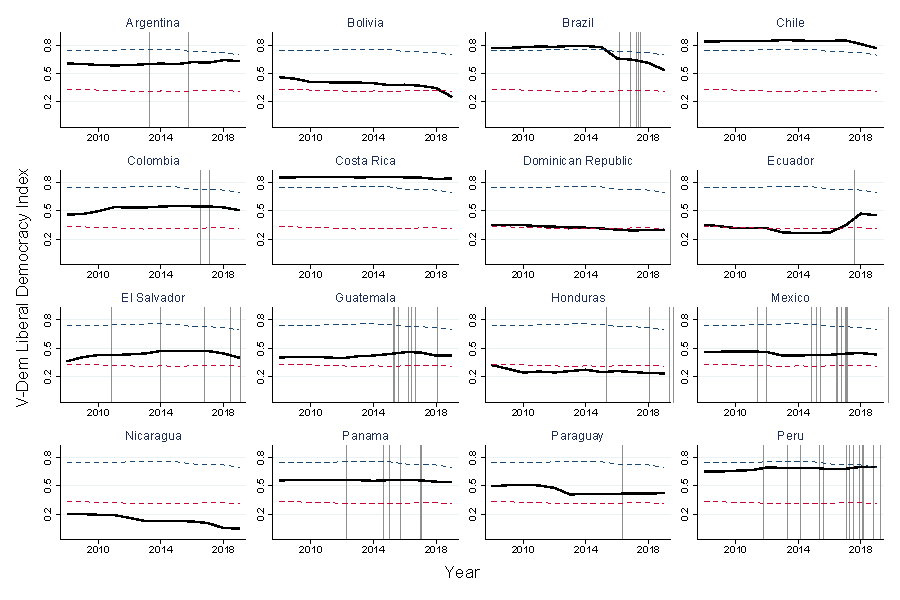
\includegraphics[width=\textwidth]{democracy_scandals_liberal.pdf}
    \end{center}
    \footnotesize{This figure reproduces \autoref{fig:sup_dem_scandals} using V-Dem's Liberal Democracy Index (\texttt{v2x\_libdem}) in place of the Electoral Democracy Index. The solid black line is the country's Liberal Democracy Index by year, and the two short-dashed reference lines are the bottom- (cranberry) and top-tercile (navy) means formed from its 2008 value; the gray vertical lines again mark the year-month of each apex-corruption scandal. All panels share a common vertical scale. Sample period 2008--2019; Venezuela excluded.}
\end{figure}

\end{document}
